\documentclass[a4j,12pt,twoside]{jreport}

%%%%%%%%%%%%%%%%%%%%%%%%%%%%%%%%%%%%%%%%%%%%%%%%%
% パッケージ宣言
%%%%%%%%%%%%%%%%%%%%%%%%%%%%%%%%%%%%%%%%%%%%%%%%%
\usepackage{graphicx}
\usepackage{times}
\usepackage{selectp}
\usepackage{epsf}
\usepackage{styles/epsbox}
\usepackage{styles/mediabb}
%\usepackage{styles/boites_exemples}
\usepackage{styles/verbatimfiles}
\usepackage{here}
\usepackage{url}
\usepackage{fancyhdr}
\usepackage{fancyvrb}
\usepackage{styles/algorithm}
\usepackage{styles/algorithmic}
\usepackage{cite}
\usepackage[dvipdfmx, usenames]{color}
\usepackage{colortbl}

\usepackage{ascmac}
\usepackage{amsmath}
\usepackage{amsthm}
\usepackage{amssymb}
\usepackage{latexsym}

\usepackage{styles/thesis}

%%%%%%%%%%%%%%%%%%%%%%%%%%%%%%%%%%%%%%%%%%%%%%%%%
% マクロ定義
%%%%%%%%%%%%%%%%%%%%%%%%%%%%%%%%%%%%%%%%%%%%%%%%%
\newcommand{\argmax}{\mathop{\rm argmax}}
\newcommand{\argmin}{\mathop{\rm argmin}}
\renewcommand{\bibname}{参考文献}

%% myマクロ
%\input{mymacros}

%% マージン設定
%\oddsidemargin=17mm
%\evensidemargin=-4mm

%%%%%%%%%%%%%%%%%%%%%%%%%%%%%%%%%%%%%%%%%%%%%%%%%
% 本文開始
%%%%%%%%%%%%%%%%%%%%%%%%%%%%%%%%%%%%%%%%%%%%%%%%%
\begin{document}
\newtheorem{defi}{Definition}[section]
\newtheorem{thy}{Theorem}[section]

\pagestyle{fancyplain}

\newlength{\oldtextwidth}
\setlength{\oldtextwidth}{\textwidth}
\setlength{\textwidth}{40zw}

% タイトル
\thispagestyle{empty}
\setcounter{page}{0}

\def \title{MissionForest: 組織内外における\\協働支援のためのタスク構造化システムの試作}
\def \author{後藤~誉昌}
\def \date{\today}
\def \teacher{白松~俊}
\def \teacherrank{准教授}
\def \belong{名古屋工業大学\\工学部 情報工学科}
\def \year{23}
\def \regnum{24115054}

\def\sizeLL#1{\Huge #1}
\def\sizeL#1{\LARGE #1}
\def\sizeM#1{\Large #1}
\def\sizeS#1{\large #1}

\def\REYrule{\hbox to 5cm{\leaders\hrule height 1pt\hfill}}
\newbox\REYbox
\def\announce#1{
  \setbox\REYbox=\hbox{\REYrule\quad{\Large\bf #1}\quad\raise3pt\REYrule}%
  \gdef\REYbigrule{\hbox to \wd\REYbox{\leaders\hrule height 1pt \hfill}}%
  \centerline{\raise3pt\REYrule\vspace*{2mm}\quad{\LARGE #1}\quad\raise3pt\REYrule}}
\def\endannounce{\par\centerline{\REYbigrule}}

\begin{titlepage}
 \begin{center}
 %\renewcommand{\baselinestretch}{1.0}
  \vspace*{5mm}
  \sizeLL{卒業論文}\\
  \vspace*{10mm}
  \begin{announce}{(題~~目)}
   \sizeL{\title}\\
  \end{announce}
  \vspace*{20mm}
  \sizeM{指導教員~~~~~}\sizeL{\teacher}\sizeM{~~\teacherrank}\\
  %\vspace*{40mm} % 題目が2行の場合
 % \vspace*{30mm} % 題目が3行の場合
 \vspace{10mm}
  \sizeM{\belong}\\
  \vspace*{10mm}
  \sizeM{平成 \year 年 4 月 入学}\\
  \vspace*{3mm}
  \begin{table}[H]
    \begin{center}
     \begin{tabular}{cl}
      \sizeM{(学籍番号)} & \sizeL{{\underline{~~ \regnum ~~}}} \\
      \sizeM{(氏~名)} & \sizeL{\underline{~~ \author ~~}} \\
     \end{tabular}
    \end{center}
   \end{table}
  \vspace*{10mm}
  \sizeS{(提出日:~\today)}
  % \sizeS{(提出日:\ ~平成28年2月8日)}
 \end{center}
\end{titlepage}

\cleardoublepage

% タイトル以降用パラメータ
\setlength{\oddsidemargin}{17mm}
\setlength{\evensidemargin}{-4mm}
\setlength{\textwidth}{\oldtextwidth}

\cleardoublepage

%ここからページ数開始
\pagenumbering{arabic}
\cleardoublepage

% アブストラクト
%!TEX root = ../../main.tex
\chapter*{論文要旨}
\label{chap0}
\addcontent{論文要旨}
大学の研究室では,教員の指示だけに頼らず主体的に考えて研究できる学生の育成が求められている.
しかし研究生活に慣れていない学生にとってはうまく研究が進まないことも多く,また教員も逐一フォローアップできていない現状がある.
そこで,「どのような課題をどのようなアプローチで解決しようとしているか」を日常的に学生自身がデータ化し共有することで,教員や他学生とのコミュニケーションを支援し,
協働を促進することができると考える.
学生の研究目標を公開・共有することによって,教員による進捗の把握や,学生の自律性向上,学生同士の協働の促進を目的としている.
また学外に対しても,研究アプローチや研究成果を公開することによって,外部組織との連携やアウトリーチ活動にも活用でき,公益活動にも研究シーズを活用できる可能性がある.

本研究ではこれまで,公益活動やシビックテックといった分野を対象とし,公共圏で目標を共有するWebシステム「ゴオルシェア」[1]を開発・運営してきた.
従来のゴオルシェアは組織横断的な協働を想定しており,目標データを全てオープンデータ化していた.
しかし,組織内での日常的な活動は公開に適さないものも多いため,日常的には使いにくいという問題点があった.
また,目標を階層化したツリー構造の入力操作が直感的でないという問題点もあった.
そこで本稿で試作する新システム「MissionForest」では,
(1)組織内部の日常的な活動を非公開な目標ツリーとして記録し,
(2)外部発表後にツリー構造の全体もしくは一部のみをLODとしてオープンデータ化可能にする.
さらに,(3)目標ツリーを直感的操作で作成・編集可能にする.

\cleardoublepage

% 目次
% 目次
\markboth{目 次}{目 次}
\tableofcontents

% 図目次
\listoffigures
\markboth{図 目 次}{図 目 次}

% 表目次
\listoftables
\markboth{表 目 次}{表 目 次}

\cleardoublepage

% 第1章 序論
%!TEX root = ../../main.tex
\chapter{序論}
\label{chap:intro}

\section{本研究の背景}
本システムでは,まずはケーススタディとして大学の研究室を対象とする.
学生の研究目標を公開・共有することによって,教員による進捗の把握や,学生の自律性向上,学生同士の協働の促進を目的としている.
また作成されたデータは後から一般公開できるので,外部組織との連携やアウトリーチ活動にも活用でき,これまでのゴオルシェアが対象とするような公益活動にも研究シーズを活用できる可能性がある.
初期段階では本研究室内で試用し,有用性を検証する.

\section{本研究の目的}
組織を超えた協働プロジェクトを円滑に進行させるには,(1)プロジェクト全体のタスクを俯瞰できる,(2)後から参加した人でも議論に参加しやすいような議事録作り,(3)誰が何をどこまでやったのかが把握できる進捗管理,という3つの要件を満たす必要がある.
このような要件を満たすシステムは”プロジェクト管理システム”と呼ばれ,有償無償問わず数多く存在する.
上記のような従来型のプロジェクト管理システムの機能に加え,プロジェクトの成果を公開することで,2次活用や外部組織との連携に役立てられることができれば,新たな協働を生む可能性がある.
そこで新システムMissionForestの試作により,新たな協働を生み,協働を支援できるようなプロジェクト管理システムを目指す.
プロジェクトの目標階層は,ゴオルシェアを踏襲してLinked Dataとして構造化した上で,ゴオルシェアよりも詳細に公開/非公開を制御できる機構を目指す.

\subsection{システム構成}
本システムのシステム構成を図\ref{img:system_architecture}に示す.
ユーザーの認証情報やミッションのすべての情報は,まずはメインDBに保存される.次に,タスクごとに設定されたアクセス権限により,LODとしてRDFストアにコピーされる.
\begin{figure}[t]
	\begin{center}
		\includegraphics[width=0.9\linewidth]{assets/img/system_architecture.png}
		\caption{システム構成図}
		\label{img:system_architecture}
	\end{center}
\end{figure}

\section{本論文の構成}
本論文の構成を以下に示す.
第2章では関連研究や関連システムと本研究の動作・開発環境について述べる.
第3章では直感的にツリーを作成できるインターフェースについて述べる.
第4章ではLODでの公開機構について述べる.
第5章では類似タスクの推薦機構について述べる.
第6章では前章までで述べたシステムの評価実験の結果をまとめる.
第7章で本研究をまとめる.

\cleardoublepage

% 第2章 動作・開発環境と関連研究
%!TEX root = ../../main.tex
\chapter{関連研究と動作・開発環境}
本章では本研究の関連研究と動作・開発環境について述べる.

\section{関連研究}
本研究と関連のある研究やシステムを紹介する.

\subsection{タスク階層構造}

\subsubsection{Work Breakdown Structure}
Work Breakdown Structure(WBS)とは,プロジェクトマネジメントで計画を立てる際に用いられる手法の一つで,プロジェクト全体を細かい作業に分割した構成図.
「作業分割構成」,「作業分解図」などとも呼ばれる.
WBSでは,まずプロジェクトの成果物をできるだけ細かい単位に分解していく.
その際,全体を大きな単位に分割してから,それぞれの部分についてより細かい単位に分割していき,階層的に構造化していく.
青果物の細分化が終わったら,それぞれの部分を構成するのに必要な作業を考え,最下層に配置していく.

\subsubsection{前提条件ツリー}
前提条件ツリー(Prerequisite Tree)\cite{zentei}の構成要素には,実現すべき目標と中間目標,そして目標を実現する上での障害がある.
前提条件ツリーで扱う関係は必要関係と克服関係である.
必要関係では,上位の目標を実現するためには下位の目標が必要であることを表す.
これに対して克服関係では上位の目標の障害を下位の中間目標によって解決できることを表す.
新たなシステムが成功するための前提条件を予め明らかにするために作成するのが前提条件ツリーである.

\subsection{プロジェクト管理システム}

\subsubsection{ゴオルシェア}
ゴオルシェア\cite{shiramatsu2016}とは,社会課題とその解決目標,さらにその部分目標をLOD化して共有するためのWebサービスである.
「誰がどんな課題に注目しているのか」「誰が何を目指して動いているのか」を一般市民が自ら入力して共有することで,
方向性の似た潜在的協力者を探すことができ,さらに有力者の目標を共有し,近未来社会像の透明性向上を図る.
LODの枠組みによって,社会課題と解決目標の関係や,その部分目標との関係,協力者との関係などを紐付けし,似た目標を探せるようにした.
多くの利害関係者が絡む社会問題を解決するためには,組織横断的な協働が不可欠であり,
従来のSNSには方向性の似た潜在的協力者を探す機能がなかったので,このようなシステムがあれば,
(1) 身の回りの社会課題や目指す目標を一般市民が公開&共有して,似た方向性の人々を探せるようにする,
(2) 断片的なニュースから,社会課題や有力者の目標を抽出&共有して,世の中の動きの透明性を向上させる,
ことができる.

\subsubsection{ナレッジコネクター}
ナレッジコネクター(Knowledge Connector)は,全国的に行われているオープンデータを活用したイベントの成果等を集約し
,一元的に検索を可能にするとともに,アイディアやアプリを創出した人材とビジネスパートナーとのマッチングを支援するためのサイト.
同じような課題を抱えている人,何かをやりたいと思っているが何から手をつけていいかわからない人,もしかしたら連携できる人やコミュニティを見つけることができる.

\subsubsection{みらいらぼ}
みらいらぼ\cite{sengoku2016}とは,共創の場を支援する集合知プロジェクト支援システムである.
みらいらぼは,Webアプリケーションであり,Web上でプロジェクトの作成,共有,およ ゙共創をすることができる.
また,みらいらぼはSNSとの連携が可能であり,多くの多様な人たちとプロジェクトの共有を行うことができ,集合知を用いてプロジェクトを進めることができる.
さらに,Web上だけでなく学会と合わせてみらいらぼを使うことによって,より共創を起こすことが可能である.

\subsection{合意形成システム}

\subsubsection{COLLAGREE}
COLLAGREE\cite{ito2016}とは,離れた場所にいる人々がweb上での議論を通して合意形成をはかるシステムである.
投稿されたつぶやきがシステムによって意見集約され,合意形成を行います.
限られた人々が一室に集まって行う従来の閉じられた議論ではなく,多くの人々がいつでもインターネット上で開かれた議論を行えることを目指している.

\section{動作・開発環境}

\subsection{Ruby}
Ruby\footnote{https://www.ruby-lang.org}は,まつもとゆきひろ氏により開発され,1995年12月にfj上で発表されたオブ
ジェクト指向スクリプト言語である.機能として,クラス定義,ガベージコレクション,
強力な正規表現処理,マルチスレッド,例外処理,イテレータ・クロージャ,Mixin,演
算子オーバーロードなどがある..Rubyにおいては整数や文字列なども含めデータ型は
すべてがオブジェクトであり,純粋なオブジェクト指向言語といえる.

\subsection{Ruby on Rails}
Ruby on Rails\footnote{http://rubyonrails.org}はデンマークのDavid Heinemeier Hanssonにより作成されたフレーム
ワークで,2004年7月に公開され,2005年12月13日にバージョン1.0がリリースされた.
Ruby on Railsは,フレームワークとしては一般的なMCV型に属する.MCV型とは,
Model-View-Controllerの頭文字をとった言葉で,データとそれに関わる処理を担う「モ
デル(Model)」,表示・出力を行う「ビュー(View)」,これらのビューとモデルを制御す
る「コントローラー(Controller)」といった3つのコンポーネントを基礎とするアーキテ
クチャである.このように機能を分割しておくと,ビュー・コントローラーとモデルが疎
結合になることによってモデルの再利用性が高まり同時にビューの入れ替えが容易にな
り,ソースコードの見通しもよくなる.
Ruby on Railsには,基本理念として「同じことを繰り返さない」(DRY:Don't Repeat
Yourself)と「設定よりも規約」(CoC:Convention over Configuration)がある.「同じこ
とを繰り返さない」(DRY)というのは,Andrew Hunt氏とDevid Thomas氏が打ち出した
原則で,定義などの作業は一回だけですませ,冗長なだけでなく往々にして間違いの元に
なる,重複や繰り返しを避けろという意味である.「設定よりも規約」(CoC)とは,Ruby
on Rails発祥の哲学で,レアなケースをも想定して冗長になりがちな設定を極力排除し,
規約に従うことでお決まりの動作を実現させようという思想である.
また,Ruby on Railsはフレームワークであるだけでなく開発環境でもある.Ruby on
Railsには,コード生成機能があり,基本理念の1つである「設定よりも規約」に基づく
テンプレートが配置され,通常1画面ごとに手作業で用意していたスケルトンがスクリプ
ト1つで生成でき,また,データベースレコードの新規作成,参照,更新,削除を行うよ
うな単純なWebアプリケーションもまたスクリプト1つで生成できる.さらに,Ruby on
Railsに用意されているのはコード生成機能だけではなく,すぐに動かして試せる簡易
Webサーバやインタラクティブシェルといったスクリプト,コード生成時にはテストコー
ドのひな型も同時に生成さる.これらにより,Webアプリケーションの開発が容易にな
る.

\subsection{MySQL}
MySQL(マイエスキューエル)\footnote{https://www.mysql.com}は,オープンソースで公開されている関係データベース管理システム (RDBMS) の一つである.
データベースでデータを操作する際には,「SQL」という言語を使う.
データの追加,削除,変更,検索などを行うだけでなく,データベースの構造やデータ型を定義する言語でもある.
他には PostgreSQL,Oracle などがある.
MySQLは他言語と比べ,処理速度が速く,非常に多くのデータを扱えるので,広い範囲での応用が可能である.
また,C,Java,Perl,PHP,Ruby など様々なプログラミング言語と接続可能で,多言語対応で,日本語は,SJIS,EUC ともにサポートしている.

\subsection{Stardog}
Stardog(スタードッグ)\footnote{http://stardog.com}は,Javaで書かれた有償のRDFストア.
推論エンジンPalletを開発するなど,セマンティック技術開発分野での実績があるComplexible社による製品.
特徴として,OWL2での推論や,ルール言語SWRLに対応している.
また,セキュリティ関連機能を持ち,データベースとユーザーそれぞれについてアクセス権を設定できる.
API経由での利用も可能である.

\cleardoublepage

% 第3章 直感的にツリーを作成できるインターフェース
\chapter{直感的にツリーを作成できるインターフェース}
本章では直感的にツリーデータを入力する手法について述べる.

\section{主な機能}
試作するシステムでは,プロジェクトを「ミッション」と呼ぶ.
ユーザーは任意にミッションを作成することができ,ミッションごとに直感的なGUIでタスクツリーを構築することができる.
タスクには進捗状況の指定,タグの指定,コメント機能,編集履歴,ファイル添付をすることができる.
作成したミッションは任意のタイミングで一般公開することができるので,公開されたミッション間から後述するアルゴリズム類似ミッションを推定し,ユーザーに推薦することにより,組織を越えた協働を促進する.

\subsection{動作画面}
システムの動作画面を\ref{img:intereface_capture}に示す.

\begin{figure}[t]
	\begin{center}
		\includegraphics[width=0.9\linewidth]{assets/img/interface_capture.png}
		\caption{動作画面}
		\label{img:intereface_capture}
	\end{center}
\end{figure}

\section{ツリーエディタ}
直感的なツリーエディタGUIを作成するため,本研究で使用したJavaScriptライブラリを述べる.

\subsection{OrgChart}
\footnote{https://github.com/dabeng/OrgChart}
TODO: レイアウトアルゴリズムの説明

\cleardoublepage

% 第4章 LODでの公開機構
\chapter{LODでの公開機構}
本章ではLODでの公開機構について述べる.

\section{スキーマとURI}

\subsection{RDFスキーマ定義}
サービスのユーザーを表すUserスキーマを\ref{table:user_scheme},
ミッションを表すMissionスキーマを\ref{table:mission_scheme},
ミッションに属するタスクを表すTaskスキーマを\ref{table:task_scheme},
タスクに対するコメントを表すCommentスキーマを\ref{table:comment_scheme}に示す.

\begin{table}[t]
 \caption{Userスキーマ}
 \begin{center}
	 \begin{tabular}{ | c | c | c | } \hline
	    Property & Type & Description \\ \hline \hline
			image & Image & プロフィール画像 \\ \hline
			name & Text & 名前 \\ \hline
	 \end{tabular}
	 \label{table:user_scheme}
 \end{center}
\end{table}

\begin{table}[t]
 \caption{Missionスキーマ}
 \begin{center}
	 \begin{tabular}{ | c | c | c | } \hline
	    Property & Type & Description \\ \hline \hline
			title & Text & タイトル \\ \hline
			description & Text & 概要 \\ \hline
			creator & User & 作成者 \\ \hline
			created & DateTime & 作成日時 \\ \hline
			modified & DateTime & 編集日時 \\ \hline
	 \end{tabular}
	 \label{table:mission_scheme}
 \end{center}
\end{table}

\begin{table}[t]
 \caption{Taskスキーマ}
 \begin{center}
	 \begin{tabular}{ | c | c | c | } \hline
	    Property & Type & Description \\ \hline \hline
			title & Text & タイトル \\ \hline
			description & Text & 概要 \\ \hline
			missionOf & Mission & 所属しているミッション \\ \hline
			leader & User & リーダー \\ \hline
			collaborator & User & コラボレータ \\ \hline
			status & Text & 進捗状況 \\ \hline
			link & URL & リンク \\ \hline
			comment & Comment & コメント \\ \hline
			subTaskOf & Task & 親タスク \\ \hline
			created & DateTime & 作成日時 \\ \hline
			modified & DateTime & 編集日時 \\ \hline
	 \end{tabular}
	 \label{table:task_scheme}
 \end{center}
\end{table}

\begin{table}[t]
 \caption{Commentスキーマ}
 \begin{center}
	 \begin{tabular}{ | c | c | c | } \hline
	    Property & Type & Description \\ \hline \hline
			name & Text & 名前 \\ \hline
			message & Text & メッセージ本文 \\ \hline
			created & DateTime & 作成日時 \\ \hline
			modified & DateTime & 編集日時 \\ \hline
	 \end{tabular}
	 \label{table:comment_scheme}
 \end{center}
\end{table}

\subsection{URIエンドポイント}

\section{アクセス制御}
先に述べたように,ゴオルシェアではLinked Dataのアクセス権限を指定することができず,自動的にすべてのデータが誰でも閲覧できる状況にあった.
しかし研究室など限られた組織内で使うには,アクセス権限のあるユーザーのみが閲覧できる仕組みが必要である.
そこで現状では,アカウント単位でのアクセスコントロール機能があるRDFストアであるStardogを用いて,プロジェクトの段階に応じたアクセス制御機構を実装中である.
具体的には\ref{table:permission_table}に示すように,(1)プロジェクトが個人的な構想段階である初期場合,(2)組織内限定で共有される段階,(3)外部発表後に外部公開する段階,(4)オープンライセンスで公開し,組織横断的な協働を志向する段階,の4段階を想定し,各段階に応じたアクセス制御機構を想定している.
プロジェクトの段階が進んでいくにつれて,公開したいタスクが増えていくと考えられる.
ただし,より具体的な下層の葉に近いタスクは,段階が進んだとしても公開に適さない場合が多いと考えられる.
そこで,タスクツリーからユーザが公開したいタスクのみを部分的に選択できるようなインターフェースも必要となる.
このような公開箇所の選択機構についても,現在実装中である.

\begin{table}[t]
 \caption{アクセス権限}
 \begin{center}
	 \begin{tabular}{ | c || c | c | c | c | } \hline
		  & 個人的思想 & 組織内限定 & 外部公開 & LOD \\ \hline \hline
			Read & 作成者 & 組織内 & 誰でも & 誰でも \\ \hline
			Write & 作成者 & \shortstack{ 作成者 \\ メンバー } & \shortstack{ 作成者 \\ メンバー } & \shortstack{ 作成者 \\ メンバー } \\ \hline
			ライセンス & - & - & - & オープンライセンス \\ \hline
	 \end{tabular}
	 \label{table:permission_table}
 \end{center}
\end{table}

\section{実装手法}
ユーザーが投稿したミッションやタスクは,まずはメインデータベースであるMySQLに保存される.
個人的思想を選んだ場合は,そのユーザーに紐付いたStardogアカウントのみRead/WriteできるLODとして公開する.
組織内限定を選んだ場合は,その組織に紐付いたStardogアカウントのみReadでき,作成したユーザーに紐付いたStardogアカウントのみWriteできるLODとして公開する.
外部公開を選んだ場合は,作成したユーザーに紐付いたStardogアカウントのみWriteでき,誰でも自由にReadできるLODとして公開する.
LODを選んだ場合は,誰でも自由にRead/WritできるLODとして公開する.

LODのRDFスキーマは前述したものを用い,MySQLのデータベースER図を\ref{img:system_model}に示す.

\begin{figure}[t]
	\begin{center}
		\includegraphics[width=0.9\linewidth]{assets/img/system_model.png}
		\caption{データベースER図}
		\label{img:system_model}
	\end{center}
\end{figure}

\cleardoublepage

% 第5章 類似タスクの推薦機構
%!TEX root = ../../main.tex
\chapter{ユーザースキルの推薦機構}
本章ではユーザースキル推薦機構について述べる.

\section{スキルタグ}
スキルタグの実例を\ref{img:skill_tag}に示す.
システムの実装というタスクに対してRuby・JavaScript・LODのタグ,Tex構築というタスクに対してTexのタグが付与されている.

\begin{figure}[t]
	\begin{center}
		\includegraphics[width=0.9\linewidth]{assets/img/skill_tag.png}
		\caption{スキルタグ実例}
		\label{img:skill_tag}
	\end{center}
\end{figure}

\subsection{活用事例}
世界最大級のビジネス特化型ソーシャル・ネットワーキング・サービスであるLinkedIn\footnote{https://www.linkedin.com}や,
IT/Web業界最大級のソーシャル・リクルーティング・ツールであるWantedly\footnote{https://www.wantedly.com}や,
では,自分のスキルタグを登録することができる.
このスキルタグを用いて,ユーザー同士のマッチングをしたり,採用活動に活用している.

\section{ユーザースキルの推定}
本システムでは,そのタスクの完了に必要なスキルをタグとして設定することができる.
タスクに紐付いたスキル情報から,それぞれのユーザーが持っているスキルを推薦し,マッチングなどに活用することを今後の課題としている.

\subsection{推薦手法の検討}
タスクに紐付いたスキルから,ユーザーごとのスキルを推薦する手法について検討する.

\subsubsection{出現回数を用いる}
ユーザーが作成したすべてのタスクに紐付いているスキルのうち,登録された数が多いもの上位から推薦することで,たくさんこなしたスキルをユーザースキルとして推薦することができる.
この手法では,そのミッションではそのスキルを必要とするタスクが多かっただけで,そのユーザーが本当にそのスキルに精通しているかは不明である.

\subsubsection{タスク完了までの時間を用いる}
本システムでは,タスクにTODO・進行中・完了の3つの進捗状況を指定することができる.
またこれに加え,そのタスクの完了に必要な見積もり時間を設定できる機能を開発予定である.
この手法ではこれを用い,タスクの見積時間に対して実際にかかった時間が短かったものを上位として推薦することで,ユーザーの得意なスキルを推薦することができる.

\subsubsection{タスクの階層を用いる}
一般に,タスクの階層が深くなればなるほどより細かくタスク分解された具体的なタスクになる.
階層が深いタスクに紐づくスキルを上位として推薦することで,より具体的なスキルをユーザースキルとして推薦することができる.

\section{本システムでの活用の検討}

\subsection{アドバイザーの推薦}
そのミッションやタスクに関するスキルを有している人をアドバイザーとしてマッチングすることができる.
これにより,円滑にプロジェクトを進めることができる.

\subsection{チームビルディングでの活用}
ハッカソンなどのチームビルディングの場において,人的資源であるスキルの相補性が重要となる.
本システムのユーザースキルを用いることにより,スキルを補完しあったバランスの良いチームビルディングが可能になる.

\cleardoublepage

% 第6章 性能評価・考察
%!TEX root = ../../main.tex
\chapter{性能評価・考察}
本研究の評価として,システムの操作性と推薦機構の評価実験を行った.

\section{システムの操作性の比較実験}
先行研究であるゴオルシェアと,私が開発しているミッションフォレストとの,操作性の比較実験を行った.

\subsection{実験内容}
サンプルとして\ref{img:experiment_question}に示すプロジェクトを提示し,ゴオルシェア及びミッションフォレスト両システムで作成してもった.
実際に作成されたツリーを,\ref{img:experiment_goalshare}と\ref{img:experiment_missionforest}に示す.
ウェブユーザビリティ評価スケール(WUS)に基づく評価項目\ref{table:experiment_question}について,どちらのシステムがよかったか,1がゴオルシェア,7がミッションフォレストとして1から7の7段階評価をしてもらった.

\begin{figure}[t]
	\begin{center}
		\includegraphics[width=0.9\linewidth]{assets/img/experiment_question.png}
		\caption{評価実験例題}
		\label{img:experiment_question}
	\end{center}
\end{figure}

\begin{figure}[t]
	\begin{center}
		\includegraphics[width=0.9\linewidth]{assets/img/experiment_goalshare.png}
		\caption{ゴオルシェア実験結果}
		\label{img:experiment_goalshare}
	\end{center}
\end{figure}

\begin{figure}[t]
	\begin{center}
		\includegraphics[width=0.9\linewidth]{assets/img/experiment_missionforest.png}
		\caption{ミッションフォレスト実験結果}
		\label{img:experiment_missionforest}
	\end{center}
\end{figure}

\begin{table}[t]
 \caption{評価実験項目}
 \begin{center}
	 \begin{tabular}{ | c | c | } \hline
		(1) & ミッションの作成はどちらが操作しやすかったですか \\ \hline
 		(2) & タスクの作成はどちらが操作しやすかったですか \\ \hline
 		(3) & 画面上のUI構成はどちらがわかりやすかったですか \\ \hline
 		(4) & どちらのツリー表示が見やすかったですか \\ \hline
 		(5) & 軽快な動きをするのはどちらでしたか \\ \hline
 		(6) & 今後どちらのシステムを使いたいですか \\ \hline
	 \end{tabular}
	 \label{table:experiment_question}
 \end{center}
\end{table}

\subsection{実験結果と考察}
今回はサンプルとして,9名の被験者に評価実験を行った.
\ref{table:experiment_result}にその解答結果を示し,それぞれの項目について信頼区間95\%で検定した結果を\ref{table:experiment_result}に示す.

\begin{table}[t]
 \caption{評価実験結果}
 \begin{center}
	 \begin{tabular}{ | c || c | c | c | c | c | c | } \hline
		  & (1) & (2) & (3) & (4) & (5) & (6) \\ \hline \hline
			被験者Aさん & 7 & 7 & 7 & 7 & 6 & 7 \\ \hline
			被験者Bさん & 7 & 6 & 6 & 5 & 6 & 6 \\ \hline
			被験者Cさん & 6 & 5 & 5 & 5 & 6 & 7 \\ \hline
			被験者Dさん & 6 & 7 & 6 & 7 & 7 & 7 \\ \hline
			被験者Eさん & 6 & 5 & 5 & 5 & 6 & 7 \\ \hline
			被験者Fさん & 7 & 7 & 6 & 6 & 6 & 6 \\ \hline
			被験者Gさん & 5 & 5 & 5 & 7 & 7 & 7 \\ \hline
			被験者Hさん & 6 & 5 & 5 & 6 & 6 & 7 \\ \hline
			被験者Iさん & 6 & 6 & 6 & 6 & 6 & 6 \\ \hline
	 \end{tabular}
	 \label{table:experiment_result}
 \end{center}
\end{table}

\begin{figure}[t]
	\begin{center}
		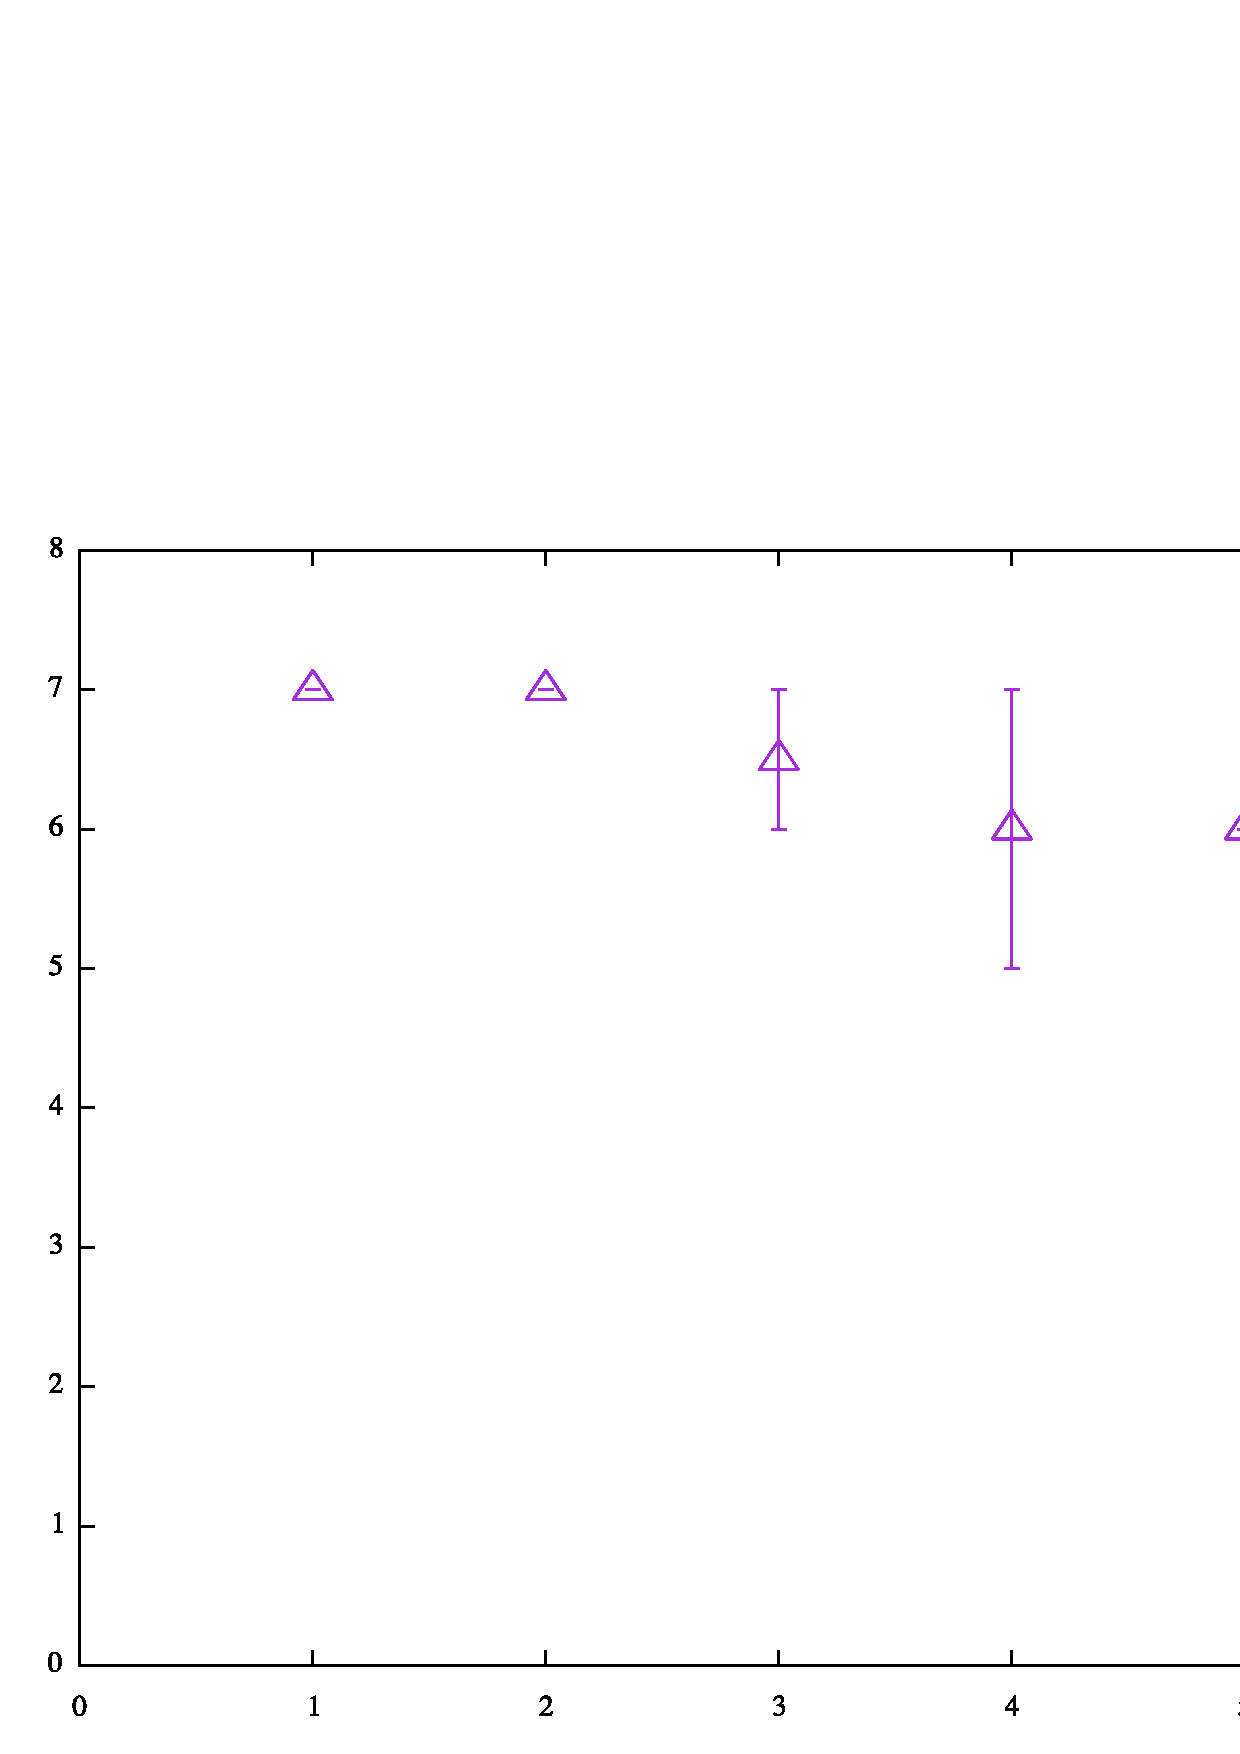
\includegraphics[width=0.9\linewidth]{assets/img/experiment_result.png}
		\caption{評価実験結果プロット}
		\label{graph:experiment_result}
	\end{center}
\end{figure}

\subsubsection{(質問1)ミッションの作成はどちらが操作しやすかったですか}
ゴオルシェアではミッション作成画面で入力項目が多すぎてわかりにくいという声が多く,
ミッションフォレストでは入力項目が少なく明確なので使いやすいという意見があった.

\subsubsection{(質問2)タスクの作成はどちらが操作しやすかったですか}
ゴオルシェアではタスクを作成するたびに画面遷移が発生していたのに対し,
ミッションフォレストでは画面遷移なしにさくさく使えるので使いやすいという意見があった.

\subsubsection{(質問3)画面上のUI構成はどちらがわかりやすかったですか}
ゴオルシェアではボタンやメニューが多く煩雑だが,
ミッションフォレストは今時のUIでシンプルだという意見があった.

\subsubsection{(質問4)どちらのツリー表示が見やすかったですか}
ゴオルシェアではタスクが丸でしか表示されないが,
ミッションフォレストではタスク名も表示されるので見やすいという意見があった.

\subsubsection{(質問5)軽快な動きをするのはどちらでしたか}
ゴオルシェアでは画面遷移のたびに待ち時間があったが,
ミッションフォレストでは画面遷移がないので待ち時間が短いという意見があった.

\subsubsection{(質問6)今後どちらのシステムを使いたいですか}
タスクの作りやすさとツリーの見やすさから,ミッションフォレストを使いたいという意見が多かった.

\cleardoublepage

% 第7章 まとめ
%!TEX root = ../../main.tex
\chapter{まとめ}

\section{本研究の要約}
本稿では,
(1)組織内部の日常的な活動を非公開な目標ツリーとして記録し,
(2)外部発表後にツリー構造の全体もしくは一部のみをLODとしてオープンデータ化可能にする.
さらに,(3)目標ツリーを直感的操作で作成・編集可能にする,
ミッションフォレストの試作について述べた.
実装中であるアクセス制御機構および公開タスクの部分的選択機構については,実装が完了し次第,評価実験を行う予定である.

\section{今後の展望}
今後は,研究室内でのソースコード共有やハッカソンでの使用を想定し,GithubやSlackなどの外部サービスとの連携を可能にする.
また,Web議論システムCOLLAGREE [6]との連携による協働プロセスのアーカイブ化など,より実効性の高い協働支援のできるタスク構造化システムを開発していく予定である.

\cleardoublepage

% 謝辞
%!TEX root = ../../main.tex
\chapter*{謝辞}
\addcontent{謝辞}
本論文を執筆するにあたり,多くの方のご支援ご協力を賜りました.
この場で皆様に感謝の言葉を申し上げたいと思います.

まず,名古屋工業大学大学院 工学研究科 情報工学専攻の白松~俊准教授に厚く御礼申し上げます.
白松教授には日々の研究活動に限らず,研究経験の乏しい私に懇切丁寧にご指導して頂き,数多くの貴重な体験もさせて頂きました.
ここに心より感謝致します.

同研究室の同輩である成瀬~雅人君,西田~拓哉君,山野~太靖君とは特に苦楽を共にしてきました.
その中で,皆の頑張り,励まし,助言に助けられることも多く,充実した日々を過ごすことができました.
ここでみなさんに感謝の意を表しつつ,今後のご活躍をお祈り申し上げます.

最後に,研究活動で帰りが遅くなることもあり迷惑をかけた私を,いつもと変わらず支えてくれた家族に,心より感謝致します.

\vspace*{4.5mm}

\begin{flushright}
思い出で溢れている 白松研究室にて \\
2016年 桜咲く頃に \\
\vspace*{1.8mm}
\end{flushright}

\cleardoublepage

% 参考文献
%!TEX root = ../../main.tex
%修論用
% 参考文献 http://bibdesk.sourceforge.net/manual/BibDesk%20Help_94.html#SEC179 による出力
%以下テンプレ
%<$publications>
%\bibitem{<$citeKey/>}
%<$authors.name.stringByRemovingTeX.@componentsJoinedByComma/>: ``<$fields.Title.stringByRemovingTeX/>,''  <$fields.Journal.stringByRemovingTeX/>. Vol. <$fields.Volume/>,  No. <$fields.Number/>,  pp. <$fields.Pages/>,  <$fields.Year/>.
%<$fields.URL/>
%<$fields.localURL/>
%\begin{quote}
%\end{quote}

%
%</$publications>
\addcontent{参考文献}

\begin{thebibliography}{99}
% メディアについて

\bibitem{hatano2007}
波多野誼余夫(編):"音楽と認知" Vol. 8, 東京大学出版会, (2007)
\begin{quote}
様々な認知研究や音楽理論から音楽心理学を,人間はいかにして音楽を認知するかの研究として捉えて考察をのべている.
\end{quote}

\bibitem{songle}
能動的音楽鑑賞サービスSongle,\url{http://songle.jp/},2015年11月25日アクセス.
\begin{quote}
	能動的音楽鑑賞サービスSongleは動画サイトやネット上にアップロードされた合法的に視聴できる音楽を自動解析し,音楽と一緒にサビ,メロディ,コード,ビートを視覚的に表示させて鑑賞することができる.
\end{quote}

\bibitem{ongakunotomo1979}
音楽之友社:"音楽中辞典" 音楽之友社, (1979)
\begin{quote}
音楽用語の解説・用法を記載した辞典.
\end{quote}

\bibitem{suga2008}
菅道子. "身体表現を取り入れた参加型音楽コンサートの可能性: カノンの理解を目指した 「追いかけっこしよう」 の事例から" 和歌山大学教育学部教育実践総合センター紀要 18 , pp. 121-129, (2008)
\begin{quote}
	音楽理解における身体表現の有効性を小学校低学年を対象とした参加型音楽コンサートの企画・実施を通して検討し,旋律線のてなぞりなどの身体動作が音楽理解を促進することをあげている.
\end{quote}

\bibitem{takahasi2010}
高橋祐樹:"私の研究開発ツール Processing" 映像情報メディア学会誌 Vol. 64, No.12, pp. 1841-1849, (2010)
\begin{quote}
	Processingの説明と,基本的な使い方について述べている.
\end{quote}

\bibitem{nakamura2010}
中村俊介, 竹井将紫: "インタラクティブアート 「KAGURA」 によるワークショップ: 東京ミッドタウン・デザインハブ・キッズウィークにおける子供向けイベントの報告 (B-2 音楽と聴覚のデザイン, 研究発表, 芸術工学会 2010 年度秋期大会 in 浜松)."  芸術工学会誌,  Vol. 54, pp. 48-49, (2010)
\begin{quote}
カメラの前で動いて音声を生成するインタラクティブアート「KAGURA」をデジタルでしかできないインタラクティブな教育コンテンツとして利用しようと考え,東京ミッドタウンで開催された小・中学生向けワークショップで展示したときの報告が書かれている.
\end{quote}

\bibitem{kagura}
KAGURA,\url{http://www.kagura.cc/jp/},2015年11月25日アクセス
\begin{quote}
	Real Senseに対応した身体動作とジェスチャーで操作できる音楽演奏アプリケーション.
\end{quote}

\bibitem{kanke2013}
菅家浩之, 竹川佳成, 寺田努, 塚本昌彦:"Airstic Drum: 実ドラムと仮想ドラムを統合するためのドラムスティックの構築" 情報処理学会論文誌, Vol. 54, No. 4, pp. 1393-1401, (2013)
\begin{quote}
	楽器の運搬と演奏スペースの問題を解決するため,使用頻度の低い打楽器に仮想的なドラムを割り当て加速度センサの閾値から仮想ドラムの叩打と実ドラムの叩打を区別する方法について述べている.
\end{quote}

\bibitem{shiramatsu2015}
Shiramatsu, S., Ozono, T., and Shintani S.: A Computational Model of Tonality Cognition Based on Prime Factor Representation of Frequency Ratios and Its Application. Proc. of SMC 2015, (2015)
\begin{quote}
	調性理解モデルPFG Tonnetzについて述べている.
\end{quote}

\bibitem{behringer10}
Behringer, R. and Elliot, J.: Linking Phys- ical Space with the Riemann Tonnetz for Exploration of Western Tonality, chapter 6, pp. 131–143, Nova Science Publishers, (2010)
\begin{quote}
	1880年にRiemannが発展させたTonnetzを分析し,数式化した.
\end{quote}
%
%\bibitem{hewlett07}
%Hewlett, W., Selfridge-Field, E., and Cor- reia, E.: Tonal Theory for the Digital Age, Vol. 15 of Computing in Musicology, Center for Computer Assisted Research in the Humanities, Stanford University, (2007)
%\begin{quote}
%
%%\end{quote}
%
%\bibitem{tymoczko12}
%Tymoczko, D.: The Generalized Tonnetz, Journal of Music Theory, Vol. 56, No. 1, pp. 1–52, (2012)
%\begin{quote}
%
%\end{quote}

\bibitem{hand_labels}
Intel RealSense SDK 2015 R5 Documentation, \url{https://software.intel.com/sites/landingpage/realsense/camera-sdk/v1.1/documentation/html/index.html?jointtype_pxchanddata.html}, 2016年1月25日アクセス
\begin{quote}
	RealSenseが認識できる関節の種類が載っている.
\end{quote}

\end{thebibliography}

\cleardoublepage

% 付録
\appendix
\documentclass[a4j,12pt,twoside]{jreport}

%%%%%%%%%%%%%%%%%%%%%%%%%%%%%%%%%%%%%%%%%%%%%%%%%
% パッケージ宣言
%%%%%%%%%%%%%%%%%%%%%%%%%%%%%%%%%%%%%%%%%%%%%%%%%
\usepackage{graphicx}
\usepackage{times}
\usepackage{selectp}
\usepackage{epsf}
\usepackage{styles/epsbox}
\usepackage{styles/mediabb}
%\usepackage{styles/boites_exemples}
\usepackage{styles/verbatimfiles}
\usepackage{here}
\usepackage{url}
\usepackage{fancyhdr}
\usepackage{fancyvrb}
\usepackage{styles/algorithm}
\usepackage{styles/algorithmic}
\usepackage{cite}
\usepackage[dvipdfmx, usenames]{color}
\usepackage{colortbl}

\usepackage{ascmac}
\usepackage{amsmath}
\usepackage{amsthm}
\usepackage{amssymb}
\usepackage{latexsym}

\usepackage{styles/thesis}

%%%%%%%%%%%%%%%%%%%%%%%%%%%%%%%%%%%%%%%%%%%%%%%%%
% マクロ定義
%%%%%%%%%%%%%%%%%%%%%%%%%%%%%%%%%%%%%%%%%%%%%%%%%
\newcommand{\argmax}{\mathop{\rm argmax}}
\newcommand{\argmin}{\mathop{\rm argmin}}
\renewcommand{\bibname}{参考文献}

%% myマクロ
%\input{mymacros}

%% マージン設定
%\oddsidemargin=17mm
%\evensidemargin=-4mm

%%%%%%%%%%%%%%%%%%%%%%%%%%%%%%%%%%%%%%%%%%%%%%%%%
% 本文開始
%%%%%%%%%%%%%%%%%%%%%%%%%%%%%%%%%%%%%%%%%%%%%%%%%
\begin{document}
\newtheorem{defi}{Definition}[section]
\newtheorem{thy}{Theorem}[section]

\pagestyle{fancyplain}

%\pagenumbering{roman}

% タイトルページ
\newlength{\oldtextwidth}
\setlength{\oldtextwidth}{\textwidth}
\setlength{\textwidth}{40zw}

\documentclass[a4j,12pt,twoside]{jreport}

%%%%%%%%%%%%%%%%%%%%%%%%%%%%%%%%%%%%%%%%%%%%%%%%%
% パッケージ宣言
%%%%%%%%%%%%%%%%%%%%%%%%%%%%%%%%%%%%%%%%%%%%%%%%%
\usepackage{graphicx}
\usepackage{times}
\usepackage{selectp}
\usepackage{epsf}
\usepackage{styles/epsbox}
\usepackage{styles/mediabb}
%\usepackage{styles/boites_exemples}
\usepackage{styles/verbatimfiles}
\usepackage{here}
\usepackage{url}
\usepackage{fancyhdr}
\usepackage{fancyvrb}
\usepackage{styles/algorithm}
\usepackage{styles/algorithmic}
\usepackage{cite}
\usepackage[dvipdfmx, usenames]{color}
\usepackage{colortbl}

\usepackage{ascmac}
\usepackage{amsmath}
\usepackage{amsthm}
\usepackage{amssymb}
\usepackage{latexsym}

\usepackage{styles/thesis}

%%%%%%%%%%%%%%%%%%%%%%%%%%%%%%%%%%%%%%%%%%%%%%%%%
% マクロ定義
%%%%%%%%%%%%%%%%%%%%%%%%%%%%%%%%%%%%%%%%%%%%%%%%%
\newcommand{\argmax}{\mathop{\rm argmax}}
\newcommand{\argmin}{\mathop{\rm argmin}}
\renewcommand{\bibname}{参考文献}

%% myマクロ
%\input{mymacros}

%% マージン設定
%\oddsidemargin=17mm
%\evensidemargin=-4mm

%%%%%%%%%%%%%%%%%%%%%%%%%%%%%%%%%%%%%%%%%%%%%%%%%
% 本文開始
%%%%%%%%%%%%%%%%%%%%%%%%%%%%%%%%%%%%%%%%%%%%%%%%%
\begin{document}
\newtheorem{defi}{Definition}[section]
\newtheorem{thy}{Theorem}[section]

\pagestyle{fancyplain}

%\pagenumbering{roman}

% タイトルページ
\newlength{\oldtextwidth}
\setlength{\oldtextwidth}{\textwidth}
\setlength{\textwidth}{40zw}

\documentclass[a4j,12pt,twoside]{jreport}

%%%%%%%%%%%%%%%%%%%%%%%%%%%%%%%%%%%%%%%%%%%%%%%%%
% パッケージ宣言
%%%%%%%%%%%%%%%%%%%%%%%%%%%%%%%%%%%%%%%%%%%%%%%%%
\usepackage{graphicx}
\usepackage{times}
\usepackage{selectp}
\usepackage{epsf}
\usepackage{styles/epsbox}
\usepackage{styles/mediabb}
%\usepackage{styles/boites_exemples}
\usepackage{styles/verbatimfiles}
\usepackage{here}
\usepackage{url}
\usepackage{fancyhdr}
\usepackage{fancyvrb}
\usepackage{styles/algorithm}
\usepackage{styles/algorithmic}
\usepackage{cite}
\usepackage[dvipdfmx, usenames]{color}
\usepackage{colortbl}

\usepackage{ascmac}
\usepackage{amsmath}
\usepackage{amsthm}
\usepackage{amssymb}
\usepackage{latexsym}

\usepackage{styles/thesis}

%%%%%%%%%%%%%%%%%%%%%%%%%%%%%%%%%%%%%%%%%%%%%%%%%
% マクロ定義
%%%%%%%%%%%%%%%%%%%%%%%%%%%%%%%%%%%%%%%%%%%%%%%%%
\newcommand{\argmax}{\mathop{\rm argmax}}
\newcommand{\argmin}{\mathop{\rm argmin}}
\renewcommand{\bibname}{参考文献}

%% myマクロ
%\input{mymacros}

%% マージン設定
%\oddsidemargin=17mm
%\evensidemargin=-4mm

%%%%%%%%%%%%%%%%%%%%%%%%%%%%%%%%%%%%%%%%%%%%%%%%%
% 本文開始
%%%%%%%%%%%%%%%%%%%%%%%%%%%%%%%%%%%%%%%%%%%%%%%%%
\begin{document}
\newtheorem{defi}{Definition}[section]
\newtheorem{thy}{Theorem}[section]

\pagestyle{fancyplain}

%\pagenumbering{roman}

% タイトルページ
\newlength{\oldtextwidth}
\setlength{\oldtextwidth}{\textwidth}
\setlength{\textwidth}{40zw}

\include{components/_title/main}
\cleardoublepage

% タイトル以降用パラメータ
\setlength{\oddsidemargin}{17mm}
\setlength{\evensidemargin}{-4mm}
\setlength{\textwidth}{\oldtextwidth}

\cleardoublepage

%ここからページ数開始
\pagenumbering{arabic}

% アブストラクト
\cleardoublepage
%\pagenumbering{roman}
\include{components/00.Abstract/main}
% \include{part/00.Abstract/abstract-e}
\cleardoublepage

% 目次
\include{components/_contents/main}
\cleardoublepage

% 序章
\include{components/01.Introduction/main}
\cleardoublepage

% 関連研究
\include{components/02.RelatedWorks/main}
\cleardoublepage

% 期間毎の特徴語抽出手法
\include{components/03.Interface/main}
\cleardoublepage

% タイムスケールを考慮した時系列的話題追跡
\include{components/04.LOD/main}
\cleardoublepage

% ツイートの探索的閲覧支援システムの実装
\include{components/05.Recommendation/main}
\cleardoublepage

% 評価・考察
\include{components/06.Evaluation/main}
\cleardoublepage

% まとめ
\include{components/07.Conclusion/main}
\cleardoublepage

% 謝辞
\include{components/08.Acknowledgement/main}
\cleardoublepage

% 参考文献
\include{components/09.Bibliography/main}
\cleardoublepage

\appendix
\include{components/10.Appendix/IPSJ/main}

\cleardoublepage
\include{components/_title/main}

\end{document}

\cleardoublepage

% タイトル以降用パラメータ
\setlength{\oddsidemargin}{17mm}
\setlength{\evensidemargin}{-4mm}
\setlength{\textwidth}{\oldtextwidth}

\cleardoublepage

%ここからページ数開始
\pagenumbering{arabic}

% アブストラクト
\cleardoublepage
%\pagenumbering{roman}
%!TEX root = ../../main.tex
\chapter*{論文要旨}
\label{chap0}
\addcontent{論文要旨}
本研究ではこれまで,公益活動やシビックテックといった分野を対象とし,公共圏で目標を共有するWebシステム「ゴオルシェア」を開発・運営してきた.
しかし,非公開な組織内部の活動には適していない問題があった.
新システム「MissionForest」では,組織内部の日常的な活動を非公開な目標ツリーとして記録し,外部発表後にツリー構造の一部をオープンデータ化可能にする.
さらに,目標ツリーを直感的操作で作成・編集可能にする.
これにより,組織内部の日常的な活動から組織外部との協働までをサポートする.

% \chapter*{Abstract}
\label{chap:Abstract-e}
\addcontent{Abstract}

Because of the spread of smartphones and the growth of the network technology, use of the social networking/micro-blogging service Twitter has spread widely. 
%スマートフォンの普及やネットワーク技術の発展により,Twitter などの SNS は 急速な成長を遂げた.
Social media such as tweets is attracting attention to its information value to know what they are doing and what they are thinking. 
%個人が用意に情報を発信できるため,一般の人々が何をして いるのか,何を思っているのかなど情報源としての価値も注目されつつあるそ
In recent years, a demand of society for analyzing topics in Twitter has been increasing.
 %そのような背景に伴い,近年,Twitter における話題分析のための技術に対する社会的要請は高まってきている.
However, so far, a usage scenario where users hark back to past event through browsing past timeline of Twitter has not been considered. 
%しかしながら,従来,過去のタイムラインをアーカ イブ化して振り返るような使い方は想定されていなかった
Therefore, we proposed a method of exploratory browsing for the past tweets set about a specific topic. 
%そこで,本研究では, ある話題に関する過去のツイート群における探索的閲覧手法を提案する

For a lot of tweets,  users cannot remember contents of the past tweets. It is difficult to determine an appropriate query for searching past tweets.
%大量に存在するツイート集合において,ユーザは過去にあった大量のツイートの内容を 知るはずもなく,何をクエリとして検索すればいいのか分からない.
In order to grasp the background of a specific topic, it is desirable to know time-series flows of features of tweets about the topic such as what events make trends of tweets changed.
%特定の話題 の背景を把握するためには,その話題に関するツイートの傾向がどのような流れ で移り変わっていったか,どのような出来事がツイートの傾向を変えたかという 時系列的な流れを知ることが望ましい.
Visualizing topics using a burst detection for Twitter is one of the researches about exploratory browsing for tweets.  
%ツイートに対する探索的閲覧の研究の中 でもバースト検出を利用したトピックの可視化などがあるが,
However, the method extracts only features from tweets in the burst period. In other words, it cannot extract features from tweets in all time.   
%従来の手法では盛り上がりのあった期間の特徴のみを抽出し,それ以外の期間の特徴が欠けてしまう
Presenting  features in only a particular time span, users cannot grasp detail information such as the changes of features in the time span.
%またある固定された区間の特徴のみをユーザに提示するだけでは,その区間 内の特徴の推移など,詳細な情報を把握することができない.
For users who lack knowledge about the retrieval object, these are not satisfied about the comprehensiveness of exploratory browsing. 
%検索対象に関する 知識の乏しいユーザにとって,これらは探索的閲覧における網羅性を満たしてい ない.

To solve these problems, we implemented an exploratory tweets browsing system which can extract feature terms from each time period, in a day or in a week or in a month,  using the statistical method combining Information Gain and Pointwise Mutual Information.
%そのために,本研究では,日,週,月の異なるタイムスケール毎にツイート を分割し,それぞれの期間内ツイート群から,統計的手法である情報利得と自己 相互情報量を用いた特徴語抽出を実現,
The system enables users to browse overview of tweets changing time scale and figure out the features of tweets along time-series.
%ユーザが動的にタイムスケールを調整 しながら閲覧することで,時系列に沿ったツイートの探索が可能な探索的閲覧支 援システムを開発した
We proposed Bias-Penalized Information Gain which can exclude inadequate terms that a specific user has frequently posted. We showed the effectiveness of the method by experimental results.
%また,期間の特徴語として不適切な語を除外するための バイアス罰則付き情報利得を提案し,実験からその有効性を示した.
Moreover, we confirmed that the exploratory browsing method we proposed is effective in recognizing a causal relationship between events and  opinions in a lot of past tweets by the experiment of tracking topics using the system.
%さらに,本 システムを利用した話題追跡の実験結果から,本研究での探索的閲覧手法が,過 去の大量のツイート群に対し出来事や意見などの時系列的な因果関係の把握に有 効であることを確認した.


\cleardoublepage

% 目次
\documentclass[a4j,12pt,twoside]{jreport}

%%%%%%%%%%%%%%%%%%%%%%%%%%%%%%%%%%%%%%%%%%%%%%%%%
% パッケージ宣言
%%%%%%%%%%%%%%%%%%%%%%%%%%%%%%%%%%%%%%%%%%%%%%%%%
\usepackage{graphicx}
\usepackage{times}
\usepackage{selectp}
\usepackage{epsf}
\usepackage{styles/epsbox}
\usepackage{styles/mediabb}
%\usepackage{styles/boites_exemples}
\usepackage{styles/verbatimfiles}
\usepackage{here}
\usepackage{url}
\usepackage{fancyhdr}
\usepackage{fancyvrb}
\usepackage{styles/algorithm}
\usepackage{styles/algorithmic}
\usepackage{cite}
\usepackage[dvipdfmx, usenames]{color}
\usepackage{colortbl}

\usepackage{ascmac}
\usepackage{amsmath}
\usepackage{amsthm}
\usepackage{amssymb}
\usepackage{latexsym}

\usepackage{styles/thesis}

%%%%%%%%%%%%%%%%%%%%%%%%%%%%%%%%%%%%%%%%%%%%%%%%%
% マクロ定義
%%%%%%%%%%%%%%%%%%%%%%%%%%%%%%%%%%%%%%%%%%%%%%%%%
\newcommand{\argmax}{\mathop{\rm argmax}}
\newcommand{\argmin}{\mathop{\rm argmin}}
\renewcommand{\bibname}{参考文献}

%% myマクロ
%\input{mymacros}

%% マージン設定
%\oddsidemargin=17mm
%\evensidemargin=-4mm

%%%%%%%%%%%%%%%%%%%%%%%%%%%%%%%%%%%%%%%%%%%%%%%%%
% 本文開始
%%%%%%%%%%%%%%%%%%%%%%%%%%%%%%%%%%%%%%%%%%%%%%%%%
\begin{document}
\newtheorem{defi}{Definition}[section]
\newtheorem{thy}{Theorem}[section]

\pagestyle{fancyplain}

%\pagenumbering{roman}

% タイトルページ
\newlength{\oldtextwidth}
\setlength{\oldtextwidth}{\textwidth}
\setlength{\textwidth}{40zw}

\include{components/_title/main}
\cleardoublepage

% タイトル以降用パラメータ
\setlength{\oddsidemargin}{17mm}
\setlength{\evensidemargin}{-4mm}
\setlength{\textwidth}{\oldtextwidth}

\cleardoublepage

%ここからページ数開始
\pagenumbering{arabic}

% アブストラクト
\cleardoublepage
%\pagenumbering{roman}
\include{components/00.Abstract/main}
% \include{part/00.Abstract/abstract-e}
\cleardoublepage

% 目次
\include{components/_contents/main}
\cleardoublepage

% 序章
\include{components/01.Introduction/main}
\cleardoublepage

% 関連研究
\include{components/02.RelatedWorks/main}
\cleardoublepage

% 期間毎の特徴語抽出手法
\include{components/03.Interface/main}
\cleardoublepage

% タイムスケールを考慮した時系列的話題追跡
\include{components/04.LOD/main}
\cleardoublepage

% ツイートの探索的閲覧支援システムの実装
\include{components/05.Recommendation/main}
\cleardoublepage

% 評価・考察
\include{components/06.Evaluation/main}
\cleardoublepage

% まとめ
\include{components/07.Conclusion/main}
\cleardoublepage

% 謝辞
\include{components/08.Acknowledgement/main}
\cleardoublepage

% 参考文献
\include{components/09.Bibliography/main}
\cleardoublepage

\appendix
\include{components/10.Appendix/IPSJ/main}

\cleardoublepage
\include{components/_title/main}

\end{document}

\cleardoublepage

% 序章
%!TEX root = ../../main.tex
\chapter{序論}
\label{chap:intro}

\section{本研究の背景}
音楽知識や音楽経験に乏しい人が音楽によるインタラクションを試みる際,調性感を損なわない音を発して参加することは非常に困難である.
実際に音楽未経験者が自由にかつ能動的に音楽インタラクションに参加する場合として,
地域社会振興のために開催される音楽イベント,アーティストのコンサート,などが考えられる.
従来,音楽経験の乏しい人がそのようなパフォーマンスに参加する手段は手拍子や掛け声,リズムに合わせて体を動かす程度のことに限られている,
波多野\cite{hatano2007}は旋律歌唱能力の発達過程や旋律聴取の認知的処理における3つの処理側面として,図\ref{img:hatano}に示すように,(1)リズム(rhythm),(2)旋律線(pitch contour),(3)調性(tonality)があるとしている.
(2)の旋律線とは音高の上がり下がりの運動パターンのことであり,初心者でもリズムやおおまかになら音が上がったか下がったかは比較的理解しやすい.(3)の調性とは文献\cite{ongakunotomo1979}によれば,広義には「支配的な中心音を有する音楽系」を指し,狭義には「長短調いずれかの主和音をもつ和声的な音楽系」を指す.調性は中心音,長調/短調,音階,和音などから説明され,音楽初心者が音楽について学ぼうとする場合,調性を理解することは最も大きな障害のひとつである.
よって調性は音楽未経験者が音楽活動を行おうとする際,苦手意識を持たれる原因となる.
この調性に関する知識の無さが引き起こす問題点を解決することで,誰でもより充実した音楽活動をすることが容易になると考えた.

\begin{figure}[t]
	\begin{center}
		\includegraphics[width=0.9\linewidth]{assets/img/hatano.png}
		 \caption{旋律歌唱や旋律聴取の認知的処理における3つの処理側面}
		\label{img:hatano}
	\end{center}
\end{figure}
\section{本研究の目的}
本研究の目的は,ユーザーが直感的に操作できるように比較的知識を必要としないリズムと旋律線を身体動作で入力すれば,システムの音高補正により背景で流れている楽曲との調性の制約(以下,調性制約)に従って背景楽曲と協和を満たす演奏音を出力することで,音楽知識がなくても合奏ができる演奏インタフェースの実現である. 菅\cite{suga2008}は旋律線の手なぞりなどの身体動作が音楽理解を促進する方法として有効であるとしている.そのため旋律線の入力手段として身体動作を用いることは適切である.
本研究完成時には調性感を共有した演奏参加が可能になると期待される.コンサート会場で演奏される実楽曲の調や旋法と同期させた使い方を考えると,ステージ上のアーティストと聴衆のインタラクションのあり方を変える可能性があり,さらに,学校・保育施設での情操教育や福祉施設でのリハビリテーションにも活用できる可能性があり,幼児,児童,高齢者などのQOL向上に繋がると期待される.
また,旋律線とリズムを身体動作で入力することにより,ユーザーは演奏のための楽器を持ち運ぶ必要がなくなるため,演奏場所への移動距離や,スペースの制約に縛られることがない.
その操作性と音高の決定手法においていくつかの問題点ある.本研究ではそれらの問題を
(1)直感的な身体動作による旋律線やタイミング,音の種類などの入力手法.(2)演奏音の発音可能な音高範囲の指定.(3)調性制約の生成.の3つの課題として設定した.
\subsection{システム構成}
本システムのシステム構成を図\ref{img:sys_const}に示す.
まず,ユーザーはモーションセンサーの前でリズムと旋律線を身体動作で入力する.本研究ではモーションセンサーはIntel RealSense 3D Camera\footnote{http://www.intel.co.jp/content/www/jp/ja/architecture-and-technology/realsense-overview.html} (以下,RealSense)を使用した,RealSenseは手指の情報とジェスチャーを検出し,認識結果を本研究で実装する合奏支援システムに渡す.システム内部ではジェスチャーによるイベント切り替えや,手の座標とあらかじめ用意しておいた調性制約から背景楽曲と不協和音にならない演奏音を出力する.
\begin{figure}[t]
	\begin{center}
		\includegraphics[width=0.9\linewidth]{assets/img/system_configuration_diagram.png}
		\caption{システム構成図}
		\label{img:sys_const}
	\end{center}
\end{figure}
\section{本論文の構成}
本論文の構成を以下に示す.第2章では関連研究や関連システムと本研究の動作・開発環境について述べる.第3章では直感的な身体動作とリズムの入力手法について述べる.第4章では演奏音の発音可能な音高範囲の指定について述べる.第5章では調性制約の生成について述べる,第6章では前章までで述べたシステムの評価実験の結果をまとめ,第7章で本研究をまとめる.

\cleardoublepage

% 関連研究
%!TEX root = ../../main.tex
\chapter{動作・開発環境と関連研究}
\section{動作・開発環境}
本研究の動作・開発環境について述べる.

\subsection{Intel RealSense 3D Camera}
旋律線とリズムの直感的な入力手段として使用した.RealSenseは手指やジェスチャー,顔の部位や表情,心拍や音声,対象物の奥行きなどを認識することができる.さらに,今後各国の主要PCメーカーがRealSenseを内蔵したPCを発売することに賛同している.従来,Kinect\footnote{http://www.xbox.com/ja-JP/kinect}をはじめとするモーションセンサ類を使用するにはわざわざデバイスを購入しなければならず,モーションセンサ類の存在を知らなかったり,存在を知っていても新たにデバイスを用意する手間や安価であっても購入の費用を嫌う人は一部のユーザーが使うものという認識であった.RealSense搭載PCの増加やWindows Helloなどモーションセンサでの開発経験のない一般ユーザーでも,容易に手に入ったり認知することができるRealSenseはその普及度においても期待されているデバイスである.

\subsection{Processing}
本システムの実装には,RealSense SDKを扱うことができ,画像や音声を比較的容易に行うことができるプログラミング言語Processingを用いる.Processing\footnote{https://www.processing.org/}は,MIT(Massachusetts Institute of Technology)メディアラボに所属していたCasey ReasとBen Fryによって開発された,視覚芸術のためのプログラミング教育ように作られたJavaをベースにした開発環境である.\cite{takahasi2010}
\section{関連研究}
本研究と関連のある研究やシステムを紹介する.

\subsection{Songle}
Songle\cite{songle}とは,音楽をサビ,メロディ,コード,ビートなどの構造を表示しながら鑑賞できるサービスで,ピアプロ\footnote{http://piapro.jp/}やSoundCloud\footnote{https://soundcloud.com/}の楽曲ページ,ニコニコ動画\footnote{http://www.nicovideo.jp/}やYouTube\footnote{https://www.youtube.com/}などにアップロードされている合法的に視聴可能な楽曲を音楽理解技術により自動解析しAメロ・Bメロ・サビといった繰り返し構造や、ビートの位置・コード進行・ボーカルの音高などを自動的に解析して見ることができる.さらにSongle上では複数のユーザでコンピュータの自動解析による誤差を訂正することで,解析結果の精度を高めている.また,Songle解析結果をJavaScriptから操作し,WEB上で利用するためのSongle Widget API\footnote{https://widget.songle.jp/}を用いることによって解析結果をJSONファイルとして参照することができる.

\subsection{KAGURA}
中村ら\cite{nakamura2010}はRealSenseを利用した音楽演奏アプリKAGURA\cite{kagura}を開発した.KAGURAはRealSenseを使用することによりRealSenseの特徴であるジェスチャー認識機能を利用し,身体動作で音の高さを,ジェスチャーで細かい設定や操作を指定することができる.出力される音は不協和音にならないようになっているため,適当に体を動かしたり,音楽演奏経験のない人でも音楽を演奏することができる.
また,KAGURAには録画機能とYouTubeへのアップロード機能が付いているため,気に入った演奏をすぐにインターネット上に公開することも容易に行えるようになっている.
\subsection{Airstic Drum}
菅家ら\cite{kanke2013}は,物理的に打面のあるドラム楽器(以下,実ドラム)の問題点を解決するために,実ドラムの補助として使用頻度の少ない打楽器に対して仮想ドラムを適用することで実ドラムと仮想ドラムの両方の利点を持ったAirstic Drumを設計した.この仮想ドラムの実装は無線通信機能を持つ加速度センサを搭載したドラムスティックから得られる加速度,角速度に閾値を設定し音の出力タイミングとしている.具体的には,加速度が設定された閾値(以下,基準強度)を超え,再び基準強度を下回るまでの経過時間の実ドラムと仮想ドラムの違いを識別して仮想ドラムの叩打タイミングとしている.また,仮想ドラムの叩打と演奏音の出力タイミングの時間差を測定するため,60bpm,90bpm,120bpmのテンポでメトロノームに合わせて仮想ドラムの叩打を繰り返し,メトロノームのクリック音とMIDI音源にメッセージが送信されるタイミングの時間差を計測した.

\subsection{調性理解モデルPFG Tonnetz}
白松ら\cite{shiramatsu2015}は調性理解モデルPFG Tonnetz (Prime Factor-based Generalized Tonnetz)を考案した.ある調の主音の周波数と協和音程の周波数比は,

\begin{align}
f=\Bigl(\prod_{pはn以下の素数} p^{(z_p)}\Bigr)\cdot f_{\rm tonic} ~~(z_pは整数)
\end{align}

のような素数の積で表すことができる.白松らは$n=5$と置いた上で,オクターブ隔たった音は音楽的に等価であることを考慮し,2の指数$z_2$軸をなくして$z_{3}z_{5}$平面へ投影すると,

\begin{figure}[t]
\begin{center}
	\includegraphics[width=0.9\linewidth]{./assets/pfg-tonnetz.png}
	\caption{調性理解モデル PFG Tonnetz (5-limit)\cite{shiramatsu2015}}
	\label{img:pfg-tonnetz}
\end{center}
\end{figure}
図\ref{img:pfg-tonnetz}のように$z_3z_5$平面に配置される.この平面上の根音$(a,b)$に対して以下のような整数格子点列$\mathrm{chord}(a,b,\delta,m)$を考える.

\begin{align}
\mathrm{chord}(a,b,\delta,m)=\bigl[(a,b)+\sum_{i=0}^k \delta(i)\bigr]_{k=0,1,\cdots,m} \label{eq:code}\\
\delta_{\rm maj}(i)=\begin{cases}(0,1)&(iが奇数のとき)\\(1,-1)&(iが偶数のとき)\end{cases} \label{eq:maj}\\
\delta_{\rm min}(i)=\begin{cases}(1,-1)&(iが奇数のとき)\\(0,1)&(iが偶数のとき) \label{eq:min}\end{cases}
\end{align}

根音$(a,b)$を調の主音$(0,0)$で置き換えて考えると,明るい長音階の構成音(I, II, III, IV, V, VI, VII)が原点の上側$0 \leq z_5 \leq 1$に分布し,暗い短音階の構成音(I, II, \#II, IV, V, \#V, \#VI)が原点の下側$-1 \leq z_5 \leq 0$に分布するのが見て取れる.

このモデルは,音名,階名,コード名のようなシンボルを前提としては用いておらず,周波数比に基づく認知的原理のみから導かれる.まとめると,導出の過程で現れた以下の表現形式は,上記の認知的原理および導出されたモデルの観察から自然に導かれたものである.

\begin{itemize}
\item 整数格子点$(z_3, z_5)$: 音階の構成音,階名
\item 三角形$\bigl[(a,b)$, $(a,b+1)$, $(a+1,b)\bigr]$:\\
~~~ 整数格子点$(a,b)$を根音とする長三和音
\item 三角形$\bigl[(a,b)$, $(a+1,b-1)$, $(a+1,b)\bigr]$:\\
~~~ $(a,b)$を根音とする短三和音
\item 整数格子点列$\mathrm{chord}(a,b,\delta_{\rm maj},m)$:\\
~~~ $(a,b)$を根音とする長和音
\item 整数格子点列$\mathrm{chord}(a,b,\delta_{\rm min},m)$:\\
~~~ $(a,b)$を根音とする短和音
\end{itemize}

このPFG Tonnetzは数学者Leonhard Eulerが1739年に考案した調性理解モデルをもとに.
音楽学者Hugo Riemannが1880年に発展させたTonnetzというモデルに似ている
Tonnetzは1980年代以降,数学的に定式化された新リーマン理論(NeoRiemannian theory)へと発展し,様々な拡張が行われた\cite{behringer10}%\cite{tymoczko12}
が基本的には図\ref{img:euler},図\ref{img:riemann}のように音名同士を繋いだモデルであり,調の主音は表現できていない.
\begin{figure}[t]
	\begin{center}
		\includegraphics[width=0.9\linewidth]{./assets/Eulers_tonnetz.png}
		\caption{Eulerの調性理解モデル\cite{shiramatsu2015}}
		\label{img:euler}
	\end{center}
\end{figure}
\begin{figure}[t]
	\begin{center}
		\includegraphics[width=0.9\linewidth]{./assets/tonnetz_vertical.png}
		\caption{Riemannの調性理解モデル\cite{shiramatsu2015}}
		\label{img:riemann}
	\end{center}
\end{figure}

\cleardoublepage

% 期間毎の特徴語抽出手法
\documentclass[a4j,12pt,twoside]{jreport}

%%%%%%%%%%%%%%%%%%%%%%%%%%%%%%%%%%%%%%%%%%%%%%%%%
% パッケージ宣言
%%%%%%%%%%%%%%%%%%%%%%%%%%%%%%%%%%%%%%%%%%%%%%%%%
\usepackage{graphicx}
\usepackage{times}
\usepackage{selectp}
\usepackage{epsf}
\usepackage{styles/epsbox}
\usepackage{styles/mediabb}
%\usepackage{styles/boites_exemples}
\usepackage{styles/verbatimfiles}
\usepackage{here}
\usepackage{url}
\usepackage{fancyhdr}
\usepackage{fancyvrb}
\usepackage{styles/algorithm}
\usepackage{styles/algorithmic}
\usepackage{cite}
\usepackage[dvipdfmx, usenames]{color}
\usepackage{colortbl}

\usepackage{ascmac}
\usepackage{amsmath}
\usepackage{amsthm}
\usepackage{amssymb}
\usepackage{latexsym}

\usepackage{styles/thesis}

%%%%%%%%%%%%%%%%%%%%%%%%%%%%%%%%%%%%%%%%%%%%%%%%%
% マクロ定義
%%%%%%%%%%%%%%%%%%%%%%%%%%%%%%%%%%%%%%%%%%%%%%%%%
\newcommand{\argmax}{\mathop{\rm argmax}}
\newcommand{\argmin}{\mathop{\rm argmin}}
\renewcommand{\bibname}{参考文献}

%% myマクロ
%\input{mymacros}

%% マージン設定
%\oddsidemargin=17mm
%\evensidemargin=-4mm

%%%%%%%%%%%%%%%%%%%%%%%%%%%%%%%%%%%%%%%%%%%%%%%%%
% 本文開始
%%%%%%%%%%%%%%%%%%%%%%%%%%%%%%%%%%%%%%%%%%%%%%%%%
\begin{document}
\newtheorem{defi}{Definition}[section]
\newtheorem{thy}{Theorem}[section]

\pagestyle{fancyplain}

%\pagenumbering{roman}

% タイトルページ
\newlength{\oldtextwidth}
\setlength{\oldtextwidth}{\textwidth}
\setlength{\textwidth}{40zw}

\include{components/_title/main}
\cleardoublepage

% タイトル以降用パラメータ
\setlength{\oddsidemargin}{17mm}
\setlength{\evensidemargin}{-4mm}
\setlength{\textwidth}{\oldtextwidth}

\cleardoublepage

%ここからページ数開始
\pagenumbering{arabic}

% アブストラクト
\cleardoublepage
%\pagenumbering{roman}
\include{components/00.Abstract/main}
% \include{part/00.Abstract/abstract-e}
\cleardoublepage

% 目次
\include{components/_contents/main}
\cleardoublepage

% 序章
\include{components/01.Introduction/main}
\cleardoublepage

% 関連研究
\include{components/02.RelatedWorks/main}
\cleardoublepage

% 期間毎の特徴語抽出手法
\include{components/03.Interface/main}
\cleardoublepage

% タイムスケールを考慮した時系列的話題追跡
\include{components/04.LOD/main}
\cleardoublepage

% ツイートの探索的閲覧支援システムの実装
\include{components/05.Recommendation/main}
\cleardoublepage

% 評価・考察
\include{components/06.Evaluation/main}
\cleardoublepage

% まとめ
\include{components/07.Conclusion/main}
\cleardoublepage

% 謝辞
\include{components/08.Acknowledgement/main}
\cleardoublepage

% 参考文献
\include{components/09.Bibliography/main}
\cleardoublepage

\appendix
\include{components/10.Appendix/IPSJ/main}

\cleardoublepage
\include{components/_title/main}

\end{document}

\cleardoublepage

% タイムスケールを考慮した時系列的話題追跡
\documentclass[a4j,12pt,twoside]{jreport}

%%%%%%%%%%%%%%%%%%%%%%%%%%%%%%%%%%%%%%%%%%%%%%%%%
% パッケージ宣言
%%%%%%%%%%%%%%%%%%%%%%%%%%%%%%%%%%%%%%%%%%%%%%%%%
\usepackage{graphicx}
\usepackage{times}
\usepackage{selectp}
\usepackage{epsf}
\usepackage{styles/epsbox}
\usepackage{styles/mediabb}
%\usepackage{styles/boites_exemples}
\usepackage{styles/verbatimfiles}
\usepackage{here}
\usepackage{url}
\usepackage{fancyhdr}
\usepackage{fancyvrb}
\usepackage{styles/algorithm}
\usepackage{styles/algorithmic}
\usepackage{cite}
\usepackage[dvipdfmx, usenames]{color}
\usepackage{colortbl}

\usepackage{ascmac}
\usepackage{amsmath}
\usepackage{amsthm}
\usepackage{amssymb}
\usepackage{latexsym}

\usepackage{styles/thesis}

%%%%%%%%%%%%%%%%%%%%%%%%%%%%%%%%%%%%%%%%%%%%%%%%%
% マクロ定義
%%%%%%%%%%%%%%%%%%%%%%%%%%%%%%%%%%%%%%%%%%%%%%%%%
\newcommand{\argmax}{\mathop{\rm argmax}}
\newcommand{\argmin}{\mathop{\rm argmin}}
\renewcommand{\bibname}{参考文献}

%% myマクロ
%\input{mymacros}

%% マージン設定
%\oddsidemargin=17mm
%\evensidemargin=-4mm

%%%%%%%%%%%%%%%%%%%%%%%%%%%%%%%%%%%%%%%%%%%%%%%%%
% 本文開始
%%%%%%%%%%%%%%%%%%%%%%%%%%%%%%%%%%%%%%%%%%%%%%%%%
\begin{document}
\newtheorem{defi}{Definition}[section]
\newtheorem{thy}{Theorem}[section]

\pagestyle{fancyplain}

%\pagenumbering{roman}

% タイトルページ
\newlength{\oldtextwidth}
\setlength{\oldtextwidth}{\textwidth}
\setlength{\textwidth}{40zw}

\include{components/_title/main}
\cleardoublepage

% タイトル以降用パラメータ
\setlength{\oddsidemargin}{17mm}
\setlength{\evensidemargin}{-4mm}
\setlength{\textwidth}{\oldtextwidth}

\cleardoublepage

%ここからページ数開始
\pagenumbering{arabic}

% アブストラクト
\cleardoublepage
%\pagenumbering{roman}
\include{components/00.Abstract/main}
% \include{part/00.Abstract/abstract-e}
\cleardoublepage

% 目次
\include{components/_contents/main}
\cleardoublepage

% 序章
\include{components/01.Introduction/main}
\cleardoublepage

% 関連研究
\include{components/02.RelatedWorks/main}
\cleardoublepage

% 期間毎の特徴語抽出手法
\include{components/03.Interface/main}
\cleardoublepage

% タイムスケールを考慮した時系列的話題追跡
\include{components/04.LOD/main}
\cleardoublepage

% ツイートの探索的閲覧支援システムの実装
\include{components/05.Recommendation/main}
\cleardoublepage

% 評価・考察
\include{components/06.Evaluation/main}
\cleardoublepage

% まとめ
\include{components/07.Conclusion/main}
\cleardoublepage

% 謝辞
\include{components/08.Acknowledgement/main}
\cleardoublepage

% 参考文献
\include{components/09.Bibliography/main}
\cleardoublepage

\appendix
\include{components/10.Appendix/IPSJ/main}

\cleardoublepage
\include{components/_title/main}

\end{document}

\cleardoublepage

% ツイートの探索的閲覧支援システムの実装
\documentclass[a4j,12pt,twoside]{jreport}

%%%%%%%%%%%%%%%%%%%%%%%%%%%%%%%%%%%%%%%%%%%%%%%%%
% パッケージ宣言
%%%%%%%%%%%%%%%%%%%%%%%%%%%%%%%%%%%%%%%%%%%%%%%%%
\usepackage{graphicx}
\usepackage{times}
\usepackage{selectp}
\usepackage{epsf}
\usepackage{styles/epsbox}
\usepackage{styles/mediabb}
%\usepackage{styles/boites_exemples}
\usepackage{styles/verbatimfiles}
\usepackage{here}
\usepackage{url}
\usepackage{fancyhdr}
\usepackage{fancyvrb}
\usepackage{styles/algorithm}
\usepackage{styles/algorithmic}
\usepackage{cite}
\usepackage[dvipdfmx, usenames]{color}
\usepackage{colortbl}

\usepackage{ascmac}
\usepackage{amsmath}
\usepackage{amsthm}
\usepackage{amssymb}
\usepackage{latexsym}

\usepackage{styles/thesis}

%%%%%%%%%%%%%%%%%%%%%%%%%%%%%%%%%%%%%%%%%%%%%%%%%
% マクロ定義
%%%%%%%%%%%%%%%%%%%%%%%%%%%%%%%%%%%%%%%%%%%%%%%%%
\newcommand{\argmax}{\mathop{\rm argmax}}
\newcommand{\argmin}{\mathop{\rm argmin}}
\renewcommand{\bibname}{参考文献}

%% myマクロ
%\input{mymacros}

%% マージン設定
%\oddsidemargin=17mm
%\evensidemargin=-4mm

%%%%%%%%%%%%%%%%%%%%%%%%%%%%%%%%%%%%%%%%%%%%%%%%%
% 本文開始
%%%%%%%%%%%%%%%%%%%%%%%%%%%%%%%%%%%%%%%%%%%%%%%%%
\begin{document}
\newtheorem{defi}{Definition}[section]
\newtheorem{thy}{Theorem}[section]

\pagestyle{fancyplain}

%\pagenumbering{roman}

% タイトルページ
\newlength{\oldtextwidth}
\setlength{\oldtextwidth}{\textwidth}
\setlength{\textwidth}{40zw}

\include{components/_title/main}
\cleardoublepage

% タイトル以降用パラメータ
\setlength{\oddsidemargin}{17mm}
\setlength{\evensidemargin}{-4mm}
\setlength{\textwidth}{\oldtextwidth}

\cleardoublepage

%ここからページ数開始
\pagenumbering{arabic}

% アブストラクト
\cleardoublepage
%\pagenumbering{roman}
\include{components/00.Abstract/main}
% \include{part/00.Abstract/abstract-e}
\cleardoublepage

% 目次
\include{components/_contents/main}
\cleardoublepage

% 序章
\include{components/01.Introduction/main}
\cleardoublepage

% 関連研究
\include{components/02.RelatedWorks/main}
\cleardoublepage

% 期間毎の特徴語抽出手法
\include{components/03.Interface/main}
\cleardoublepage

% タイムスケールを考慮した時系列的話題追跡
\include{components/04.LOD/main}
\cleardoublepage

% ツイートの探索的閲覧支援システムの実装
\include{components/05.Recommendation/main}
\cleardoublepage

% 評価・考察
\include{components/06.Evaluation/main}
\cleardoublepage

% まとめ
\include{components/07.Conclusion/main}
\cleardoublepage

% 謝辞
\include{components/08.Acknowledgement/main}
\cleardoublepage

% 参考文献
\include{components/09.Bibliography/main}
\cleardoublepage

\appendix
\include{components/10.Appendix/IPSJ/main}

\cleardoublepage
\include{components/_title/main}

\end{document}

\cleardoublepage

% 評価・考察
\documentclass[a4j,12pt,twoside]{jreport}

%%%%%%%%%%%%%%%%%%%%%%%%%%%%%%%%%%%%%%%%%%%%%%%%%
% パッケージ宣言
%%%%%%%%%%%%%%%%%%%%%%%%%%%%%%%%%%%%%%%%%%%%%%%%%
\usepackage{graphicx}
\usepackage{times}
\usepackage{selectp}
\usepackage{epsf}
\usepackage{styles/epsbox}
\usepackage{styles/mediabb}
%\usepackage{styles/boites_exemples}
\usepackage{styles/verbatimfiles}
\usepackage{here}
\usepackage{url}
\usepackage{fancyhdr}
\usepackage{fancyvrb}
\usepackage{styles/algorithm}
\usepackage{styles/algorithmic}
\usepackage{cite}
\usepackage[dvipdfmx, usenames]{color}
\usepackage{colortbl}

\usepackage{ascmac}
\usepackage{amsmath}
\usepackage{amsthm}
\usepackage{amssymb}
\usepackage{latexsym}

\usepackage{styles/thesis}

%%%%%%%%%%%%%%%%%%%%%%%%%%%%%%%%%%%%%%%%%%%%%%%%%
% マクロ定義
%%%%%%%%%%%%%%%%%%%%%%%%%%%%%%%%%%%%%%%%%%%%%%%%%
\newcommand{\argmax}{\mathop{\rm argmax}}
\newcommand{\argmin}{\mathop{\rm argmin}}
\renewcommand{\bibname}{参考文献}

%% myマクロ
%\input{mymacros}

%% マージン設定
%\oddsidemargin=17mm
%\evensidemargin=-4mm

%%%%%%%%%%%%%%%%%%%%%%%%%%%%%%%%%%%%%%%%%%%%%%%%%
% 本文開始
%%%%%%%%%%%%%%%%%%%%%%%%%%%%%%%%%%%%%%%%%%%%%%%%%
\begin{document}
\newtheorem{defi}{Definition}[section]
\newtheorem{thy}{Theorem}[section]

\pagestyle{fancyplain}

%\pagenumbering{roman}

% タイトルページ
\newlength{\oldtextwidth}
\setlength{\oldtextwidth}{\textwidth}
\setlength{\textwidth}{40zw}

\include{components/_title/main}
\cleardoublepage

% タイトル以降用パラメータ
\setlength{\oddsidemargin}{17mm}
\setlength{\evensidemargin}{-4mm}
\setlength{\textwidth}{\oldtextwidth}

\cleardoublepage

%ここからページ数開始
\pagenumbering{arabic}

% アブストラクト
\cleardoublepage
%\pagenumbering{roman}
\include{components/00.Abstract/main}
% \include{part/00.Abstract/abstract-e}
\cleardoublepage

% 目次
\include{components/_contents/main}
\cleardoublepage

% 序章
\include{components/01.Introduction/main}
\cleardoublepage

% 関連研究
\include{components/02.RelatedWorks/main}
\cleardoublepage

% 期間毎の特徴語抽出手法
\include{components/03.Interface/main}
\cleardoublepage

% タイムスケールを考慮した時系列的話題追跡
\include{components/04.LOD/main}
\cleardoublepage

% ツイートの探索的閲覧支援システムの実装
\include{components/05.Recommendation/main}
\cleardoublepage

% 評価・考察
\include{components/06.Evaluation/main}
\cleardoublepage

% まとめ
\include{components/07.Conclusion/main}
\cleardoublepage

% 謝辞
\include{components/08.Acknowledgement/main}
\cleardoublepage

% 参考文献
\include{components/09.Bibliography/main}
\cleardoublepage

\appendix
\include{components/10.Appendix/IPSJ/main}

\cleardoublepage
\include{components/_title/main}

\end{document}

\cleardoublepage

% まとめ
\documentclass[a4j,12pt,twoside]{jreport}

%%%%%%%%%%%%%%%%%%%%%%%%%%%%%%%%%%%%%%%%%%%%%%%%%
% パッケージ宣言
%%%%%%%%%%%%%%%%%%%%%%%%%%%%%%%%%%%%%%%%%%%%%%%%%
\usepackage{graphicx}
\usepackage{times}
\usepackage{selectp}
\usepackage{epsf}
\usepackage{styles/epsbox}
\usepackage{styles/mediabb}
%\usepackage{styles/boites_exemples}
\usepackage{styles/verbatimfiles}
\usepackage{here}
\usepackage{url}
\usepackage{fancyhdr}
\usepackage{fancyvrb}
\usepackage{styles/algorithm}
\usepackage{styles/algorithmic}
\usepackage{cite}
\usepackage[dvipdfmx, usenames]{color}
\usepackage{colortbl}

\usepackage{ascmac}
\usepackage{amsmath}
\usepackage{amsthm}
\usepackage{amssymb}
\usepackage{latexsym}

\usepackage{styles/thesis}

%%%%%%%%%%%%%%%%%%%%%%%%%%%%%%%%%%%%%%%%%%%%%%%%%
% マクロ定義
%%%%%%%%%%%%%%%%%%%%%%%%%%%%%%%%%%%%%%%%%%%%%%%%%
\newcommand{\argmax}{\mathop{\rm argmax}}
\newcommand{\argmin}{\mathop{\rm argmin}}
\renewcommand{\bibname}{参考文献}

%% myマクロ
%\input{mymacros}

%% マージン設定
%\oddsidemargin=17mm
%\evensidemargin=-4mm

%%%%%%%%%%%%%%%%%%%%%%%%%%%%%%%%%%%%%%%%%%%%%%%%%
% 本文開始
%%%%%%%%%%%%%%%%%%%%%%%%%%%%%%%%%%%%%%%%%%%%%%%%%
\begin{document}
\newtheorem{defi}{Definition}[section]
\newtheorem{thy}{Theorem}[section]

\pagestyle{fancyplain}

%\pagenumbering{roman}

% タイトルページ
\newlength{\oldtextwidth}
\setlength{\oldtextwidth}{\textwidth}
\setlength{\textwidth}{40zw}

\include{components/_title/main}
\cleardoublepage

% タイトル以降用パラメータ
\setlength{\oddsidemargin}{17mm}
\setlength{\evensidemargin}{-4mm}
\setlength{\textwidth}{\oldtextwidth}

\cleardoublepage

%ここからページ数開始
\pagenumbering{arabic}

% アブストラクト
\cleardoublepage
%\pagenumbering{roman}
\include{components/00.Abstract/main}
% \include{part/00.Abstract/abstract-e}
\cleardoublepage

% 目次
\include{components/_contents/main}
\cleardoublepage

% 序章
\include{components/01.Introduction/main}
\cleardoublepage

% 関連研究
\include{components/02.RelatedWorks/main}
\cleardoublepage

% 期間毎の特徴語抽出手法
\include{components/03.Interface/main}
\cleardoublepage

% タイムスケールを考慮した時系列的話題追跡
\include{components/04.LOD/main}
\cleardoublepage

% ツイートの探索的閲覧支援システムの実装
\include{components/05.Recommendation/main}
\cleardoublepage

% 評価・考察
\include{components/06.Evaluation/main}
\cleardoublepage

% まとめ
\include{components/07.Conclusion/main}
\cleardoublepage

% 謝辞
\include{components/08.Acknowledgement/main}
\cleardoublepage

% 参考文献
\include{components/09.Bibliography/main}
\cleardoublepage

\appendix
\include{components/10.Appendix/IPSJ/main}

\cleardoublepage
\include{components/_title/main}

\end{document}

\cleardoublepage

% 謝辞
\documentclass[a4j,12pt,twoside]{jreport}

%%%%%%%%%%%%%%%%%%%%%%%%%%%%%%%%%%%%%%%%%%%%%%%%%
% パッケージ宣言
%%%%%%%%%%%%%%%%%%%%%%%%%%%%%%%%%%%%%%%%%%%%%%%%%
\usepackage{graphicx}
\usepackage{times}
\usepackage{selectp}
\usepackage{epsf}
\usepackage{styles/epsbox}
\usepackage{styles/mediabb}
%\usepackage{styles/boites_exemples}
\usepackage{styles/verbatimfiles}
\usepackage{here}
\usepackage{url}
\usepackage{fancyhdr}
\usepackage{fancyvrb}
\usepackage{styles/algorithm}
\usepackage{styles/algorithmic}
\usepackage{cite}
\usepackage[dvipdfmx, usenames]{color}
\usepackage{colortbl}

\usepackage{ascmac}
\usepackage{amsmath}
\usepackage{amsthm}
\usepackage{amssymb}
\usepackage{latexsym}

\usepackage{styles/thesis}

%%%%%%%%%%%%%%%%%%%%%%%%%%%%%%%%%%%%%%%%%%%%%%%%%
% マクロ定義
%%%%%%%%%%%%%%%%%%%%%%%%%%%%%%%%%%%%%%%%%%%%%%%%%
\newcommand{\argmax}{\mathop{\rm argmax}}
\newcommand{\argmin}{\mathop{\rm argmin}}
\renewcommand{\bibname}{参考文献}

%% myマクロ
%\input{mymacros}

%% マージン設定
%\oddsidemargin=17mm
%\evensidemargin=-4mm

%%%%%%%%%%%%%%%%%%%%%%%%%%%%%%%%%%%%%%%%%%%%%%%%%
% 本文開始
%%%%%%%%%%%%%%%%%%%%%%%%%%%%%%%%%%%%%%%%%%%%%%%%%
\begin{document}
\newtheorem{defi}{Definition}[section]
\newtheorem{thy}{Theorem}[section]

\pagestyle{fancyplain}

%\pagenumbering{roman}

% タイトルページ
\newlength{\oldtextwidth}
\setlength{\oldtextwidth}{\textwidth}
\setlength{\textwidth}{40zw}

\include{components/_title/main}
\cleardoublepage

% タイトル以降用パラメータ
\setlength{\oddsidemargin}{17mm}
\setlength{\evensidemargin}{-4mm}
\setlength{\textwidth}{\oldtextwidth}

\cleardoublepage

%ここからページ数開始
\pagenumbering{arabic}

% アブストラクト
\cleardoublepage
%\pagenumbering{roman}
\include{components/00.Abstract/main}
% \include{part/00.Abstract/abstract-e}
\cleardoublepage

% 目次
\include{components/_contents/main}
\cleardoublepage

% 序章
\include{components/01.Introduction/main}
\cleardoublepage

% 関連研究
\include{components/02.RelatedWorks/main}
\cleardoublepage

% 期間毎の特徴語抽出手法
\include{components/03.Interface/main}
\cleardoublepage

% タイムスケールを考慮した時系列的話題追跡
\include{components/04.LOD/main}
\cleardoublepage

% ツイートの探索的閲覧支援システムの実装
\include{components/05.Recommendation/main}
\cleardoublepage

% 評価・考察
\include{components/06.Evaluation/main}
\cleardoublepage

% まとめ
\include{components/07.Conclusion/main}
\cleardoublepage

% 謝辞
\include{components/08.Acknowledgement/main}
\cleardoublepage

% 参考文献
\include{components/09.Bibliography/main}
\cleardoublepage

\appendix
\include{components/10.Appendix/IPSJ/main}

\cleardoublepage
\include{components/_title/main}

\end{document}

\cleardoublepage

% 参考文献
\documentclass[a4j,12pt,twoside]{jreport}

%%%%%%%%%%%%%%%%%%%%%%%%%%%%%%%%%%%%%%%%%%%%%%%%%
% パッケージ宣言
%%%%%%%%%%%%%%%%%%%%%%%%%%%%%%%%%%%%%%%%%%%%%%%%%
\usepackage{graphicx}
\usepackage{times}
\usepackage{selectp}
\usepackage{epsf}
\usepackage{styles/epsbox}
\usepackage{styles/mediabb}
%\usepackage{styles/boites_exemples}
\usepackage{styles/verbatimfiles}
\usepackage{here}
\usepackage{url}
\usepackage{fancyhdr}
\usepackage{fancyvrb}
\usepackage{styles/algorithm}
\usepackage{styles/algorithmic}
\usepackage{cite}
\usepackage[dvipdfmx, usenames]{color}
\usepackage{colortbl}

\usepackage{ascmac}
\usepackage{amsmath}
\usepackage{amsthm}
\usepackage{amssymb}
\usepackage{latexsym}

\usepackage{styles/thesis}

%%%%%%%%%%%%%%%%%%%%%%%%%%%%%%%%%%%%%%%%%%%%%%%%%
% マクロ定義
%%%%%%%%%%%%%%%%%%%%%%%%%%%%%%%%%%%%%%%%%%%%%%%%%
\newcommand{\argmax}{\mathop{\rm argmax}}
\newcommand{\argmin}{\mathop{\rm argmin}}
\renewcommand{\bibname}{参考文献}

%% myマクロ
%\input{mymacros}

%% マージン設定
%\oddsidemargin=17mm
%\evensidemargin=-4mm

%%%%%%%%%%%%%%%%%%%%%%%%%%%%%%%%%%%%%%%%%%%%%%%%%
% 本文開始
%%%%%%%%%%%%%%%%%%%%%%%%%%%%%%%%%%%%%%%%%%%%%%%%%
\begin{document}
\newtheorem{defi}{Definition}[section]
\newtheorem{thy}{Theorem}[section]

\pagestyle{fancyplain}

%\pagenumbering{roman}

% タイトルページ
\newlength{\oldtextwidth}
\setlength{\oldtextwidth}{\textwidth}
\setlength{\textwidth}{40zw}

\include{components/_title/main}
\cleardoublepage

% タイトル以降用パラメータ
\setlength{\oddsidemargin}{17mm}
\setlength{\evensidemargin}{-4mm}
\setlength{\textwidth}{\oldtextwidth}

\cleardoublepage

%ここからページ数開始
\pagenumbering{arabic}

% アブストラクト
\cleardoublepage
%\pagenumbering{roman}
\include{components/00.Abstract/main}
% \include{part/00.Abstract/abstract-e}
\cleardoublepage

% 目次
\include{components/_contents/main}
\cleardoublepage

% 序章
\include{components/01.Introduction/main}
\cleardoublepage

% 関連研究
\include{components/02.RelatedWorks/main}
\cleardoublepage

% 期間毎の特徴語抽出手法
\include{components/03.Interface/main}
\cleardoublepage

% タイムスケールを考慮した時系列的話題追跡
\include{components/04.LOD/main}
\cleardoublepage

% ツイートの探索的閲覧支援システムの実装
\include{components/05.Recommendation/main}
\cleardoublepage

% 評価・考察
\include{components/06.Evaluation/main}
\cleardoublepage

% まとめ
\include{components/07.Conclusion/main}
\cleardoublepage

% 謝辞
\include{components/08.Acknowledgement/main}
\cleardoublepage

% 参考文献
\include{components/09.Bibliography/main}
\cleardoublepage

\appendix
\include{components/10.Appendix/IPSJ/main}

\cleardoublepage
\include{components/_title/main}

\end{document}

\cleardoublepage

\appendix
%!TEX root = ../../main.tex
\cleardoublepage
\chapter{平成27年度 電気・電子・情報関係学会 東海支部連合大会}
\begin{figure}[ht]
    \begin{center}
        \includegraphics[width=1.0\linewidth]{assets/pdf/ichinose2015tokai0717.pdf}
    \end{center}
\end{figure}

\clearpage


\cleardoublepage
\documentclass[a4j,12pt,twoside]{jreport}

%%%%%%%%%%%%%%%%%%%%%%%%%%%%%%%%%%%%%%%%%%%%%%%%%
% パッケージ宣言
%%%%%%%%%%%%%%%%%%%%%%%%%%%%%%%%%%%%%%%%%%%%%%%%%
\usepackage{graphicx}
\usepackage{times}
\usepackage{selectp}
\usepackage{epsf}
\usepackage{styles/epsbox}
\usepackage{styles/mediabb}
%\usepackage{styles/boites_exemples}
\usepackage{styles/verbatimfiles}
\usepackage{here}
\usepackage{url}
\usepackage{fancyhdr}
\usepackage{fancyvrb}
\usepackage{styles/algorithm}
\usepackage{styles/algorithmic}
\usepackage{cite}
\usepackage[dvipdfmx, usenames]{color}
\usepackage{colortbl}

\usepackage{ascmac}
\usepackage{amsmath}
\usepackage{amsthm}
\usepackage{amssymb}
\usepackage{latexsym}

\usepackage{styles/thesis}

%%%%%%%%%%%%%%%%%%%%%%%%%%%%%%%%%%%%%%%%%%%%%%%%%
% マクロ定義
%%%%%%%%%%%%%%%%%%%%%%%%%%%%%%%%%%%%%%%%%%%%%%%%%
\newcommand{\argmax}{\mathop{\rm argmax}}
\newcommand{\argmin}{\mathop{\rm argmin}}
\renewcommand{\bibname}{参考文献}

%% myマクロ
%\input{mymacros}

%% マージン設定
%\oddsidemargin=17mm
%\evensidemargin=-4mm

%%%%%%%%%%%%%%%%%%%%%%%%%%%%%%%%%%%%%%%%%%%%%%%%%
% 本文開始
%%%%%%%%%%%%%%%%%%%%%%%%%%%%%%%%%%%%%%%%%%%%%%%%%
\begin{document}
\newtheorem{defi}{Definition}[section]
\newtheorem{thy}{Theorem}[section]

\pagestyle{fancyplain}

%\pagenumbering{roman}

% タイトルページ
\newlength{\oldtextwidth}
\setlength{\oldtextwidth}{\textwidth}
\setlength{\textwidth}{40zw}

\include{components/_title/main}
\cleardoublepage

% タイトル以降用パラメータ
\setlength{\oddsidemargin}{17mm}
\setlength{\evensidemargin}{-4mm}
\setlength{\textwidth}{\oldtextwidth}

\cleardoublepage

%ここからページ数開始
\pagenumbering{arabic}

% アブストラクト
\cleardoublepage
%\pagenumbering{roman}
\include{components/00.Abstract/main}
% \include{part/00.Abstract/abstract-e}
\cleardoublepage

% 目次
\include{components/_contents/main}
\cleardoublepage

% 序章
\include{components/01.Introduction/main}
\cleardoublepage

% 関連研究
\include{components/02.RelatedWorks/main}
\cleardoublepage

% 期間毎の特徴語抽出手法
\include{components/03.Interface/main}
\cleardoublepage

% タイムスケールを考慮した時系列的話題追跡
\include{components/04.LOD/main}
\cleardoublepage

% ツイートの探索的閲覧支援システムの実装
\include{components/05.Recommendation/main}
\cleardoublepage

% 評価・考察
\include{components/06.Evaluation/main}
\cleardoublepage

% まとめ
\include{components/07.Conclusion/main}
\cleardoublepage

% 謝辞
\include{components/08.Acknowledgement/main}
\cleardoublepage

% 参考文献
\include{components/09.Bibliography/main}
\cleardoublepage

\appendix
\include{components/10.Appendix/IPSJ/main}

\cleardoublepage
\include{components/_title/main}

\end{document}


\end{document}

\cleardoublepage

% タイトル以降用パラメータ
\setlength{\oddsidemargin}{17mm}
\setlength{\evensidemargin}{-4mm}
\setlength{\textwidth}{\oldtextwidth}

\cleardoublepage

%ここからページ数開始
\pagenumbering{arabic}

% アブストラクト
\cleardoublepage
%\pagenumbering{roman}
%!TEX root = ../../main.tex
\chapter*{論文要旨}
\label{chap0}
\addcontent{論文要旨}
本研究ではこれまで,公益活動やシビックテックといった分野を対象とし,公共圏で目標を共有するWebシステム「ゴオルシェア」を開発・運営してきた.
しかし,非公開な組織内部の活動には適していない問題があった.
新システム「MissionForest」では,組織内部の日常的な活動を非公開な目標ツリーとして記録し,外部発表後にツリー構造の一部をオープンデータ化可能にする.
さらに,目標ツリーを直感的操作で作成・編集可能にする.
これにより,組織内部の日常的な活動から組織外部との協働までをサポートする.

% \chapter*{Abstract}
\label{chap:Abstract-e}
\addcontent{Abstract}

Because of the spread of smartphones and the growth of the network technology, use of the social networking/micro-blogging service Twitter has spread widely. 
%スマートフォンの普及やネットワーク技術の発展により,Twitter などの SNS は 急速な成長を遂げた.
Social media such as tweets is attracting attention to its information value to know what they are doing and what they are thinking. 
%個人が用意に情報を発信できるため,一般の人々が何をして いるのか,何を思っているのかなど情報源としての価値も注目されつつあるそ
In recent years, a demand of society for analyzing topics in Twitter has been increasing.
 %そのような背景に伴い,近年,Twitter における話題分析のための技術に対する社会的要請は高まってきている.
However, so far, a usage scenario where users hark back to past event through browsing past timeline of Twitter has not been considered. 
%しかしながら,従来,過去のタイムラインをアーカ イブ化して振り返るような使い方は想定されていなかった
Therefore, we proposed a method of exploratory browsing for the past tweets set about a specific topic. 
%そこで,本研究では, ある話題に関する過去のツイート群における探索的閲覧手法を提案する

For a lot of tweets,  users cannot remember contents of the past tweets. It is difficult to determine an appropriate query for searching past tweets.
%大量に存在するツイート集合において,ユーザは過去にあった大量のツイートの内容を 知るはずもなく,何をクエリとして検索すればいいのか分からない.
In order to grasp the background of a specific topic, it is desirable to know time-series flows of features of tweets about the topic such as what events make trends of tweets changed.
%特定の話題 の背景を把握するためには,その話題に関するツイートの傾向がどのような流れ で移り変わっていったか,どのような出来事がツイートの傾向を変えたかという 時系列的な流れを知ることが望ましい.
Visualizing topics using a burst detection for Twitter is one of the researches about exploratory browsing for tweets.  
%ツイートに対する探索的閲覧の研究の中 でもバースト検出を利用したトピックの可視化などがあるが,
However, the method extracts only features from tweets in the burst period. In other words, it cannot extract features from tweets in all time.   
%従来の手法では盛り上がりのあった期間の特徴のみを抽出し,それ以外の期間の特徴が欠けてしまう
Presenting  features in only a particular time span, users cannot grasp detail information such as the changes of features in the time span.
%またある固定された区間の特徴のみをユーザに提示するだけでは,その区間 内の特徴の推移など,詳細な情報を把握することができない.
For users who lack knowledge about the retrieval object, these are not satisfied about the comprehensiveness of exploratory browsing. 
%検索対象に関する 知識の乏しいユーザにとって,これらは探索的閲覧における網羅性を満たしてい ない.

To solve these problems, we implemented an exploratory tweets browsing system which can extract feature terms from each time period, in a day or in a week or in a month,  using the statistical method combining Information Gain and Pointwise Mutual Information.
%そのために,本研究では,日,週,月の異なるタイムスケール毎にツイート を分割し,それぞれの期間内ツイート群から,統計的手法である情報利得と自己 相互情報量を用いた特徴語抽出を実現,
The system enables users to browse overview of tweets changing time scale and figure out the features of tweets along time-series.
%ユーザが動的にタイムスケールを調整 しながら閲覧することで,時系列に沿ったツイートの探索が可能な探索的閲覧支 援システムを開発した
We proposed Bias-Penalized Information Gain which can exclude inadequate terms that a specific user has frequently posted. We showed the effectiveness of the method by experimental results.
%また,期間の特徴語として不適切な語を除外するための バイアス罰則付き情報利得を提案し,実験からその有効性を示した.
Moreover, we confirmed that the exploratory browsing method we proposed is effective in recognizing a causal relationship between events and  opinions in a lot of past tweets by the experiment of tracking topics using the system.
%さらに,本 システムを利用した話題追跡の実験結果から,本研究での探索的閲覧手法が,過 去の大量のツイート群に対し出来事や意見などの時系列的な因果関係の把握に有 効であることを確認した.


\cleardoublepage

% 目次
\documentclass[a4j,12pt,twoside]{jreport}

%%%%%%%%%%%%%%%%%%%%%%%%%%%%%%%%%%%%%%%%%%%%%%%%%
% パッケージ宣言
%%%%%%%%%%%%%%%%%%%%%%%%%%%%%%%%%%%%%%%%%%%%%%%%%
\usepackage{graphicx}
\usepackage{times}
\usepackage{selectp}
\usepackage{epsf}
\usepackage{styles/epsbox}
\usepackage{styles/mediabb}
%\usepackage{styles/boites_exemples}
\usepackage{styles/verbatimfiles}
\usepackage{here}
\usepackage{url}
\usepackage{fancyhdr}
\usepackage{fancyvrb}
\usepackage{styles/algorithm}
\usepackage{styles/algorithmic}
\usepackage{cite}
\usepackage[dvipdfmx, usenames]{color}
\usepackage{colortbl}

\usepackage{ascmac}
\usepackage{amsmath}
\usepackage{amsthm}
\usepackage{amssymb}
\usepackage{latexsym}

\usepackage{styles/thesis}

%%%%%%%%%%%%%%%%%%%%%%%%%%%%%%%%%%%%%%%%%%%%%%%%%
% マクロ定義
%%%%%%%%%%%%%%%%%%%%%%%%%%%%%%%%%%%%%%%%%%%%%%%%%
\newcommand{\argmax}{\mathop{\rm argmax}}
\newcommand{\argmin}{\mathop{\rm argmin}}
\renewcommand{\bibname}{参考文献}

%% myマクロ
%\input{mymacros}

%% マージン設定
%\oddsidemargin=17mm
%\evensidemargin=-4mm

%%%%%%%%%%%%%%%%%%%%%%%%%%%%%%%%%%%%%%%%%%%%%%%%%
% 本文開始
%%%%%%%%%%%%%%%%%%%%%%%%%%%%%%%%%%%%%%%%%%%%%%%%%
\begin{document}
\newtheorem{defi}{Definition}[section]
\newtheorem{thy}{Theorem}[section]

\pagestyle{fancyplain}

%\pagenumbering{roman}

% タイトルページ
\newlength{\oldtextwidth}
\setlength{\oldtextwidth}{\textwidth}
\setlength{\textwidth}{40zw}

\documentclass[a4j,12pt,twoside]{jreport}

%%%%%%%%%%%%%%%%%%%%%%%%%%%%%%%%%%%%%%%%%%%%%%%%%
% パッケージ宣言
%%%%%%%%%%%%%%%%%%%%%%%%%%%%%%%%%%%%%%%%%%%%%%%%%
\usepackage{graphicx}
\usepackage{times}
\usepackage{selectp}
\usepackage{epsf}
\usepackage{styles/epsbox}
\usepackage{styles/mediabb}
%\usepackage{styles/boites_exemples}
\usepackage{styles/verbatimfiles}
\usepackage{here}
\usepackage{url}
\usepackage{fancyhdr}
\usepackage{fancyvrb}
\usepackage{styles/algorithm}
\usepackage{styles/algorithmic}
\usepackage{cite}
\usepackage[dvipdfmx, usenames]{color}
\usepackage{colortbl}

\usepackage{ascmac}
\usepackage{amsmath}
\usepackage{amsthm}
\usepackage{amssymb}
\usepackage{latexsym}

\usepackage{styles/thesis}

%%%%%%%%%%%%%%%%%%%%%%%%%%%%%%%%%%%%%%%%%%%%%%%%%
% マクロ定義
%%%%%%%%%%%%%%%%%%%%%%%%%%%%%%%%%%%%%%%%%%%%%%%%%
\newcommand{\argmax}{\mathop{\rm argmax}}
\newcommand{\argmin}{\mathop{\rm argmin}}
\renewcommand{\bibname}{参考文献}

%% myマクロ
%\input{mymacros}

%% マージン設定
%\oddsidemargin=17mm
%\evensidemargin=-4mm

%%%%%%%%%%%%%%%%%%%%%%%%%%%%%%%%%%%%%%%%%%%%%%%%%
% 本文開始
%%%%%%%%%%%%%%%%%%%%%%%%%%%%%%%%%%%%%%%%%%%%%%%%%
\begin{document}
\newtheorem{defi}{Definition}[section]
\newtheorem{thy}{Theorem}[section]

\pagestyle{fancyplain}

%\pagenumbering{roman}

% タイトルページ
\newlength{\oldtextwidth}
\setlength{\oldtextwidth}{\textwidth}
\setlength{\textwidth}{40zw}

\include{components/_title/main}
\cleardoublepage

% タイトル以降用パラメータ
\setlength{\oddsidemargin}{17mm}
\setlength{\evensidemargin}{-4mm}
\setlength{\textwidth}{\oldtextwidth}

\cleardoublepage

%ここからページ数開始
\pagenumbering{arabic}

% アブストラクト
\cleardoublepage
%\pagenumbering{roman}
\include{components/00.Abstract/main}
% \include{part/00.Abstract/abstract-e}
\cleardoublepage

% 目次
\include{components/_contents/main}
\cleardoublepage

% 序章
\include{components/01.Introduction/main}
\cleardoublepage

% 関連研究
\include{components/02.RelatedWorks/main}
\cleardoublepage

% 期間毎の特徴語抽出手法
\include{components/03.Interface/main}
\cleardoublepage

% タイムスケールを考慮した時系列的話題追跡
\include{components/04.LOD/main}
\cleardoublepage

% ツイートの探索的閲覧支援システムの実装
\include{components/05.Recommendation/main}
\cleardoublepage

% 評価・考察
\include{components/06.Evaluation/main}
\cleardoublepage

% まとめ
\include{components/07.Conclusion/main}
\cleardoublepage

% 謝辞
\include{components/08.Acknowledgement/main}
\cleardoublepage

% 参考文献
\include{components/09.Bibliography/main}
\cleardoublepage

\appendix
\include{components/10.Appendix/IPSJ/main}

\cleardoublepage
\include{components/_title/main}

\end{document}

\cleardoublepage

% タイトル以降用パラメータ
\setlength{\oddsidemargin}{17mm}
\setlength{\evensidemargin}{-4mm}
\setlength{\textwidth}{\oldtextwidth}

\cleardoublepage

%ここからページ数開始
\pagenumbering{arabic}

% アブストラクト
\cleardoublepage
%\pagenumbering{roman}
%!TEX root = ../../main.tex
\chapter*{論文要旨}
\label{chap0}
\addcontent{論文要旨}
本研究ではこれまで,公益活動やシビックテックといった分野を対象とし,公共圏で目標を共有するWebシステム「ゴオルシェア」を開発・運営してきた.
しかし,非公開な組織内部の活動には適していない問題があった.
新システム「MissionForest」では,組織内部の日常的な活動を非公開な目標ツリーとして記録し,外部発表後にツリー構造の一部をオープンデータ化可能にする.
さらに,目標ツリーを直感的操作で作成・編集可能にする.
これにより,組織内部の日常的な活動から組織外部との協働までをサポートする.

% \chapter*{Abstract}
\label{chap:Abstract-e}
\addcontent{Abstract}

Because of the spread of smartphones and the growth of the network technology, use of the social networking/micro-blogging service Twitter has spread widely. 
%スマートフォンの普及やネットワーク技術の発展により,Twitter などの SNS は 急速な成長を遂げた.
Social media such as tweets is attracting attention to its information value to know what they are doing and what they are thinking. 
%個人が用意に情報を発信できるため,一般の人々が何をして いるのか,何を思っているのかなど情報源としての価値も注目されつつあるそ
In recent years, a demand of society for analyzing topics in Twitter has been increasing.
 %そのような背景に伴い,近年,Twitter における話題分析のための技術に対する社会的要請は高まってきている.
However, so far, a usage scenario where users hark back to past event through browsing past timeline of Twitter has not been considered. 
%しかしながら,従来,過去のタイムラインをアーカ イブ化して振り返るような使い方は想定されていなかった
Therefore, we proposed a method of exploratory browsing for the past tweets set about a specific topic. 
%そこで,本研究では, ある話題に関する過去のツイート群における探索的閲覧手法を提案する

For a lot of tweets,  users cannot remember contents of the past tweets. It is difficult to determine an appropriate query for searching past tweets.
%大量に存在するツイート集合において,ユーザは過去にあった大量のツイートの内容を 知るはずもなく,何をクエリとして検索すればいいのか分からない.
In order to grasp the background of a specific topic, it is desirable to know time-series flows of features of tweets about the topic such as what events make trends of tweets changed.
%特定の話題 の背景を把握するためには,その話題に関するツイートの傾向がどのような流れ で移り変わっていったか,どのような出来事がツイートの傾向を変えたかという 時系列的な流れを知ることが望ましい.
Visualizing topics using a burst detection for Twitter is one of the researches about exploratory browsing for tweets.  
%ツイートに対する探索的閲覧の研究の中 でもバースト検出を利用したトピックの可視化などがあるが,
However, the method extracts only features from tweets in the burst period. In other words, it cannot extract features from tweets in all time.   
%従来の手法では盛り上がりのあった期間の特徴のみを抽出し,それ以外の期間の特徴が欠けてしまう
Presenting  features in only a particular time span, users cannot grasp detail information such as the changes of features in the time span.
%またある固定された区間の特徴のみをユーザに提示するだけでは,その区間 内の特徴の推移など,詳細な情報を把握することができない.
For users who lack knowledge about the retrieval object, these are not satisfied about the comprehensiveness of exploratory browsing. 
%検索対象に関する 知識の乏しいユーザにとって,これらは探索的閲覧における網羅性を満たしてい ない.

To solve these problems, we implemented an exploratory tweets browsing system which can extract feature terms from each time period, in a day or in a week or in a month,  using the statistical method combining Information Gain and Pointwise Mutual Information.
%そのために,本研究では,日,週,月の異なるタイムスケール毎にツイート を分割し,それぞれの期間内ツイート群から,統計的手法である情報利得と自己 相互情報量を用いた特徴語抽出を実現,
The system enables users to browse overview of tweets changing time scale and figure out the features of tweets along time-series.
%ユーザが動的にタイムスケールを調整 しながら閲覧することで,時系列に沿ったツイートの探索が可能な探索的閲覧支 援システムを開発した
We proposed Bias-Penalized Information Gain which can exclude inadequate terms that a specific user has frequently posted. We showed the effectiveness of the method by experimental results.
%また,期間の特徴語として不適切な語を除外するための バイアス罰則付き情報利得を提案し,実験からその有効性を示した.
Moreover, we confirmed that the exploratory browsing method we proposed is effective in recognizing a causal relationship between events and  opinions in a lot of past tweets by the experiment of tracking topics using the system.
%さらに,本 システムを利用した話題追跡の実験結果から,本研究での探索的閲覧手法が,過 去の大量のツイート群に対し出来事や意見などの時系列的な因果関係の把握に有 効であることを確認した.


\cleardoublepage

% 目次
\documentclass[a4j,12pt,twoside]{jreport}

%%%%%%%%%%%%%%%%%%%%%%%%%%%%%%%%%%%%%%%%%%%%%%%%%
% パッケージ宣言
%%%%%%%%%%%%%%%%%%%%%%%%%%%%%%%%%%%%%%%%%%%%%%%%%
\usepackage{graphicx}
\usepackage{times}
\usepackage{selectp}
\usepackage{epsf}
\usepackage{styles/epsbox}
\usepackage{styles/mediabb}
%\usepackage{styles/boites_exemples}
\usepackage{styles/verbatimfiles}
\usepackage{here}
\usepackage{url}
\usepackage{fancyhdr}
\usepackage{fancyvrb}
\usepackage{styles/algorithm}
\usepackage{styles/algorithmic}
\usepackage{cite}
\usepackage[dvipdfmx, usenames]{color}
\usepackage{colortbl}

\usepackage{ascmac}
\usepackage{amsmath}
\usepackage{amsthm}
\usepackage{amssymb}
\usepackage{latexsym}

\usepackage{styles/thesis}

%%%%%%%%%%%%%%%%%%%%%%%%%%%%%%%%%%%%%%%%%%%%%%%%%
% マクロ定義
%%%%%%%%%%%%%%%%%%%%%%%%%%%%%%%%%%%%%%%%%%%%%%%%%
\newcommand{\argmax}{\mathop{\rm argmax}}
\newcommand{\argmin}{\mathop{\rm argmin}}
\renewcommand{\bibname}{参考文献}

%% myマクロ
%\input{mymacros}

%% マージン設定
%\oddsidemargin=17mm
%\evensidemargin=-4mm

%%%%%%%%%%%%%%%%%%%%%%%%%%%%%%%%%%%%%%%%%%%%%%%%%
% 本文開始
%%%%%%%%%%%%%%%%%%%%%%%%%%%%%%%%%%%%%%%%%%%%%%%%%
\begin{document}
\newtheorem{defi}{Definition}[section]
\newtheorem{thy}{Theorem}[section]

\pagestyle{fancyplain}

%\pagenumbering{roman}

% タイトルページ
\newlength{\oldtextwidth}
\setlength{\oldtextwidth}{\textwidth}
\setlength{\textwidth}{40zw}

\include{components/_title/main}
\cleardoublepage

% タイトル以降用パラメータ
\setlength{\oddsidemargin}{17mm}
\setlength{\evensidemargin}{-4mm}
\setlength{\textwidth}{\oldtextwidth}

\cleardoublepage

%ここからページ数開始
\pagenumbering{arabic}

% アブストラクト
\cleardoublepage
%\pagenumbering{roman}
\include{components/00.Abstract/main}
% \include{part/00.Abstract/abstract-e}
\cleardoublepage

% 目次
\include{components/_contents/main}
\cleardoublepage

% 序章
\include{components/01.Introduction/main}
\cleardoublepage

% 関連研究
\include{components/02.RelatedWorks/main}
\cleardoublepage

% 期間毎の特徴語抽出手法
\include{components/03.Interface/main}
\cleardoublepage

% タイムスケールを考慮した時系列的話題追跡
\include{components/04.LOD/main}
\cleardoublepage

% ツイートの探索的閲覧支援システムの実装
\include{components/05.Recommendation/main}
\cleardoublepage

% 評価・考察
\include{components/06.Evaluation/main}
\cleardoublepage

% まとめ
\include{components/07.Conclusion/main}
\cleardoublepage

% 謝辞
\include{components/08.Acknowledgement/main}
\cleardoublepage

% 参考文献
\include{components/09.Bibliography/main}
\cleardoublepage

\appendix
\include{components/10.Appendix/IPSJ/main}

\cleardoublepage
\include{components/_title/main}

\end{document}

\cleardoublepage

% 序章
%!TEX root = ../../main.tex
\chapter{序論}
\label{chap:intro}

\section{本研究の背景}
音楽知識や音楽経験に乏しい人が音楽によるインタラクションを試みる際,調性感を損なわない音を発して参加することは非常に困難である.
実際に音楽未経験者が自由にかつ能動的に音楽インタラクションに参加する場合として,
地域社会振興のために開催される音楽イベント,アーティストのコンサート,などが考えられる.
従来,音楽経験の乏しい人がそのようなパフォーマンスに参加する手段は手拍子や掛け声,リズムに合わせて体を動かす程度のことに限られている,
波多野\cite{hatano2007}は旋律歌唱能力の発達過程や旋律聴取の認知的処理における3つの処理側面として,図\ref{img:hatano}に示すように,(1)リズム(rhythm),(2)旋律線(pitch contour),(3)調性(tonality)があるとしている.
(2)の旋律線とは音高の上がり下がりの運動パターンのことであり,初心者でもリズムやおおまかになら音が上がったか下がったかは比較的理解しやすい.(3)の調性とは文献\cite{ongakunotomo1979}によれば,広義には「支配的な中心音を有する音楽系」を指し,狭義には「長短調いずれかの主和音をもつ和声的な音楽系」を指す.調性は中心音,長調/短調,音階,和音などから説明され,音楽初心者が音楽について学ぼうとする場合,調性を理解することは最も大きな障害のひとつである.
よって調性は音楽未経験者が音楽活動を行おうとする際,苦手意識を持たれる原因となる.
この調性に関する知識の無さが引き起こす問題点を解決することで,誰でもより充実した音楽活動をすることが容易になると考えた.

\begin{figure}[t]
	\begin{center}
		\includegraphics[width=0.9\linewidth]{assets/img/hatano.png}
		 \caption{旋律歌唱や旋律聴取の認知的処理における3つの処理側面}
		\label{img:hatano}
	\end{center}
\end{figure}
\section{本研究の目的}
本研究の目的は,ユーザーが直感的に操作できるように比較的知識を必要としないリズムと旋律線を身体動作で入力すれば,システムの音高補正により背景で流れている楽曲との調性の制約(以下,調性制約)に従って背景楽曲と協和を満たす演奏音を出力することで,音楽知識がなくても合奏ができる演奏インタフェースの実現である. 菅\cite{suga2008}は旋律線の手なぞりなどの身体動作が音楽理解を促進する方法として有効であるとしている.そのため旋律線の入力手段として身体動作を用いることは適切である.
本研究完成時には調性感を共有した演奏参加が可能になると期待される.コンサート会場で演奏される実楽曲の調や旋法と同期させた使い方を考えると,ステージ上のアーティストと聴衆のインタラクションのあり方を変える可能性があり,さらに,学校・保育施設での情操教育や福祉施設でのリハビリテーションにも活用できる可能性があり,幼児,児童,高齢者などのQOL向上に繋がると期待される.
また,旋律線とリズムを身体動作で入力することにより,ユーザーは演奏のための楽器を持ち運ぶ必要がなくなるため,演奏場所への移動距離や,スペースの制約に縛られることがない.
その操作性と音高の決定手法においていくつかの問題点ある.本研究ではそれらの問題を
(1)直感的な身体動作による旋律線やタイミング,音の種類などの入力手法.(2)演奏音の発音可能な音高範囲の指定.(3)調性制約の生成.の3つの課題として設定した.
\subsection{システム構成}
本システムのシステム構成を図\ref{img:sys_const}に示す.
まず,ユーザーはモーションセンサーの前でリズムと旋律線を身体動作で入力する.本研究ではモーションセンサーはIntel RealSense 3D Camera\footnote{http://www.intel.co.jp/content/www/jp/ja/architecture-and-technology/realsense-overview.html} (以下,RealSense)を使用した,RealSenseは手指の情報とジェスチャーを検出し,認識結果を本研究で実装する合奏支援システムに渡す.システム内部ではジェスチャーによるイベント切り替えや,手の座標とあらかじめ用意しておいた調性制約から背景楽曲と不協和音にならない演奏音を出力する.
\begin{figure}[t]
	\begin{center}
		\includegraphics[width=0.9\linewidth]{assets/img/system_configuration_diagram.png}
		\caption{システム構成図}
		\label{img:sys_const}
	\end{center}
\end{figure}
\section{本論文の構成}
本論文の構成を以下に示す.第2章では関連研究や関連システムと本研究の動作・開発環境について述べる.第3章では直感的な身体動作とリズムの入力手法について述べる.第4章では演奏音の発音可能な音高範囲の指定について述べる.第5章では調性制約の生成について述べる,第6章では前章までで述べたシステムの評価実験の結果をまとめ,第7章で本研究をまとめる.

\cleardoublepage

% 関連研究
%!TEX root = ../../main.tex
\chapter{動作・開発環境と関連研究}
\section{動作・開発環境}
本研究の動作・開発環境について述べる.

\subsection{Intel RealSense 3D Camera}
旋律線とリズムの直感的な入力手段として使用した.RealSenseは手指やジェスチャー,顔の部位や表情,心拍や音声,対象物の奥行きなどを認識することができる.さらに,今後各国の主要PCメーカーがRealSenseを内蔵したPCを発売することに賛同している.従来,Kinect\footnote{http://www.xbox.com/ja-JP/kinect}をはじめとするモーションセンサ類を使用するにはわざわざデバイスを購入しなければならず,モーションセンサ類の存在を知らなかったり,存在を知っていても新たにデバイスを用意する手間や安価であっても購入の費用を嫌う人は一部のユーザーが使うものという認識であった.RealSense搭載PCの増加やWindows Helloなどモーションセンサでの開発経験のない一般ユーザーでも,容易に手に入ったり認知することができるRealSenseはその普及度においても期待されているデバイスである.

\subsection{Processing}
本システムの実装には,RealSense SDKを扱うことができ,画像や音声を比較的容易に行うことができるプログラミング言語Processingを用いる.Processing\footnote{https://www.processing.org/}は,MIT(Massachusetts Institute of Technology)メディアラボに所属していたCasey ReasとBen Fryによって開発された,視覚芸術のためのプログラミング教育ように作られたJavaをベースにした開発環境である.\cite{takahasi2010}
\section{関連研究}
本研究と関連のある研究やシステムを紹介する.

\subsection{Songle}
Songle\cite{songle}とは,音楽をサビ,メロディ,コード,ビートなどの構造を表示しながら鑑賞できるサービスで,ピアプロ\footnote{http://piapro.jp/}やSoundCloud\footnote{https://soundcloud.com/}の楽曲ページ,ニコニコ動画\footnote{http://www.nicovideo.jp/}やYouTube\footnote{https://www.youtube.com/}などにアップロードされている合法的に視聴可能な楽曲を音楽理解技術により自動解析しAメロ・Bメロ・サビといった繰り返し構造や、ビートの位置・コード進行・ボーカルの音高などを自動的に解析して見ることができる.さらにSongle上では複数のユーザでコンピュータの自動解析による誤差を訂正することで,解析結果の精度を高めている.また,Songle解析結果をJavaScriptから操作し,WEB上で利用するためのSongle Widget API\footnote{https://widget.songle.jp/}を用いることによって解析結果をJSONファイルとして参照することができる.

\subsection{KAGURA}
中村ら\cite{nakamura2010}はRealSenseを利用した音楽演奏アプリKAGURA\cite{kagura}を開発した.KAGURAはRealSenseを使用することによりRealSenseの特徴であるジェスチャー認識機能を利用し,身体動作で音の高さを,ジェスチャーで細かい設定や操作を指定することができる.出力される音は不協和音にならないようになっているため,適当に体を動かしたり,音楽演奏経験のない人でも音楽を演奏することができる.
また,KAGURAには録画機能とYouTubeへのアップロード機能が付いているため,気に入った演奏をすぐにインターネット上に公開することも容易に行えるようになっている.
\subsection{Airstic Drum}
菅家ら\cite{kanke2013}は,物理的に打面のあるドラム楽器(以下,実ドラム)の問題点を解決するために,実ドラムの補助として使用頻度の少ない打楽器に対して仮想ドラムを適用することで実ドラムと仮想ドラムの両方の利点を持ったAirstic Drumを設計した.この仮想ドラムの実装は無線通信機能を持つ加速度センサを搭載したドラムスティックから得られる加速度,角速度に閾値を設定し音の出力タイミングとしている.具体的には,加速度が設定された閾値(以下,基準強度)を超え,再び基準強度を下回るまでの経過時間の実ドラムと仮想ドラムの違いを識別して仮想ドラムの叩打タイミングとしている.また,仮想ドラムの叩打と演奏音の出力タイミングの時間差を測定するため,60bpm,90bpm,120bpmのテンポでメトロノームに合わせて仮想ドラムの叩打を繰り返し,メトロノームのクリック音とMIDI音源にメッセージが送信されるタイミングの時間差を計測した.

\subsection{調性理解モデルPFG Tonnetz}
白松ら\cite{shiramatsu2015}は調性理解モデルPFG Tonnetz (Prime Factor-based Generalized Tonnetz)を考案した.ある調の主音の周波数と協和音程の周波数比は,

\begin{align}
f=\Bigl(\prod_{pはn以下の素数} p^{(z_p)}\Bigr)\cdot f_{\rm tonic} ~~(z_pは整数)
\end{align}

のような素数の積で表すことができる.白松らは$n=5$と置いた上で,オクターブ隔たった音は音楽的に等価であることを考慮し,2の指数$z_2$軸をなくして$z_{3}z_{5}$平面へ投影すると,

\begin{figure}[t]
\begin{center}
	\includegraphics[width=0.9\linewidth]{./assets/pfg-tonnetz.png}
	\caption{調性理解モデル PFG Tonnetz (5-limit)\cite{shiramatsu2015}}
	\label{img:pfg-tonnetz}
\end{center}
\end{figure}
図\ref{img:pfg-tonnetz}のように$z_3z_5$平面に配置される.この平面上の根音$(a,b)$に対して以下のような整数格子点列$\mathrm{chord}(a,b,\delta,m)$を考える.

\begin{align}
\mathrm{chord}(a,b,\delta,m)=\bigl[(a,b)+\sum_{i=0}^k \delta(i)\bigr]_{k=0,1,\cdots,m} \label{eq:code}\\
\delta_{\rm maj}(i)=\begin{cases}(0,1)&(iが奇数のとき)\\(1,-1)&(iが偶数のとき)\end{cases} \label{eq:maj}\\
\delta_{\rm min}(i)=\begin{cases}(1,-1)&(iが奇数のとき)\\(0,1)&(iが偶数のとき) \label{eq:min}\end{cases}
\end{align}

根音$(a,b)$を調の主音$(0,0)$で置き換えて考えると,明るい長音階の構成音(I, II, III, IV, V, VI, VII)が原点の上側$0 \leq z_5 \leq 1$に分布し,暗い短音階の構成音(I, II, \#II, IV, V, \#V, \#VI)が原点の下側$-1 \leq z_5 \leq 0$に分布するのが見て取れる.

このモデルは,音名,階名,コード名のようなシンボルを前提としては用いておらず,周波数比に基づく認知的原理のみから導かれる.まとめると,導出の過程で現れた以下の表現形式は,上記の認知的原理および導出されたモデルの観察から自然に導かれたものである.

\begin{itemize}
\item 整数格子点$(z_3, z_5)$: 音階の構成音,階名
\item 三角形$\bigl[(a,b)$, $(a,b+1)$, $(a+1,b)\bigr]$:\\
~~~ 整数格子点$(a,b)$を根音とする長三和音
\item 三角形$\bigl[(a,b)$, $(a+1,b-1)$, $(a+1,b)\bigr]$:\\
~~~ $(a,b)$を根音とする短三和音
\item 整数格子点列$\mathrm{chord}(a,b,\delta_{\rm maj},m)$:\\
~~~ $(a,b)$を根音とする長和音
\item 整数格子点列$\mathrm{chord}(a,b,\delta_{\rm min},m)$:\\
~~~ $(a,b)$を根音とする短和音
\end{itemize}

このPFG Tonnetzは数学者Leonhard Eulerが1739年に考案した調性理解モデルをもとに.
音楽学者Hugo Riemannが1880年に発展させたTonnetzというモデルに似ている
Tonnetzは1980年代以降,数学的に定式化された新リーマン理論(NeoRiemannian theory)へと発展し,様々な拡張が行われた\cite{behringer10}%\cite{tymoczko12}
が基本的には図\ref{img:euler},図\ref{img:riemann}のように音名同士を繋いだモデルであり,調の主音は表現できていない.
\begin{figure}[t]
	\begin{center}
		\includegraphics[width=0.9\linewidth]{./assets/Eulers_tonnetz.png}
		\caption{Eulerの調性理解モデル\cite{shiramatsu2015}}
		\label{img:euler}
	\end{center}
\end{figure}
\begin{figure}[t]
	\begin{center}
		\includegraphics[width=0.9\linewidth]{./assets/tonnetz_vertical.png}
		\caption{Riemannの調性理解モデル\cite{shiramatsu2015}}
		\label{img:riemann}
	\end{center}
\end{figure}

\cleardoublepage

% 期間毎の特徴語抽出手法
\documentclass[a4j,12pt,twoside]{jreport}

%%%%%%%%%%%%%%%%%%%%%%%%%%%%%%%%%%%%%%%%%%%%%%%%%
% パッケージ宣言
%%%%%%%%%%%%%%%%%%%%%%%%%%%%%%%%%%%%%%%%%%%%%%%%%
\usepackage{graphicx}
\usepackage{times}
\usepackage{selectp}
\usepackage{epsf}
\usepackage{styles/epsbox}
\usepackage{styles/mediabb}
%\usepackage{styles/boites_exemples}
\usepackage{styles/verbatimfiles}
\usepackage{here}
\usepackage{url}
\usepackage{fancyhdr}
\usepackage{fancyvrb}
\usepackage{styles/algorithm}
\usepackage{styles/algorithmic}
\usepackage{cite}
\usepackage[dvipdfmx, usenames]{color}
\usepackage{colortbl}

\usepackage{ascmac}
\usepackage{amsmath}
\usepackage{amsthm}
\usepackage{amssymb}
\usepackage{latexsym}

\usepackage{styles/thesis}

%%%%%%%%%%%%%%%%%%%%%%%%%%%%%%%%%%%%%%%%%%%%%%%%%
% マクロ定義
%%%%%%%%%%%%%%%%%%%%%%%%%%%%%%%%%%%%%%%%%%%%%%%%%
\newcommand{\argmax}{\mathop{\rm argmax}}
\newcommand{\argmin}{\mathop{\rm argmin}}
\renewcommand{\bibname}{参考文献}

%% myマクロ
%\input{mymacros}

%% マージン設定
%\oddsidemargin=17mm
%\evensidemargin=-4mm

%%%%%%%%%%%%%%%%%%%%%%%%%%%%%%%%%%%%%%%%%%%%%%%%%
% 本文開始
%%%%%%%%%%%%%%%%%%%%%%%%%%%%%%%%%%%%%%%%%%%%%%%%%
\begin{document}
\newtheorem{defi}{Definition}[section]
\newtheorem{thy}{Theorem}[section]

\pagestyle{fancyplain}

%\pagenumbering{roman}

% タイトルページ
\newlength{\oldtextwidth}
\setlength{\oldtextwidth}{\textwidth}
\setlength{\textwidth}{40zw}

\include{components/_title/main}
\cleardoublepage

% タイトル以降用パラメータ
\setlength{\oddsidemargin}{17mm}
\setlength{\evensidemargin}{-4mm}
\setlength{\textwidth}{\oldtextwidth}

\cleardoublepage

%ここからページ数開始
\pagenumbering{arabic}

% アブストラクト
\cleardoublepage
%\pagenumbering{roman}
\include{components/00.Abstract/main}
% \include{part/00.Abstract/abstract-e}
\cleardoublepage

% 目次
\include{components/_contents/main}
\cleardoublepage

% 序章
\include{components/01.Introduction/main}
\cleardoublepage

% 関連研究
\include{components/02.RelatedWorks/main}
\cleardoublepage

% 期間毎の特徴語抽出手法
\include{components/03.Interface/main}
\cleardoublepage

% タイムスケールを考慮した時系列的話題追跡
\include{components/04.LOD/main}
\cleardoublepage

% ツイートの探索的閲覧支援システムの実装
\include{components/05.Recommendation/main}
\cleardoublepage

% 評価・考察
\include{components/06.Evaluation/main}
\cleardoublepage

% まとめ
\include{components/07.Conclusion/main}
\cleardoublepage

% 謝辞
\include{components/08.Acknowledgement/main}
\cleardoublepage

% 参考文献
\include{components/09.Bibliography/main}
\cleardoublepage

\appendix
\include{components/10.Appendix/IPSJ/main}

\cleardoublepage
\include{components/_title/main}

\end{document}

\cleardoublepage

% タイムスケールを考慮した時系列的話題追跡
\documentclass[a4j,12pt,twoside]{jreport}

%%%%%%%%%%%%%%%%%%%%%%%%%%%%%%%%%%%%%%%%%%%%%%%%%
% パッケージ宣言
%%%%%%%%%%%%%%%%%%%%%%%%%%%%%%%%%%%%%%%%%%%%%%%%%
\usepackage{graphicx}
\usepackage{times}
\usepackage{selectp}
\usepackage{epsf}
\usepackage{styles/epsbox}
\usepackage{styles/mediabb}
%\usepackage{styles/boites_exemples}
\usepackage{styles/verbatimfiles}
\usepackage{here}
\usepackage{url}
\usepackage{fancyhdr}
\usepackage{fancyvrb}
\usepackage{styles/algorithm}
\usepackage{styles/algorithmic}
\usepackage{cite}
\usepackage[dvipdfmx, usenames]{color}
\usepackage{colortbl}

\usepackage{ascmac}
\usepackage{amsmath}
\usepackage{amsthm}
\usepackage{amssymb}
\usepackage{latexsym}

\usepackage{styles/thesis}

%%%%%%%%%%%%%%%%%%%%%%%%%%%%%%%%%%%%%%%%%%%%%%%%%
% マクロ定義
%%%%%%%%%%%%%%%%%%%%%%%%%%%%%%%%%%%%%%%%%%%%%%%%%
\newcommand{\argmax}{\mathop{\rm argmax}}
\newcommand{\argmin}{\mathop{\rm argmin}}
\renewcommand{\bibname}{参考文献}

%% myマクロ
%\input{mymacros}

%% マージン設定
%\oddsidemargin=17mm
%\evensidemargin=-4mm

%%%%%%%%%%%%%%%%%%%%%%%%%%%%%%%%%%%%%%%%%%%%%%%%%
% 本文開始
%%%%%%%%%%%%%%%%%%%%%%%%%%%%%%%%%%%%%%%%%%%%%%%%%
\begin{document}
\newtheorem{defi}{Definition}[section]
\newtheorem{thy}{Theorem}[section]

\pagestyle{fancyplain}

%\pagenumbering{roman}

% タイトルページ
\newlength{\oldtextwidth}
\setlength{\oldtextwidth}{\textwidth}
\setlength{\textwidth}{40zw}

\include{components/_title/main}
\cleardoublepage

% タイトル以降用パラメータ
\setlength{\oddsidemargin}{17mm}
\setlength{\evensidemargin}{-4mm}
\setlength{\textwidth}{\oldtextwidth}

\cleardoublepage

%ここからページ数開始
\pagenumbering{arabic}

% アブストラクト
\cleardoublepage
%\pagenumbering{roman}
\include{components/00.Abstract/main}
% \include{part/00.Abstract/abstract-e}
\cleardoublepage

% 目次
\include{components/_contents/main}
\cleardoublepage

% 序章
\include{components/01.Introduction/main}
\cleardoublepage

% 関連研究
\include{components/02.RelatedWorks/main}
\cleardoublepage

% 期間毎の特徴語抽出手法
\include{components/03.Interface/main}
\cleardoublepage

% タイムスケールを考慮した時系列的話題追跡
\include{components/04.LOD/main}
\cleardoublepage

% ツイートの探索的閲覧支援システムの実装
\include{components/05.Recommendation/main}
\cleardoublepage

% 評価・考察
\include{components/06.Evaluation/main}
\cleardoublepage

% まとめ
\include{components/07.Conclusion/main}
\cleardoublepage

% 謝辞
\include{components/08.Acknowledgement/main}
\cleardoublepage

% 参考文献
\include{components/09.Bibliography/main}
\cleardoublepage

\appendix
\include{components/10.Appendix/IPSJ/main}

\cleardoublepage
\include{components/_title/main}

\end{document}

\cleardoublepage

% ツイートの探索的閲覧支援システムの実装
\documentclass[a4j,12pt,twoside]{jreport}

%%%%%%%%%%%%%%%%%%%%%%%%%%%%%%%%%%%%%%%%%%%%%%%%%
% パッケージ宣言
%%%%%%%%%%%%%%%%%%%%%%%%%%%%%%%%%%%%%%%%%%%%%%%%%
\usepackage{graphicx}
\usepackage{times}
\usepackage{selectp}
\usepackage{epsf}
\usepackage{styles/epsbox}
\usepackage{styles/mediabb}
%\usepackage{styles/boites_exemples}
\usepackage{styles/verbatimfiles}
\usepackage{here}
\usepackage{url}
\usepackage{fancyhdr}
\usepackage{fancyvrb}
\usepackage{styles/algorithm}
\usepackage{styles/algorithmic}
\usepackage{cite}
\usepackage[dvipdfmx, usenames]{color}
\usepackage{colortbl}

\usepackage{ascmac}
\usepackage{amsmath}
\usepackage{amsthm}
\usepackage{amssymb}
\usepackage{latexsym}

\usepackage{styles/thesis}

%%%%%%%%%%%%%%%%%%%%%%%%%%%%%%%%%%%%%%%%%%%%%%%%%
% マクロ定義
%%%%%%%%%%%%%%%%%%%%%%%%%%%%%%%%%%%%%%%%%%%%%%%%%
\newcommand{\argmax}{\mathop{\rm argmax}}
\newcommand{\argmin}{\mathop{\rm argmin}}
\renewcommand{\bibname}{参考文献}

%% myマクロ
%\input{mymacros}

%% マージン設定
%\oddsidemargin=17mm
%\evensidemargin=-4mm

%%%%%%%%%%%%%%%%%%%%%%%%%%%%%%%%%%%%%%%%%%%%%%%%%
% 本文開始
%%%%%%%%%%%%%%%%%%%%%%%%%%%%%%%%%%%%%%%%%%%%%%%%%
\begin{document}
\newtheorem{defi}{Definition}[section]
\newtheorem{thy}{Theorem}[section]

\pagestyle{fancyplain}

%\pagenumbering{roman}

% タイトルページ
\newlength{\oldtextwidth}
\setlength{\oldtextwidth}{\textwidth}
\setlength{\textwidth}{40zw}

\include{components/_title/main}
\cleardoublepage

% タイトル以降用パラメータ
\setlength{\oddsidemargin}{17mm}
\setlength{\evensidemargin}{-4mm}
\setlength{\textwidth}{\oldtextwidth}

\cleardoublepage

%ここからページ数開始
\pagenumbering{arabic}

% アブストラクト
\cleardoublepage
%\pagenumbering{roman}
\include{components/00.Abstract/main}
% \include{part/00.Abstract/abstract-e}
\cleardoublepage

% 目次
\include{components/_contents/main}
\cleardoublepage

% 序章
\include{components/01.Introduction/main}
\cleardoublepage

% 関連研究
\include{components/02.RelatedWorks/main}
\cleardoublepage

% 期間毎の特徴語抽出手法
\include{components/03.Interface/main}
\cleardoublepage

% タイムスケールを考慮した時系列的話題追跡
\include{components/04.LOD/main}
\cleardoublepage

% ツイートの探索的閲覧支援システムの実装
\include{components/05.Recommendation/main}
\cleardoublepage

% 評価・考察
\include{components/06.Evaluation/main}
\cleardoublepage

% まとめ
\include{components/07.Conclusion/main}
\cleardoublepage

% 謝辞
\include{components/08.Acknowledgement/main}
\cleardoublepage

% 参考文献
\include{components/09.Bibliography/main}
\cleardoublepage

\appendix
\include{components/10.Appendix/IPSJ/main}

\cleardoublepage
\include{components/_title/main}

\end{document}

\cleardoublepage

% 評価・考察
\documentclass[a4j,12pt,twoside]{jreport}

%%%%%%%%%%%%%%%%%%%%%%%%%%%%%%%%%%%%%%%%%%%%%%%%%
% パッケージ宣言
%%%%%%%%%%%%%%%%%%%%%%%%%%%%%%%%%%%%%%%%%%%%%%%%%
\usepackage{graphicx}
\usepackage{times}
\usepackage{selectp}
\usepackage{epsf}
\usepackage{styles/epsbox}
\usepackage{styles/mediabb}
%\usepackage{styles/boites_exemples}
\usepackage{styles/verbatimfiles}
\usepackage{here}
\usepackage{url}
\usepackage{fancyhdr}
\usepackage{fancyvrb}
\usepackage{styles/algorithm}
\usepackage{styles/algorithmic}
\usepackage{cite}
\usepackage[dvipdfmx, usenames]{color}
\usepackage{colortbl}

\usepackage{ascmac}
\usepackage{amsmath}
\usepackage{amsthm}
\usepackage{amssymb}
\usepackage{latexsym}

\usepackage{styles/thesis}

%%%%%%%%%%%%%%%%%%%%%%%%%%%%%%%%%%%%%%%%%%%%%%%%%
% マクロ定義
%%%%%%%%%%%%%%%%%%%%%%%%%%%%%%%%%%%%%%%%%%%%%%%%%
\newcommand{\argmax}{\mathop{\rm argmax}}
\newcommand{\argmin}{\mathop{\rm argmin}}
\renewcommand{\bibname}{参考文献}

%% myマクロ
%\input{mymacros}

%% マージン設定
%\oddsidemargin=17mm
%\evensidemargin=-4mm

%%%%%%%%%%%%%%%%%%%%%%%%%%%%%%%%%%%%%%%%%%%%%%%%%
% 本文開始
%%%%%%%%%%%%%%%%%%%%%%%%%%%%%%%%%%%%%%%%%%%%%%%%%
\begin{document}
\newtheorem{defi}{Definition}[section]
\newtheorem{thy}{Theorem}[section]

\pagestyle{fancyplain}

%\pagenumbering{roman}

% タイトルページ
\newlength{\oldtextwidth}
\setlength{\oldtextwidth}{\textwidth}
\setlength{\textwidth}{40zw}

\include{components/_title/main}
\cleardoublepage

% タイトル以降用パラメータ
\setlength{\oddsidemargin}{17mm}
\setlength{\evensidemargin}{-4mm}
\setlength{\textwidth}{\oldtextwidth}

\cleardoublepage

%ここからページ数開始
\pagenumbering{arabic}

% アブストラクト
\cleardoublepage
%\pagenumbering{roman}
\include{components/00.Abstract/main}
% \include{part/00.Abstract/abstract-e}
\cleardoublepage

% 目次
\include{components/_contents/main}
\cleardoublepage

% 序章
\include{components/01.Introduction/main}
\cleardoublepage

% 関連研究
\include{components/02.RelatedWorks/main}
\cleardoublepage

% 期間毎の特徴語抽出手法
\include{components/03.Interface/main}
\cleardoublepage

% タイムスケールを考慮した時系列的話題追跡
\include{components/04.LOD/main}
\cleardoublepage

% ツイートの探索的閲覧支援システムの実装
\include{components/05.Recommendation/main}
\cleardoublepage

% 評価・考察
\include{components/06.Evaluation/main}
\cleardoublepage

% まとめ
\include{components/07.Conclusion/main}
\cleardoublepage

% 謝辞
\include{components/08.Acknowledgement/main}
\cleardoublepage

% 参考文献
\include{components/09.Bibliography/main}
\cleardoublepage

\appendix
\include{components/10.Appendix/IPSJ/main}

\cleardoublepage
\include{components/_title/main}

\end{document}

\cleardoublepage

% まとめ
\documentclass[a4j,12pt,twoside]{jreport}

%%%%%%%%%%%%%%%%%%%%%%%%%%%%%%%%%%%%%%%%%%%%%%%%%
% パッケージ宣言
%%%%%%%%%%%%%%%%%%%%%%%%%%%%%%%%%%%%%%%%%%%%%%%%%
\usepackage{graphicx}
\usepackage{times}
\usepackage{selectp}
\usepackage{epsf}
\usepackage{styles/epsbox}
\usepackage{styles/mediabb}
%\usepackage{styles/boites_exemples}
\usepackage{styles/verbatimfiles}
\usepackage{here}
\usepackage{url}
\usepackage{fancyhdr}
\usepackage{fancyvrb}
\usepackage{styles/algorithm}
\usepackage{styles/algorithmic}
\usepackage{cite}
\usepackage[dvipdfmx, usenames]{color}
\usepackage{colortbl}

\usepackage{ascmac}
\usepackage{amsmath}
\usepackage{amsthm}
\usepackage{amssymb}
\usepackage{latexsym}

\usepackage{styles/thesis}

%%%%%%%%%%%%%%%%%%%%%%%%%%%%%%%%%%%%%%%%%%%%%%%%%
% マクロ定義
%%%%%%%%%%%%%%%%%%%%%%%%%%%%%%%%%%%%%%%%%%%%%%%%%
\newcommand{\argmax}{\mathop{\rm argmax}}
\newcommand{\argmin}{\mathop{\rm argmin}}
\renewcommand{\bibname}{参考文献}

%% myマクロ
%\input{mymacros}

%% マージン設定
%\oddsidemargin=17mm
%\evensidemargin=-4mm

%%%%%%%%%%%%%%%%%%%%%%%%%%%%%%%%%%%%%%%%%%%%%%%%%
% 本文開始
%%%%%%%%%%%%%%%%%%%%%%%%%%%%%%%%%%%%%%%%%%%%%%%%%
\begin{document}
\newtheorem{defi}{Definition}[section]
\newtheorem{thy}{Theorem}[section]

\pagestyle{fancyplain}

%\pagenumbering{roman}

% タイトルページ
\newlength{\oldtextwidth}
\setlength{\oldtextwidth}{\textwidth}
\setlength{\textwidth}{40zw}

\include{components/_title/main}
\cleardoublepage

% タイトル以降用パラメータ
\setlength{\oddsidemargin}{17mm}
\setlength{\evensidemargin}{-4mm}
\setlength{\textwidth}{\oldtextwidth}

\cleardoublepage

%ここからページ数開始
\pagenumbering{arabic}

% アブストラクト
\cleardoublepage
%\pagenumbering{roman}
\include{components/00.Abstract/main}
% \include{part/00.Abstract/abstract-e}
\cleardoublepage

% 目次
\include{components/_contents/main}
\cleardoublepage

% 序章
\include{components/01.Introduction/main}
\cleardoublepage

% 関連研究
\include{components/02.RelatedWorks/main}
\cleardoublepage

% 期間毎の特徴語抽出手法
\include{components/03.Interface/main}
\cleardoublepage

% タイムスケールを考慮した時系列的話題追跡
\include{components/04.LOD/main}
\cleardoublepage

% ツイートの探索的閲覧支援システムの実装
\include{components/05.Recommendation/main}
\cleardoublepage

% 評価・考察
\include{components/06.Evaluation/main}
\cleardoublepage

% まとめ
\include{components/07.Conclusion/main}
\cleardoublepage

% 謝辞
\include{components/08.Acknowledgement/main}
\cleardoublepage

% 参考文献
\include{components/09.Bibliography/main}
\cleardoublepage

\appendix
\include{components/10.Appendix/IPSJ/main}

\cleardoublepage
\include{components/_title/main}

\end{document}

\cleardoublepage

% 謝辞
\documentclass[a4j,12pt,twoside]{jreport}

%%%%%%%%%%%%%%%%%%%%%%%%%%%%%%%%%%%%%%%%%%%%%%%%%
% パッケージ宣言
%%%%%%%%%%%%%%%%%%%%%%%%%%%%%%%%%%%%%%%%%%%%%%%%%
\usepackage{graphicx}
\usepackage{times}
\usepackage{selectp}
\usepackage{epsf}
\usepackage{styles/epsbox}
\usepackage{styles/mediabb}
%\usepackage{styles/boites_exemples}
\usepackage{styles/verbatimfiles}
\usepackage{here}
\usepackage{url}
\usepackage{fancyhdr}
\usepackage{fancyvrb}
\usepackage{styles/algorithm}
\usepackage{styles/algorithmic}
\usepackage{cite}
\usepackage[dvipdfmx, usenames]{color}
\usepackage{colortbl}

\usepackage{ascmac}
\usepackage{amsmath}
\usepackage{amsthm}
\usepackage{amssymb}
\usepackage{latexsym}

\usepackage{styles/thesis}

%%%%%%%%%%%%%%%%%%%%%%%%%%%%%%%%%%%%%%%%%%%%%%%%%
% マクロ定義
%%%%%%%%%%%%%%%%%%%%%%%%%%%%%%%%%%%%%%%%%%%%%%%%%
\newcommand{\argmax}{\mathop{\rm argmax}}
\newcommand{\argmin}{\mathop{\rm argmin}}
\renewcommand{\bibname}{参考文献}

%% myマクロ
%\input{mymacros}

%% マージン設定
%\oddsidemargin=17mm
%\evensidemargin=-4mm

%%%%%%%%%%%%%%%%%%%%%%%%%%%%%%%%%%%%%%%%%%%%%%%%%
% 本文開始
%%%%%%%%%%%%%%%%%%%%%%%%%%%%%%%%%%%%%%%%%%%%%%%%%
\begin{document}
\newtheorem{defi}{Definition}[section]
\newtheorem{thy}{Theorem}[section]

\pagestyle{fancyplain}

%\pagenumbering{roman}

% タイトルページ
\newlength{\oldtextwidth}
\setlength{\oldtextwidth}{\textwidth}
\setlength{\textwidth}{40zw}

\include{components/_title/main}
\cleardoublepage

% タイトル以降用パラメータ
\setlength{\oddsidemargin}{17mm}
\setlength{\evensidemargin}{-4mm}
\setlength{\textwidth}{\oldtextwidth}

\cleardoublepage

%ここからページ数開始
\pagenumbering{arabic}

% アブストラクト
\cleardoublepage
%\pagenumbering{roman}
\include{components/00.Abstract/main}
% \include{part/00.Abstract/abstract-e}
\cleardoublepage

% 目次
\include{components/_contents/main}
\cleardoublepage

% 序章
\include{components/01.Introduction/main}
\cleardoublepage

% 関連研究
\include{components/02.RelatedWorks/main}
\cleardoublepage

% 期間毎の特徴語抽出手法
\include{components/03.Interface/main}
\cleardoublepage

% タイムスケールを考慮した時系列的話題追跡
\include{components/04.LOD/main}
\cleardoublepage

% ツイートの探索的閲覧支援システムの実装
\include{components/05.Recommendation/main}
\cleardoublepage

% 評価・考察
\include{components/06.Evaluation/main}
\cleardoublepage

% まとめ
\include{components/07.Conclusion/main}
\cleardoublepage

% 謝辞
\include{components/08.Acknowledgement/main}
\cleardoublepage

% 参考文献
\include{components/09.Bibliography/main}
\cleardoublepage

\appendix
\include{components/10.Appendix/IPSJ/main}

\cleardoublepage
\include{components/_title/main}

\end{document}

\cleardoublepage

% 参考文献
\documentclass[a4j,12pt,twoside]{jreport}

%%%%%%%%%%%%%%%%%%%%%%%%%%%%%%%%%%%%%%%%%%%%%%%%%
% パッケージ宣言
%%%%%%%%%%%%%%%%%%%%%%%%%%%%%%%%%%%%%%%%%%%%%%%%%
\usepackage{graphicx}
\usepackage{times}
\usepackage{selectp}
\usepackage{epsf}
\usepackage{styles/epsbox}
\usepackage{styles/mediabb}
%\usepackage{styles/boites_exemples}
\usepackage{styles/verbatimfiles}
\usepackage{here}
\usepackage{url}
\usepackage{fancyhdr}
\usepackage{fancyvrb}
\usepackage{styles/algorithm}
\usepackage{styles/algorithmic}
\usepackage{cite}
\usepackage[dvipdfmx, usenames]{color}
\usepackage{colortbl}

\usepackage{ascmac}
\usepackage{amsmath}
\usepackage{amsthm}
\usepackage{amssymb}
\usepackage{latexsym}

\usepackage{styles/thesis}

%%%%%%%%%%%%%%%%%%%%%%%%%%%%%%%%%%%%%%%%%%%%%%%%%
% マクロ定義
%%%%%%%%%%%%%%%%%%%%%%%%%%%%%%%%%%%%%%%%%%%%%%%%%
\newcommand{\argmax}{\mathop{\rm argmax}}
\newcommand{\argmin}{\mathop{\rm argmin}}
\renewcommand{\bibname}{参考文献}

%% myマクロ
%\input{mymacros}

%% マージン設定
%\oddsidemargin=17mm
%\evensidemargin=-4mm

%%%%%%%%%%%%%%%%%%%%%%%%%%%%%%%%%%%%%%%%%%%%%%%%%
% 本文開始
%%%%%%%%%%%%%%%%%%%%%%%%%%%%%%%%%%%%%%%%%%%%%%%%%
\begin{document}
\newtheorem{defi}{Definition}[section]
\newtheorem{thy}{Theorem}[section]

\pagestyle{fancyplain}

%\pagenumbering{roman}

% タイトルページ
\newlength{\oldtextwidth}
\setlength{\oldtextwidth}{\textwidth}
\setlength{\textwidth}{40zw}

\include{components/_title/main}
\cleardoublepage

% タイトル以降用パラメータ
\setlength{\oddsidemargin}{17mm}
\setlength{\evensidemargin}{-4mm}
\setlength{\textwidth}{\oldtextwidth}

\cleardoublepage

%ここからページ数開始
\pagenumbering{arabic}

% アブストラクト
\cleardoublepage
%\pagenumbering{roman}
\include{components/00.Abstract/main}
% \include{part/00.Abstract/abstract-e}
\cleardoublepage

% 目次
\include{components/_contents/main}
\cleardoublepage

% 序章
\include{components/01.Introduction/main}
\cleardoublepage

% 関連研究
\include{components/02.RelatedWorks/main}
\cleardoublepage

% 期間毎の特徴語抽出手法
\include{components/03.Interface/main}
\cleardoublepage

% タイムスケールを考慮した時系列的話題追跡
\include{components/04.LOD/main}
\cleardoublepage

% ツイートの探索的閲覧支援システムの実装
\include{components/05.Recommendation/main}
\cleardoublepage

% 評価・考察
\include{components/06.Evaluation/main}
\cleardoublepage

% まとめ
\include{components/07.Conclusion/main}
\cleardoublepage

% 謝辞
\include{components/08.Acknowledgement/main}
\cleardoublepage

% 参考文献
\include{components/09.Bibliography/main}
\cleardoublepage

\appendix
\include{components/10.Appendix/IPSJ/main}

\cleardoublepage
\include{components/_title/main}

\end{document}

\cleardoublepage

\appendix
%!TEX root = ../../main.tex
\cleardoublepage
\chapter{平成27年度 電気・電子・情報関係学会 東海支部連合大会}
\begin{figure}[ht]
    \begin{center}
        \includegraphics[width=1.0\linewidth]{assets/pdf/ichinose2015tokai0717.pdf}
    \end{center}
\end{figure}

\clearpage


\cleardoublepage
\documentclass[a4j,12pt,twoside]{jreport}

%%%%%%%%%%%%%%%%%%%%%%%%%%%%%%%%%%%%%%%%%%%%%%%%%
% パッケージ宣言
%%%%%%%%%%%%%%%%%%%%%%%%%%%%%%%%%%%%%%%%%%%%%%%%%
\usepackage{graphicx}
\usepackage{times}
\usepackage{selectp}
\usepackage{epsf}
\usepackage{styles/epsbox}
\usepackage{styles/mediabb}
%\usepackage{styles/boites_exemples}
\usepackage{styles/verbatimfiles}
\usepackage{here}
\usepackage{url}
\usepackage{fancyhdr}
\usepackage{fancyvrb}
\usepackage{styles/algorithm}
\usepackage{styles/algorithmic}
\usepackage{cite}
\usepackage[dvipdfmx, usenames]{color}
\usepackage{colortbl}

\usepackage{ascmac}
\usepackage{amsmath}
\usepackage{amsthm}
\usepackage{amssymb}
\usepackage{latexsym}

\usepackage{styles/thesis}

%%%%%%%%%%%%%%%%%%%%%%%%%%%%%%%%%%%%%%%%%%%%%%%%%
% マクロ定義
%%%%%%%%%%%%%%%%%%%%%%%%%%%%%%%%%%%%%%%%%%%%%%%%%
\newcommand{\argmax}{\mathop{\rm argmax}}
\newcommand{\argmin}{\mathop{\rm argmin}}
\renewcommand{\bibname}{参考文献}

%% myマクロ
%\input{mymacros}

%% マージン設定
%\oddsidemargin=17mm
%\evensidemargin=-4mm

%%%%%%%%%%%%%%%%%%%%%%%%%%%%%%%%%%%%%%%%%%%%%%%%%
% 本文開始
%%%%%%%%%%%%%%%%%%%%%%%%%%%%%%%%%%%%%%%%%%%%%%%%%
\begin{document}
\newtheorem{defi}{Definition}[section]
\newtheorem{thy}{Theorem}[section]

\pagestyle{fancyplain}

%\pagenumbering{roman}

% タイトルページ
\newlength{\oldtextwidth}
\setlength{\oldtextwidth}{\textwidth}
\setlength{\textwidth}{40zw}

\include{components/_title/main}
\cleardoublepage

% タイトル以降用パラメータ
\setlength{\oddsidemargin}{17mm}
\setlength{\evensidemargin}{-4mm}
\setlength{\textwidth}{\oldtextwidth}

\cleardoublepage

%ここからページ数開始
\pagenumbering{arabic}

% アブストラクト
\cleardoublepage
%\pagenumbering{roman}
\include{components/00.Abstract/main}
% \include{part/00.Abstract/abstract-e}
\cleardoublepage

% 目次
\include{components/_contents/main}
\cleardoublepage

% 序章
\include{components/01.Introduction/main}
\cleardoublepage

% 関連研究
\include{components/02.RelatedWorks/main}
\cleardoublepage

% 期間毎の特徴語抽出手法
\include{components/03.Interface/main}
\cleardoublepage

% タイムスケールを考慮した時系列的話題追跡
\include{components/04.LOD/main}
\cleardoublepage

% ツイートの探索的閲覧支援システムの実装
\include{components/05.Recommendation/main}
\cleardoublepage

% 評価・考察
\include{components/06.Evaluation/main}
\cleardoublepage

% まとめ
\include{components/07.Conclusion/main}
\cleardoublepage

% 謝辞
\include{components/08.Acknowledgement/main}
\cleardoublepage

% 参考文献
\include{components/09.Bibliography/main}
\cleardoublepage

\appendix
\include{components/10.Appendix/IPSJ/main}

\cleardoublepage
\include{components/_title/main}

\end{document}


\end{document}

\cleardoublepage

% 序章
%!TEX root = ../../main.tex
\chapter{序論}
\label{chap:intro}

\section{本研究の背景}
音楽知識や音楽経験に乏しい人が音楽によるインタラクションを試みる際,調性感を損なわない音を発して参加することは非常に困難である.
実際に音楽未経験者が自由にかつ能動的に音楽インタラクションに参加する場合として,
地域社会振興のために開催される音楽イベント,アーティストのコンサート,などが考えられる.
従来,音楽経験の乏しい人がそのようなパフォーマンスに参加する手段は手拍子や掛け声,リズムに合わせて体を動かす程度のことに限られている,
波多野\cite{hatano2007}は旋律歌唱能力の発達過程や旋律聴取の認知的処理における3つの処理側面として,図\ref{img:hatano}に示すように,(1)リズム(rhythm),(2)旋律線(pitch contour),(3)調性(tonality)があるとしている.
(2)の旋律線とは音高の上がり下がりの運動パターンのことであり,初心者でもリズムやおおまかになら音が上がったか下がったかは比較的理解しやすい.(3)の調性とは文献\cite{ongakunotomo1979}によれば,広義には「支配的な中心音を有する音楽系」を指し,狭義には「長短調いずれかの主和音をもつ和声的な音楽系」を指す.調性は中心音,長調/短調,音階,和音などから説明され,音楽初心者が音楽について学ぼうとする場合,調性を理解することは最も大きな障害のひとつである.
よって調性は音楽未経験者が音楽活動を行おうとする際,苦手意識を持たれる原因となる.
この調性に関する知識の無さが引き起こす問題点を解決することで,誰でもより充実した音楽活動をすることが容易になると考えた.

\begin{figure}[t]
	\begin{center}
		\includegraphics[width=0.9\linewidth]{assets/img/hatano.png}
		 \caption{旋律歌唱や旋律聴取の認知的処理における3つの処理側面}
		\label{img:hatano}
	\end{center}
\end{figure}
\section{本研究の目的}
本研究の目的は,ユーザーが直感的に操作できるように比較的知識を必要としないリズムと旋律線を身体動作で入力すれば,システムの音高補正により背景で流れている楽曲との調性の制約(以下,調性制約)に従って背景楽曲と協和を満たす演奏音を出力することで,音楽知識がなくても合奏ができる演奏インタフェースの実現である. 菅\cite{suga2008}は旋律線の手なぞりなどの身体動作が音楽理解を促進する方法として有効であるとしている.そのため旋律線の入力手段として身体動作を用いることは適切である.
本研究完成時には調性感を共有した演奏参加が可能になると期待される.コンサート会場で演奏される実楽曲の調や旋法と同期させた使い方を考えると,ステージ上のアーティストと聴衆のインタラクションのあり方を変える可能性があり,さらに,学校・保育施設での情操教育や福祉施設でのリハビリテーションにも活用できる可能性があり,幼児,児童,高齢者などのQOL向上に繋がると期待される.
また,旋律線とリズムを身体動作で入力することにより,ユーザーは演奏のための楽器を持ち運ぶ必要がなくなるため,演奏場所への移動距離や,スペースの制約に縛られることがない.
その操作性と音高の決定手法においていくつかの問題点ある.本研究ではそれらの問題を
(1)直感的な身体動作による旋律線やタイミング,音の種類などの入力手法.(2)演奏音の発音可能な音高範囲の指定.(3)調性制約の生成.の3つの課題として設定した.
\subsection{システム構成}
本システムのシステム構成を図\ref{img:sys_const}に示す.
まず,ユーザーはモーションセンサーの前でリズムと旋律線を身体動作で入力する.本研究ではモーションセンサーはIntel RealSense 3D Camera\footnote{http://www.intel.co.jp/content/www/jp/ja/architecture-and-technology/realsense-overview.html} (以下,RealSense)を使用した,RealSenseは手指の情報とジェスチャーを検出し,認識結果を本研究で実装する合奏支援システムに渡す.システム内部ではジェスチャーによるイベント切り替えや,手の座標とあらかじめ用意しておいた調性制約から背景楽曲と不協和音にならない演奏音を出力する.
\begin{figure}[t]
	\begin{center}
		\includegraphics[width=0.9\linewidth]{assets/img/system_configuration_diagram.png}
		\caption{システム構成図}
		\label{img:sys_const}
	\end{center}
\end{figure}
\section{本論文の構成}
本論文の構成を以下に示す.第2章では関連研究や関連システムと本研究の動作・開発環境について述べる.第3章では直感的な身体動作とリズムの入力手法について述べる.第4章では演奏音の発音可能な音高範囲の指定について述べる.第5章では調性制約の生成について述べる,第6章では前章までで述べたシステムの評価実験の結果をまとめ,第7章で本研究をまとめる.

\cleardoublepage

% 関連研究
%!TEX root = ../../main.tex
\chapter{動作・開発環境と関連研究}
\section{動作・開発環境}
本研究の動作・開発環境について述べる.

\subsection{Intel RealSense 3D Camera}
旋律線とリズムの直感的な入力手段として使用した.RealSenseは手指やジェスチャー,顔の部位や表情,心拍や音声,対象物の奥行きなどを認識することができる.さらに,今後各国の主要PCメーカーがRealSenseを内蔵したPCを発売することに賛同している.従来,Kinect\footnote{http://www.xbox.com/ja-JP/kinect}をはじめとするモーションセンサ類を使用するにはわざわざデバイスを購入しなければならず,モーションセンサ類の存在を知らなかったり,存在を知っていても新たにデバイスを用意する手間や安価であっても購入の費用を嫌う人は一部のユーザーが使うものという認識であった.RealSense搭載PCの増加やWindows Helloなどモーションセンサでの開発経験のない一般ユーザーでも,容易に手に入ったり認知することができるRealSenseはその普及度においても期待されているデバイスである.

\subsection{Processing}
本システムの実装には,RealSense SDKを扱うことができ,画像や音声を比較的容易に行うことができるプログラミング言語Processingを用いる.Processing\footnote{https://www.processing.org/}は,MIT(Massachusetts Institute of Technology)メディアラボに所属していたCasey ReasとBen Fryによって開発された,視覚芸術のためのプログラミング教育ように作られたJavaをベースにした開発環境である.\cite{takahasi2010}
\section{関連研究}
本研究と関連のある研究やシステムを紹介する.

\subsection{Songle}
Songle\cite{songle}とは,音楽をサビ,メロディ,コード,ビートなどの構造を表示しながら鑑賞できるサービスで,ピアプロ\footnote{http://piapro.jp/}やSoundCloud\footnote{https://soundcloud.com/}の楽曲ページ,ニコニコ動画\footnote{http://www.nicovideo.jp/}やYouTube\footnote{https://www.youtube.com/}などにアップロードされている合法的に視聴可能な楽曲を音楽理解技術により自動解析しAメロ・Bメロ・サビといった繰り返し構造や、ビートの位置・コード進行・ボーカルの音高などを自動的に解析して見ることができる.さらにSongle上では複数のユーザでコンピュータの自動解析による誤差を訂正することで,解析結果の精度を高めている.また,Songle解析結果をJavaScriptから操作し,WEB上で利用するためのSongle Widget API\footnote{https://widget.songle.jp/}を用いることによって解析結果をJSONファイルとして参照することができる.

\subsection{KAGURA}
中村ら\cite{nakamura2010}はRealSenseを利用した音楽演奏アプリKAGURA\cite{kagura}を開発した.KAGURAはRealSenseを使用することによりRealSenseの特徴であるジェスチャー認識機能を利用し,身体動作で音の高さを,ジェスチャーで細かい設定や操作を指定することができる.出力される音は不協和音にならないようになっているため,適当に体を動かしたり,音楽演奏経験のない人でも音楽を演奏することができる.
また,KAGURAには録画機能とYouTubeへのアップロード機能が付いているため,気に入った演奏をすぐにインターネット上に公開することも容易に行えるようになっている.
\subsection{Airstic Drum}
菅家ら\cite{kanke2013}は,物理的に打面のあるドラム楽器(以下,実ドラム)の問題点を解決するために,実ドラムの補助として使用頻度の少ない打楽器に対して仮想ドラムを適用することで実ドラムと仮想ドラムの両方の利点を持ったAirstic Drumを設計した.この仮想ドラムの実装は無線通信機能を持つ加速度センサを搭載したドラムスティックから得られる加速度,角速度に閾値を設定し音の出力タイミングとしている.具体的には,加速度が設定された閾値(以下,基準強度)を超え,再び基準強度を下回るまでの経過時間の実ドラムと仮想ドラムの違いを識別して仮想ドラムの叩打タイミングとしている.また,仮想ドラムの叩打と演奏音の出力タイミングの時間差を測定するため,60bpm,90bpm,120bpmのテンポでメトロノームに合わせて仮想ドラムの叩打を繰り返し,メトロノームのクリック音とMIDI音源にメッセージが送信されるタイミングの時間差を計測した.

\subsection{調性理解モデルPFG Tonnetz}
白松ら\cite{shiramatsu2015}は調性理解モデルPFG Tonnetz (Prime Factor-based Generalized Tonnetz)を考案した.ある調の主音の周波数と協和音程の周波数比は,

\begin{align}
f=\Bigl(\prod_{pはn以下の素数} p^{(z_p)}\Bigr)\cdot f_{\rm tonic} ~~(z_pは整数)
\end{align}

のような素数の積で表すことができる.白松らは$n=5$と置いた上で,オクターブ隔たった音は音楽的に等価であることを考慮し,2の指数$z_2$軸をなくして$z_{3}z_{5}$平面へ投影すると,

\begin{figure}[t]
\begin{center}
	\includegraphics[width=0.9\linewidth]{./assets/pfg-tonnetz.png}
	\caption{調性理解モデル PFG Tonnetz (5-limit)\cite{shiramatsu2015}}
	\label{img:pfg-tonnetz}
\end{center}
\end{figure}
図\ref{img:pfg-tonnetz}のように$z_3z_5$平面に配置される.この平面上の根音$(a,b)$に対して以下のような整数格子点列$\mathrm{chord}(a,b,\delta,m)$を考える.

\begin{align}
\mathrm{chord}(a,b,\delta,m)=\bigl[(a,b)+\sum_{i=0}^k \delta(i)\bigr]_{k=0,1,\cdots,m} \label{eq:code}\\
\delta_{\rm maj}(i)=\begin{cases}(0,1)&(iが奇数のとき)\\(1,-1)&(iが偶数のとき)\end{cases} \label{eq:maj}\\
\delta_{\rm min}(i)=\begin{cases}(1,-1)&(iが奇数のとき)\\(0,1)&(iが偶数のとき) \label{eq:min}\end{cases}
\end{align}

根音$(a,b)$を調の主音$(0,0)$で置き換えて考えると,明るい長音階の構成音(I, II, III, IV, V, VI, VII)が原点の上側$0 \leq z_5 \leq 1$に分布し,暗い短音階の構成音(I, II, \#II, IV, V, \#V, \#VI)が原点の下側$-1 \leq z_5 \leq 0$に分布するのが見て取れる.

このモデルは,音名,階名,コード名のようなシンボルを前提としては用いておらず,周波数比に基づく認知的原理のみから導かれる.まとめると,導出の過程で現れた以下の表現形式は,上記の認知的原理および導出されたモデルの観察から自然に導かれたものである.

\begin{itemize}
\item 整数格子点$(z_3, z_5)$: 音階の構成音,階名
\item 三角形$\bigl[(a,b)$, $(a,b+1)$, $(a+1,b)\bigr]$:\\
~~~ 整数格子点$(a,b)$を根音とする長三和音
\item 三角形$\bigl[(a,b)$, $(a+1,b-1)$, $(a+1,b)\bigr]$:\\
~~~ $(a,b)$を根音とする短三和音
\item 整数格子点列$\mathrm{chord}(a,b,\delta_{\rm maj},m)$:\\
~~~ $(a,b)$を根音とする長和音
\item 整数格子点列$\mathrm{chord}(a,b,\delta_{\rm min},m)$:\\
~~~ $(a,b)$を根音とする短和音
\end{itemize}

このPFG Tonnetzは数学者Leonhard Eulerが1739年に考案した調性理解モデルをもとに.
音楽学者Hugo Riemannが1880年に発展させたTonnetzというモデルに似ている
Tonnetzは1980年代以降,数学的に定式化された新リーマン理論(NeoRiemannian theory)へと発展し,様々な拡張が行われた\cite{behringer10}%\cite{tymoczko12}
が基本的には図\ref{img:euler},図\ref{img:riemann}のように音名同士を繋いだモデルであり,調の主音は表現できていない.
\begin{figure}[t]
	\begin{center}
		\includegraphics[width=0.9\linewidth]{./assets/Eulers_tonnetz.png}
		\caption{Eulerの調性理解モデル\cite{shiramatsu2015}}
		\label{img:euler}
	\end{center}
\end{figure}
\begin{figure}[t]
	\begin{center}
		\includegraphics[width=0.9\linewidth]{./assets/tonnetz_vertical.png}
		\caption{Riemannの調性理解モデル\cite{shiramatsu2015}}
		\label{img:riemann}
	\end{center}
\end{figure}

\cleardoublepage

% 期間毎の特徴語抽出手法
\documentclass[a4j,12pt,twoside]{jreport}

%%%%%%%%%%%%%%%%%%%%%%%%%%%%%%%%%%%%%%%%%%%%%%%%%
% パッケージ宣言
%%%%%%%%%%%%%%%%%%%%%%%%%%%%%%%%%%%%%%%%%%%%%%%%%
\usepackage{graphicx}
\usepackage{times}
\usepackage{selectp}
\usepackage{epsf}
\usepackage{styles/epsbox}
\usepackage{styles/mediabb}
%\usepackage{styles/boites_exemples}
\usepackage{styles/verbatimfiles}
\usepackage{here}
\usepackage{url}
\usepackage{fancyhdr}
\usepackage{fancyvrb}
\usepackage{styles/algorithm}
\usepackage{styles/algorithmic}
\usepackage{cite}
\usepackage[dvipdfmx, usenames]{color}
\usepackage{colortbl}

\usepackage{ascmac}
\usepackage{amsmath}
\usepackage{amsthm}
\usepackage{amssymb}
\usepackage{latexsym}

\usepackage{styles/thesis}

%%%%%%%%%%%%%%%%%%%%%%%%%%%%%%%%%%%%%%%%%%%%%%%%%
% マクロ定義
%%%%%%%%%%%%%%%%%%%%%%%%%%%%%%%%%%%%%%%%%%%%%%%%%
\newcommand{\argmax}{\mathop{\rm argmax}}
\newcommand{\argmin}{\mathop{\rm argmin}}
\renewcommand{\bibname}{参考文献}

%% myマクロ
%\input{mymacros}

%% マージン設定
%\oddsidemargin=17mm
%\evensidemargin=-4mm

%%%%%%%%%%%%%%%%%%%%%%%%%%%%%%%%%%%%%%%%%%%%%%%%%
% 本文開始
%%%%%%%%%%%%%%%%%%%%%%%%%%%%%%%%%%%%%%%%%%%%%%%%%
\begin{document}
\newtheorem{defi}{Definition}[section]
\newtheorem{thy}{Theorem}[section]

\pagestyle{fancyplain}

%\pagenumbering{roman}

% タイトルページ
\newlength{\oldtextwidth}
\setlength{\oldtextwidth}{\textwidth}
\setlength{\textwidth}{40zw}

\documentclass[a4j,12pt,twoside]{jreport}

%%%%%%%%%%%%%%%%%%%%%%%%%%%%%%%%%%%%%%%%%%%%%%%%%
% パッケージ宣言
%%%%%%%%%%%%%%%%%%%%%%%%%%%%%%%%%%%%%%%%%%%%%%%%%
\usepackage{graphicx}
\usepackage{times}
\usepackage{selectp}
\usepackage{epsf}
\usepackage{styles/epsbox}
\usepackage{styles/mediabb}
%\usepackage{styles/boites_exemples}
\usepackage{styles/verbatimfiles}
\usepackage{here}
\usepackage{url}
\usepackage{fancyhdr}
\usepackage{fancyvrb}
\usepackage{styles/algorithm}
\usepackage{styles/algorithmic}
\usepackage{cite}
\usepackage[dvipdfmx, usenames]{color}
\usepackage{colortbl}

\usepackage{ascmac}
\usepackage{amsmath}
\usepackage{amsthm}
\usepackage{amssymb}
\usepackage{latexsym}

\usepackage{styles/thesis}

%%%%%%%%%%%%%%%%%%%%%%%%%%%%%%%%%%%%%%%%%%%%%%%%%
% マクロ定義
%%%%%%%%%%%%%%%%%%%%%%%%%%%%%%%%%%%%%%%%%%%%%%%%%
\newcommand{\argmax}{\mathop{\rm argmax}}
\newcommand{\argmin}{\mathop{\rm argmin}}
\renewcommand{\bibname}{参考文献}

%% myマクロ
%\input{mymacros}

%% マージン設定
%\oddsidemargin=17mm
%\evensidemargin=-4mm

%%%%%%%%%%%%%%%%%%%%%%%%%%%%%%%%%%%%%%%%%%%%%%%%%
% 本文開始
%%%%%%%%%%%%%%%%%%%%%%%%%%%%%%%%%%%%%%%%%%%%%%%%%
\begin{document}
\newtheorem{defi}{Definition}[section]
\newtheorem{thy}{Theorem}[section]

\pagestyle{fancyplain}

%\pagenumbering{roman}

% タイトルページ
\newlength{\oldtextwidth}
\setlength{\oldtextwidth}{\textwidth}
\setlength{\textwidth}{40zw}

\include{components/_title/main}
\cleardoublepage

% タイトル以降用パラメータ
\setlength{\oddsidemargin}{17mm}
\setlength{\evensidemargin}{-4mm}
\setlength{\textwidth}{\oldtextwidth}

\cleardoublepage

%ここからページ数開始
\pagenumbering{arabic}

% アブストラクト
\cleardoublepage
%\pagenumbering{roman}
\include{components/00.Abstract/main}
% \include{part/00.Abstract/abstract-e}
\cleardoublepage

% 目次
\include{components/_contents/main}
\cleardoublepage

% 序章
\include{components/01.Introduction/main}
\cleardoublepage

% 関連研究
\include{components/02.RelatedWorks/main}
\cleardoublepage

% 期間毎の特徴語抽出手法
\include{components/03.Interface/main}
\cleardoublepage

% タイムスケールを考慮した時系列的話題追跡
\include{components/04.LOD/main}
\cleardoublepage

% ツイートの探索的閲覧支援システムの実装
\include{components/05.Recommendation/main}
\cleardoublepage

% 評価・考察
\include{components/06.Evaluation/main}
\cleardoublepage

% まとめ
\include{components/07.Conclusion/main}
\cleardoublepage

% 謝辞
\include{components/08.Acknowledgement/main}
\cleardoublepage

% 参考文献
\include{components/09.Bibliography/main}
\cleardoublepage

\appendix
\include{components/10.Appendix/IPSJ/main}

\cleardoublepage
\include{components/_title/main}

\end{document}

\cleardoublepage

% タイトル以降用パラメータ
\setlength{\oddsidemargin}{17mm}
\setlength{\evensidemargin}{-4mm}
\setlength{\textwidth}{\oldtextwidth}

\cleardoublepage

%ここからページ数開始
\pagenumbering{arabic}

% アブストラクト
\cleardoublepage
%\pagenumbering{roman}
%!TEX root = ../../main.tex
\chapter*{論文要旨}
\label{chap0}
\addcontent{論文要旨}
本研究ではこれまで,公益活動やシビックテックといった分野を対象とし,公共圏で目標を共有するWebシステム「ゴオルシェア」を開発・運営してきた.
しかし,非公開な組織内部の活動には適していない問題があった.
新システム「MissionForest」では,組織内部の日常的な活動を非公開な目標ツリーとして記録し,外部発表後にツリー構造の一部をオープンデータ化可能にする.
さらに,目標ツリーを直感的操作で作成・編集可能にする.
これにより,組織内部の日常的な活動から組織外部との協働までをサポートする.

% \chapter*{Abstract}
\label{chap:Abstract-e}
\addcontent{Abstract}

Because of the spread of smartphones and the growth of the network technology, use of the social networking/micro-blogging service Twitter has spread widely. 
%スマートフォンの普及やネットワーク技術の発展により,Twitter などの SNS は 急速な成長を遂げた.
Social media such as tweets is attracting attention to its information value to know what they are doing and what they are thinking. 
%個人が用意に情報を発信できるため,一般の人々が何をして いるのか,何を思っているのかなど情報源としての価値も注目されつつあるそ
In recent years, a demand of society for analyzing topics in Twitter has been increasing.
 %そのような背景に伴い,近年,Twitter における話題分析のための技術に対する社会的要請は高まってきている.
However, so far, a usage scenario where users hark back to past event through browsing past timeline of Twitter has not been considered. 
%しかしながら,従来,過去のタイムラインをアーカ イブ化して振り返るような使い方は想定されていなかった
Therefore, we proposed a method of exploratory browsing for the past tweets set about a specific topic. 
%そこで,本研究では, ある話題に関する過去のツイート群における探索的閲覧手法を提案する

For a lot of tweets,  users cannot remember contents of the past tweets. It is difficult to determine an appropriate query for searching past tweets.
%大量に存在するツイート集合において,ユーザは過去にあった大量のツイートの内容を 知るはずもなく,何をクエリとして検索すればいいのか分からない.
In order to grasp the background of a specific topic, it is desirable to know time-series flows of features of tweets about the topic such as what events make trends of tweets changed.
%特定の話題 の背景を把握するためには,その話題に関するツイートの傾向がどのような流れ で移り変わっていったか,どのような出来事がツイートの傾向を変えたかという 時系列的な流れを知ることが望ましい.
Visualizing topics using a burst detection for Twitter is one of the researches about exploratory browsing for tweets.  
%ツイートに対する探索的閲覧の研究の中 でもバースト検出を利用したトピックの可視化などがあるが,
However, the method extracts only features from tweets in the burst period. In other words, it cannot extract features from tweets in all time.   
%従来の手法では盛り上がりのあった期間の特徴のみを抽出し,それ以外の期間の特徴が欠けてしまう
Presenting  features in only a particular time span, users cannot grasp detail information such as the changes of features in the time span.
%またある固定された区間の特徴のみをユーザに提示するだけでは,その区間 内の特徴の推移など,詳細な情報を把握することができない.
For users who lack knowledge about the retrieval object, these are not satisfied about the comprehensiveness of exploratory browsing. 
%検索対象に関する 知識の乏しいユーザにとって,これらは探索的閲覧における網羅性を満たしてい ない.

To solve these problems, we implemented an exploratory tweets browsing system which can extract feature terms from each time period, in a day or in a week or in a month,  using the statistical method combining Information Gain and Pointwise Mutual Information.
%そのために,本研究では,日,週,月の異なるタイムスケール毎にツイート を分割し,それぞれの期間内ツイート群から,統計的手法である情報利得と自己 相互情報量を用いた特徴語抽出を実現,
The system enables users to browse overview of tweets changing time scale and figure out the features of tweets along time-series.
%ユーザが動的にタイムスケールを調整 しながら閲覧することで,時系列に沿ったツイートの探索が可能な探索的閲覧支 援システムを開発した
We proposed Bias-Penalized Information Gain which can exclude inadequate terms that a specific user has frequently posted. We showed the effectiveness of the method by experimental results.
%また,期間の特徴語として不適切な語を除外するための バイアス罰則付き情報利得を提案し,実験からその有効性を示した.
Moreover, we confirmed that the exploratory browsing method we proposed is effective in recognizing a causal relationship between events and  opinions in a lot of past tweets by the experiment of tracking topics using the system.
%さらに,本 システムを利用した話題追跡の実験結果から,本研究での探索的閲覧手法が,過 去の大量のツイート群に対し出来事や意見などの時系列的な因果関係の把握に有 効であることを確認した.


\cleardoublepage

% 目次
\documentclass[a4j,12pt,twoside]{jreport}

%%%%%%%%%%%%%%%%%%%%%%%%%%%%%%%%%%%%%%%%%%%%%%%%%
% パッケージ宣言
%%%%%%%%%%%%%%%%%%%%%%%%%%%%%%%%%%%%%%%%%%%%%%%%%
\usepackage{graphicx}
\usepackage{times}
\usepackage{selectp}
\usepackage{epsf}
\usepackage{styles/epsbox}
\usepackage{styles/mediabb}
%\usepackage{styles/boites_exemples}
\usepackage{styles/verbatimfiles}
\usepackage{here}
\usepackage{url}
\usepackage{fancyhdr}
\usepackage{fancyvrb}
\usepackage{styles/algorithm}
\usepackage{styles/algorithmic}
\usepackage{cite}
\usepackage[dvipdfmx, usenames]{color}
\usepackage{colortbl}

\usepackage{ascmac}
\usepackage{amsmath}
\usepackage{amsthm}
\usepackage{amssymb}
\usepackage{latexsym}

\usepackage{styles/thesis}

%%%%%%%%%%%%%%%%%%%%%%%%%%%%%%%%%%%%%%%%%%%%%%%%%
% マクロ定義
%%%%%%%%%%%%%%%%%%%%%%%%%%%%%%%%%%%%%%%%%%%%%%%%%
\newcommand{\argmax}{\mathop{\rm argmax}}
\newcommand{\argmin}{\mathop{\rm argmin}}
\renewcommand{\bibname}{参考文献}

%% myマクロ
%\input{mymacros}

%% マージン設定
%\oddsidemargin=17mm
%\evensidemargin=-4mm

%%%%%%%%%%%%%%%%%%%%%%%%%%%%%%%%%%%%%%%%%%%%%%%%%
% 本文開始
%%%%%%%%%%%%%%%%%%%%%%%%%%%%%%%%%%%%%%%%%%%%%%%%%
\begin{document}
\newtheorem{defi}{Definition}[section]
\newtheorem{thy}{Theorem}[section]

\pagestyle{fancyplain}

%\pagenumbering{roman}

% タイトルページ
\newlength{\oldtextwidth}
\setlength{\oldtextwidth}{\textwidth}
\setlength{\textwidth}{40zw}

\include{components/_title/main}
\cleardoublepage

% タイトル以降用パラメータ
\setlength{\oddsidemargin}{17mm}
\setlength{\evensidemargin}{-4mm}
\setlength{\textwidth}{\oldtextwidth}

\cleardoublepage

%ここからページ数開始
\pagenumbering{arabic}

% アブストラクト
\cleardoublepage
%\pagenumbering{roman}
\include{components/00.Abstract/main}
% \include{part/00.Abstract/abstract-e}
\cleardoublepage

% 目次
\include{components/_contents/main}
\cleardoublepage

% 序章
\include{components/01.Introduction/main}
\cleardoublepage

% 関連研究
\include{components/02.RelatedWorks/main}
\cleardoublepage

% 期間毎の特徴語抽出手法
\include{components/03.Interface/main}
\cleardoublepage

% タイムスケールを考慮した時系列的話題追跡
\include{components/04.LOD/main}
\cleardoublepage

% ツイートの探索的閲覧支援システムの実装
\include{components/05.Recommendation/main}
\cleardoublepage

% 評価・考察
\include{components/06.Evaluation/main}
\cleardoublepage

% まとめ
\include{components/07.Conclusion/main}
\cleardoublepage

% 謝辞
\include{components/08.Acknowledgement/main}
\cleardoublepage

% 参考文献
\include{components/09.Bibliography/main}
\cleardoublepage

\appendix
\include{components/10.Appendix/IPSJ/main}

\cleardoublepage
\include{components/_title/main}

\end{document}

\cleardoublepage

% 序章
%!TEX root = ../../main.tex
\chapter{序論}
\label{chap:intro}

\section{本研究の背景}
音楽知識や音楽経験に乏しい人が音楽によるインタラクションを試みる際,調性感を損なわない音を発して参加することは非常に困難である.
実際に音楽未経験者が自由にかつ能動的に音楽インタラクションに参加する場合として,
地域社会振興のために開催される音楽イベント,アーティストのコンサート,などが考えられる.
従来,音楽経験の乏しい人がそのようなパフォーマンスに参加する手段は手拍子や掛け声,リズムに合わせて体を動かす程度のことに限られている,
波多野\cite{hatano2007}は旋律歌唱能力の発達過程や旋律聴取の認知的処理における3つの処理側面として,図\ref{img:hatano}に示すように,(1)リズム(rhythm),(2)旋律線(pitch contour),(3)調性(tonality)があるとしている.
(2)の旋律線とは音高の上がり下がりの運動パターンのことであり,初心者でもリズムやおおまかになら音が上がったか下がったかは比較的理解しやすい.(3)の調性とは文献\cite{ongakunotomo1979}によれば,広義には「支配的な中心音を有する音楽系」を指し,狭義には「長短調いずれかの主和音をもつ和声的な音楽系」を指す.調性は中心音,長調/短調,音階,和音などから説明され,音楽初心者が音楽について学ぼうとする場合,調性を理解することは最も大きな障害のひとつである.
よって調性は音楽未経験者が音楽活動を行おうとする際,苦手意識を持たれる原因となる.
この調性に関する知識の無さが引き起こす問題点を解決することで,誰でもより充実した音楽活動をすることが容易になると考えた.

\begin{figure}[t]
	\begin{center}
		\includegraphics[width=0.9\linewidth]{assets/img/hatano.png}
		 \caption{旋律歌唱や旋律聴取の認知的処理における3つの処理側面}
		\label{img:hatano}
	\end{center}
\end{figure}
\section{本研究の目的}
本研究の目的は,ユーザーが直感的に操作できるように比較的知識を必要としないリズムと旋律線を身体動作で入力すれば,システムの音高補正により背景で流れている楽曲との調性の制約(以下,調性制約)に従って背景楽曲と協和を満たす演奏音を出力することで,音楽知識がなくても合奏ができる演奏インタフェースの実現である. 菅\cite{suga2008}は旋律線の手なぞりなどの身体動作が音楽理解を促進する方法として有効であるとしている.そのため旋律線の入力手段として身体動作を用いることは適切である.
本研究完成時には調性感を共有した演奏参加が可能になると期待される.コンサート会場で演奏される実楽曲の調や旋法と同期させた使い方を考えると,ステージ上のアーティストと聴衆のインタラクションのあり方を変える可能性があり,さらに,学校・保育施設での情操教育や福祉施設でのリハビリテーションにも活用できる可能性があり,幼児,児童,高齢者などのQOL向上に繋がると期待される.
また,旋律線とリズムを身体動作で入力することにより,ユーザーは演奏のための楽器を持ち運ぶ必要がなくなるため,演奏場所への移動距離や,スペースの制約に縛られることがない.
その操作性と音高の決定手法においていくつかの問題点ある.本研究ではそれらの問題を
(1)直感的な身体動作による旋律線やタイミング,音の種類などの入力手法.(2)演奏音の発音可能な音高範囲の指定.(3)調性制約の生成.の3つの課題として設定した.
\subsection{システム構成}
本システムのシステム構成を図\ref{img:sys_const}に示す.
まず,ユーザーはモーションセンサーの前でリズムと旋律線を身体動作で入力する.本研究ではモーションセンサーはIntel RealSense 3D Camera\footnote{http://www.intel.co.jp/content/www/jp/ja/architecture-and-technology/realsense-overview.html} (以下,RealSense)を使用した,RealSenseは手指の情報とジェスチャーを検出し,認識結果を本研究で実装する合奏支援システムに渡す.システム内部ではジェスチャーによるイベント切り替えや,手の座標とあらかじめ用意しておいた調性制約から背景楽曲と不協和音にならない演奏音を出力する.
\begin{figure}[t]
	\begin{center}
		\includegraphics[width=0.9\linewidth]{assets/img/system_configuration_diagram.png}
		\caption{システム構成図}
		\label{img:sys_const}
	\end{center}
\end{figure}
\section{本論文の構成}
本論文の構成を以下に示す.第2章では関連研究や関連システムと本研究の動作・開発環境について述べる.第3章では直感的な身体動作とリズムの入力手法について述べる.第4章では演奏音の発音可能な音高範囲の指定について述べる.第5章では調性制約の生成について述べる,第6章では前章までで述べたシステムの評価実験の結果をまとめ,第7章で本研究をまとめる.

\cleardoublepage

% 関連研究
%!TEX root = ../../main.tex
\chapter{動作・開発環境と関連研究}
\section{動作・開発環境}
本研究の動作・開発環境について述べる.

\subsection{Intel RealSense 3D Camera}
旋律線とリズムの直感的な入力手段として使用した.RealSenseは手指やジェスチャー,顔の部位や表情,心拍や音声,対象物の奥行きなどを認識することができる.さらに,今後各国の主要PCメーカーがRealSenseを内蔵したPCを発売することに賛同している.従来,Kinect\footnote{http://www.xbox.com/ja-JP/kinect}をはじめとするモーションセンサ類を使用するにはわざわざデバイスを購入しなければならず,モーションセンサ類の存在を知らなかったり,存在を知っていても新たにデバイスを用意する手間や安価であっても購入の費用を嫌う人は一部のユーザーが使うものという認識であった.RealSense搭載PCの増加やWindows Helloなどモーションセンサでの開発経験のない一般ユーザーでも,容易に手に入ったり認知することができるRealSenseはその普及度においても期待されているデバイスである.

\subsection{Processing}
本システムの実装には,RealSense SDKを扱うことができ,画像や音声を比較的容易に行うことができるプログラミング言語Processingを用いる.Processing\footnote{https://www.processing.org/}は,MIT(Massachusetts Institute of Technology)メディアラボに所属していたCasey ReasとBen Fryによって開発された,視覚芸術のためのプログラミング教育ように作られたJavaをベースにした開発環境である.\cite{takahasi2010}
\section{関連研究}
本研究と関連のある研究やシステムを紹介する.

\subsection{Songle}
Songle\cite{songle}とは,音楽をサビ,メロディ,コード,ビートなどの構造を表示しながら鑑賞できるサービスで,ピアプロ\footnote{http://piapro.jp/}やSoundCloud\footnote{https://soundcloud.com/}の楽曲ページ,ニコニコ動画\footnote{http://www.nicovideo.jp/}やYouTube\footnote{https://www.youtube.com/}などにアップロードされている合法的に視聴可能な楽曲を音楽理解技術により自動解析しAメロ・Bメロ・サビといった繰り返し構造や、ビートの位置・コード進行・ボーカルの音高などを自動的に解析して見ることができる.さらにSongle上では複数のユーザでコンピュータの自動解析による誤差を訂正することで,解析結果の精度を高めている.また,Songle解析結果をJavaScriptから操作し,WEB上で利用するためのSongle Widget API\footnote{https://widget.songle.jp/}を用いることによって解析結果をJSONファイルとして参照することができる.

\subsection{KAGURA}
中村ら\cite{nakamura2010}はRealSenseを利用した音楽演奏アプリKAGURA\cite{kagura}を開発した.KAGURAはRealSenseを使用することによりRealSenseの特徴であるジェスチャー認識機能を利用し,身体動作で音の高さを,ジェスチャーで細かい設定や操作を指定することができる.出力される音は不協和音にならないようになっているため,適当に体を動かしたり,音楽演奏経験のない人でも音楽を演奏することができる.
また,KAGURAには録画機能とYouTubeへのアップロード機能が付いているため,気に入った演奏をすぐにインターネット上に公開することも容易に行えるようになっている.
\subsection{Airstic Drum}
菅家ら\cite{kanke2013}は,物理的に打面のあるドラム楽器(以下,実ドラム)の問題点を解決するために,実ドラムの補助として使用頻度の少ない打楽器に対して仮想ドラムを適用することで実ドラムと仮想ドラムの両方の利点を持ったAirstic Drumを設計した.この仮想ドラムの実装は無線通信機能を持つ加速度センサを搭載したドラムスティックから得られる加速度,角速度に閾値を設定し音の出力タイミングとしている.具体的には,加速度が設定された閾値(以下,基準強度)を超え,再び基準強度を下回るまでの経過時間の実ドラムと仮想ドラムの違いを識別して仮想ドラムの叩打タイミングとしている.また,仮想ドラムの叩打と演奏音の出力タイミングの時間差を測定するため,60bpm,90bpm,120bpmのテンポでメトロノームに合わせて仮想ドラムの叩打を繰り返し,メトロノームのクリック音とMIDI音源にメッセージが送信されるタイミングの時間差を計測した.

\subsection{調性理解モデルPFG Tonnetz}
白松ら\cite{shiramatsu2015}は調性理解モデルPFG Tonnetz (Prime Factor-based Generalized Tonnetz)を考案した.ある調の主音の周波数と協和音程の周波数比は,

\begin{align}
f=\Bigl(\prod_{pはn以下の素数} p^{(z_p)}\Bigr)\cdot f_{\rm tonic} ~~(z_pは整数)
\end{align}

のような素数の積で表すことができる.白松らは$n=5$と置いた上で,オクターブ隔たった音は音楽的に等価であることを考慮し,2の指数$z_2$軸をなくして$z_{3}z_{5}$平面へ投影すると,

\begin{figure}[t]
\begin{center}
	\includegraphics[width=0.9\linewidth]{./assets/pfg-tonnetz.png}
	\caption{調性理解モデル PFG Tonnetz (5-limit)\cite{shiramatsu2015}}
	\label{img:pfg-tonnetz}
\end{center}
\end{figure}
図\ref{img:pfg-tonnetz}のように$z_3z_5$平面に配置される.この平面上の根音$(a,b)$に対して以下のような整数格子点列$\mathrm{chord}(a,b,\delta,m)$を考える.

\begin{align}
\mathrm{chord}(a,b,\delta,m)=\bigl[(a,b)+\sum_{i=0}^k \delta(i)\bigr]_{k=0,1,\cdots,m} \label{eq:code}\\
\delta_{\rm maj}(i)=\begin{cases}(0,1)&(iが奇数のとき)\\(1,-1)&(iが偶数のとき)\end{cases} \label{eq:maj}\\
\delta_{\rm min}(i)=\begin{cases}(1,-1)&(iが奇数のとき)\\(0,1)&(iが偶数のとき) \label{eq:min}\end{cases}
\end{align}

根音$(a,b)$を調の主音$(0,0)$で置き換えて考えると,明るい長音階の構成音(I, II, III, IV, V, VI, VII)が原点の上側$0 \leq z_5 \leq 1$に分布し,暗い短音階の構成音(I, II, \#II, IV, V, \#V, \#VI)が原点の下側$-1 \leq z_5 \leq 0$に分布するのが見て取れる.

このモデルは,音名,階名,コード名のようなシンボルを前提としては用いておらず,周波数比に基づく認知的原理のみから導かれる.まとめると,導出の過程で現れた以下の表現形式は,上記の認知的原理および導出されたモデルの観察から自然に導かれたものである.

\begin{itemize}
\item 整数格子点$(z_3, z_5)$: 音階の構成音,階名
\item 三角形$\bigl[(a,b)$, $(a,b+1)$, $(a+1,b)\bigr]$:\\
~~~ 整数格子点$(a,b)$を根音とする長三和音
\item 三角形$\bigl[(a,b)$, $(a+1,b-1)$, $(a+1,b)\bigr]$:\\
~~~ $(a,b)$を根音とする短三和音
\item 整数格子点列$\mathrm{chord}(a,b,\delta_{\rm maj},m)$:\\
~~~ $(a,b)$を根音とする長和音
\item 整数格子点列$\mathrm{chord}(a,b,\delta_{\rm min},m)$:\\
~~~ $(a,b)$を根音とする短和音
\end{itemize}

このPFG Tonnetzは数学者Leonhard Eulerが1739年に考案した調性理解モデルをもとに.
音楽学者Hugo Riemannが1880年に発展させたTonnetzというモデルに似ている
Tonnetzは1980年代以降,数学的に定式化された新リーマン理論(NeoRiemannian theory)へと発展し,様々な拡張が行われた\cite{behringer10}%\cite{tymoczko12}
が基本的には図\ref{img:euler},図\ref{img:riemann}のように音名同士を繋いだモデルであり,調の主音は表現できていない.
\begin{figure}[t]
	\begin{center}
		\includegraphics[width=0.9\linewidth]{./assets/Eulers_tonnetz.png}
		\caption{Eulerの調性理解モデル\cite{shiramatsu2015}}
		\label{img:euler}
	\end{center}
\end{figure}
\begin{figure}[t]
	\begin{center}
		\includegraphics[width=0.9\linewidth]{./assets/tonnetz_vertical.png}
		\caption{Riemannの調性理解モデル\cite{shiramatsu2015}}
		\label{img:riemann}
	\end{center}
\end{figure}

\cleardoublepage

% 期間毎の特徴語抽出手法
\documentclass[a4j,12pt,twoside]{jreport}

%%%%%%%%%%%%%%%%%%%%%%%%%%%%%%%%%%%%%%%%%%%%%%%%%
% パッケージ宣言
%%%%%%%%%%%%%%%%%%%%%%%%%%%%%%%%%%%%%%%%%%%%%%%%%
\usepackage{graphicx}
\usepackage{times}
\usepackage{selectp}
\usepackage{epsf}
\usepackage{styles/epsbox}
\usepackage{styles/mediabb}
%\usepackage{styles/boites_exemples}
\usepackage{styles/verbatimfiles}
\usepackage{here}
\usepackage{url}
\usepackage{fancyhdr}
\usepackage{fancyvrb}
\usepackage{styles/algorithm}
\usepackage{styles/algorithmic}
\usepackage{cite}
\usepackage[dvipdfmx, usenames]{color}
\usepackage{colortbl}

\usepackage{ascmac}
\usepackage{amsmath}
\usepackage{amsthm}
\usepackage{amssymb}
\usepackage{latexsym}

\usepackage{styles/thesis}

%%%%%%%%%%%%%%%%%%%%%%%%%%%%%%%%%%%%%%%%%%%%%%%%%
% マクロ定義
%%%%%%%%%%%%%%%%%%%%%%%%%%%%%%%%%%%%%%%%%%%%%%%%%
\newcommand{\argmax}{\mathop{\rm argmax}}
\newcommand{\argmin}{\mathop{\rm argmin}}
\renewcommand{\bibname}{参考文献}

%% myマクロ
%\input{mymacros}

%% マージン設定
%\oddsidemargin=17mm
%\evensidemargin=-4mm

%%%%%%%%%%%%%%%%%%%%%%%%%%%%%%%%%%%%%%%%%%%%%%%%%
% 本文開始
%%%%%%%%%%%%%%%%%%%%%%%%%%%%%%%%%%%%%%%%%%%%%%%%%
\begin{document}
\newtheorem{defi}{Definition}[section]
\newtheorem{thy}{Theorem}[section]

\pagestyle{fancyplain}

%\pagenumbering{roman}

% タイトルページ
\newlength{\oldtextwidth}
\setlength{\oldtextwidth}{\textwidth}
\setlength{\textwidth}{40zw}

\include{components/_title/main}
\cleardoublepage

% タイトル以降用パラメータ
\setlength{\oddsidemargin}{17mm}
\setlength{\evensidemargin}{-4mm}
\setlength{\textwidth}{\oldtextwidth}

\cleardoublepage

%ここからページ数開始
\pagenumbering{arabic}

% アブストラクト
\cleardoublepage
%\pagenumbering{roman}
\include{components/00.Abstract/main}
% \include{part/00.Abstract/abstract-e}
\cleardoublepage

% 目次
\include{components/_contents/main}
\cleardoublepage

% 序章
\include{components/01.Introduction/main}
\cleardoublepage

% 関連研究
\include{components/02.RelatedWorks/main}
\cleardoublepage

% 期間毎の特徴語抽出手法
\include{components/03.Interface/main}
\cleardoublepage

% タイムスケールを考慮した時系列的話題追跡
\include{components/04.LOD/main}
\cleardoublepage

% ツイートの探索的閲覧支援システムの実装
\include{components/05.Recommendation/main}
\cleardoublepage

% 評価・考察
\include{components/06.Evaluation/main}
\cleardoublepage

% まとめ
\include{components/07.Conclusion/main}
\cleardoublepage

% 謝辞
\include{components/08.Acknowledgement/main}
\cleardoublepage

% 参考文献
\include{components/09.Bibliography/main}
\cleardoublepage

\appendix
\include{components/10.Appendix/IPSJ/main}

\cleardoublepage
\include{components/_title/main}

\end{document}

\cleardoublepage

% タイムスケールを考慮した時系列的話題追跡
\documentclass[a4j,12pt,twoside]{jreport}

%%%%%%%%%%%%%%%%%%%%%%%%%%%%%%%%%%%%%%%%%%%%%%%%%
% パッケージ宣言
%%%%%%%%%%%%%%%%%%%%%%%%%%%%%%%%%%%%%%%%%%%%%%%%%
\usepackage{graphicx}
\usepackage{times}
\usepackage{selectp}
\usepackage{epsf}
\usepackage{styles/epsbox}
\usepackage{styles/mediabb}
%\usepackage{styles/boites_exemples}
\usepackage{styles/verbatimfiles}
\usepackage{here}
\usepackage{url}
\usepackage{fancyhdr}
\usepackage{fancyvrb}
\usepackage{styles/algorithm}
\usepackage{styles/algorithmic}
\usepackage{cite}
\usepackage[dvipdfmx, usenames]{color}
\usepackage{colortbl}

\usepackage{ascmac}
\usepackage{amsmath}
\usepackage{amsthm}
\usepackage{amssymb}
\usepackage{latexsym}

\usepackage{styles/thesis}

%%%%%%%%%%%%%%%%%%%%%%%%%%%%%%%%%%%%%%%%%%%%%%%%%
% マクロ定義
%%%%%%%%%%%%%%%%%%%%%%%%%%%%%%%%%%%%%%%%%%%%%%%%%
\newcommand{\argmax}{\mathop{\rm argmax}}
\newcommand{\argmin}{\mathop{\rm argmin}}
\renewcommand{\bibname}{参考文献}

%% myマクロ
%\input{mymacros}

%% マージン設定
%\oddsidemargin=17mm
%\evensidemargin=-4mm

%%%%%%%%%%%%%%%%%%%%%%%%%%%%%%%%%%%%%%%%%%%%%%%%%
% 本文開始
%%%%%%%%%%%%%%%%%%%%%%%%%%%%%%%%%%%%%%%%%%%%%%%%%
\begin{document}
\newtheorem{defi}{Definition}[section]
\newtheorem{thy}{Theorem}[section]

\pagestyle{fancyplain}

%\pagenumbering{roman}

% タイトルページ
\newlength{\oldtextwidth}
\setlength{\oldtextwidth}{\textwidth}
\setlength{\textwidth}{40zw}

\include{components/_title/main}
\cleardoublepage

% タイトル以降用パラメータ
\setlength{\oddsidemargin}{17mm}
\setlength{\evensidemargin}{-4mm}
\setlength{\textwidth}{\oldtextwidth}

\cleardoublepage

%ここからページ数開始
\pagenumbering{arabic}

% アブストラクト
\cleardoublepage
%\pagenumbering{roman}
\include{components/00.Abstract/main}
% \include{part/00.Abstract/abstract-e}
\cleardoublepage

% 目次
\include{components/_contents/main}
\cleardoublepage

% 序章
\include{components/01.Introduction/main}
\cleardoublepage

% 関連研究
\include{components/02.RelatedWorks/main}
\cleardoublepage

% 期間毎の特徴語抽出手法
\include{components/03.Interface/main}
\cleardoublepage

% タイムスケールを考慮した時系列的話題追跡
\include{components/04.LOD/main}
\cleardoublepage

% ツイートの探索的閲覧支援システムの実装
\include{components/05.Recommendation/main}
\cleardoublepage

% 評価・考察
\include{components/06.Evaluation/main}
\cleardoublepage

% まとめ
\include{components/07.Conclusion/main}
\cleardoublepage

% 謝辞
\include{components/08.Acknowledgement/main}
\cleardoublepage

% 参考文献
\include{components/09.Bibliography/main}
\cleardoublepage

\appendix
\include{components/10.Appendix/IPSJ/main}

\cleardoublepage
\include{components/_title/main}

\end{document}

\cleardoublepage

% ツイートの探索的閲覧支援システムの実装
\documentclass[a4j,12pt,twoside]{jreport}

%%%%%%%%%%%%%%%%%%%%%%%%%%%%%%%%%%%%%%%%%%%%%%%%%
% パッケージ宣言
%%%%%%%%%%%%%%%%%%%%%%%%%%%%%%%%%%%%%%%%%%%%%%%%%
\usepackage{graphicx}
\usepackage{times}
\usepackage{selectp}
\usepackage{epsf}
\usepackage{styles/epsbox}
\usepackage{styles/mediabb}
%\usepackage{styles/boites_exemples}
\usepackage{styles/verbatimfiles}
\usepackage{here}
\usepackage{url}
\usepackage{fancyhdr}
\usepackage{fancyvrb}
\usepackage{styles/algorithm}
\usepackage{styles/algorithmic}
\usepackage{cite}
\usepackage[dvipdfmx, usenames]{color}
\usepackage{colortbl}

\usepackage{ascmac}
\usepackage{amsmath}
\usepackage{amsthm}
\usepackage{amssymb}
\usepackage{latexsym}

\usepackage{styles/thesis}

%%%%%%%%%%%%%%%%%%%%%%%%%%%%%%%%%%%%%%%%%%%%%%%%%
% マクロ定義
%%%%%%%%%%%%%%%%%%%%%%%%%%%%%%%%%%%%%%%%%%%%%%%%%
\newcommand{\argmax}{\mathop{\rm argmax}}
\newcommand{\argmin}{\mathop{\rm argmin}}
\renewcommand{\bibname}{参考文献}

%% myマクロ
%\input{mymacros}

%% マージン設定
%\oddsidemargin=17mm
%\evensidemargin=-4mm

%%%%%%%%%%%%%%%%%%%%%%%%%%%%%%%%%%%%%%%%%%%%%%%%%
% 本文開始
%%%%%%%%%%%%%%%%%%%%%%%%%%%%%%%%%%%%%%%%%%%%%%%%%
\begin{document}
\newtheorem{defi}{Definition}[section]
\newtheorem{thy}{Theorem}[section]

\pagestyle{fancyplain}

%\pagenumbering{roman}

% タイトルページ
\newlength{\oldtextwidth}
\setlength{\oldtextwidth}{\textwidth}
\setlength{\textwidth}{40zw}

\include{components/_title/main}
\cleardoublepage

% タイトル以降用パラメータ
\setlength{\oddsidemargin}{17mm}
\setlength{\evensidemargin}{-4mm}
\setlength{\textwidth}{\oldtextwidth}

\cleardoublepage

%ここからページ数開始
\pagenumbering{arabic}

% アブストラクト
\cleardoublepage
%\pagenumbering{roman}
\include{components/00.Abstract/main}
% \include{part/00.Abstract/abstract-e}
\cleardoublepage

% 目次
\include{components/_contents/main}
\cleardoublepage

% 序章
\include{components/01.Introduction/main}
\cleardoublepage

% 関連研究
\include{components/02.RelatedWorks/main}
\cleardoublepage

% 期間毎の特徴語抽出手法
\include{components/03.Interface/main}
\cleardoublepage

% タイムスケールを考慮した時系列的話題追跡
\include{components/04.LOD/main}
\cleardoublepage

% ツイートの探索的閲覧支援システムの実装
\include{components/05.Recommendation/main}
\cleardoublepage

% 評価・考察
\include{components/06.Evaluation/main}
\cleardoublepage

% まとめ
\include{components/07.Conclusion/main}
\cleardoublepage

% 謝辞
\include{components/08.Acknowledgement/main}
\cleardoublepage

% 参考文献
\include{components/09.Bibliography/main}
\cleardoublepage

\appendix
\include{components/10.Appendix/IPSJ/main}

\cleardoublepage
\include{components/_title/main}

\end{document}

\cleardoublepage

% 評価・考察
\documentclass[a4j,12pt,twoside]{jreport}

%%%%%%%%%%%%%%%%%%%%%%%%%%%%%%%%%%%%%%%%%%%%%%%%%
% パッケージ宣言
%%%%%%%%%%%%%%%%%%%%%%%%%%%%%%%%%%%%%%%%%%%%%%%%%
\usepackage{graphicx}
\usepackage{times}
\usepackage{selectp}
\usepackage{epsf}
\usepackage{styles/epsbox}
\usepackage{styles/mediabb}
%\usepackage{styles/boites_exemples}
\usepackage{styles/verbatimfiles}
\usepackage{here}
\usepackage{url}
\usepackage{fancyhdr}
\usepackage{fancyvrb}
\usepackage{styles/algorithm}
\usepackage{styles/algorithmic}
\usepackage{cite}
\usepackage[dvipdfmx, usenames]{color}
\usepackage{colortbl}

\usepackage{ascmac}
\usepackage{amsmath}
\usepackage{amsthm}
\usepackage{amssymb}
\usepackage{latexsym}

\usepackage{styles/thesis}

%%%%%%%%%%%%%%%%%%%%%%%%%%%%%%%%%%%%%%%%%%%%%%%%%
% マクロ定義
%%%%%%%%%%%%%%%%%%%%%%%%%%%%%%%%%%%%%%%%%%%%%%%%%
\newcommand{\argmax}{\mathop{\rm argmax}}
\newcommand{\argmin}{\mathop{\rm argmin}}
\renewcommand{\bibname}{参考文献}

%% myマクロ
%\input{mymacros}

%% マージン設定
%\oddsidemargin=17mm
%\evensidemargin=-4mm

%%%%%%%%%%%%%%%%%%%%%%%%%%%%%%%%%%%%%%%%%%%%%%%%%
% 本文開始
%%%%%%%%%%%%%%%%%%%%%%%%%%%%%%%%%%%%%%%%%%%%%%%%%
\begin{document}
\newtheorem{defi}{Definition}[section]
\newtheorem{thy}{Theorem}[section]

\pagestyle{fancyplain}

%\pagenumbering{roman}

% タイトルページ
\newlength{\oldtextwidth}
\setlength{\oldtextwidth}{\textwidth}
\setlength{\textwidth}{40zw}

\include{components/_title/main}
\cleardoublepage

% タイトル以降用パラメータ
\setlength{\oddsidemargin}{17mm}
\setlength{\evensidemargin}{-4mm}
\setlength{\textwidth}{\oldtextwidth}

\cleardoublepage

%ここからページ数開始
\pagenumbering{arabic}

% アブストラクト
\cleardoublepage
%\pagenumbering{roman}
\include{components/00.Abstract/main}
% \include{part/00.Abstract/abstract-e}
\cleardoublepage

% 目次
\include{components/_contents/main}
\cleardoublepage

% 序章
\include{components/01.Introduction/main}
\cleardoublepage

% 関連研究
\include{components/02.RelatedWorks/main}
\cleardoublepage

% 期間毎の特徴語抽出手法
\include{components/03.Interface/main}
\cleardoublepage

% タイムスケールを考慮した時系列的話題追跡
\include{components/04.LOD/main}
\cleardoublepage

% ツイートの探索的閲覧支援システムの実装
\include{components/05.Recommendation/main}
\cleardoublepage

% 評価・考察
\include{components/06.Evaluation/main}
\cleardoublepage

% まとめ
\include{components/07.Conclusion/main}
\cleardoublepage

% 謝辞
\include{components/08.Acknowledgement/main}
\cleardoublepage

% 参考文献
\include{components/09.Bibliography/main}
\cleardoublepage

\appendix
\include{components/10.Appendix/IPSJ/main}

\cleardoublepage
\include{components/_title/main}

\end{document}

\cleardoublepage

% まとめ
\documentclass[a4j,12pt,twoside]{jreport}

%%%%%%%%%%%%%%%%%%%%%%%%%%%%%%%%%%%%%%%%%%%%%%%%%
% パッケージ宣言
%%%%%%%%%%%%%%%%%%%%%%%%%%%%%%%%%%%%%%%%%%%%%%%%%
\usepackage{graphicx}
\usepackage{times}
\usepackage{selectp}
\usepackage{epsf}
\usepackage{styles/epsbox}
\usepackage{styles/mediabb}
%\usepackage{styles/boites_exemples}
\usepackage{styles/verbatimfiles}
\usepackage{here}
\usepackage{url}
\usepackage{fancyhdr}
\usepackage{fancyvrb}
\usepackage{styles/algorithm}
\usepackage{styles/algorithmic}
\usepackage{cite}
\usepackage[dvipdfmx, usenames]{color}
\usepackage{colortbl}

\usepackage{ascmac}
\usepackage{amsmath}
\usepackage{amsthm}
\usepackage{amssymb}
\usepackage{latexsym}

\usepackage{styles/thesis}

%%%%%%%%%%%%%%%%%%%%%%%%%%%%%%%%%%%%%%%%%%%%%%%%%
% マクロ定義
%%%%%%%%%%%%%%%%%%%%%%%%%%%%%%%%%%%%%%%%%%%%%%%%%
\newcommand{\argmax}{\mathop{\rm argmax}}
\newcommand{\argmin}{\mathop{\rm argmin}}
\renewcommand{\bibname}{参考文献}

%% myマクロ
%\input{mymacros}

%% マージン設定
%\oddsidemargin=17mm
%\evensidemargin=-4mm

%%%%%%%%%%%%%%%%%%%%%%%%%%%%%%%%%%%%%%%%%%%%%%%%%
% 本文開始
%%%%%%%%%%%%%%%%%%%%%%%%%%%%%%%%%%%%%%%%%%%%%%%%%
\begin{document}
\newtheorem{defi}{Definition}[section]
\newtheorem{thy}{Theorem}[section]

\pagestyle{fancyplain}

%\pagenumbering{roman}

% タイトルページ
\newlength{\oldtextwidth}
\setlength{\oldtextwidth}{\textwidth}
\setlength{\textwidth}{40zw}

\include{components/_title/main}
\cleardoublepage

% タイトル以降用パラメータ
\setlength{\oddsidemargin}{17mm}
\setlength{\evensidemargin}{-4mm}
\setlength{\textwidth}{\oldtextwidth}

\cleardoublepage

%ここからページ数開始
\pagenumbering{arabic}

% アブストラクト
\cleardoublepage
%\pagenumbering{roman}
\include{components/00.Abstract/main}
% \include{part/00.Abstract/abstract-e}
\cleardoublepage

% 目次
\include{components/_contents/main}
\cleardoublepage

% 序章
\include{components/01.Introduction/main}
\cleardoublepage

% 関連研究
\include{components/02.RelatedWorks/main}
\cleardoublepage

% 期間毎の特徴語抽出手法
\include{components/03.Interface/main}
\cleardoublepage

% タイムスケールを考慮した時系列的話題追跡
\include{components/04.LOD/main}
\cleardoublepage

% ツイートの探索的閲覧支援システムの実装
\include{components/05.Recommendation/main}
\cleardoublepage

% 評価・考察
\include{components/06.Evaluation/main}
\cleardoublepage

% まとめ
\include{components/07.Conclusion/main}
\cleardoublepage

% 謝辞
\include{components/08.Acknowledgement/main}
\cleardoublepage

% 参考文献
\include{components/09.Bibliography/main}
\cleardoublepage

\appendix
\include{components/10.Appendix/IPSJ/main}

\cleardoublepage
\include{components/_title/main}

\end{document}

\cleardoublepage

% 謝辞
\documentclass[a4j,12pt,twoside]{jreport}

%%%%%%%%%%%%%%%%%%%%%%%%%%%%%%%%%%%%%%%%%%%%%%%%%
% パッケージ宣言
%%%%%%%%%%%%%%%%%%%%%%%%%%%%%%%%%%%%%%%%%%%%%%%%%
\usepackage{graphicx}
\usepackage{times}
\usepackage{selectp}
\usepackage{epsf}
\usepackage{styles/epsbox}
\usepackage{styles/mediabb}
%\usepackage{styles/boites_exemples}
\usepackage{styles/verbatimfiles}
\usepackage{here}
\usepackage{url}
\usepackage{fancyhdr}
\usepackage{fancyvrb}
\usepackage{styles/algorithm}
\usepackage{styles/algorithmic}
\usepackage{cite}
\usepackage[dvipdfmx, usenames]{color}
\usepackage{colortbl}

\usepackage{ascmac}
\usepackage{amsmath}
\usepackage{amsthm}
\usepackage{amssymb}
\usepackage{latexsym}

\usepackage{styles/thesis}

%%%%%%%%%%%%%%%%%%%%%%%%%%%%%%%%%%%%%%%%%%%%%%%%%
% マクロ定義
%%%%%%%%%%%%%%%%%%%%%%%%%%%%%%%%%%%%%%%%%%%%%%%%%
\newcommand{\argmax}{\mathop{\rm argmax}}
\newcommand{\argmin}{\mathop{\rm argmin}}
\renewcommand{\bibname}{参考文献}

%% myマクロ
%\input{mymacros}

%% マージン設定
%\oddsidemargin=17mm
%\evensidemargin=-4mm

%%%%%%%%%%%%%%%%%%%%%%%%%%%%%%%%%%%%%%%%%%%%%%%%%
% 本文開始
%%%%%%%%%%%%%%%%%%%%%%%%%%%%%%%%%%%%%%%%%%%%%%%%%
\begin{document}
\newtheorem{defi}{Definition}[section]
\newtheorem{thy}{Theorem}[section]

\pagestyle{fancyplain}

%\pagenumbering{roman}

% タイトルページ
\newlength{\oldtextwidth}
\setlength{\oldtextwidth}{\textwidth}
\setlength{\textwidth}{40zw}

\include{components/_title/main}
\cleardoublepage

% タイトル以降用パラメータ
\setlength{\oddsidemargin}{17mm}
\setlength{\evensidemargin}{-4mm}
\setlength{\textwidth}{\oldtextwidth}

\cleardoublepage

%ここからページ数開始
\pagenumbering{arabic}

% アブストラクト
\cleardoublepage
%\pagenumbering{roman}
\include{components/00.Abstract/main}
% \include{part/00.Abstract/abstract-e}
\cleardoublepage

% 目次
\include{components/_contents/main}
\cleardoublepage

% 序章
\include{components/01.Introduction/main}
\cleardoublepage

% 関連研究
\include{components/02.RelatedWorks/main}
\cleardoublepage

% 期間毎の特徴語抽出手法
\include{components/03.Interface/main}
\cleardoublepage

% タイムスケールを考慮した時系列的話題追跡
\include{components/04.LOD/main}
\cleardoublepage

% ツイートの探索的閲覧支援システムの実装
\include{components/05.Recommendation/main}
\cleardoublepage

% 評価・考察
\include{components/06.Evaluation/main}
\cleardoublepage

% まとめ
\include{components/07.Conclusion/main}
\cleardoublepage

% 謝辞
\include{components/08.Acknowledgement/main}
\cleardoublepage

% 参考文献
\include{components/09.Bibliography/main}
\cleardoublepage

\appendix
\include{components/10.Appendix/IPSJ/main}

\cleardoublepage
\include{components/_title/main}

\end{document}

\cleardoublepage

% 参考文献
\documentclass[a4j,12pt,twoside]{jreport}

%%%%%%%%%%%%%%%%%%%%%%%%%%%%%%%%%%%%%%%%%%%%%%%%%
% パッケージ宣言
%%%%%%%%%%%%%%%%%%%%%%%%%%%%%%%%%%%%%%%%%%%%%%%%%
\usepackage{graphicx}
\usepackage{times}
\usepackage{selectp}
\usepackage{epsf}
\usepackage{styles/epsbox}
\usepackage{styles/mediabb}
%\usepackage{styles/boites_exemples}
\usepackage{styles/verbatimfiles}
\usepackage{here}
\usepackage{url}
\usepackage{fancyhdr}
\usepackage{fancyvrb}
\usepackage{styles/algorithm}
\usepackage{styles/algorithmic}
\usepackage{cite}
\usepackage[dvipdfmx, usenames]{color}
\usepackage{colortbl}

\usepackage{ascmac}
\usepackage{amsmath}
\usepackage{amsthm}
\usepackage{amssymb}
\usepackage{latexsym}

\usepackage{styles/thesis}

%%%%%%%%%%%%%%%%%%%%%%%%%%%%%%%%%%%%%%%%%%%%%%%%%
% マクロ定義
%%%%%%%%%%%%%%%%%%%%%%%%%%%%%%%%%%%%%%%%%%%%%%%%%
\newcommand{\argmax}{\mathop{\rm argmax}}
\newcommand{\argmin}{\mathop{\rm argmin}}
\renewcommand{\bibname}{参考文献}

%% myマクロ
%\input{mymacros}

%% マージン設定
%\oddsidemargin=17mm
%\evensidemargin=-4mm

%%%%%%%%%%%%%%%%%%%%%%%%%%%%%%%%%%%%%%%%%%%%%%%%%
% 本文開始
%%%%%%%%%%%%%%%%%%%%%%%%%%%%%%%%%%%%%%%%%%%%%%%%%
\begin{document}
\newtheorem{defi}{Definition}[section]
\newtheorem{thy}{Theorem}[section]

\pagestyle{fancyplain}

%\pagenumbering{roman}

% タイトルページ
\newlength{\oldtextwidth}
\setlength{\oldtextwidth}{\textwidth}
\setlength{\textwidth}{40zw}

\include{components/_title/main}
\cleardoublepage

% タイトル以降用パラメータ
\setlength{\oddsidemargin}{17mm}
\setlength{\evensidemargin}{-4mm}
\setlength{\textwidth}{\oldtextwidth}

\cleardoublepage

%ここからページ数開始
\pagenumbering{arabic}

% アブストラクト
\cleardoublepage
%\pagenumbering{roman}
\include{components/00.Abstract/main}
% \include{part/00.Abstract/abstract-e}
\cleardoublepage

% 目次
\include{components/_contents/main}
\cleardoublepage

% 序章
\include{components/01.Introduction/main}
\cleardoublepage

% 関連研究
\include{components/02.RelatedWorks/main}
\cleardoublepage

% 期間毎の特徴語抽出手法
\include{components/03.Interface/main}
\cleardoublepage

% タイムスケールを考慮した時系列的話題追跡
\include{components/04.LOD/main}
\cleardoublepage

% ツイートの探索的閲覧支援システムの実装
\include{components/05.Recommendation/main}
\cleardoublepage

% 評価・考察
\include{components/06.Evaluation/main}
\cleardoublepage

% まとめ
\include{components/07.Conclusion/main}
\cleardoublepage

% 謝辞
\include{components/08.Acknowledgement/main}
\cleardoublepage

% 参考文献
\include{components/09.Bibliography/main}
\cleardoublepage

\appendix
\include{components/10.Appendix/IPSJ/main}

\cleardoublepage
\include{components/_title/main}

\end{document}

\cleardoublepage

\appendix
%!TEX root = ../../main.tex
\cleardoublepage
\chapter{平成27年度 電気・電子・情報関係学会 東海支部連合大会}
\begin{figure}[ht]
    \begin{center}
        \includegraphics[width=1.0\linewidth]{assets/pdf/ichinose2015tokai0717.pdf}
    \end{center}
\end{figure}

\clearpage


\cleardoublepage
\documentclass[a4j,12pt,twoside]{jreport}

%%%%%%%%%%%%%%%%%%%%%%%%%%%%%%%%%%%%%%%%%%%%%%%%%
% パッケージ宣言
%%%%%%%%%%%%%%%%%%%%%%%%%%%%%%%%%%%%%%%%%%%%%%%%%
\usepackage{graphicx}
\usepackage{times}
\usepackage{selectp}
\usepackage{epsf}
\usepackage{styles/epsbox}
\usepackage{styles/mediabb}
%\usepackage{styles/boites_exemples}
\usepackage{styles/verbatimfiles}
\usepackage{here}
\usepackage{url}
\usepackage{fancyhdr}
\usepackage{fancyvrb}
\usepackage{styles/algorithm}
\usepackage{styles/algorithmic}
\usepackage{cite}
\usepackage[dvipdfmx, usenames]{color}
\usepackage{colortbl}

\usepackage{ascmac}
\usepackage{amsmath}
\usepackage{amsthm}
\usepackage{amssymb}
\usepackage{latexsym}

\usepackage{styles/thesis}

%%%%%%%%%%%%%%%%%%%%%%%%%%%%%%%%%%%%%%%%%%%%%%%%%
% マクロ定義
%%%%%%%%%%%%%%%%%%%%%%%%%%%%%%%%%%%%%%%%%%%%%%%%%
\newcommand{\argmax}{\mathop{\rm argmax}}
\newcommand{\argmin}{\mathop{\rm argmin}}
\renewcommand{\bibname}{参考文献}

%% myマクロ
%\input{mymacros}

%% マージン設定
%\oddsidemargin=17mm
%\evensidemargin=-4mm

%%%%%%%%%%%%%%%%%%%%%%%%%%%%%%%%%%%%%%%%%%%%%%%%%
% 本文開始
%%%%%%%%%%%%%%%%%%%%%%%%%%%%%%%%%%%%%%%%%%%%%%%%%
\begin{document}
\newtheorem{defi}{Definition}[section]
\newtheorem{thy}{Theorem}[section]

\pagestyle{fancyplain}

%\pagenumbering{roman}

% タイトルページ
\newlength{\oldtextwidth}
\setlength{\oldtextwidth}{\textwidth}
\setlength{\textwidth}{40zw}

\include{components/_title/main}
\cleardoublepage

% タイトル以降用パラメータ
\setlength{\oddsidemargin}{17mm}
\setlength{\evensidemargin}{-4mm}
\setlength{\textwidth}{\oldtextwidth}

\cleardoublepage

%ここからページ数開始
\pagenumbering{arabic}

% アブストラクト
\cleardoublepage
%\pagenumbering{roman}
\include{components/00.Abstract/main}
% \include{part/00.Abstract/abstract-e}
\cleardoublepage

% 目次
\include{components/_contents/main}
\cleardoublepage

% 序章
\include{components/01.Introduction/main}
\cleardoublepage

% 関連研究
\include{components/02.RelatedWorks/main}
\cleardoublepage

% 期間毎の特徴語抽出手法
\include{components/03.Interface/main}
\cleardoublepage

% タイムスケールを考慮した時系列的話題追跡
\include{components/04.LOD/main}
\cleardoublepage

% ツイートの探索的閲覧支援システムの実装
\include{components/05.Recommendation/main}
\cleardoublepage

% 評価・考察
\include{components/06.Evaluation/main}
\cleardoublepage

% まとめ
\include{components/07.Conclusion/main}
\cleardoublepage

% 謝辞
\include{components/08.Acknowledgement/main}
\cleardoublepage

% 参考文献
\include{components/09.Bibliography/main}
\cleardoublepage

\appendix
\include{components/10.Appendix/IPSJ/main}

\cleardoublepage
\include{components/_title/main}

\end{document}


\end{document}

\cleardoublepage

% タイムスケールを考慮した時系列的話題追跡
\documentclass[a4j,12pt,twoside]{jreport}

%%%%%%%%%%%%%%%%%%%%%%%%%%%%%%%%%%%%%%%%%%%%%%%%%
% パッケージ宣言
%%%%%%%%%%%%%%%%%%%%%%%%%%%%%%%%%%%%%%%%%%%%%%%%%
\usepackage{graphicx}
\usepackage{times}
\usepackage{selectp}
\usepackage{epsf}
\usepackage{styles/epsbox}
\usepackage{styles/mediabb}
%\usepackage{styles/boites_exemples}
\usepackage{styles/verbatimfiles}
\usepackage{here}
\usepackage{url}
\usepackage{fancyhdr}
\usepackage{fancyvrb}
\usepackage{styles/algorithm}
\usepackage{styles/algorithmic}
\usepackage{cite}
\usepackage[dvipdfmx, usenames]{color}
\usepackage{colortbl}

\usepackage{ascmac}
\usepackage{amsmath}
\usepackage{amsthm}
\usepackage{amssymb}
\usepackage{latexsym}

\usepackage{styles/thesis}

%%%%%%%%%%%%%%%%%%%%%%%%%%%%%%%%%%%%%%%%%%%%%%%%%
% マクロ定義
%%%%%%%%%%%%%%%%%%%%%%%%%%%%%%%%%%%%%%%%%%%%%%%%%
\newcommand{\argmax}{\mathop{\rm argmax}}
\newcommand{\argmin}{\mathop{\rm argmin}}
\renewcommand{\bibname}{参考文献}

%% myマクロ
%\input{mymacros}

%% マージン設定
%\oddsidemargin=17mm
%\evensidemargin=-4mm

%%%%%%%%%%%%%%%%%%%%%%%%%%%%%%%%%%%%%%%%%%%%%%%%%
% 本文開始
%%%%%%%%%%%%%%%%%%%%%%%%%%%%%%%%%%%%%%%%%%%%%%%%%
\begin{document}
\newtheorem{defi}{Definition}[section]
\newtheorem{thy}{Theorem}[section]

\pagestyle{fancyplain}

%\pagenumbering{roman}

% タイトルページ
\newlength{\oldtextwidth}
\setlength{\oldtextwidth}{\textwidth}
\setlength{\textwidth}{40zw}

\documentclass[a4j,12pt,twoside]{jreport}

%%%%%%%%%%%%%%%%%%%%%%%%%%%%%%%%%%%%%%%%%%%%%%%%%
% パッケージ宣言
%%%%%%%%%%%%%%%%%%%%%%%%%%%%%%%%%%%%%%%%%%%%%%%%%
\usepackage{graphicx}
\usepackage{times}
\usepackage{selectp}
\usepackage{epsf}
\usepackage{styles/epsbox}
\usepackage{styles/mediabb}
%\usepackage{styles/boites_exemples}
\usepackage{styles/verbatimfiles}
\usepackage{here}
\usepackage{url}
\usepackage{fancyhdr}
\usepackage{fancyvrb}
\usepackage{styles/algorithm}
\usepackage{styles/algorithmic}
\usepackage{cite}
\usepackage[dvipdfmx, usenames]{color}
\usepackage{colortbl}

\usepackage{ascmac}
\usepackage{amsmath}
\usepackage{amsthm}
\usepackage{amssymb}
\usepackage{latexsym}

\usepackage{styles/thesis}

%%%%%%%%%%%%%%%%%%%%%%%%%%%%%%%%%%%%%%%%%%%%%%%%%
% マクロ定義
%%%%%%%%%%%%%%%%%%%%%%%%%%%%%%%%%%%%%%%%%%%%%%%%%
\newcommand{\argmax}{\mathop{\rm argmax}}
\newcommand{\argmin}{\mathop{\rm argmin}}
\renewcommand{\bibname}{参考文献}

%% myマクロ
%\input{mymacros}

%% マージン設定
%\oddsidemargin=17mm
%\evensidemargin=-4mm

%%%%%%%%%%%%%%%%%%%%%%%%%%%%%%%%%%%%%%%%%%%%%%%%%
% 本文開始
%%%%%%%%%%%%%%%%%%%%%%%%%%%%%%%%%%%%%%%%%%%%%%%%%
\begin{document}
\newtheorem{defi}{Definition}[section]
\newtheorem{thy}{Theorem}[section]

\pagestyle{fancyplain}

%\pagenumbering{roman}

% タイトルページ
\newlength{\oldtextwidth}
\setlength{\oldtextwidth}{\textwidth}
\setlength{\textwidth}{40zw}

\include{components/_title/main}
\cleardoublepage

% タイトル以降用パラメータ
\setlength{\oddsidemargin}{17mm}
\setlength{\evensidemargin}{-4mm}
\setlength{\textwidth}{\oldtextwidth}

\cleardoublepage

%ここからページ数開始
\pagenumbering{arabic}

% アブストラクト
\cleardoublepage
%\pagenumbering{roman}
\include{components/00.Abstract/main}
% \include{part/00.Abstract/abstract-e}
\cleardoublepage

% 目次
\include{components/_contents/main}
\cleardoublepage

% 序章
\include{components/01.Introduction/main}
\cleardoublepage

% 関連研究
\include{components/02.RelatedWorks/main}
\cleardoublepage

% 期間毎の特徴語抽出手法
\include{components/03.Interface/main}
\cleardoublepage

% タイムスケールを考慮した時系列的話題追跡
\include{components/04.LOD/main}
\cleardoublepage

% ツイートの探索的閲覧支援システムの実装
\include{components/05.Recommendation/main}
\cleardoublepage

% 評価・考察
\include{components/06.Evaluation/main}
\cleardoublepage

% まとめ
\include{components/07.Conclusion/main}
\cleardoublepage

% 謝辞
\include{components/08.Acknowledgement/main}
\cleardoublepage

% 参考文献
\include{components/09.Bibliography/main}
\cleardoublepage

\appendix
\include{components/10.Appendix/IPSJ/main}

\cleardoublepage
\include{components/_title/main}

\end{document}

\cleardoublepage

% タイトル以降用パラメータ
\setlength{\oddsidemargin}{17mm}
\setlength{\evensidemargin}{-4mm}
\setlength{\textwidth}{\oldtextwidth}

\cleardoublepage

%ここからページ数開始
\pagenumbering{arabic}

% アブストラクト
\cleardoublepage
%\pagenumbering{roman}
%!TEX root = ../../main.tex
\chapter*{論文要旨}
\label{chap0}
\addcontent{論文要旨}
本研究ではこれまで,公益活動やシビックテックといった分野を対象とし,公共圏で目標を共有するWebシステム「ゴオルシェア」を開発・運営してきた.
しかし,非公開な組織内部の活動には適していない問題があった.
新システム「MissionForest」では,組織内部の日常的な活動を非公開な目標ツリーとして記録し,外部発表後にツリー構造の一部をオープンデータ化可能にする.
さらに,目標ツリーを直感的操作で作成・編集可能にする.
これにより,組織内部の日常的な活動から組織外部との協働までをサポートする.

% \chapter*{Abstract}
\label{chap:Abstract-e}
\addcontent{Abstract}

Because of the spread of smartphones and the growth of the network technology, use of the social networking/micro-blogging service Twitter has spread widely. 
%スマートフォンの普及やネットワーク技術の発展により,Twitter などの SNS は 急速な成長を遂げた.
Social media such as tweets is attracting attention to its information value to know what they are doing and what they are thinking. 
%個人が用意に情報を発信できるため,一般の人々が何をして いるのか,何を思っているのかなど情報源としての価値も注目されつつあるそ
In recent years, a demand of society for analyzing topics in Twitter has been increasing.
 %そのような背景に伴い,近年,Twitter における話題分析のための技術に対する社会的要請は高まってきている.
However, so far, a usage scenario where users hark back to past event through browsing past timeline of Twitter has not been considered. 
%しかしながら,従来,過去のタイムラインをアーカ イブ化して振り返るような使い方は想定されていなかった
Therefore, we proposed a method of exploratory browsing for the past tweets set about a specific topic. 
%そこで,本研究では, ある話題に関する過去のツイート群における探索的閲覧手法を提案する

For a lot of tweets,  users cannot remember contents of the past tweets. It is difficult to determine an appropriate query for searching past tweets.
%大量に存在するツイート集合において,ユーザは過去にあった大量のツイートの内容を 知るはずもなく,何をクエリとして検索すればいいのか分からない.
In order to grasp the background of a specific topic, it is desirable to know time-series flows of features of tweets about the topic such as what events make trends of tweets changed.
%特定の話題 の背景を把握するためには,その話題に関するツイートの傾向がどのような流れ で移り変わっていったか,どのような出来事がツイートの傾向を変えたかという 時系列的な流れを知ることが望ましい.
Visualizing topics using a burst detection for Twitter is one of the researches about exploratory browsing for tweets.  
%ツイートに対する探索的閲覧の研究の中 でもバースト検出を利用したトピックの可視化などがあるが,
However, the method extracts only features from tweets in the burst period. In other words, it cannot extract features from tweets in all time.   
%従来の手法では盛り上がりのあった期間の特徴のみを抽出し,それ以外の期間の特徴が欠けてしまう
Presenting  features in only a particular time span, users cannot grasp detail information such as the changes of features in the time span.
%またある固定された区間の特徴のみをユーザに提示するだけでは,その区間 内の特徴の推移など,詳細な情報を把握することができない.
For users who lack knowledge about the retrieval object, these are not satisfied about the comprehensiveness of exploratory browsing. 
%検索対象に関する 知識の乏しいユーザにとって,これらは探索的閲覧における網羅性を満たしてい ない.

To solve these problems, we implemented an exploratory tweets browsing system which can extract feature terms from each time period, in a day or in a week or in a month,  using the statistical method combining Information Gain and Pointwise Mutual Information.
%そのために,本研究では,日,週,月の異なるタイムスケール毎にツイート を分割し,それぞれの期間内ツイート群から,統計的手法である情報利得と自己 相互情報量を用いた特徴語抽出を実現,
The system enables users to browse overview of tweets changing time scale and figure out the features of tweets along time-series.
%ユーザが動的にタイムスケールを調整 しながら閲覧することで,時系列に沿ったツイートの探索が可能な探索的閲覧支 援システムを開発した
We proposed Bias-Penalized Information Gain which can exclude inadequate terms that a specific user has frequently posted. We showed the effectiveness of the method by experimental results.
%また,期間の特徴語として不適切な語を除外するための バイアス罰則付き情報利得を提案し,実験からその有効性を示した.
Moreover, we confirmed that the exploratory browsing method we proposed is effective in recognizing a causal relationship between events and  opinions in a lot of past tweets by the experiment of tracking topics using the system.
%さらに,本 システムを利用した話題追跡の実験結果から,本研究での探索的閲覧手法が,過 去の大量のツイート群に対し出来事や意見などの時系列的な因果関係の把握に有 効であることを確認した.


\cleardoublepage

% 目次
\documentclass[a4j,12pt,twoside]{jreport}

%%%%%%%%%%%%%%%%%%%%%%%%%%%%%%%%%%%%%%%%%%%%%%%%%
% パッケージ宣言
%%%%%%%%%%%%%%%%%%%%%%%%%%%%%%%%%%%%%%%%%%%%%%%%%
\usepackage{graphicx}
\usepackage{times}
\usepackage{selectp}
\usepackage{epsf}
\usepackage{styles/epsbox}
\usepackage{styles/mediabb}
%\usepackage{styles/boites_exemples}
\usepackage{styles/verbatimfiles}
\usepackage{here}
\usepackage{url}
\usepackage{fancyhdr}
\usepackage{fancyvrb}
\usepackage{styles/algorithm}
\usepackage{styles/algorithmic}
\usepackage{cite}
\usepackage[dvipdfmx, usenames]{color}
\usepackage{colortbl}

\usepackage{ascmac}
\usepackage{amsmath}
\usepackage{amsthm}
\usepackage{amssymb}
\usepackage{latexsym}

\usepackage{styles/thesis}

%%%%%%%%%%%%%%%%%%%%%%%%%%%%%%%%%%%%%%%%%%%%%%%%%
% マクロ定義
%%%%%%%%%%%%%%%%%%%%%%%%%%%%%%%%%%%%%%%%%%%%%%%%%
\newcommand{\argmax}{\mathop{\rm argmax}}
\newcommand{\argmin}{\mathop{\rm argmin}}
\renewcommand{\bibname}{参考文献}

%% myマクロ
%\input{mymacros}

%% マージン設定
%\oddsidemargin=17mm
%\evensidemargin=-4mm

%%%%%%%%%%%%%%%%%%%%%%%%%%%%%%%%%%%%%%%%%%%%%%%%%
% 本文開始
%%%%%%%%%%%%%%%%%%%%%%%%%%%%%%%%%%%%%%%%%%%%%%%%%
\begin{document}
\newtheorem{defi}{Definition}[section]
\newtheorem{thy}{Theorem}[section]

\pagestyle{fancyplain}

%\pagenumbering{roman}

% タイトルページ
\newlength{\oldtextwidth}
\setlength{\oldtextwidth}{\textwidth}
\setlength{\textwidth}{40zw}

\include{components/_title/main}
\cleardoublepage

% タイトル以降用パラメータ
\setlength{\oddsidemargin}{17mm}
\setlength{\evensidemargin}{-4mm}
\setlength{\textwidth}{\oldtextwidth}

\cleardoublepage

%ここからページ数開始
\pagenumbering{arabic}

% アブストラクト
\cleardoublepage
%\pagenumbering{roman}
\include{components/00.Abstract/main}
% \include{part/00.Abstract/abstract-e}
\cleardoublepage

% 目次
\include{components/_contents/main}
\cleardoublepage

% 序章
\include{components/01.Introduction/main}
\cleardoublepage

% 関連研究
\include{components/02.RelatedWorks/main}
\cleardoublepage

% 期間毎の特徴語抽出手法
\include{components/03.Interface/main}
\cleardoublepage

% タイムスケールを考慮した時系列的話題追跡
\include{components/04.LOD/main}
\cleardoublepage

% ツイートの探索的閲覧支援システムの実装
\include{components/05.Recommendation/main}
\cleardoublepage

% 評価・考察
\include{components/06.Evaluation/main}
\cleardoublepage

% まとめ
\include{components/07.Conclusion/main}
\cleardoublepage

% 謝辞
\include{components/08.Acknowledgement/main}
\cleardoublepage

% 参考文献
\include{components/09.Bibliography/main}
\cleardoublepage

\appendix
\include{components/10.Appendix/IPSJ/main}

\cleardoublepage
\include{components/_title/main}

\end{document}

\cleardoublepage

% 序章
%!TEX root = ../../main.tex
\chapter{序論}
\label{chap:intro}

\section{本研究の背景}
音楽知識や音楽経験に乏しい人が音楽によるインタラクションを試みる際,調性感を損なわない音を発して参加することは非常に困難である.
実際に音楽未経験者が自由にかつ能動的に音楽インタラクションに参加する場合として,
地域社会振興のために開催される音楽イベント,アーティストのコンサート,などが考えられる.
従来,音楽経験の乏しい人がそのようなパフォーマンスに参加する手段は手拍子や掛け声,リズムに合わせて体を動かす程度のことに限られている,
波多野\cite{hatano2007}は旋律歌唱能力の発達過程や旋律聴取の認知的処理における3つの処理側面として,図\ref{img:hatano}に示すように,(1)リズム(rhythm),(2)旋律線(pitch contour),(3)調性(tonality)があるとしている.
(2)の旋律線とは音高の上がり下がりの運動パターンのことであり,初心者でもリズムやおおまかになら音が上がったか下がったかは比較的理解しやすい.(3)の調性とは文献\cite{ongakunotomo1979}によれば,広義には「支配的な中心音を有する音楽系」を指し,狭義には「長短調いずれかの主和音をもつ和声的な音楽系」を指す.調性は中心音,長調/短調,音階,和音などから説明され,音楽初心者が音楽について学ぼうとする場合,調性を理解することは最も大きな障害のひとつである.
よって調性は音楽未経験者が音楽活動を行おうとする際,苦手意識を持たれる原因となる.
この調性に関する知識の無さが引き起こす問題点を解決することで,誰でもより充実した音楽活動をすることが容易になると考えた.

\begin{figure}[t]
	\begin{center}
		\includegraphics[width=0.9\linewidth]{assets/img/hatano.png}
		 \caption{旋律歌唱や旋律聴取の認知的処理における3つの処理側面}
		\label{img:hatano}
	\end{center}
\end{figure}
\section{本研究の目的}
本研究の目的は,ユーザーが直感的に操作できるように比較的知識を必要としないリズムと旋律線を身体動作で入力すれば,システムの音高補正により背景で流れている楽曲との調性の制約(以下,調性制約)に従って背景楽曲と協和を満たす演奏音を出力することで,音楽知識がなくても合奏ができる演奏インタフェースの実現である. 菅\cite{suga2008}は旋律線の手なぞりなどの身体動作が音楽理解を促進する方法として有効であるとしている.そのため旋律線の入力手段として身体動作を用いることは適切である.
本研究完成時には調性感を共有した演奏参加が可能になると期待される.コンサート会場で演奏される実楽曲の調や旋法と同期させた使い方を考えると,ステージ上のアーティストと聴衆のインタラクションのあり方を変える可能性があり,さらに,学校・保育施設での情操教育や福祉施設でのリハビリテーションにも活用できる可能性があり,幼児,児童,高齢者などのQOL向上に繋がると期待される.
また,旋律線とリズムを身体動作で入力することにより,ユーザーは演奏のための楽器を持ち運ぶ必要がなくなるため,演奏場所への移動距離や,スペースの制約に縛られることがない.
その操作性と音高の決定手法においていくつかの問題点ある.本研究ではそれらの問題を
(1)直感的な身体動作による旋律線やタイミング,音の種類などの入力手法.(2)演奏音の発音可能な音高範囲の指定.(3)調性制約の生成.の3つの課題として設定した.
\subsection{システム構成}
本システムのシステム構成を図\ref{img:sys_const}に示す.
まず,ユーザーはモーションセンサーの前でリズムと旋律線を身体動作で入力する.本研究ではモーションセンサーはIntel RealSense 3D Camera\footnote{http://www.intel.co.jp/content/www/jp/ja/architecture-and-technology/realsense-overview.html} (以下,RealSense)を使用した,RealSenseは手指の情報とジェスチャーを検出し,認識結果を本研究で実装する合奏支援システムに渡す.システム内部ではジェスチャーによるイベント切り替えや,手の座標とあらかじめ用意しておいた調性制約から背景楽曲と不協和音にならない演奏音を出力する.
\begin{figure}[t]
	\begin{center}
		\includegraphics[width=0.9\linewidth]{assets/img/system_configuration_diagram.png}
		\caption{システム構成図}
		\label{img:sys_const}
	\end{center}
\end{figure}
\section{本論文の構成}
本論文の構成を以下に示す.第2章では関連研究や関連システムと本研究の動作・開発環境について述べる.第3章では直感的な身体動作とリズムの入力手法について述べる.第4章では演奏音の発音可能な音高範囲の指定について述べる.第5章では調性制約の生成について述べる,第6章では前章までで述べたシステムの評価実験の結果をまとめ,第7章で本研究をまとめる.

\cleardoublepage

% 関連研究
%!TEX root = ../../main.tex
\chapter{動作・開発環境と関連研究}
\section{動作・開発環境}
本研究の動作・開発環境について述べる.

\subsection{Intel RealSense 3D Camera}
旋律線とリズムの直感的な入力手段として使用した.RealSenseは手指やジェスチャー,顔の部位や表情,心拍や音声,対象物の奥行きなどを認識することができる.さらに,今後各国の主要PCメーカーがRealSenseを内蔵したPCを発売することに賛同している.従来,Kinect\footnote{http://www.xbox.com/ja-JP/kinect}をはじめとするモーションセンサ類を使用するにはわざわざデバイスを購入しなければならず,モーションセンサ類の存在を知らなかったり,存在を知っていても新たにデバイスを用意する手間や安価であっても購入の費用を嫌う人は一部のユーザーが使うものという認識であった.RealSense搭載PCの増加やWindows Helloなどモーションセンサでの開発経験のない一般ユーザーでも,容易に手に入ったり認知することができるRealSenseはその普及度においても期待されているデバイスである.

\subsection{Processing}
本システムの実装には,RealSense SDKを扱うことができ,画像や音声を比較的容易に行うことができるプログラミング言語Processingを用いる.Processing\footnote{https://www.processing.org/}は,MIT(Massachusetts Institute of Technology)メディアラボに所属していたCasey ReasとBen Fryによって開発された,視覚芸術のためのプログラミング教育ように作られたJavaをベースにした開発環境である.\cite{takahasi2010}
\section{関連研究}
本研究と関連のある研究やシステムを紹介する.

\subsection{Songle}
Songle\cite{songle}とは,音楽をサビ,メロディ,コード,ビートなどの構造を表示しながら鑑賞できるサービスで,ピアプロ\footnote{http://piapro.jp/}やSoundCloud\footnote{https://soundcloud.com/}の楽曲ページ,ニコニコ動画\footnote{http://www.nicovideo.jp/}やYouTube\footnote{https://www.youtube.com/}などにアップロードされている合法的に視聴可能な楽曲を音楽理解技術により自動解析しAメロ・Bメロ・サビといった繰り返し構造や、ビートの位置・コード進行・ボーカルの音高などを自動的に解析して見ることができる.さらにSongle上では複数のユーザでコンピュータの自動解析による誤差を訂正することで,解析結果の精度を高めている.また,Songle解析結果をJavaScriptから操作し,WEB上で利用するためのSongle Widget API\footnote{https://widget.songle.jp/}を用いることによって解析結果をJSONファイルとして参照することができる.

\subsection{KAGURA}
中村ら\cite{nakamura2010}はRealSenseを利用した音楽演奏アプリKAGURA\cite{kagura}を開発した.KAGURAはRealSenseを使用することによりRealSenseの特徴であるジェスチャー認識機能を利用し,身体動作で音の高さを,ジェスチャーで細かい設定や操作を指定することができる.出力される音は不協和音にならないようになっているため,適当に体を動かしたり,音楽演奏経験のない人でも音楽を演奏することができる.
また,KAGURAには録画機能とYouTubeへのアップロード機能が付いているため,気に入った演奏をすぐにインターネット上に公開することも容易に行えるようになっている.
\subsection{Airstic Drum}
菅家ら\cite{kanke2013}は,物理的に打面のあるドラム楽器(以下,実ドラム)の問題点を解決するために,実ドラムの補助として使用頻度の少ない打楽器に対して仮想ドラムを適用することで実ドラムと仮想ドラムの両方の利点を持ったAirstic Drumを設計した.この仮想ドラムの実装は無線通信機能を持つ加速度センサを搭載したドラムスティックから得られる加速度,角速度に閾値を設定し音の出力タイミングとしている.具体的には,加速度が設定された閾値(以下,基準強度)を超え,再び基準強度を下回るまでの経過時間の実ドラムと仮想ドラムの違いを識別して仮想ドラムの叩打タイミングとしている.また,仮想ドラムの叩打と演奏音の出力タイミングの時間差を測定するため,60bpm,90bpm,120bpmのテンポでメトロノームに合わせて仮想ドラムの叩打を繰り返し,メトロノームのクリック音とMIDI音源にメッセージが送信されるタイミングの時間差を計測した.

\subsection{調性理解モデルPFG Tonnetz}
白松ら\cite{shiramatsu2015}は調性理解モデルPFG Tonnetz (Prime Factor-based Generalized Tonnetz)を考案した.ある調の主音の周波数と協和音程の周波数比は,

\begin{align}
f=\Bigl(\prod_{pはn以下の素数} p^{(z_p)}\Bigr)\cdot f_{\rm tonic} ~~(z_pは整数)
\end{align}

のような素数の積で表すことができる.白松らは$n=5$と置いた上で,オクターブ隔たった音は音楽的に等価であることを考慮し,2の指数$z_2$軸をなくして$z_{3}z_{5}$平面へ投影すると,

\begin{figure}[t]
\begin{center}
	\includegraphics[width=0.9\linewidth]{./assets/pfg-tonnetz.png}
	\caption{調性理解モデル PFG Tonnetz (5-limit)\cite{shiramatsu2015}}
	\label{img:pfg-tonnetz}
\end{center}
\end{figure}
図\ref{img:pfg-tonnetz}のように$z_3z_5$平面に配置される.この平面上の根音$(a,b)$に対して以下のような整数格子点列$\mathrm{chord}(a,b,\delta,m)$を考える.

\begin{align}
\mathrm{chord}(a,b,\delta,m)=\bigl[(a,b)+\sum_{i=0}^k \delta(i)\bigr]_{k=0,1,\cdots,m} \label{eq:code}\\
\delta_{\rm maj}(i)=\begin{cases}(0,1)&(iが奇数のとき)\\(1,-1)&(iが偶数のとき)\end{cases} \label{eq:maj}\\
\delta_{\rm min}(i)=\begin{cases}(1,-1)&(iが奇数のとき)\\(0,1)&(iが偶数のとき) \label{eq:min}\end{cases}
\end{align}

根音$(a,b)$を調の主音$(0,0)$で置き換えて考えると,明るい長音階の構成音(I, II, III, IV, V, VI, VII)が原点の上側$0 \leq z_5 \leq 1$に分布し,暗い短音階の構成音(I, II, \#II, IV, V, \#V, \#VI)が原点の下側$-1 \leq z_5 \leq 0$に分布するのが見て取れる.

このモデルは,音名,階名,コード名のようなシンボルを前提としては用いておらず,周波数比に基づく認知的原理のみから導かれる.まとめると,導出の過程で現れた以下の表現形式は,上記の認知的原理および導出されたモデルの観察から自然に導かれたものである.

\begin{itemize}
\item 整数格子点$(z_3, z_5)$: 音階の構成音,階名
\item 三角形$\bigl[(a,b)$, $(a,b+1)$, $(a+1,b)\bigr]$:\\
~~~ 整数格子点$(a,b)$を根音とする長三和音
\item 三角形$\bigl[(a,b)$, $(a+1,b-1)$, $(a+1,b)\bigr]$:\\
~~~ $(a,b)$を根音とする短三和音
\item 整数格子点列$\mathrm{chord}(a,b,\delta_{\rm maj},m)$:\\
~~~ $(a,b)$を根音とする長和音
\item 整数格子点列$\mathrm{chord}(a,b,\delta_{\rm min},m)$:\\
~~~ $(a,b)$を根音とする短和音
\end{itemize}

このPFG Tonnetzは数学者Leonhard Eulerが1739年に考案した調性理解モデルをもとに.
音楽学者Hugo Riemannが1880年に発展させたTonnetzというモデルに似ている
Tonnetzは1980年代以降,数学的に定式化された新リーマン理論(NeoRiemannian theory)へと発展し,様々な拡張が行われた\cite{behringer10}%\cite{tymoczko12}
が基本的には図\ref{img:euler},図\ref{img:riemann}のように音名同士を繋いだモデルであり,調の主音は表現できていない.
\begin{figure}[t]
	\begin{center}
		\includegraphics[width=0.9\linewidth]{./assets/Eulers_tonnetz.png}
		\caption{Eulerの調性理解モデル\cite{shiramatsu2015}}
		\label{img:euler}
	\end{center}
\end{figure}
\begin{figure}[t]
	\begin{center}
		\includegraphics[width=0.9\linewidth]{./assets/tonnetz_vertical.png}
		\caption{Riemannの調性理解モデル\cite{shiramatsu2015}}
		\label{img:riemann}
	\end{center}
\end{figure}

\cleardoublepage

% 期間毎の特徴語抽出手法
\documentclass[a4j,12pt,twoside]{jreport}

%%%%%%%%%%%%%%%%%%%%%%%%%%%%%%%%%%%%%%%%%%%%%%%%%
% パッケージ宣言
%%%%%%%%%%%%%%%%%%%%%%%%%%%%%%%%%%%%%%%%%%%%%%%%%
\usepackage{graphicx}
\usepackage{times}
\usepackage{selectp}
\usepackage{epsf}
\usepackage{styles/epsbox}
\usepackage{styles/mediabb}
%\usepackage{styles/boites_exemples}
\usepackage{styles/verbatimfiles}
\usepackage{here}
\usepackage{url}
\usepackage{fancyhdr}
\usepackage{fancyvrb}
\usepackage{styles/algorithm}
\usepackage{styles/algorithmic}
\usepackage{cite}
\usepackage[dvipdfmx, usenames]{color}
\usepackage{colortbl}

\usepackage{ascmac}
\usepackage{amsmath}
\usepackage{amsthm}
\usepackage{amssymb}
\usepackage{latexsym}

\usepackage{styles/thesis}

%%%%%%%%%%%%%%%%%%%%%%%%%%%%%%%%%%%%%%%%%%%%%%%%%
% マクロ定義
%%%%%%%%%%%%%%%%%%%%%%%%%%%%%%%%%%%%%%%%%%%%%%%%%
\newcommand{\argmax}{\mathop{\rm argmax}}
\newcommand{\argmin}{\mathop{\rm argmin}}
\renewcommand{\bibname}{参考文献}

%% myマクロ
%\input{mymacros}

%% マージン設定
%\oddsidemargin=17mm
%\evensidemargin=-4mm

%%%%%%%%%%%%%%%%%%%%%%%%%%%%%%%%%%%%%%%%%%%%%%%%%
% 本文開始
%%%%%%%%%%%%%%%%%%%%%%%%%%%%%%%%%%%%%%%%%%%%%%%%%
\begin{document}
\newtheorem{defi}{Definition}[section]
\newtheorem{thy}{Theorem}[section]

\pagestyle{fancyplain}

%\pagenumbering{roman}

% タイトルページ
\newlength{\oldtextwidth}
\setlength{\oldtextwidth}{\textwidth}
\setlength{\textwidth}{40zw}

\include{components/_title/main}
\cleardoublepage

% タイトル以降用パラメータ
\setlength{\oddsidemargin}{17mm}
\setlength{\evensidemargin}{-4mm}
\setlength{\textwidth}{\oldtextwidth}

\cleardoublepage

%ここからページ数開始
\pagenumbering{arabic}

% アブストラクト
\cleardoublepage
%\pagenumbering{roman}
\include{components/00.Abstract/main}
% \include{part/00.Abstract/abstract-e}
\cleardoublepage

% 目次
\include{components/_contents/main}
\cleardoublepage

% 序章
\include{components/01.Introduction/main}
\cleardoublepage

% 関連研究
\include{components/02.RelatedWorks/main}
\cleardoublepage

% 期間毎の特徴語抽出手法
\include{components/03.Interface/main}
\cleardoublepage

% タイムスケールを考慮した時系列的話題追跡
\include{components/04.LOD/main}
\cleardoublepage

% ツイートの探索的閲覧支援システムの実装
\include{components/05.Recommendation/main}
\cleardoublepage

% 評価・考察
\include{components/06.Evaluation/main}
\cleardoublepage

% まとめ
\include{components/07.Conclusion/main}
\cleardoublepage

% 謝辞
\include{components/08.Acknowledgement/main}
\cleardoublepage

% 参考文献
\include{components/09.Bibliography/main}
\cleardoublepage

\appendix
\include{components/10.Appendix/IPSJ/main}

\cleardoublepage
\include{components/_title/main}

\end{document}

\cleardoublepage

% タイムスケールを考慮した時系列的話題追跡
\documentclass[a4j,12pt,twoside]{jreport}

%%%%%%%%%%%%%%%%%%%%%%%%%%%%%%%%%%%%%%%%%%%%%%%%%
% パッケージ宣言
%%%%%%%%%%%%%%%%%%%%%%%%%%%%%%%%%%%%%%%%%%%%%%%%%
\usepackage{graphicx}
\usepackage{times}
\usepackage{selectp}
\usepackage{epsf}
\usepackage{styles/epsbox}
\usepackage{styles/mediabb}
%\usepackage{styles/boites_exemples}
\usepackage{styles/verbatimfiles}
\usepackage{here}
\usepackage{url}
\usepackage{fancyhdr}
\usepackage{fancyvrb}
\usepackage{styles/algorithm}
\usepackage{styles/algorithmic}
\usepackage{cite}
\usepackage[dvipdfmx, usenames]{color}
\usepackage{colortbl}

\usepackage{ascmac}
\usepackage{amsmath}
\usepackage{amsthm}
\usepackage{amssymb}
\usepackage{latexsym}

\usepackage{styles/thesis}

%%%%%%%%%%%%%%%%%%%%%%%%%%%%%%%%%%%%%%%%%%%%%%%%%
% マクロ定義
%%%%%%%%%%%%%%%%%%%%%%%%%%%%%%%%%%%%%%%%%%%%%%%%%
\newcommand{\argmax}{\mathop{\rm argmax}}
\newcommand{\argmin}{\mathop{\rm argmin}}
\renewcommand{\bibname}{参考文献}

%% myマクロ
%\input{mymacros}

%% マージン設定
%\oddsidemargin=17mm
%\evensidemargin=-4mm

%%%%%%%%%%%%%%%%%%%%%%%%%%%%%%%%%%%%%%%%%%%%%%%%%
% 本文開始
%%%%%%%%%%%%%%%%%%%%%%%%%%%%%%%%%%%%%%%%%%%%%%%%%
\begin{document}
\newtheorem{defi}{Definition}[section]
\newtheorem{thy}{Theorem}[section]

\pagestyle{fancyplain}

%\pagenumbering{roman}

% タイトルページ
\newlength{\oldtextwidth}
\setlength{\oldtextwidth}{\textwidth}
\setlength{\textwidth}{40zw}

\include{components/_title/main}
\cleardoublepage

% タイトル以降用パラメータ
\setlength{\oddsidemargin}{17mm}
\setlength{\evensidemargin}{-4mm}
\setlength{\textwidth}{\oldtextwidth}

\cleardoublepage

%ここからページ数開始
\pagenumbering{arabic}

% アブストラクト
\cleardoublepage
%\pagenumbering{roman}
\include{components/00.Abstract/main}
% \include{part/00.Abstract/abstract-e}
\cleardoublepage

% 目次
\include{components/_contents/main}
\cleardoublepage

% 序章
\include{components/01.Introduction/main}
\cleardoublepage

% 関連研究
\include{components/02.RelatedWorks/main}
\cleardoublepage

% 期間毎の特徴語抽出手法
\include{components/03.Interface/main}
\cleardoublepage

% タイムスケールを考慮した時系列的話題追跡
\include{components/04.LOD/main}
\cleardoublepage

% ツイートの探索的閲覧支援システムの実装
\include{components/05.Recommendation/main}
\cleardoublepage

% 評価・考察
\include{components/06.Evaluation/main}
\cleardoublepage

% まとめ
\include{components/07.Conclusion/main}
\cleardoublepage

% 謝辞
\include{components/08.Acknowledgement/main}
\cleardoublepage

% 参考文献
\include{components/09.Bibliography/main}
\cleardoublepage

\appendix
\include{components/10.Appendix/IPSJ/main}

\cleardoublepage
\include{components/_title/main}

\end{document}

\cleardoublepage

% ツイートの探索的閲覧支援システムの実装
\documentclass[a4j,12pt,twoside]{jreport}

%%%%%%%%%%%%%%%%%%%%%%%%%%%%%%%%%%%%%%%%%%%%%%%%%
% パッケージ宣言
%%%%%%%%%%%%%%%%%%%%%%%%%%%%%%%%%%%%%%%%%%%%%%%%%
\usepackage{graphicx}
\usepackage{times}
\usepackage{selectp}
\usepackage{epsf}
\usepackage{styles/epsbox}
\usepackage{styles/mediabb}
%\usepackage{styles/boites_exemples}
\usepackage{styles/verbatimfiles}
\usepackage{here}
\usepackage{url}
\usepackage{fancyhdr}
\usepackage{fancyvrb}
\usepackage{styles/algorithm}
\usepackage{styles/algorithmic}
\usepackage{cite}
\usepackage[dvipdfmx, usenames]{color}
\usepackage{colortbl}

\usepackage{ascmac}
\usepackage{amsmath}
\usepackage{amsthm}
\usepackage{amssymb}
\usepackage{latexsym}

\usepackage{styles/thesis}

%%%%%%%%%%%%%%%%%%%%%%%%%%%%%%%%%%%%%%%%%%%%%%%%%
% マクロ定義
%%%%%%%%%%%%%%%%%%%%%%%%%%%%%%%%%%%%%%%%%%%%%%%%%
\newcommand{\argmax}{\mathop{\rm argmax}}
\newcommand{\argmin}{\mathop{\rm argmin}}
\renewcommand{\bibname}{参考文献}

%% myマクロ
%\input{mymacros}

%% マージン設定
%\oddsidemargin=17mm
%\evensidemargin=-4mm

%%%%%%%%%%%%%%%%%%%%%%%%%%%%%%%%%%%%%%%%%%%%%%%%%
% 本文開始
%%%%%%%%%%%%%%%%%%%%%%%%%%%%%%%%%%%%%%%%%%%%%%%%%
\begin{document}
\newtheorem{defi}{Definition}[section]
\newtheorem{thy}{Theorem}[section]

\pagestyle{fancyplain}

%\pagenumbering{roman}

% タイトルページ
\newlength{\oldtextwidth}
\setlength{\oldtextwidth}{\textwidth}
\setlength{\textwidth}{40zw}

\include{components/_title/main}
\cleardoublepage

% タイトル以降用パラメータ
\setlength{\oddsidemargin}{17mm}
\setlength{\evensidemargin}{-4mm}
\setlength{\textwidth}{\oldtextwidth}

\cleardoublepage

%ここからページ数開始
\pagenumbering{arabic}

% アブストラクト
\cleardoublepage
%\pagenumbering{roman}
\include{components/00.Abstract/main}
% \include{part/00.Abstract/abstract-e}
\cleardoublepage

% 目次
\include{components/_contents/main}
\cleardoublepage

% 序章
\include{components/01.Introduction/main}
\cleardoublepage

% 関連研究
\include{components/02.RelatedWorks/main}
\cleardoublepage

% 期間毎の特徴語抽出手法
\include{components/03.Interface/main}
\cleardoublepage

% タイムスケールを考慮した時系列的話題追跡
\include{components/04.LOD/main}
\cleardoublepage

% ツイートの探索的閲覧支援システムの実装
\include{components/05.Recommendation/main}
\cleardoublepage

% 評価・考察
\include{components/06.Evaluation/main}
\cleardoublepage

% まとめ
\include{components/07.Conclusion/main}
\cleardoublepage

% 謝辞
\include{components/08.Acknowledgement/main}
\cleardoublepage

% 参考文献
\include{components/09.Bibliography/main}
\cleardoublepage

\appendix
\include{components/10.Appendix/IPSJ/main}

\cleardoublepage
\include{components/_title/main}

\end{document}

\cleardoublepage

% 評価・考察
\documentclass[a4j,12pt,twoside]{jreport}

%%%%%%%%%%%%%%%%%%%%%%%%%%%%%%%%%%%%%%%%%%%%%%%%%
% パッケージ宣言
%%%%%%%%%%%%%%%%%%%%%%%%%%%%%%%%%%%%%%%%%%%%%%%%%
\usepackage{graphicx}
\usepackage{times}
\usepackage{selectp}
\usepackage{epsf}
\usepackage{styles/epsbox}
\usepackage{styles/mediabb}
%\usepackage{styles/boites_exemples}
\usepackage{styles/verbatimfiles}
\usepackage{here}
\usepackage{url}
\usepackage{fancyhdr}
\usepackage{fancyvrb}
\usepackage{styles/algorithm}
\usepackage{styles/algorithmic}
\usepackage{cite}
\usepackage[dvipdfmx, usenames]{color}
\usepackage{colortbl}

\usepackage{ascmac}
\usepackage{amsmath}
\usepackage{amsthm}
\usepackage{amssymb}
\usepackage{latexsym}

\usepackage{styles/thesis}

%%%%%%%%%%%%%%%%%%%%%%%%%%%%%%%%%%%%%%%%%%%%%%%%%
% マクロ定義
%%%%%%%%%%%%%%%%%%%%%%%%%%%%%%%%%%%%%%%%%%%%%%%%%
\newcommand{\argmax}{\mathop{\rm argmax}}
\newcommand{\argmin}{\mathop{\rm argmin}}
\renewcommand{\bibname}{参考文献}

%% myマクロ
%\input{mymacros}

%% マージン設定
%\oddsidemargin=17mm
%\evensidemargin=-4mm

%%%%%%%%%%%%%%%%%%%%%%%%%%%%%%%%%%%%%%%%%%%%%%%%%
% 本文開始
%%%%%%%%%%%%%%%%%%%%%%%%%%%%%%%%%%%%%%%%%%%%%%%%%
\begin{document}
\newtheorem{defi}{Definition}[section]
\newtheorem{thy}{Theorem}[section]

\pagestyle{fancyplain}

%\pagenumbering{roman}

% タイトルページ
\newlength{\oldtextwidth}
\setlength{\oldtextwidth}{\textwidth}
\setlength{\textwidth}{40zw}

\include{components/_title/main}
\cleardoublepage

% タイトル以降用パラメータ
\setlength{\oddsidemargin}{17mm}
\setlength{\evensidemargin}{-4mm}
\setlength{\textwidth}{\oldtextwidth}

\cleardoublepage

%ここからページ数開始
\pagenumbering{arabic}

% アブストラクト
\cleardoublepage
%\pagenumbering{roman}
\include{components/00.Abstract/main}
% \include{part/00.Abstract/abstract-e}
\cleardoublepage

% 目次
\include{components/_contents/main}
\cleardoublepage

% 序章
\include{components/01.Introduction/main}
\cleardoublepage

% 関連研究
\include{components/02.RelatedWorks/main}
\cleardoublepage

% 期間毎の特徴語抽出手法
\include{components/03.Interface/main}
\cleardoublepage

% タイムスケールを考慮した時系列的話題追跡
\include{components/04.LOD/main}
\cleardoublepage

% ツイートの探索的閲覧支援システムの実装
\include{components/05.Recommendation/main}
\cleardoublepage

% 評価・考察
\include{components/06.Evaluation/main}
\cleardoublepage

% まとめ
\include{components/07.Conclusion/main}
\cleardoublepage

% 謝辞
\include{components/08.Acknowledgement/main}
\cleardoublepage

% 参考文献
\include{components/09.Bibliography/main}
\cleardoublepage

\appendix
\include{components/10.Appendix/IPSJ/main}

\cleardoublepage
\include{components/_title/main}

\end{document}

\cleardoublepage

% まとめ
\documentclass[a4j,12pt,twoside]{jreport}

%%%%%%%%%%%%%%%%%%%%%%%%%%%%%%%%%%%%%%%%%%%%%%%%%
% パッケージ宣言
%%%%%%%%%%%%%%%%%%%%%%%%%%%%%%%%%%%%%%%%%%%%%%%%%
\usepackage{graphicx}
\usepackage{times}
\usepackage{selectp}
\usepackage{epsf}
\usepackage{styles/epsbox}
\usepackage{styles/mediabb}
%\usepackage{styles/boites_exemples}
\usepackage{styles/verbatimfiles}
\usepackage{here}
\usepackage{url}
\usepackage{fancyhdr}
\usepackage{fancyvrb}
\usepackage{styles/algorithm}
\usepackage{styles/algorithmic}
\usepackage{cite}
\usepackage[dvipdfmx, usenames]{color}
\usepackage{colortbl}

\usepackage{ascmac}
\usepackage{amsmath}
\usepackage{amsthm}
\usepackage{amssymb}
\usepackage{latexsym}

\usepackage{styles/thesis}

%%%%%%%%%%%%%%%%%%%%%%%%%%%%%%%%%%%%%%%%%%%%%%%%%
% マクロ定義
%%%%%%%%%%%%%%%%%%%%%%%%%%%%%%%%%%%%%%%%%%%%%%%%%
\newcommand{\argmax}{\mathop{\rm argmax}}
\newcommand{\argmin}{\mathop{\rm argmin}}
\renewcommand{\bibname}{参考文献}

%% myマクロ
%\input{mymacros}

%% マージン設定
%\oddsidemargin=17mm
%\evensidemargin=-4mm

%%%%%%%%%%%%%%%%%%%%%%%%%%%%%%%%%%%%%%%%%%%%%%%%%
% 本文開始
%%%%%%%%%%%%%%%%%%%%%%%%%%%%%%%%%%%%%%%%%%%%%%%%%
\begin{document}
\newtheorem{defi}{Definition}[section]
\newtheorem{thy}{Theorem}[section]

\pagestyle{fancyplain}

%\pagenumbering{roman}

% タイトルページ
\newlength{\oldtextwidth}
\setlength{\oldtextwidth}{\textwidth}
\setlength{\textwidth}{40zw}

\include{components/_title/main}
\cleardoublepage

% タイトル以降用パラメータ
\setlength{\oddsidemargin}{17mm}
\setlength{\evensidemargin}{-4mm}
\setlength{\textwidth}{\oldtextwidth}

\cleardoublepage

%ここからページ数開始
\pagenumbering{arabic}

% アブストラクト
\cleardoublepage
%\pagenumbering{roman}
\include{components/00.Abstract/main}
% \include{part/00.Abstract/abstract-e}
\cleardoublepage

% 目次
\include{components/_contents/main}
\cleardoublepage

% 序章
\include{components/01.Introduction/main}
\cleardoublepage

% 関連研究
\include{components/02.RelatedWorks/main}
\cleardoublepage

% 期間毎の特徴語抽出手法
\include{components/03.Interface/main}
\cleardoublepage

% タイムスケールを考慮した時系列的話題追跡
\include{components/04.LOD/main}
\cleardoublepage

% ツイートの探索的閲覧支援システムの実装
\include{components/05.Recommendation/main}
\cleardoublepage

% 評価・考察
\include{components/06.Evaluation/main}
\cleardoublepage

% まとめ
\include{components/07.Conclusion/main}
\cleardoublepage

% 謝辞
\include{components/08.Acknowledgement/main}
\cleardoublepage

% 参考文献
\include{components/09.Bibliography/main}
\cleardoublepage

\appendix
\include{components/10.Appendix/IPSJ/main}

\cleardoublepage
\include{components/_title/main}

\end{document}

\cleardoublepage

% 謝辞
\documentclass[a4j,12pt,twoside]{jreport}

%%%%%%%%%%%%%%%%%%%%%%%%%%%%%%%%%%%%%%%%%%%%%%%%%
% パッケージ宣言
%%%%%%%%%%%%%%%%%%%%%%%%%%%%%%%%%%%%%%%%%%%%%%%%%
\usepackage{graphicx}
\usepackage{times}
\usepackage{selectp}
\usepackage{epsf}
\usepackage{styles/epsbox}
\usepackage{styles/mediabb}
%\usepackage{styles/boites_exemples}
\usepackage{styles/verbatimfiles}
\usepackage{here}
\usepackage{url}
\usepackage{fancyhdr}
\usepackage{fancyvrb}
\usepackage{styles/algorithm}
\usepackage{styles/algorithmic}
\usepackage{cite}
\usepackage[dvipdfmx, usenames]{color}
\usepackage{colortbl}

\usepackage{ascmac}
\usepackage{amsmath}
\usepackage{amsthm}
\usepackage{amssymb}
\usepackage{latexsym}

\usepackage{styles/thesis}

%%%%%%%%%%%%%%%%%%%%%%%%%%%%%%%%%%%%%%%%%%%%%%%%%
% マクロ定義
%%%%%%%%%%%%%%%%%%%%%%%%%%%%%%%%%%%%%%%%%%%%%%%%%
\newcommand{\argmax}{\mathop{\rm argmax}}
\newcommand{\argmin}{\mathop{\rm argmin}}
\renewcommand{\bibname}{参考文献}

%% myマクロ
%\input{mymacros}

%% マージン設定
%\oddsidemargin=17mm
%\evensidemargin=-4mm

%%%%%%%%%%%%%%%%%%%%%%%%%%%%%%%%%%%%%%%%%%%%%%%%%
% 本文開始
%%%%%%%%%%%%%%%%%%%%%%%%%%%%%%%%%%%%%%%%%%%%%%%%%
\begin{document}
\newtheorem{defi}{Definition}[section]
\newtheorem{thy}{Theorem}[section]

\pagestyle{fancyplain}

%\pagenumbering{roman}

% タイトルページ
\newlength{\oldtextwidth}
\setlength{\oldtextwidth}{\textwidth}
\setlength{\textwidth}{40zw}

\include{components/_title/main}
\cleardoublepage

% タイトル以降用パラメータ
\setlength{\oddsidemargin}{17mm}
\setlength{\evensidemargin}{-4mm}
\setlength{\textwidth}{\oldtextwidth}

\cleardoublepage

%ここからページ数開始
\pagenumbering{arabic}

% アブストラクト
\cleardoublepage
%\pagenumbering{roman}
\include{components/00.Abstract/main}
% \include{part/00.Abstract/abstract-e}
\cleardoublepage

% 目次
\include{components/_contents/main}
\cleardoublepage

% 序章
\include{components/01.Introduction/main}
\cleardoublepage

% 関連研究
\include{components/02.RelatedWorks/main}
\cleardoublepage

% 期間毎の特徴語抽出手法
\include{components/03.Interface/main}
\cleardoublepage

% タイムスケールを考慮した時系列的話題追跡
\include{components/04.LOD/main}
\cleardoublepage

% ツイートの探索的閲覧支援システムの実装
\include{components/05.Recommendation/main}
\cleardoublepage

% 評価・考察
\include{components/06.Evaluation/main}
\cleardoublepage

% まとめ
\include{components/07.Conclusion/main}
\cleardoublepage

% 謝辞
\include{components/08.Acknowledgement/main}
\cleardoublepage

% 参考文献
\include{components/09.Bibliography/main}
\cleardoublepage

\appendix
\include{components/10.Appendix/IPSJ/main}

\cleardoublepage
\include{components/_title/main}

\end{document}

\cleardoublepage

% 参考文献
\documentclass[a4j,12pt,twoside]{jreport}

%%%%%%%%%%%%%%%%%%%%%%%%%%%%%%%%%%%%%%%%%%%%%%%%%
% パッケージ宣言
%%%%%%%%%%%%%%%%%%%%%%%%%%%%%%%%%%%%%%%%%%%%%%%%%
\usepackage{graphicx}
\usepackage{times}
\usepackage{selectp}
\usepackage{epsf}
\usepackage{styles/epsbox}
\usepackage{styles/mediabb}
%\usepackage{styles/boites_exemples}
\usepackage{styles/verbatimfiles}
\usepackage{here}
\usepackage{url}
\usepackage{fancyhdr}
\usepackage{fancyvrb}
\usepackage{styles/algorithm}
\usepackage{styles/algorithmic}
\usepackage{cite}
\usepackage[dvipdfmx, usenames]{color}
\usepackage{colortbl}

\usepackage{ascmac}
\usepackage{amsmath}
\usepackage{amsthm}
\usepackage{amssymb}
\usepackage{latexsym}

\usepackage{styles/thesis}

%%%%%%%%%%%%%%%%%%%%%%%%%%%%%%%%%%%%%%%%%%%%%%%%%
% マクロ定義
%%%%%%%%%%%%%%%%%%%%%%%%%%%%%%%%%%%%%%%%%%%%%%%%%
\newcommand{\argmax}{\mathop{\rm argmax}}
\newcommand{\argmin}{\mathop{\rm argmin}}
\renewcommand{\bibname}{参考文献}

%% myマクロ
%\input{mymacros}

%% マージン設定
%\oddsidemargin=17mm
%\evensidemargin=-4mm

%%%%%%%%%%%%%%%%%%%%%%%%%%%%%%%%%%%%%%%%%%%%%%%%%
% 本文開始
%%%%%%%%%%%%%%%%%%%%%%%%%%%%%%%%%%%%%%%%%%%%%%%%%
\begin{document}
\newtheorem{defi}{Definition}[section]
\newtheorem{thy}{Theorem}[section]

\pagestyle{fancyplain}

%\pagenumbering{roman}

% タイトルページ
\newlength{\oldtextwidth}
\setlength{\oldtextwidth}{\textwidth}
\setlength{\textwidth}{40zw}

\include{components/_title/main}
\cleardoublepage

% タイトル以降用パラメータ
\setlength{\oddsidemargin}{17mm}
\setlength{\evensidemargin}{-4mm}
\setlength{\textwidth}{\oldtextwidth}

\cleardoublepage

%ここからページ数開始
\pagenumbering{arabic}

% アブストラクト
\cleardoublepage
%\pagenumbering{roman}
\include{components/00.Abstract/main}
% \include{part/00.Abstract/abstract-e}
\cleardoublepage

% 目次
\include{components/_contents/main}
\cleardoublepage

% 序章
\include{components/01.Introduction/main}
\cleardoublepage

% 関連研究
\include{components/02.RelatedWorks/main}
\cleardoublepage

% 期間毎の特徴語抽出手法
\include{components/03.Interface/main}
\cleardoublepage

% タイムスケールを考慮した時系列的話題追跡
\include{components/04.LOD/main}
\cleardoublepage

% ツイートの探索的閲覧支援システムの実装
\include{components/05.Recommendation/main}
\cleardoublepage

% 評価・考察
\include{components/06.Evaluation/main}
\cleardoublepage

% まとめ
\include{components/07.Conclusion/main}
\cleardoublepage

% 謝辞
\include{components/08.Acknowledgement/main}
\cleardoublepage

% 参考文献
\include{components/09.Bibliography/main}
\cleardoublepage

\appendix
\include{components/10.Appendix/IPSJ/main}

\cleardoublepage
\include{components/_title/main}

\end{document}

\cleardoublepage

\appendix
%!TEX root = ../../main.tex
\cleardoublepage
\chapter{平成27年度 電気・電子・情報関係学会 東海支部連合大会}
\begin{figure}[ht]
    \begin{center}
        \includegraphics[width=1.0\linewidth]{assets/pdf/ichinose2015tokai0717.pdf}
    \end{center}
\end{figure}

\clearpage


\cleardoublepage
\documentclass[a4j,12pt,twoside]{jreport}

%%%%%%%%%%%%%%%%%%%%%%%%%%%%%%%%%%%%%%%%%%%%%%%%%
% パッケージ宣言
%%%%%%%%%%%%%%%%%%%%%%%%%%%%%%%%%%%%%%%%%%%%%%%%%
\usepackage{graphicx}
\usepackage{times}
\usepackage{selectp}
\usepackage{epsf}
\usepackage{styles/epsbox}
\usepackage{styles/mediabb}
%\usepackage{styles/boites_exemples}
\usepackage{styles/verbatimfiles}
\usepackage{here}
\usepackage{url}
\usepackage{fancyhdr}
\usepackage{fancyvrb}
\usepackage{styles/algorithm}
\usepackage{styles/algorithmic}
\usepackage{cite}
\usepackage[dvipdfmx, usenames]{color}
\usepackage{colortbl}

\usepackage{ascmac}
\usepackage{amsmath}
\usepackage{amsthm}
\usepackage{amssymb}
\usepackage{latexsym}

\usepackage{styles/thesis}

%%%%%%%%%%%%%%%%%%%%%%%%%%%%%%%%%%%%%%%%%%%%%%%%%
% マクロ定義
%%%%%%%%%%%%%%%%%%%%%%%%%%%%%%%%%%%%%%%%%%%%%%%%%
\newcommand{\argmax}{\mathop{\rm argmax}}
\newcommand{\argmin}{\mathop{\rm argmin}}
\renewcommand{\bibname}{参考文献}

%% myマクロ
%\input{mymacros}

%% マージン設定
%\oddsidemargin=17mm
%\evensidemargin=-4mm

%%%%%%%%%%%%%%%%%%%%%%%%%%%%%%%%%%%%%%%%%%%%%%%%%
% 本文開始
%%%%%%%%%%%%%%%%%%%%%%%%%%%%%%%%%%%%%%%%%%%%%%%%%
\begin{document}
\newtheorem{defi}{Definition}[section]
\newtheorem{thy}{Theorem}[section]

\pagestyle{fancyplain}

%\pagenumbering{roman}

% タイトルページ
\newlength{\oldtextwidth}
\setlength{\oldtextwidth}{\textwidth}
\setlength{\textwidth}{40zw}

\include{components/_title/main}
\cleardoublepage

% タイトル以降用パラメータ
\setlength{\oddsidemargin}{17mm}
\setlength{\evensidemargin}{-4mm}
\setlength{\textwidth}{\oldtextwidth}

\cleardoublepage

%ここからページ数開始
\pagenumbering{arabic}

% アブストラクト
\cleardoublepage
%\pagenumbering{roman}
\include{components/00.Abstract/main}
% \include{part/00.Abstract/abstract-e}
\cleardoublepage

% 目次
\include{components/_contents/main}
\cleardoublepage

% 序章
\include{components/01.Introduction/main}
\cleardoublepage

% 関連研究
\include{components/02.RelatedWorks/main}
\cleardoublepage

% 期間毎の特徴語抽出手法
\include{components/03.Interface/main}
\cleardoublepage

% タイムスケールを考慮した時系列的話題追跡
\include{components/04.LOD/main}
\cleardoublepage

% ツイートの探索的閲覧支援システムの実装
\include{components/05.Recommendation/main}
\cleardoublepage

% 評価・考察
\include{components/06.Evaluation/main}
\cleardoublepage

% まとめ
\include{components/07.Conclusion/main}
\cleardoublepage

% 謝辞
\include{components/08.Acknowledgement/main}
\cleardoublepage

% 参考文献
\include{components/09.Bibliography/main}
\cleardoublepage

\appendix
\include{components/10.Appendix/IPSJ/main}

\cleardoublepage
\include{components/_title/main}

\end{document}


\end{document}

\cleardoublepage

% ツイートの探索的閲覧支援システムの実装
\documentclass[a4j,12pt,twoside]{jreport}

%%%%%%%%%%%%%%%%%%%%%%%%%%%%%%%%%%%%%%%%%%%%%%%%%
% パッケージ宣言
%%%%%%%%%%%%%%%%%%%%%%%%%%%%%%%%%%%%%%%%%%%%%%%%%
\usepackage{graphicx}
\usepackage{times}
\usepackage{selectp}
\usepackage{epsf}
\usepackage{styles/epsbox}
\usepackage{styles/mediabb}
%\usepackage{styles/boites_exemples}
\usepackage{styles/verbatimfiles}
\usepackage{here}
\usepackage{url}
\usepackage{fancyhdr}
\usepackage{fancyvrb}
\usepackage{styles/algorithm}
\usepackage{styles/algorithmic}
\usepackage{cite}
\usepackage[dvipdfmx, usenames]{color}
\usepackage{colortbl}

\usepackage{ascmac}
\usepackage{amsmath}
\usepackage{amsthm}
\usepackage{amssymb}
\usepackage{latexsym}

\usepackage{styles/thesis}

%%%%%%%%%%%%%%%%%%%%%%%%%%%%%%%%%%%%%%%%%%%%%%%%%
% マクロ定義
%%%%%%%%%%%%%%%%%%%%%%%%%%%%%%%%%%%%%%%%%%%%%%%%%
\newcommand{\argmax}{\mathop{\rm argmax}}
\newcommand{\argmin}{\mathop{\rm argmin}}
\renewcommand{\bibname}{参考文献}

%% myマクロ
%\input{mymacros}

%% マージン設定
%\oddsidemargin=17mm
%\evensidemargin=-4mm

%%%%%%%%%%%%%%%%%%%%%%%%%%%%%%%%%%%%%%%%%%%%%%%%%
% 本文開始
%%%%%%%%%%%%%%%%%%%%%%%%%%%%%%%%%%%%%%%%%%%%%%%%%
\begin{document}
\newtheorem{defi}{Definition}[section]
\newtheorem{thy}{Theorem}[section]

\pagestyle{fancyplain}

%\pagenumbering{roman}

% タイトルページ
\newlength{\oldtextwidth}
\setlength{\oldtextwidth}{\textwidth}
\setlength{\textwidth}{40zw}

\documentclass[a4j,12pt,twoside]{jreport}

%%%%%%%%%%%%%%%%%%%%%%%%%%%%%%%%%%%%%%%%%%%%%%%%%
% パッケージ宣言
%%%%%%%%%%%%%%%%%%%%%%%%%%%%%%%%%%%%%%%%%%%%%%%%%
\usepackage{graphicx}
\usepackage{times}
\usepackage{selectp}
\usepackage{epsf}
\usepackage{styles/epsbox}
\usepackage{styles/mediabb}
%\usepackage{styles/boites_exemples}
\usepackage{styles/verbatimfiles}
\usepackage{here}
\usepackage{url}
\usepackage{fancyhdr}
\usepackage{fancyvrb}
\usepackage{styles/algorithm}
\usepackage{styles/algorithmic}
\usepackage{cite}
\usepackage[dvipdfmx, usenames]{color}
\usepackage{colortbl}

\usepackage{ascmac}
\usepackage{amsmath}
\usepackage{amsthm}
\usepackage{amssymb}
\usepackage{latexsym}

\usepackage{styles/thesis}

%%%%%%%%%%%%%%%%%%%%%%%%%%%%%%%%%%%%%%%%%%%%%%%%%
% マクロ定義
%%%%%%%%%%%%%%%%%%%%%%%%%%%%%%%%%%%%%%%%%%%%%%%%%
\newcommand{\argmax}{\mathop{\rm argmax}}
\newcommand{\argmin}{\mathop{\rm argmin}}
\renewcommand{\bibname}{参考文献}

%% myマクロ
%\input{mymacros}

%% マージン設定
%\oddsidemargin=17mm
%\evensidemargin=-4mm

%%%%%%%%%%%%%%%%%%%%%%%%%%%%%%%%%%%%%%%%%%%%%%%%%
% 本文開始
%%%%%%%%%%%%%%%%%%%%%%%%%%%%%%%%%%%%%%%%%%%%%%%%%
\begin{document}
\newtheorem{defi}{Definition}[section]
\newtheorem{thy}{Theorem}[section]

\pagestyle{fancyplain}

%\pagenumbering{roman}

% タイトルページ
\newlength{\oldtextwidth}
\setlength{\oldtextwidth}{\textwidth}
\setlength{\textwidth}{40zw}

\include{components/_title/main}
\cleardoublepage

% タイトル以降用パラメータ
\setlength{\oddsidemargin}{17mm}
\setlength{\evensidemargin}{-4mm}
\setlength{\textwidth}{\oldtextwidth}

\cleardoublepage

%ここからページ数開始
\pagenumbering{arabic}

% アブストラクト
\cleardoublepage
%\pagenumbering{roman}
\include{components/00.Abstract/main}
% \include{part/00.Abstract/abstract-e}
\cleardoublepage

% 目次
\include{components/_contents/main}
\cleardoublepage

% 序章
\include{components/01.Introduction/main}
\cleardoublepage

% 関連研究
\include{components/02.RelatedWorks/main}
\cleardoublepage

% 期間毎の特徴語抽出手法
\include{components/03.Interface/main}
\cleardoublepage

% タイムスケールを考慮した時系列的話題追跡
\include{components/04.LOD/main}
\cleardoublepage

% ツイートの探索的閲覧支援システムの実装
\include{components/05.Recommendation/main}
\cleardoublepage

% 評価・考察
\include{components/06.Evaluation/main}
\cleardoublepage

% まとめ
\include{components/07.Conclusion/main}
\cleardoublepage

% 謝辞
\include{components/08.Acknowledgement/main}
\cleardoublepage

% 参考文献
\include{components/09.Bibliography/main}
\cleardoublepage

\appendix
\include{components/10.Appendix/IPSJ/main}

\cleardoublepage
\include{components/_title/main}

\end{document}

\cleardoublepage

% タイトル以降用パラメータ
\setlength{\oddsidemargin}{17mm}
\setlength{\evensidemargin}{-4mm}
\setlength{\textwidth}{\oldtextwidth}

\cleardoublepage

%ここからページ数開始
\pagenumbering{arabic}

% アブストラクト
\cleardoublepage
%\pagenumbering{roman}
%!TEX root = ../../main.tex
\chapter*{論文要旨}
\label{chap0}
\addcontent{論文要旨}
本研究ではこれまで,公益活動やシビックテックといった分野を対象とし,公共圏で目標を共有するWebシステム「ゴオルシェア」を開発・運営してきた.
しかし,非公開な組織内部の活動には適していない問題があった.
新システム「MissionForest」では,組織内部の日常的な活動を非公開な目標ツリーとして記録し,外部発表後にツリー構造の一部をオープンデータ化可能にする.
さらに,目標ツリーを直感的操作で作成・編集可能にする.
これにより,組織内部の日常的な活動から組織外部との協働までをサポートする.

% \chapter*{Abstract}
\label{chap:Abstract-e}
\addcontent{Abstract}

Because of the spread of smartphones and the growth of the network technology, use of the social networking/micro-blogging service Twitter has spread widely. 
%スマートフォンの普及やネットワーク技術の発展により,Twitter などの SNS は 急速な成長を遂げた.
Social media such as tweets is attracting attention to its information value to know what they are doing and what they are thinking. 
%個人が用意に情報を発信できるため,一般の人々が何をして いるのか,何を思っているのかなど情報源としての価値も注目されつつあるそ
In recent years, a demand of society for analyzing topics in Twitter has been increasing.
 %そのような背景に伴い,近年,Twitter における話題分析のための技術に対する社会的要請は高まってきている.
However, so far, a usage scenario where users hark back to past event through browsing past timeline of Twitter has not been considered. 
%しかしながら,従来,過去のタイムラインをアーカ イブ化して振り返るような使い方は想定されていなかった
Therefore, we proposed a method of exploratory browsing for the past tweets set about a specific topic. 
%そこで,本研究では, ある話題に関する過去のツイート群における探索的閲覧手法を提案する

For a lot of tweets,  users cannot remember contents of the past tweets. It is difficult to determine an appropriate query for searching past tweets.
%大量に存在するツイート集合において,ユーザは過去にあった大量のツイートの内容を 知るはずもなく,何をクエリとして検索すればいいのか分からない.
In order to grasp the background of a specific topic, it is desirable to know time-series flows of features of tweets about the topic such as what events make trends of tweets changed.
%特定の話題 の背景を把握するためには,その話題に関するツイートの傾向がどのような流れ で移り変わっていったか,どのような出来事がツイートの傾向を変えたかという 時系列的な流れを知ることが望ましい.
Visualizing topics using a burst detection for Twitter is one of the researches about exploratory browsing for tweets.  
%ツイートに対する探索的閲覧の研究の中 でもバースト検出を利用したトピックの可視化などがあるが,
However, the method extracts only features from tweets in the burst period. In other words, it cannot extract features from tweets in all time.   
%従来の手法では盛り上がりのあった期間の特徴のみを抽出し,それ以外の期間の特徴が欠けてしまう
Presenting  features in only a particular time span, users cannot grasp detail information such as the changes of features in the time span.
%またある固定された区間の特徴のみをユーザに提示するだけでは,その区間 内の特徴の推移など,詳細な情報を把握することができない.
For users who lack knowledge about the retrieval object, these are not satisfied about the comprehensiveness of exploratory browsing. 
%検索対象に関する 知識の乏しいユーザにとって,これらは探索的閲覧における網羅性を満たしてい ない.

To solve these problems, we implemented an exploratory tweets browsing system which can extract feature terms from each time period, in a day or in a week or in a month,  using the statistical method combining Information Gain and Pointwise Mutual Information.
%そのために,本研究では,日,週,月の異なるタイムスケール毎にツイート を分割し,それぞれの期間内ツイート群から,統計的手法である情報利得と自己 相互情報量を用いた特徴語抽出を実現,
The system enables users to browse overview of tweets changing time scale and figure out the features of tweets along time-series.
%ユーザが動的にタイムスケールを調整 しながら閲覧することで,時系列に沿ったツイートの探索が可能な探索的閲覧支 援システムを開発した
We proposed Bias-Penalized Information Gain which can exclude inadequate terms that a specific user has frequently posted. We showed the effectiveness of the method by experimental results.
%また,期間の特徴語として不適切な語を除外するための バイアス罰則付き情報利得を提案し,実験からその有効性を示した.
Moreover, we confirmed that the exploratory browsing method we proposed is effective in recognizing a causal relationship between events and  opinions in a lot of past tweets by the experiment of tracking topics using the system.
%さらに,本 システムを利用した話題追跡の実験結果から,本研究での探索的閲覧手法が,過 去の大量のツイート群に対し出来事や意見などの時系列的な因果関係の把握に有 効であることを確認した.


\cleardoublepage

% 目次
\documentclass[a4j,12pt,twoside]{jreport}

%%%%%%%%%%%%%%%%%%%%%%%%%%%%%%%%%%%%%%%%%%%%%%%%%
% パッケージ宣言
%%%%%%%%%%%%%%%%%%%%%%%%%%%%%%%%%%%%%%%%%%%%%%%%%
\usepackage{graphicx}
\usepackage{times}
\usepackage{selectp}
\usepackage{epsf}
\usepackage{styles/epsbox}
\usepackage{styles/mediabb}
%\usepackage{styles/boites_exemples}
\usepackage{styles/verbatimfiles}
\usepackage{here}
\usepackage{url}
\usepackage{fancyhdr}
\usepackage{fancyvrb}
\usepackage{styles/algorithm}
\usepackage{styles/algorithmic}
\usepackage{cite}
\usepackage[dvipdfmx, usenames]{color}
\usepackage{colortbl}

\usepackage{ascmac}
\usepackage{amsmath}
\usepackage{amsthm}
\usepackage{amssymb}
\usepackage{latexsym}

\usepackage{styles/thesis}

%%%%%%%%%%%%%%%%%%%%%%%%%%%%%%%%%%%%%%%%%%%%%%%%%
% マクロ定義
%%%%%%%%%%%%%%%%%%%%%%%%%%%%%%%%%%%%%%%%%%%%%%%%%
\newcommand{\argmax}{\mathop{\rm argmax}}
\newcommand{\argmin}{\mathop{\rm argmin}}
\renewcommand{\bibname}{参考文献}

%% myマクロ
%\input{mymacros}

%% マージン設定
%\oddsidemargin=17mm
%\evensidemargin=-4mm

%%%%%%%%%%%%%%%%%%%%%%%%%%%%%%%%%%%%%%%%%%%%%%%%%
% 本文開始
%%%%%%%%%%%%%%%%%%%%%%%%%%%%%%%%%%%%%%%%%%%%%%%%%
\begin{document}
\newtheorem{defi}{Definition}[section]
\newtheorem{thy}{Theorem}[section]

\pagestyle{fancyplain}

%\pagenumbering{roman}

% タイトルページ
\newlength{\oldtextwidth}
\setlength{\oldtextwidth}{\textwidth}
\setlength{\textwidth}{40zw}

\include{components/_title/main}
\cleardoublepage

% タイトル以降用パラメータ
\setlength{\oddsidemargin}{17mm}
\setlength{\evensidemargin}{-4mm}
\setlength{\textwidth}{\oldtextwidth}

\cleardoublepage

%ここからページ数開始
\pagenumbering{arabic}

% アブストラクト
\cleardoublepage
%\pagenumbering{roman}
\include{components/00.Abstract/main}
% \include{part/00.Abstract/abstract-e}
\cleardoublepage

% 目次
\include{components/_contents/main}
\cleardoublepage

% 序章
\include{components/01.Introduction/main}
\cleardoublepage

% 関連研究
\include{components/02.RelatedWorks/main}
\cleardoublepage

% 期間毎の特徴語抽出手法
\include{components/03.Interface/main}
\cleardoublepage

% タイムスケールを考慮した時系列的話題追跡
\include{components/04.LOD/main}
\cleardoublepage

% ツイートの探索的閲覧支援システムの実装
\include{components/05.Recommendation/main}
\cleardoublepage

% 評価・考察
\include{components/06.Evaluation/main}
\cleardoublepage

% まとめ
\include{components/07.Conclusion/main}
\cleardoublepage

% 謝辞
\include{components/08.Acknowledgement/main}
\cleardoublepage

% 参考文献
\include{components/09.Bibliography/main}
\cleardoublepage

\appendix
\include{components/10.Appendix/IPSJ/main}

\cleardoublepage
\include{components/_title/main}

\end{document}

\cleardoublepage

% 序章
%!TEX root = ../../main.tex
\chapter{序論}
\label{chap:intro}

\section{本研究の背景}
音楽知識や音楽経験に乏しい人が音楽によるインタラクションを試みる際,調性感を損なわない音を発して参加することは非常に困難である.
実際に音楽未経験者が自由にかつ能動的に音楽インタラクションに参加する場合として,
地域社会振興のために開催される音楽イベント,アーティストのコンサート,などが考えられる.
従来,音楽経験の乏しい人がそのようなパフォーマンスに参加する手段は手拍子や掛け声,リズムに合わせて体を動かす程度のことに限られている,
波多野\cite{hatano2007}は旋律歌唱能力の発達過程や旋律聴取の認知的処理における3つの処理側面として,図\ref{img:hatano}に示すように,(1)リズム(rhythm),(2)旋律線(pitch contour),(3)調性(tonality)があるとしている.
(2)の旋律線とは音高の上がり下がりの運動パターンのことであり,初心者でもリズムやおおまかになら音が上がったか下がったかは比較的理解しやすい.(3)の調性とは文献\cite{ongakunotomo1979}によれば,広義には「支配的な中心音を有する音楽系」を指し,狭義には「長短調いずれかの主和音をもつ和声的な音楽系」を指す.調性は中心音,長調/短調,音階,和音などから説明され,音楽初心者が音楽について学ぼうとする場合,調性を理解することは最も大きな障害のひとつである.
よって調性は音楽未経験者が音楽活動を行おうとする際,苦手意識を持たれる原因となる.
この調性に関する知識の無さが引き起こす問題点を解決することで,誰でもより充実した音楽活動をすることが容易になると考えた.

\begin{figure}[t]
	\begin{center}
		\includegraphics[width=0.9\linewidth]{assets/img/hatano.png}
		 \caption{旋律歌唱や旋律聴取の認知的処理における3つの処理側面}
		\label{img:hatano}
	\end{center}
\end{figure}
\section{本研究の目的}
本研究の目的は,ユーザーが直感的に操作できるように比較的知識を必要としないリズムと旋律線を身体動作で入力すれば,システムの音高補正により背景で流れている楽曲との調性の制約(以下,調性制約)に従って背景楽曲と協和を満たす演奏音を出力することで,音楽知識がなくても合奏ができる演奏インタフェースの実現である. 菅\cite{suga2008}は旋律線の手なぞりなどの身体動作が音楽理解を促進する方法として有効であるとしている.そのため旋律線の入力手段として身体動作を用いることは適切である.
本研究完成時には調性感を共有した演奏参加が可能になると期待される.コンサート会場で演奏される実楽曲の調や旋法と同期させた使い方を考えると,ステージ上のアーティストと聴衆のインタラクションのあり方を変える可能性があり,さらに,学校・保育施設での情操教育や福祉施設でのリハビリテーションにも活用できる可能性があり,幼児,児童,高齢者などのQOL向上に繋がると期待される.
また,旋律線とリズムを身体動作で入力することにより,ユーザーは演奏のための楽器を持ち運ぶ必要がなくなるため,演奏場所への移動距離や,スペースの制約に縛られることがない.
その操作性と音高の決定手法においていくつかの問題点ある.本研究ではそれらの問題を
(1)直感的な身体動作による旋律線やタイミング,音の種類などの入力手法.(2)演奏音の発音可能な音高範囲の指定.(3)調性制約の生成.の3つの課題として設定した.
\subsection{システム構成}
本システムのシステム構成を図\ref{img:sys_const}に示す.
まず,ユーザーはモーションセンサーの前でリズムと旋律線を身体動作で入力する.本研究ではモーションセンサーはIntel RealSense 3D Camera\footnote{http://www.intel.co.jp/content/www/jp/ja/architecture-and-technology/realsense-overview.html} (以下,RealSense)を使用した,RealSenseは手指の情報とジェスチャーを検出し,認識結果を本研究で実装する合奏支援システムに渡す.システム内部ではジェスチャーによるイベント切り替えや,手の座標とあらかじめ用意しておいた調性制約から背景楽曲と不協和音にならない演奏音を出力する.
\begin{figure}[t]
	\begin{center}
		\includegraphics[width=0.9\linewidth]{assets/img/system_configuration_diagram.png}
		\caption{システム構成図}
		\label{img:sys_const}
	\end{center}
\end{figure}
\section{本論文の構成}
本論文の構成を以下に示す.第2章では関連研究や関連システムと本研究の動作・開発環境について述べる.第3章では直感的な身体動作とリズムの入力手法について述べる.第4章では演奏音の発音可能な音高範囲の指定について述べる.第5章では調性制約の生成について述べる,第6章では前章までで述べたシステムの評価実験の結果をまとめ,第7章で本研究をまとめる.

\cleardoublepage

% 関連研究
%!TEX root = ../../main.tex
\chapter{動作・開発環境と関連研究}
\section{動作・開発環境}
本研究の動作・開発環境について述べる.

\subsection{Intel RealSense 3D Camera}
旋律線とリズムの直感的な入力手段として使用した.RealSenseは手指やジェスチャー,顔の部位や表情,心拍や音声,対象物の奥行きなどを認識することができる.さらに,今後各国の主要PCメーカーがRealSenseを内蔵したPCを発売することに賛同している.従来,Kinect\footnote{http://www.xbox.com/ja-JP/kinect}をはじめとするモーションセンサ類を使用するにはわざわざデバイスを購入しなければならず,モーションセンサ類の存在を知らなかったり,存在を知っていても新たにデバイスを用意する手間や安価であっても購入の費用を嫌う人は一部のユーザーが使うものという認識であった.RealSense搭載PCの増加やWindows Helloなどモーションセンサでの開発経験のない一般ユーザーでも,容易に手に入ったり認知することができるRealSenseはその普及度においても期待されているデバイスである.

\subsection{Processing}
本システムの実装には,RealSense SDKを扱うことができ,画像や音声を比較的容易に行うことができるプログラミング言語Processingを用いる.Processing\footnote{https://www.processing.org/}は,MIT(Massachusetts Institute of Technology)メディアラボに所属していたCasey ReasとBen Fryによって開発された,視覚芸術のためのプログラミング教育ように作られたJavaをベースにした開発環境である.\cite{takahasi2010}
\section{関連研究}
本研究と関連のある研究やシステムを紹介する.

\subsection{Songle}
Songle\cite{songle}とは,音楽をサビ,メロディ,コード,ビートなどの構造を表示しながら鑑賞できるサービスで,ピアプロ\footnote{http://piapro.jp/}やSoundCloud\footnote{https://soundcloud.com/}の楽曲ページ,ニコニコ動画\footnote{http://www.nicovideo.jp/}やYouTube\footnote{https://www.youtube.com/}などにアップロードされている合法的に視聴可能な楽曲を音楽理解技術により自動解析しAメロ・Bメロ・サビといった繰り返し構造や、ビートの位置・コード進行・ボーカルの音高などを自動的に解析して見ることができる.さらにSongle上では複数のユーザでコンピュータの自動解析による誤差を訂正することで,解析結果の精度を高めている.また,Songle解析結果をJavaScriptから操作し,WEB上で利用するためのSongle Widget API\footnote{https://widget.songle.jp/}を用いることによって解析結果をJSONファイルとして参照することができる.

\subsection{KAGURA}
中村ら\cite{nakamura2010}はRealSenseを利用した音楽演奏アプリKAGURA\cite{kagura}を開発した.KAGURAはRealSenseを使用することによりRealSenseの特徴であるジェスチャー認識機能を利用し,身体動作で音の高さを,ジェスチャーで細かい設定や操作を指定することができる.出力される音は不協和音にならないようになっているため,適当に体を動かしたり,音楽演奏経験のない人でも音楽を演奏することができる.
また,KAGURAには録画機能とYouTubeへのアップロード機能が付いているため,気に入った演奏をすぐにインターネット上に公開することも容易に行えるようになっている.
\subsection{Airstic Drum}
菅家ら\cite{kanke2013}は,物理的に打面のあるドラム楽器(以下,実ドラム)の問題点を解決するために,実ドラムの補助として使用頻度の少ない打楽器に対して仮想ドラムを適用することで実ドラムと仮想ドラムの両方の利点を持ったAirstic Drumを設計した.この仮想ドラムの実装は無線通信機能を持つ加速度センサを搭載したドラムスティックから得られる加速度,角速度に閾値を設定し音の出力タイミングとしている.具体的には,加速度が設定された閾値(以下,基準強度)を超え,再び基準強度を下回るまでの経過時間の実ドラムと仮想ドラムの違いを識別して仮想ドラムの叩打タイミングとしている.また,仮想ドラムの叩打と演奏音の出力タイミングの時間差を測定するため,60bpm,90bpm,120bpmのテンポでメトロノームに合わせて仮想ドラムの叩打を繰り返し,メトロノームのクリック音とMIDI音源にメッセージが送信されるタイミングの時間差を計測した.

\subsection{調性理解モデルPFG Tonnetz}
白松ら\cite{shiramatsu2015}は調性理解モデルPFG Tonnetz (Prime Factor-based Generalized Tonnetz)を考案した.ある調の主音の周波数と協和音程の周波数比は,

\begin{align}
f=\Bigl(\prod_{pはn以下の素数} p^{(z_p)}\Bigr)\cdot f_{\rm tonic} ~~(z_pは整数)
\end{align}

のような素数の積で表すことができる.白松らは$n=5$と置いた上で,オクターブ隔たった音は音楽的に等価であることを考慮し,2の指数$z_2$軸をなくして$z_{3}z_{5}$平面へ投影すると,

\begin{figure}[t]
\begin{center}
	\includegraphics[width=0.9\linewidth]{./assets/pfg-tonnetz.png}
	\caption{調性理解モデル PFG Tonnetz (5-limit)\cite{shiramatsu2015}}
	\label{img:pfg-tonnetz}
\end{center}
\end{figure}
図\ref{img:pfg-tonnetz}のように$z_3z_5$平面に配置される.この平面上の根音$(a,b)$に対して以下のような整数格子点列$\mathrm{chord}(a,b,\delta,m)$を考える.

\begin{align}
\mathrm{chord}(a,b,\delta,m)=\bigl[(a,b)+\sum_{i=0}^k \delta(i)\bigr]_{k=0,1,\cdots,m} \label{eq:code}\\
\delta_{\rm maj}(i)=\begin{cases}(0,1)&(iが奇数のとき)\\(1,-1)&(iが偶数のとき)\end{cases} \label{eq:maj}\\
\delta_{\rm min}(i)=\begin{cases}(1,-1)&(iが奇数のとき)\\(0,1)&(iが偶数のとき) \label{eq:min}\end{cases}
\end{align}

根音$(a,b)$を調の主音$(0,0)$で置き換えて考えると,明るい長音階の構成音(I, II, III, IV, V, VI, VII)が原点の上側$0 \leq z_5 \leq 1$に分布し,暗い短音階の構成音(I, II, \#II, IV, V, \#V, \#VI)が原点の下側$-1 \leq z_5 \leq 0$に分布するのが見て取れる.

このモデルは,音名,階名,コード名のようなシンボルを前提としては用いておらず,周波数比に基づく認知的原理のみから導かれる.まとめると,導出の過程で現れた以下の表現形式は,上記の認知的原理および導出されたモデルの観察から自然に導かれたものである.

\begin{itemize}
\item 整数格子点$(z_3, z_5)$: 音階の構成音,階名
\item 三角形$\bigl[(a,b)$, $(a,b+1)$, $(a+1,b)\bigr]$:\\
~~~ 整数格子点$(a,b)$を根音とする長三和音
\item 三角形$\bigl[(a,b)$, $(a+1,b-1)$, $(a+1,b)\bigr]$:\\
~~~ $(a,b)$を根音とする短三和音
\item 整数格子点列$\mathrm{chord}(a,b,\delta_{\rm maj},m)$:\\
~~~ $(a,b)$を根音とする長和音
\item 整数格子点列$\mathrm{chord}(a,b,\delta_{\rm min},m)$:\\
~~~ $(a,b)$を根音とする短和音
\end{itemize}

このPFG Tonnetzは数学者Leonhard Eulerが1739年に考案した調性理解モデルをもとに.
音楽学者Hugo Riemannが1880年に発展させたTonnetzというモデルに似ている
Tonnetzは1980年代以降,数学的に定式化された新リーマン理論(NeoRiemannian theory)へと発展し,様々な拡張が行われた\cite{behringer10}%\cite{tymoczko12}
が基本的には図\ref{img:euler},図\ref{img:riemann}のように音名同士を繋いだモデルであり,調の主音は表現できていない.
\begin{figure}[t]
	\begin{center}
		\includegraphics[width=0.9\linewidth]{./assets/Eulers_tonnetz.png}
		\caption{Eulerの調性理解モデル\cite{shiramatsu2015}}
		\label{img:euler}
	\end{center}
\end{figure}
\begin{figure}[t]
	\begin{center}
		\includegraphics[width=0.9\linewidth]{./assets/tonnetz_vertical.png}
		\caption{Riemannの調性理解モデル\cite{shiramatsu2015}}
		\label{img:riemann}
	\end{center}
\end{figure}

\cleardoublepage

% 期間毎の特徴語抽出手法
\documentclass[a4j,12pt,twoside]{jreport}

%%%%%%%%%%%%%%%%%%%%%%%%%%%%%%%%%%%%%%%%%%%%%%%%%
% パッケージ宣言
%%%%%%%%%%%%%%%%%%%%%%%%%%%%%%%%%%%%%%%%%%%%%%%%%
\usepackage{graphicx}
\usepackage{times}
\usepackage{selectp}
\usepackage{epsf}
\usepackage{styles/epsbox}
\usepackage{styles/mediabb}
%\usepackage{styles/boites_exemples}
\usepackage{styles/verbatimfiles}
\usepackage{here}
\usepackage{url}
\usepackage{fancyhdr}
\usepackage{fancyvrb}
\usepackage{styles/algorithm}
\usepackage{styles/algorithmic}
\usepackage{cite}
\usepackage[dvipdfmx, usenames]{color}
\usepackage{colortbl}

\usepackage{ascmac}
\usepackage{amsmath}
\usepackage{amsthm}
\usepackage{amssymb}
\usepackage{latexsym}

\usepackage{styles/thesis}

%%%%%%%%%%%%%%%%%%%%%%%%%%%%%%%%%%%%%%%%%%%%%%%%%
% マクロ定義
%%%%%%%%%%%%%%%%%%%%%%%%%%%%%%%%%%%%%%%%%%%%%%%%%
\newcommand{\argmax}{\mathop{\rm argmax}}
\newcommand{\argmin}{\mathop{\rm argmin}}
\renewcommand{\bibname}{参考文献}

%% myマクロ
%\input{mymacros}

%% マージン設定
%\oddsidemargin=17mm
%\evensidemargin=-4mm

%%%%%%%%%%%%%%%%%%%%%%%%%%%%%%%%%%%%%%%%%%%%%%%%%
% 本文開始
%%%%%%%%%%%%%%%%%%%%%%%%%%%%%%%%%%%%%%%%%%%%%%%%%
\begin{document}
\newtheorem{defi}{Definition}[section]
\newtheorem{thy}{Theorem}[section]

\pagestyle{fancyplain}

%\pagenumbering{roman}

% タイトルページ
\newlength{\oldtextwidth}
\setlength{\oldtextwidth}{\textwidth}
\setlength{\textwidth}{40zw}

\include{components/_title/main}
\cleardoublepage

% タイトル以降用パラメータ
\setlength{\oddsidemargin}{17mm}
\setlength{\evensidemargin}{-4mm}
\setlength{\textwidth}{\oldtextwidth}

\cleardoublepage

%ここからページ数開始
\pagenumbering{arabic}

% アブストラクト
\cleardoublepage
%\pagenumbering{roman}
\include{components/00.Abstract/main}
% \include{part/00.Abstract/abstract-e}
\cleardoublepage

% 目次
\include{components/_contents/main}
\cleardoublepage

% 序章
\include{components/01.Introduction/main}
\cleardoublepage

% 関連研究
\include{components/02.RelatedWorks/main}
\cleardoublepage

% 期間毎の特徴語抽出手法
\include{components/03.Interface/main}
\cleardoublepage

% タイムスケールを考慮した時系列的話題追跡
\include{components/04.LOD/main}
\cleardoublepage

% ツイートの探索的閲覧支援システムの実装
\include{components/05.Recommendation/main}
\cleardoublepage

% 評価・考察
\include{components/06.Evaluation/main}
\cleardoublepage

% まとめ
\include{components/07.Conclusion/main}
\cleardoublepage

% 謝辞
\include{components/08.Acknowledgement/main}
\cleardoublepage

% 参考文献
\include{components/09.Bibliography/main}
\cleardoublepage

\appendix
\include{components/10.Appendix/IPSJ/main}

\cleardoublepage
\include{components/_title/main}

\end{document}

\cleardoublepage

% タイムスケールを考慮した時系列的話題追跡
\documentclass[a4j,12pt,twoside]{jreport}

%%%%%%%%%%%%%%%%%%%%%%%%%%%%%%%%%%%%%%%%%%%%%%%%%
% パッケージ宣言
%%%%%%%%%%%%%%%%%%%%%%%%%%%%%%%%%%%%%%%%%%%%%%%%%
\usepackage{graphicx}
\usepackage{times}
\usepackage{selectp}
\usepackage{epsf}
\usepackage{styles/epsbox}
\usepackage{styles/mediabb}
%\usepackage{styles/boites_exemples}
\usepackage{styles/verbatimfiles}
\usepackage{here}
\usepackage{url}
\usepackage{fancyhdr}
\usepackage{fancyvrb}
\usepackage{styles/algorithm}
\usepackage{styles/algorithmic}
\usepackage{cite}
\usepackage[dvipdfmx, usenames]{color}
\usepackage{colortbl}

\usepackage{ascmac}
\usepackage{amsmath}
\usepackage{amsthm}
\usepackage{amssymb}
\usepackage{latexsym}

\usepackage{styles/thesis}

%%%%%%%%%%%%%%%%%%%%%%%%%%%%%%%%%%%%%%%%%%%%%%%%%
% マクロ定義
%%%%%%%%%%%%%%%%%%%%%%%%%%%%%%%%%%%%%%%%%%%%%%%%%
\newcommand{\argmax}{\mathop{\rm argmax}}
\newcommand{\argmin}{\mathop{\rm argmin}}
\renewcommand{\bibname}{参考文献}

%% myマクロ
%\input{mymacros}

%% マージン設定
%\oddsidemargin=17mm
%\evensidemargin=-4mm

%%%%%%%%%%%%%%%%%%%%%%%%%%%%%%%%%%%%%%%%%%%%%%%%%
% 本文開始
%%%%%%%%%%%%%%%%%%%%%%%%%%%%%%%%%%%%%%%%%%%%%%%%%
\begin{document}
\newtheorem{defi}{Definition}[section]
\newtheorem{thy}{Theorem}[section]

\pagestyle{fancyplain}

%\pagenumbering{roman}

% タイトルページ
\newlength{\oldtextwidth}
\setlength{\oldtextwidth}{\textwidth}
\setlength{\textwidth}{40zw}

\include{components/_title/main}
\cleardoublepage

% タイトル以降用パラメータ
\setlength{\oddsidemargin}{17mm}
\setlength{\evensidemargin}{-4mm}
\setlength{\textwidth}{\oldtextwidth}

\cleardoublepage

%ここからページ数開始
\pagenumbering{arabic}

% アブストラクト
\cleardoublepage
%\pagenumbering{roman}
\include{components/00.Abstract/main}
% \include{part/00.Abstract/abstract-e}
\cleardoublepage

% 目次
\include{components/_contents/main}
\cleardoublepage

% 序章
\include{components/01.Introduction/main}
\cleardoublepage

% 関連研究
\include{components/02.RelatedWorks/main}
\cleardoublepage

% 期間毎の特徴語抽出手法
\include{components/03.Interface/main}
\cleardoublepage

% タイムスケールを考慮した時系列的話題追跡
\include{components/04.LOD/main}
\cleardoublepage

% ツイートの探索的閲覧支援システムの実装
\include{components/05.Recommendation/main}
\cleardoublepage

% 評価・考察
\include{components/06.Evaluation/main}
\cleardoublepage

% まとめ
\include{components/07.Conclusion/main}
\cleardoublepage

% 謝辞
\include{components/08.Acknowledgement/main}
\cleardoublepage

% 参考文献
\include{components/09.Bibliography/main}
\cleardoublepage

\appendix
\include{components/10.Appendix/IPSJ/main}

\cleardoublepage
\include{components/_title/main}

\end{document}

\cleardoublepage

% ツイートの探索的閲覧支援システムの実装
\documentclass[a4j,12pt,twoside]{jreport}

%%%%%%%%%%%%%%%%%%%%%%%%%%%%%%%%%%%%%%%%%%%%%%%%%
% パッケージ宣言
%%%%%%%%%%%%%%%%%%%%%%%%%%%%%%%%%%%%%%%%%%%%%%%%%
\usepackage{graphicx}
\usepackage{times}
\usepackage{selectp}
\usepackage{epsf}
\usepackage{styles/epsbox}
\usepackage{styles/mediabb}
%\usepackage{styles/boites_exemples}
\usepackage{styles/verbatimfiles}
\usepackage{here}
\usepackage{url}
\usepackage{fancyhdr}
\usepackage{fancyvrb}
\usepackage{styles/algorithm}
\usepackage{styles/algorithmic}
\usepackage{cite}
\usepackage[dvipdfmx, usenames]{color}
\usepackage{colortbl}

\usepackage{ascmac}
\usepackage{amsmath}
\usepackage{amsthm}
\usepackage{amssymb}
\usepackage{latexsym}

\usepackage{styles/thesis}

%%%%%%%%%%%%%%%%%%%%%%%%%%%%%%%%%%%%%%%%%%%%%%%%%
% マクロ定義
%%%%%%%%%%%%%%%%%%%%%%%%%%%%%%%%%%%%%%%%%%%%%%%%%
\newcommand{\argmax}{\mathop{\rm argmax}}
\newcommand{\argmin}{\mathop{\rm argmin}}
\renewcommand{\bibname}{参考文献}

%% myマクロ
%\input{mymacros}

%% マージン設定
%\oddsidemargin=17mm
%\evensidemargin=-4mm

%%%%%%%%%%%%%%%%%%%%%%%%%%%%%%%%%%%%%%%%%%%%%%%%%
% 本文開始
%%%%%%%%%%%%%%%%%%%%%%%%%%%%%%%%%%%%%%%%%%%%%%%%%
\begin{document}
\newtheorem{defi}{Definition}[section]
\newtheorem{thy}{Theorem}[section]

\pagestyle{fancyplain}

%\pagenumbering{roman}

% タイトルページ
\newlength{\oldtextwidth}
\setlength{\oldtextwidth}{\textwidth}
\setlength{\textwidth}{40zw}

\include{components/_title/main}
\cleardoublepage

% タイトル以降用パラメータ
\setlength{\oddsidemargin}{17mm}
\setlength{\evensidemargin}{-4mm}
\setlength{\textwidth}{\oldtextwidth}

\cleardoublepage

%ここからページ数開始
\pagenumbering{arabic}

% アブストラクト
\cleardoublepage
%\pagenumbering{roman}
\include{components/00.Abstract/main}
% \include{part/00.Abstract/abstract-e}
\cleardoublepage

% 目次
\include{components/_contents/main}
\cleardoublepage

% 序章
\include{components/01.Introduction/main}
\cleardoublepage

% 関連研究
\include{components/02.RelatedWorks/main}
\cleardoublepage

% 期間毎の特徴語抽出手法
\include{components/03.Interface/main}
\cleardoublepage

% タイムスケールを考慮した時系列的話題追跡
\include{components/04.LOD/main}
\cleardoublepage

% ツイートの探索的閲覧支援システムの実装
\include{components/05.Recommendation/main}
\cleardoublepage

% 評価・考察
\include{components/06.Evaluation/main}
\cleardoublepage

% まとめ
\include{components/07.Conclusion/main}
\cleardoublepage

% 謝辞
\include{components/08.Acknowledgement/main}
\cleardoublepage

% 参考文献
\include{components/09.Bibliography/main}
\cleardoublepage

\appendix
\include{components/10.Appendix/IPSJ/main}

\cleardoublepage
\include{components/_title/main}

\end{document}

\cleardoublepage

% 評価・考察
\documentclass[a4j,12pt,twoside]{jreport}

%%%%%%%%%%%%%%%%%%%%%%%%%%%%%%%%%%%%%%%%%%%%%%%%%
% パッケージ宣言
%%%%%%%%%%%%%%%%%%%%%%%%%%%%%%%%%%%%%%%%%%%%%%%%%
\usepackage{graphicx}
\usepackage{times}
\usepackage{selectp}
\usepackage{epsf}
\usepackage{styles/epsbox}
\usepackage{styles/mediabb}
%\usepackage{styles/boites_exemples}
\usepackage{styles/verbatimfiles}
\usepackage{here}
\usepackage{url}
\usepackage{fancyhdr}
\usepackage{fancyvrb}
\usepackage{styles/algorithm}
\usepackage{styles/algorithmic}
\usepackage{cite}
\usepackage[dvipdfmx, usenames]{color}
\usepackage{colortbl}

\usepackage{ascmac}
\usepackage{amsmath}
\usepackage{amsthm}
\usepackage{amssymb}
\usepackage{latexsym}

\usepackage{styles/thesis}

%%%%%%%%%%%%%%%%%%%%%%%%%%%%%%%%%%%%%%%%%%%%%%%%%
% マクロ定義
%%%%%%%%%%%%%%%%%%%%%%%%%%%%%%%%%%%%%%%%%%%%%%%%%
\newcommand{\argmax}{\mathop{\rm argmax}}
\newcommand{\argmin}{\mathop{\rm argmin}}
\renewcommand{\bibname}{参考文献}

%% myマクロ
%\input{mymacros}

%% マージン設定
%\oddsidemargin=17mm
%\evensidemargin=-4mm

%%%%%%%%%%%%%%%%%%%%%%%%%%%%%%%%%%%%%%%%%%%%%%%%%
% 本文開始
%%%%%%%%%%%%%%%%%%%%%%%%%%%%%%%%%%%%%%%%%%%%%%%%%
\begin{document}
\newtheorem{defi}{Definition}[section]
\newtheorem{thy}{Theorem}[section]

\pagestyle{fancyplain}

%\pagenumbering{roman}

% タイトルページ
\newlength{\oldtextwidth}
\setlength{\oldtextwidth}{\textwidth}
\setlength{\textwidth}{40zw}

\include{components/_title/main}
\cleardoublepage

% タイトル以降用パラメータ
\setlength{\oddsidemargin}{17mm}
\setlength{\evensidemargin}{-4mm}
\setlength{\textwidth}{\oldtextwidth}

\cleardoublepage

%ここからページ数開始
\pagenumbering{arabic}

% アブストラクト
\cleardoublepage
%\pagenumbering{roman}
\include{components/00.Abstract/main}
% \include{part/00.Abstract/abstract-e}
\cleardoublepage

% 目次
\include{components/_contents/main}
\cleardoublepage

% 序章
\include{components/01.Introduction/main}
\cleardoublepage

% 関連研究
\include{components/02.RelatedWorks/main}
\cleardoublepage

% 期間毎の特徴語抽出手法
\include{components/03.Interface/main}
\cleardoublepage

% タイムスケールを考慮した時系列的話題追跡
\include{components/04.LOD/main}
\cleardoublepage

% ツイートの探索的閲覧支援システムの実装
\include{components/05.Recommendation/main}
\cleardoublepage

% 評価・考察
\include{components/06.Evaluation/main}
\cleardoublepage

% まとめ
\include{components/07.Conclusion/main}
\cleardoublepage

% 謝辞
\include{components/08.Acknowledgement/main}
\cleardoublepage

% 参考文献
\include{components/09.Bibliography/main}
\cleardoublepage

\appendix
\include{components/10.Appendix/IPSJ/main}

\cleardoublepage
\include{components/_title/main}

\end{document}

\cleardoublepage

% まとめ
\documentclass[a4j,12pt,twoside]{jreport}

%%%%%%%%%%%%%%%%%%%%%%%%%%%%%%%%%%%%%%%%%%%%%%%%%
% パッケージ宣言
%%%%%%%%%%%%%%%%%%%%%%%%%%%%%%%%%%%%%%%%%%%%%%%%%
\usepackage{graphicx}
\usepackage{times}
\usepackage{selectp}
\usepackage{epsf}
\usepackage{styles/epsbox}
\usepackage{styles/mediabb}
%\usepackage{styles/boites_exemples}
\usepackage{styles/verbatimfiles}
\usepackage{here}
\usepackage{url}
\usepackage{fancyhdr}
\usepackage{fancyvrb}
\usepackage{styles/algorithm}
\usepackage{styles/algorithmic}
\usepackage{cite}
\usepackage[dvipdfmx, usenames]{color}
\usepackage{colortbl}

\usepackage{ascmac}
\usepackage{amsmath}
\usepackage{amsthm}
\usepackage{amssymb}
\usepackage{latexsym}

\usepackage{styles/thesis}

%%%%%%%%%%%%%%%%%%%%%%%%%%%%%%%%%%%%%%%%%%%%%%%%%
% マクロ定義
%%%%%%%%%%%%%%%%%%%%%%%%%%%%%%%%%%%%%%%%%%%%%%%%%
\newcommand{\argmax}{\mathop{\rm argmax}}
\newcommand{\argmin}{\mathop{\rm argmin}}
\renewcommand{\bibname}{参考文献}

%% myマクロ
%\input{mymacros}

%% マージン設定
%\oddsidemargin=17mm
%\evensidemargin=-4mm

%%%%%%%%%%%%%%%%%%%%%%%%%%%%%%%%%%%%%%%%%%%%%%%%%
% 本文開始
%%%%%%%%%%%%%%%%%%%%%%%%%%%%%%%%%%%%%%%%%%%%%%%%%
\begin{document}
\newtheorem{defi}{Definition}[section]
\newtheorem{thy}{Theorem}[section]

\pagestyle{fancyplain}

%\pagenumbering{roman}

% タイトルページ
\newlength{\oldtextwidth}
\setlength{\oldtextwidth}{\textwidth}
\setlength{\textwidth}{40zw}

\include{components/_title/main}
\cleardoublepage

% タイトル以降用パラメータ
\setlength{\oddsidemargin}{17mm}
\setlength{\evensidemargin}{-4mm}
\setlength{\textwidth}{\oldtextwidth}

\cleardoublepage

%ここからページ数開始
\pagenumbering{arabic}

% アブストラクト
\cleardoublepage
%\pagenumbering{roman}
\include{components/00.Abstract/main}
% \include{part/00.Abstract/abstract-e}
\cleardoublepage

% 目次
\include{components/_contents/main}
\cleardoublepage

% 序章
\include{components/01.Introduction/main}
\cleardoublepage

% 関連研究
\include{components/02.RelatedWorks/main}
\cleardoublepage

% 期間毎の特徴語抽出手法
\include{components/03.Interface/main}
\cleardoublepage

% タイムスケールを考慮した時系列的話題追跡
\include{components/04.LOD/main}
\cleardoublepage

% ツイートの探索的閲覧支援システムの実装
\include{components/05.Recommendation/main}
\cleardoublepage

% 評価・考察
\include{components/06.Evaluation/main}
\cleardoublepage

% まとめ
\include{components/07.Conclusion/main}
\cleardoublepage

% 謝辞
\include{components/08.Acknowledgement/main}
\cleardoublepage

% 参考文献
\include{components/09.Bibliography/main}
\cleardoublepage

\appendix
\include{components/10.Appendix/IPSJ/main}

\cleardoublepage
\include{components/_title/main}

\end{document}

\cleardoublepage

% 謝辞
\documentclass[a4j,12pt,twoside]{jreport}

%%%%%%%%%%%%%%%%%%%%%%%%%%%%%%%%%%%%%%%%%%%%%%%%%
% パッケージ宣言
%%%%%%%%%%%%%%%%%%%%%%%%%%%%%%%%%%%%%%%%%%%%%%%%%
\usepackage{graphicx}
\usepackage{times}
\usepackage{selectp}
\usepackage{epsf}
\usepackage{styles/epsbox}
\usepackage{styles/mediabb}
%\usepackage{styles/boites_exemples}
\usepackage{styles/verbatimfiles}
\usepackage{here}
\usepackage{url}
\usepackage{fancyhdr}
\usepackage{fancyvrb}
\usepackage{styles/algorithm}
\usepackage{styles/algorithmic}
\usepackage{cite}
\usepackage[dvipdfmx, usenames]{color}
\usepackage{colortbl}

\usepackage{ascmac}
\usepackage{amsmath}
\usepackage{amsthm}
\usepackage{amssymb}
\usepackage{latexsym}

\usepackage{styles/thesis}

%%%%%%%%%%%%%%%%%%%%%%%%%%%%%%%%%%%%%%%%%%%%%%%%%
% マクロ定義
%%%%%%%%%%%%%%%%%%%%%%%%%%%%%%%%%%%%%%%%%%%%%%%%%
\newcommand{\argmax}{\mathop{\rm argmax}}
\newcommand{\argmin}{\mathop{\rm argmin}}
\renewcommand{\bibname}{参考文献}

%% myマクロ
%\input{mymacros}

%% マージン設定
%\oddsidemargin=17mm
%\evensidemargin=-4mm

%%%%%%%%%%%%%%%%%%%%%%%%%%%%%%%%%%%%%%%%%%%%%%%%%
% 本文開始
%%%%%%%%%%%%%%%%%%%%%%%%%%%%%%%%%%%%%%%%%%%%%%%%%
\begin{document}
\newtheorem{defi}{Definition}[section]
\newtheorem{thy}{Theorem}[section]

\pagestyle{fancyplain}

%\pagenumbering{roman}

% タイトルページ
\newlength{\oldtextwidth}
\setlength{\oldtextwidth}{\textwidth}
\setlength{\textwidth}{40zw}

\include{components/_title/main}
\cleardoublepage

% タイトル以降用パラメータ
\setlength{\oddsidemargin}{17mm}
\setlength{\evensidemargin}{-4mm}
\setlength{\textwidth}{\oldtextwidth}

\cleardoublepage

%ここからページ数開始
\pagenumbering{arabic}

% アブストラクト
\cleardoublepage
%\pagenumbering{roman}
\include{components/00.Abstract/main}
% \include{part/00.Abstract/abstract-e}
\cleardoublepage

% 目次
\include{components/_contents/main}
\cleardoublepage

% 序章
\include{components/01.Introduction/main}
\cleardoublepage

% 関連研究
\include{components/02.RelatedWorks/main}
\cleardoublepage

% 期間毎の特徴語抽出手法
\include{components/03.Interface/main}
\cleardoublepage

% タイムスケールを考慮した時系列的話題追跡
\include{components/04.LOD/main}
\cleardoublepage

% ツイートの探索的閲覧支援システムの実装
\include{components/05.Recommendation/main}
\cleardoublepage

% 評価・考察
\include{components/06.Evaluation/main}
\cleardoublepage

% まとめ
\include{components/07.Conclusion/main}
\cleardoublepage

% 謝辞
\include{components/08.Acknowledgement/main}
\cleardoublepage

% 参考文献
\include{components/09.Bibliography/main}
\cleardoublepage

\appendix
\include{components/10.Appendix/IPSJ/main}

\cleardoublepage
\include{components/_title/main}

\end{document}

\cleardoublepage

% 参考文献
\documentclass[a4j,12pt,twoside]{jreport}

%%%%%%%%%%%%%%%%%%%%%%%%%%%%%%%%%%%%%%%%%%%%%%%%%
% パッケージ宣言
%%%%%%%%%%%%%%%%%%%%%%%%%%%%%%%%%%%%%%%%%%%%%%%%%
\usepackage{graphicx}
\usepackage{times}
\usepackage{selectp}
\usepackage{epsf}
\usepackage{styles/epsbox}
\usepackage{styles/mediabb}
%\usepackage{styles/boites_exemples}
\usepackage{styles/verbatimfiles}
\usepackage{here}
\usepackage{url}
\usepackage{fancyhdr}
\usepackage{fancyvrb}
\usepackage{styles/algorithm}
\usepackage{styles/algorithmic}
\usepackage{cite}
\usepackage[dvipdfmx, usenames]{color}
\usepackage{colortbl}

\usepackage{ascmac}
\usepackage{amsmath}
\usepackage{amsthm}
\usepackage{amssymb}
\usepackage{latexsym}

\usepackage{styles/thesis}

%%%%%%%%%%%%%%%%%%%%%%%%%%%%%%%%%%%%%%%%%%%%%%%%%
% マクロ定義
%%%%%%%%%%%%%%%%%%%%%%%%%%%%%%%%%%%%%%%%%%%%%%%%%
\newcommand{\argmax}{\mathop{\rm argmax}}
\newcommand{\argmin}{\mathop{\rm argmin}}
\renewcommand{\bibname}{参考文献}

%% myマクロ
%\input{mymacros}

%% マージン設定
%\oddsidemargin=17mm
%\evensidemargin=-4mm

%%%%%%%%%%%%%%%%%%%%%%%%%%%%%%%%%%%%%%%%%%%%%%%%%
% 本文開始
%%%%%%%%%%%%%%%%%%%%%%%%%%%%%%%%%%%%%%%%%%%%%%%%%
\begin{document}
\newtheorem{defi}{Definition}[section]
\newtheorem{thy}{Theorem}[section]

\pagestyle{fancyplain}

%\pagenumbering{roman}

% タイトルページ
\newlength{\oldtextwidth}
\setlength{\oldtextwidth}{\textwidth}
\setlength{\textwidth}{40zw}

\include{components/_title/main}
\cleardoublepage

% タイトル以降用パラメータ
\setlength{\oddsidemargin}{17mm}
\setlength{\evensidemargin}{-4mm}
\setlength{\textwidth}{\oldtextwidth}

\cleardoublepage

%ここからページ数開始
\pagenumbering{arabic}

% アブストラクト
\cleardoublepage
%\pagenumbering{roman}
\include{components/00.Abstract/main}
% \include{part/00.Abstract/abstract-e}
\cleardoublepage

% 目次
\include{components/_contents/main}
\cleardoublepage

% 序章
\include{components/01.Introduction/main}
\cleardoublepage

% 関連研究
\include{components/02.RelatedWorks/main}
\cleardoublepage

% 期間毎の特徴語抽出手法
\include{components/03.Interface/main}
\cleardoublepage

% タイムスケールを考慮した時系列的話題追跡
\include{components/04.LOD/main}
\cleardoublepage

% ツイートの探索的閲覧支援システムの実装
\include{components/05.Recommendation/main}
\cleardoublepage

% 評価・考察
\include{components/06.Evaluation/main}
\cleardoublepage

% まとめ
\include{components/07.Conclusion/main}
\cleardoublepage

% 謝辞
\include{components/08.Acknowledgement/main}
\cleardoublepage

% 参考文献
\include{components/09.Bibliography/main}
\cleardoublepage

\appendix
\include{components/10.Appendix/IPSJ/main}

\cleardoublepage
\include{components/_title/main}

\end{document}

\cleardoublepage

\appendix
%!TEX root = ../../main.tex
\cleardoublepage
\chapter{平成27年度 電気・電子・情報関係学会 東海支部連合大会}
\begin{figure}[ht]
    \begin{center}
        \includegraphics[width=1.0\linewidth]{assets/pdf/ichinose2015tokai0717.pdf}
    \end{center}
\end{figure}

\clearpage


\cleardoublepage
\documentclass[a4j,12pt,twoside]{jreport}

%%%%%%%%%%%%%%%%%%%%%%%%%%%%%%%%%%%%%%%%%%%%%%%%%
% パッケージ宣言
%%%%%%%%%%%%%%%%%%%%%%%%%%%%%%%%%%%%%%%%%%%%%%%%%
\usepackage{graphicx}
\usepackage{times}
\usepackage{selectp}
\usepackage{epsf}
\usepackage{styles/epsbox}
\usepackage{styles/mediabb}
%\usepackage{styles/boites_exemples}
\usepackage{styles/verbatimfiles}
\usepackage{here}
\usepackage{url}
\usepackage{fancyhdr}
\usepackage{fancyvrb}
\usepackage{styles/algorithm}
\usepackage{styles/algorithmic}
\usepackage{cite}
\usepackage[dvipdfmx, usenames]{color}
\usepackage{colortbl}

\usepackage{ascmac}
\usepackage{amsmath}
\usepackage{amsthm}
\usepackage{amssymb}
\usepackage{latexsym}

\usepackage{styles/thesis}

%%%%%%%%%%%%%%%%%%%%%%%%%%%%%%%%%%%%%%%%%%%%%%%%%
% マクロ定義
%%%%%%%%%%%%%%%%%%%%%%%%%%%%%%%%%%%%%%%%%%%%%%%%%
\newcommand{\argmax}{\mathop{\rm argmax}}
\newcommand{\argmin}{\mathop{\rm argmin}}
\renewcommand{\bibname}{参考文献}

%% myマクロ
%\input{mymacros}

%% マージン設定
%\oddsidemargin=17mm
%\evensidemargin=-4mm

%%%%%%%%%%%%%%%%%%%%%%%%%%%%%%%%%%%%%%%%%%%%%%%%%
% 本文開始
%%%%%%%%%%%%%%%%%%%%%%%%%%%%%%%%%%%%%%%%%%%%%%%%%
\begin{document}
\newtheorem{defi}{Definition}[section]
\newtheorem{thy}{Theorem}[section]

\pagestyle{fancyplain}

%\pagenumbering{roman}

% タイトルページ
\newlength{\oldtextwidth}
\setlength{\oldtextwidth}{\textwidth}
\setlength{\textwidth}{40zw}

\include{components/_title/main}
\cleardoublepage

% タイトル以降用パラメータ
\setlength{\oddsidemargin}{17mm}
\setlength{\evensidemargin}{-4mm}
\setlength{\textwidth}{\oldtextwidth}

\cleardoublepage

%ここからページ数開始
\pagenumbering{arabic}

% アブストラクト
\cleardoublepage
%\pagenumbering{roman}
\include{components/00.Abstract/main}
% \include{part/00.Abstract/abstract-e}
\cleardoublepage

% 目次
\include{components/_contents/main}
\cleardoublepage

% 序章
\include{components/01.Introduction/main}
\cleardoublepage

% 関連研究
\include{components/02.RelatedWorks/main}
\cleardoublepage

% 期間毎の特徴語抽出手法
\include{components/03.Interface/main}
\cleardoublepage

% タイムスケールを考慮した時系列的話題追跡
\include{components/04.LOD/main}
\cleardoublepage

% ツイートの探索的閲覧支援システムの実装
\include{components/05.Recommendation/main}
\cleardoublepage

% 評価・考察
\include{components/06.Evaluation/main}
\cleardoublepage

% まとめ
\include{components/07.Conclusion/main}
\cleardoublepage

% 謝辞
\include{components/08.Acknowledgement/main}
\cleardoublepage

% 参考文献
\include{components/09.Bibliography/main}
\cleardoublepage

\appendix
\include{components/10.Appendix/IPSJ/main}

\cleardoublepage
\include{components/_title/main}

\end{document}


\end{document}

\cleardoublepage

% 評価・考察
\documentclass[a4j,12pt,twoside]{jreport}

%%%%%%%%%%%%%%%%%%%%%%%%%%%%%%%%%%%%%%%%%%%%%%%%%
% パッケージ宣言
%%%%%%%%%%%%%%%%%%%%%%%%%%%%%%%%%%%%%%%%%%%%%%%%%
\usepackage{graphicx}
\usepackage{times}
\usepackage{selectp}
\usepackage{epsf}
\usepackage{styles/epsbox}
\usepackage{styles/mediabb}
%\usepackage{styles/boites_exemples}
\usepackage{styles/verbatimfiles}
\usepackage{here}
\usepackage{url}
\usepackage{fancyhdr}
\usepackage{fancyvrb}
\usepackage{styles/algorithm}
\usepackage{styles/algorithmic}
\usepackage{cite}
\usepackage[dvipdfmx, usenames]{color}
\usepackage{colortbl}

\usepackage{ascmac}
\usepackage{amsmath}
\usepackage{amsthm}
\usepackage{amssymb}
\usepackage{latexsym}

\usepackage{styles/thesis}

%%%%%%%%%%%%%%%%%%%%%%%%%%%%%%%%%%%%%%%%%%%%%%%%%
% マクロ定義
%%%%%%%%%%%%%%%%%%%%%%%%%%%%%%%%%%%%%%%%%%%%%%%%%
\newcommand{\argmax}{\mathop{\rm argmax}}
\newcommand{\argmin}{\mathop{\rm argmin}}
\renewcommand{\bibname}{参考文献}

%% myマクロ
%\input{mymacros}

%% マージン設定
%\oddsidemargin=17mm
%\evensidemargin=-4mm

%%%%%%%%%%%%%%%%%%%%%%%%%%%%%%%%%%%%%%%%%%%%%%%%%
% 本文開始
%%%%%%%%%%%%%%%%%%%%%%%%%%%%%%%%%%%%%%%%%%%%%%%%%
\begin{document}
\newtheorem{defi}{Definition}[section]
\newtheorem{thy}{Theorem}[section]

\pagestyle{fancyplain}

%\pagenumbering{roman}

% タイトルページ
\newlength{\oldtextwidth}
\setlength{\oldtextwidth}{\textwidth}
\setlength{\textwidth}{40zw}

\documentclass[a4j,12pt,twoside]{jreport}

%%%%%%%%%%%%%%%%%%%%%%%%%%%%%%%%%%%%%%%%%%%%%%%%%
% パッケージ宣言
%%%%%%%%%%%%%%%%%%%%%%%%%%%%%%%%%%%%%%%%%%%%%%%%%
\usepackage{graphicx}
\usepackage{times}
\usepackage{selectp}
\usepackage{epsf}
\usepackage{styles/epsbox}
\usepackage{styles/mediabb}
%\usepackage{styles/boites_exemples}
\usepackage{styles/verbatimfiles}
\usepackage{here}
\usepackage{url}
\usepackage{fancyhdr}
\usepackage{fancyvrb}
\usepackage{styles/algorithm}
\usepackage{styles/algorithmic}
\usepackage{cite}
\usepackage[dvipdfmx, usenames]{color}
\usepackage{colortbl}

\usepackage{ascmac}
\usepackage{amsmath}
\usepackage{amsthm}
\usepackage{amssymb}
\usepackage{latexsym}

\usepackage{styles/thesis}

%%%%%%%%%%%%%%%%%%%%%%%%%%%%%%%%%%%%%%%%%%%%%%%%%
% マクロ定義
%%%%%%%%%%%%%%%%%%%%%%%%%%%%%%%%%%%%%%%%%%%%%%%%%
\newcommand{\argmax}{\mathop{\rm argmax}}
\newcommand{\argmin}{\mathop{\rm argmin}}
\renewcommand{\bibname}{参考文献}

%% myマクロ
%\input{mymacros}

%% マージン設定
%\oddsidemargin=17mm
%\evensidemargin=-4mm

%%%%%%%%%%%%%%%%%%%%%%%%%%%%%%%%%%%%%%%%%%%%%%%%%
% 本文開始
%%%%%%%%%%%%%%%%%%%%%%%%%%%%%%%%%%%%%%%%%%%%%%%%%
\begin{document}
\newtheorem{defi}{Definition}[section]
\newtheorem{thy}{Theorem}[section]

\pagestyle{fancyplain}

%\pagenumbering{roman}

% タイトルページ
\newlength{\oldtextwidth}
\setlength{\oldtextwidth}{\textwidth}
\setlength{\textwidth}{40zw}

\include{components/_title/main}
\cleardoublepage

% タイトル以降用パラメータ
\setlength{\oddsidemargin}{17mm}
\setlength{\evensidemargin}{-4mm}
\setlength{\textwidth}{\oldtextwidth}

\cleardoublepage

%ここからページ数開始
\pagenumbering{arabic}

% アブストラクト
\cleardoublepage
%\pagenumbering{roman}
\include{components/00.Abstract/main}
% \include{part/00.Abstract/abstract-e}
\cleardoublepage

% 目次
\include{components/_contents/main}
\cleardoublepage

% 序章
\include{components/01.Introduction/main}
\cleardoublepage

% 関連研究
\include{components/02.RelatedWorks/main}
\cleardoublepage

% 期間毎の特徴語抽出手法
\include{components/03.Interface/main}
\cleardoublepage

% タイムスケールを考慮した時系列的話題追跡
\include{components/04.LOD/main}
\cleardoublepage

% ツイートの探索的閲覧支援システムの実装
\include{components/05.Recommendation/main}
\cleardoublepage

% 評価・考察
\include{components/06.Evaluation/main}
\cleardoublepage

% まとめ
\include{components/07.Conclusion/main}
\cleardoublepage

% 謝辞
\include{components/08.Acknowledgement/main}
\cleardoublepage

% 参考文献
\include{components/09.Bibliography/main}
\cleardoublepage

\appendix
\include{components/10.Appendix/IPSJ/main}

\cleardoublepage
\include{components/_title/main}

\end{document}

\cleardoublepage

% タイトル以降用パラメータ
\setlength{\oddsidemargin}{17mm}
\setlength{\evensidemargin}{-4mm}
\setlength{\textwidth}{\oldtextwidth}

\cleardoublepage

%ここからページ数開始
\pagenumbering{arabic}

% アブストラクト
\cleardoublepage
%\pagenumbering{roman}
%!TEX root = ../../main.tex
\chapter*{論文要旨}
\label{chap0}
\addcontent{論文要旨}
本研究ではこれまで,公益活動やシビックテックといった分野を対象とし,公共圏で目標を共有するWebシステム「ゴオルシェア」を開発・運営してきた.
しかし,非公開な組織内部の活動には適していない問題があった.
新システム「MissionForest」では,組織内部の日常的な活動を非公開な目標ツリーとして記録し,外部発表後にツリー構造の一部をオープンデータ化可能にする.
さらに,目標ツリーを直感的操作で作成・編集可能にする.
これにより,組織内部の日常的な活動から組織外部との協働までをサポートする.

% \chapter*{Abstract}
\label{chap:Abstract-e}
\addcontent{Abstract}

Because of the spread of smartphones and the growth of the network technology, use of the social networking/micro-blogging service Twitter has spread widely. 
%スマートフォンの普及やネットワーク技術の発展により,Twitter などの SNS は 急速な成長を遂げた.
Social media such as tweets is attracting attention to its information value to know what they are doing and what they are thinking. 
%個人が用意に情報を発信できるため,一般の人々が何をして いるのか,何を思っているのかなど情報源としての価値も注目されつつあるそ
In recent years, a demand of society for analyzing topics in Twitter has been increasing.
 %そのような背景に伴い,近年,Twitter における話題分析のための技術に対する社会的要請は高まってきている.
However, so far, a usage scenario where users hark back to past event through browsing past timeline of Twitter has not been considered. 
%しかしながら,従来,過去のタイムラインをアーカ イブ化して振り返るような使い方は想定されていなかった
Therefore, we proposed a method of exploratory browsing for the past tweets set about a specific topic. 
%そこで,本研究では, ある話題に関する過去のツイート群における探索的閲覧手法を提案する

For a lot of tweets,  users cannot remember contents of the past tweets. It is difficult to determine an appropriate query for searching past tweets.
%大量に存在するツイート集合において,ユーザは過去にあった大量のツイートの内容を 知るはずもなく,何をクエリとして検索すればいいのか分からない.
In order to grasp the background of a specific topic, it is desirable to know time-series flows of features of tweets about the topic such as what events make trends of tweets changed.
%特定の話題 の背景を把握するためには,その話題に関するツイートの傾向がどのような流れ で移り変わっていったか,どのような出来事がツイートの傾向を変えたかという 時系列的な流れを知ることが望ましい.
Visualizing topics using a burst detection for Twitter is one of the researches about exploratory browsing for tweets.  
%ツイートに対する探索的閲覧の研究の中 でもバースト検出を利用したトピックの可視化などがあるが,
However, the method extracts only features from tweets in the burst period. In other words, it cannot extract features from tweets in all time.   
%従来の手法では盛り上がりのあった期間の特徴のみを抽出し,それ以外の期間の特徴が欠けてしまう
Presenting  features in only a particular time span, users cannot grasp detail information such as the changes of features in the time span.
%またある固定された区間の特徴のみをユーザに提示するだけでは,その区間 内の特徴の推移など,詳細な情報を把握することができない.
For users who lack knowledge about the retrieval object, these are not satisfied about the comprehensiveness of exploratory browsing. 
%検索対象に関する 知識の乏しいユーザにとって,これらは探索的閲覧における網羅性を満たしてい ない.

To solve these problems, we implemented an exploratory tweets browsing system which can extract feature terms from each time period, in a day or in a week or in a month,  using the statistical method combining Information Gain and Pointwise Mutual Information.
%そのために,本研究では,日,週,月の異なるタイムスケール毎にツイート を分割し,それぞれの期間内ツイート群から,統計的手法である情報利得と自己 相互情報量を用いた特徴語抽出を実現,
The system enables users to browse overview of tweets changing time scale and figure out the features of tweets along time-series.
%ユーザが動的にタイムスケールを調整 しながら閲覧することで,時系列に沿ったツイートの探索が可能な探索的閲覧支 援システムを開発した
We proposed Bias-Penalized Information Gain which can exclude inadequate terms that a specific user has frequently posted. We showed the effectiveness of the method by experimental results.
%また,期間の特徴語として不適切な語を除外するための バイアス罰則付き情報利得を提案し,実験からその有効性を示した.
Moreover, we confirmed that the exploratory browsing method we proposed is effective in recognizing a causal relationship between events and  opinions in a lot of past tweets by the experiment of tracking topics using the system.
%さらに,本 システムを利用した話題追跡の実験結果から,本研究での探索的閲覧手法が,過 去の大量のツイート群に対し出来事や意見などの時系列的な因果関係の把握に有 効であることを確認した.


\cleardoublepage

% 目次
\documentclass[a4j,12pt,twoside]{jreport}

%%%%%%%%%%%%%%%%%%%%%%%%%%%%%%%%%%%%%%%%%%%%%%%%%
% パッケージ宣言
%%%%%%%%%%%%%%%%%%%%%%%%%%%%%%%%%%%%%%%%%%%%%%%%%
\usepackage{graphicx}
\usepackage{times}
\usepackage{selectp}
\usepackage{epsf}
\usepackage{styles/epsbox}
\usepackage{styles/mediabb}
%\usepackage{styles/boites_exemples}
\usepackage{styles/verbatimfiles}
\usepackage{here}
\usepackage{url}
\usepackage{fancyhdr}
\usepackage{fancyvrb}
\usepackage{styles/algorithm}
\usepackage{styles/algorithmic}
\usepackage{cite}
\usepackage[dvipdfmx, usenames]{color}
\usepackage{colortbl}

\usepackage{ascmac}
\usepackage{amsmath}
\usepackage{amsthm}
\usepackage{amssymb}
\usepackage{latexsym}

\usepackage{styles/thesis}

%%%%%%%%%%%%%%%%%%%%%%%%%%%%%%%%%%%%%%%%%%%%%%%%%
% マクロ定義
%%%%%%%%%%%%%%%%%%%%%%%%%%%%%%%%%%%%%%%%%%%%%%%%%
\newcommand{\argmax}{\mathop{\rm argmax}}
\newcommand{\argmin}{\mathop{\rm argmin}}
\renewcommand{\bibname}{参考文献}

%% myマクロ
%\input{mymacros}

%% マージン設定
%\oddsidemargin=17mm
%\evensidemargin=-4mm

%%%%%%%%%%%%%%%%%%%%%%%%%%%%%%%%%%%%%%%%%%%%%%%%%
% 本文開始
%%%%%%%%%%%%%%%%%%%%%%%%%%%%%%%%%%%%%%%%%%%%%%%%%
\begin{document}
\newtheorem{defi}{Definition}[section]
\newtheorem{thy}{Theorem}[section]

\pagestyle{fancyplain}

%\pagenumbering{roman}

% タイトルページ
\newlength{\oldtextwidth}
\setlength{\oldtextwidth}{\textwidth}
\setlength{\textwidth}{40zw}

\include{components/_title/main}
\cleardoublepage

% タイトル以降用パラメータ
\setlength{\oddsidemargin}{17mm}
\setlength{\evensidemargin}{-4mm}
\setlength{\textwidth}{\oldtextwidth}

\cleardoublepage

%ここからページ数開始
\pagenumbering{arabic}

% アブストラクト
\cleardoublepage
%\pagenumbering{roman}
\include{components/00.Abstract/main}
% \include{part/00.Abstract/abstract-e}
\cleardoublepage

% 目次
\include{components/_contents/main}
\cleardoublepage

% 序章
\include{components/01.Introduction/main}
\cleardoublepage

% 関連研究
\include{components/02.RelatedWorks/main}
\cleardoublepage

% 期間毎の特徴語抽出手法
\include{components/03.Interface/main}
\cleardoublepage

% タイムスケールを考慮した時系列的話題追跡
\include{components/04.LOD/main}
\cleardoublepage

% ツイートの探索的閲覧支援システムの実装
\include{components/05.Recommendation/main}
\cleardoublepage

% 評価・考察
\include{components/06.Evaluation/main}
\cleardoublepage

% まとめ
\include{components/07.Conclusion/main}
\cleardoublepage

% 謝辞
\include{components/08.Acknowledgement/main}
\cleardoublepage

% 参考文献
\include{components/09.Bibliography/main}
\cleardoublepage

\appendix
\include{components/10.Appendix/IPSJ/main}

\cleardoublepage
\include{components/_title/main}

\end{document}

\cleardoublepage

% 序章
%!TEX root = ../../main.tex
\chapter{序論}
\label{chap:intro}

\section{本研究の背景}
音楽知識や音楽経験に乏しい人が音楽によるインタラクションを試みる際,調性感を損なわない音を発して参加することは非常に困難である.
実際に音楽未経験者が自由にかつ能動的に音楽インタラクションに参加する場合として,
地域社会振興のために開催される音楽イベント,アーティストのコンサート,などが考えられる.
従来,音楽経験の乏しい人がそのようなパフォーマンスに参加する手段は手拍子や掛け声,リズムに合わせて体を動かす程度のことに限られている,
波多野\cite{hatano2007}は旋律歌唱能力の発達過程や旋律聴取の認知的処理における3つの処理側面として,図\ref{img:hatano}に示すように,(1)リズム(rhythm),(2)旋律線(pitch contour),(3)調性(tonality)があるとしている.
(2)の旋律線とは音高の上がり下がりの運動パターンのことであり,初心者でもリズムやおおまかになら音が上がったか下がったかは比較的理解しやすい.(3)の調性とは文献\cite{ongakunotomo1979}によれば,広義には「支配的な中心音を有する音楽系」を指し,狭義には「長短調いずれかの主和音をもつ和声的な音楽系」を指す.調性は中心音,長調/短調,音階,和音などから説明され,音楽初心者が音楽について学ぼうとする場合,調性を理解することは最も大きな障害のひとつである.
よって調性は音楽未経験者が音楽活動を行おうとする際,苦手意識を持たれる原因となる.
この調性に関する知識の無さが引き起こす問題点を解決することで,誰でもより充実した音楽活動をすることが容易になると考えた.

\begin{figure}[t]
	\begin{center}
		\includegraphics[width=0.9\linewidth]{assets/img/hatano.png}
		 \caption{旋律歌唱や旋律聴取の認知的処理における3つの処理側面}
		\label{img:hatano}
	\end{center}
\end{figure}
\section{本研究の目的}
本研究の目的は,ユーザーが直感的に操作できるように比較的知識を必要としないリズムと旋律線を身体動作で入力すれば,システムの音高補正により背景で流れている楽曲との調性の制約(以下,調性制約)に従って背景楽曲と協和を満たす演奏音を出力することで,音楽知識がなくても合奏ができる演奏インタフェースの実現である. 菅\cite{suga2008}は旋律線の手なぞりなどの身体動作が音楽理解を促進する方法として有効であるとしている.そのため旋律線の入力手段として身体動作を用いることは適切である.
本研究完成時には調性感を共有した演奏参加が可能になると期待される.コンサート会場で演奏される実楽曲の調や旋法と同期させた使い方を考えると,ステージ上のアーティストと聴衆のインタラクションのあり方を変える可能性があり,さらに,学校・保育施設での情操教育や福祉施設でのリハビリテーションにも活用できる可能性があり,幼児,児童,高齢者などのQOL向上に繋がると期待される.
また,旋律線とリズムを身体動作で入力することにより,ユーザーは演奏のための楽器を持ち運ぶ必要がなくなるため,演奏場所への移動距離や,スペースの制約に縛られることがない.
その操作性と音高の決定手法においていくつかの問題点ある.本研究ではそれらの問題を
(1)直感的な身体動作による旋律線やタイミング,音の種類などの入力手法.(2)演奏音の発音可能な音高範囲の指定.(3)調性制約の生成.の3つの課題として設定した.
\subsection{システム構成}
本システムのシステム構成を図\ref{img:sys_const}に示す.
まず,ユーザーはモーションセンサーの前でリズムと旋律線を身体動作で入力する.本研究ではモーションセンサーはIntel RealSense 3D Camera\footnote{http://www.intel.co.jp/content/www/jp/ja/architecture-and-technology/realsense-overview.html} (以下,RealSense)を使用した,RealSenseは手指の情報とジェスチャーを検出し,認識結果を本研究で実装する合奏支援システムに渡す.システム内部ではジェスチャーによるイベント切り替えや,手の座標とあらかじめ用意しておいた調性制約から背景楽曲と不協和音にならない演奏音を出力する.
\begin{figure}[t]
	\begin{center}
		\includegraphics[width=0.9\linewidth]{assets/img/system_configuration_diagram.png}
		\caption{システム構成図}
		\label{img:sys_const}
	\end{center}
\end{figure}
\section{本論文の構成}
本論文の構成を以下に示す.第2章では関連研究や関連システムと本研究の動作・開発環境について述べる.第3章では直感的な身体動作とリズムの入力手法について述べる.第4章では演奏音の発音可能な音高範囲の指定について述べる.第5章では調性制約の生成について述べる,第6章では前章までで述べたシステムの評価実験の結果をまとめ,第7章で本研究をまとめる.

\cleardoublepage

% 関連研究
%!TEX root = ../../main.tex
\chapter{動作・開発環境と関連研究}
\section{動作・開発環境}
本研究の動作・開発環境について述べる.

\subsection{Intel RealSense 3D Camera}
旋律線とリズムの直感的な入力手段として使用した.RealSenseは手指やジェスチャー,顔の部位や表情,心拍や音声,対象物の奥行きなどを認識することができる.さらに,今後各国の主要PCメーカーがRealSenseを内蔵したPCを発売することに賛同している.従来,Kinect\footnote{http://www.xbox.com/ja-JP/kinect}をはじめとするモーションセンサ類を使用するにはわざわざデバイスを購入しなければならず,モーションセンサ類の存在を知らなかったり,存在を知っていても新たにデバイスを用意する手間や安価であっても購入の費用を嫌う人は一部のユーザーが使うものという認識であった.RealSense搭載PCの増加やWindows Helloなどモーションセンサでの開発経験のない一般ユーザーでも,容易に手に入ったり認知することができるRealSenseはその普及度においても期待されているデバイスである.

\subsection{Processing}
本システムの実装には,RealSense SDKを扱うことができ,画像や音声を比較的容易に行うことができるプログラミング言語Processingを用いる.Processing\footnote{https://www.processing.org/}は,MIT(Massachusetts Institute of Technology)メディアラボに所属していたCasey ReasとBen Fryによって開発された,視覚芸術のためのプログラミング教育ように作られたJavaをベースにした開発環境である.\cite{takahasi2010}
\section{関連研究}
本研究と関連のある研究やシステムを紹介する.

\subsection{Songle}
Songle\cite{songle}とは,音楽をサビ,メロディ,コード,ビートなどの構造を表示しながら鑑賞できるサービスで,ピアプロ\footnote{http://piapro.jp/}やSoundCloud\footnote{https://soundcloud.com/}の楽曲ページ,ニコニコ動画\footnote{http://www.nicovideo.jp/}やYouTube\footnote{https://www.youtube.com/}などにアップロードされている合法的に視聴可能な楽曲を音楽理解技術により自動解析しAメロ・Bメロ・サビといった繰り返し構造や、ビートの位置・コード進行・ボーカルの音高などを自動的に解析して見ることができる.さらにSongle上では複数のユーザでコンピュータの自動解析による誤差を訂正することで,解析結果の精度を高めている.また,Songle解析結果をJavaScriptから操作し,WEB上で利用するためのSongle Widget API\footnote{https://widget.songle.jp/}を用いることによって解析結果をJSONファイルとして参照することができる.

\subsection{KAGURA}
中村ら\cite{nakamura2010}はRealSenseを利用した音楽演奏アプリKAGURA\cite{kagura}を開発した.KAGURAはRealSenseを使用することによりRealSenseの特徴であるジェスチャー認識機能を利用し,身体動作で音の高さを,ジェスチャーで細かい設定や操作を指定することができる.出力される音は不協和音にならないようになっているため,適当に体を動かしたり,音楽演奏経験のない人でも音楽を演奏することができる.
また,KAGURAには録画機能とYouTubeへのアップロード機能が付いているため,気に入った演奏をすぐにインターネット上に公開することも容易に行えるようになっている.
\subsection{Airstic Drum}
菅家ら\cite{kanke2013}は,物理的に打面のあるドラム楽器(以下,実ドラム)の問題点を解決するために,実ドラムの補助として使用頻度の少ない打楽器に対して仮想ドラムを適用することで実ドラムと仮想ドラムの両方の利点を持ったAirstic Drumを設計した.この仮想ドラムの実装は無線通信機能を持つ加速度センサを搭載したドラムスティックから得られる加速度,角速度に閾値を設定し音の出力タイミングとしている.具体的には,加速度が設定された閾値(以下,基準強度)を超え,再び基準強度を下回るまでの経過時間の実ドラムと仮想ドラムの違いを識別して仮想ドラムの叩打タイミングとしている.また,仮想ドラムの叩打と演奏音の出力タイミングの時間差を測定するため,60bpm,90bpm,120bpmのテンポでメトロノームに合わせて仮想ドラムの叩打を繰り返し,メトロノームのクリック音とMIDI音源にメッセージが送信されるタイミングの時間差を計測した.

\subsection{調性理解モデルPFG Tonnetz}
白松ら\cite{shiramatsu2015}は調性理解モデルPFG Tonnetz (Prime Factor-based Generalized Tonnetz)を考案した.ある調の主音の周波数と協和音程の周波数比は,

\begin{align}
f=\Bigl(\prod_{pはn以下の素数} p^{(z_p)}\Bigr)\cdot f_{\rm tonic} ~~(z_pは整数)
\end{align}

のような素数の積で表すことができる.白松らは$n=5$と置いた上で,オクターブ隔たった音は音楽的に等価であることを考慮し,2の指数$z_2$軸をなくして$z_{3}z_{5}$平面へ投影すると,

\begin{figure}[t]
\begin{center}
	\includegraphics[width=0.9\linewidth]{./assets/pfg-tonnetz.png}
	\caption{調性理解モデル PFG Tonnetz (5-limit)\cite{shiramatsu2015}}
	\label{img:pfg-tonnetz}
\end{center}
\end{figure}
図\ref{img:pfg-tonnetz}のように$z_3z_5$平面に配置される.この平面上の根音$(a,b)$に対して以下のような整数格子点列$\mathrm{chord}(a,b,\delta,m)$を考える.

\begin{align}
\mathrm{chord}(a,b,\delta,m)=\bigl[(a,b)+\sum_{i=0}^k \delta(i)\bigr]_{k=0,1,\cdots,m} \label{eq:code}\\
\delta_{\rm maj}(i)=\begin{cases}(0,1)&(iが奇数のとき)\\(1,-1)&(iが偶数のとき)\end{cases} \label{eq:maj}\\
\delta_{\rm min}(i)=\begin{cases}(1,-1)&(iが奇数のとき)\\(0,1)&(iが偶数のとき) \label{eq:min}\end{cases}
\end{align}

根音$(a,b)$を調の主音$(0,0)$で置き換えて考えると,明るい長音階の構成音(I, II, III, IV, V, VI, VII)が原点の上側$0 \leq z_5 \leq 1$に分布し,暗い短音階の構成音(I, II, \#II, IV, V, \#V, \#VI)が原点の下側$-1 \leq z_5 \leq 0$に分布するのが見て取れる.

このモデルは,音名,階名,コード名のようなシンボルを前提としては用いておらず,周波数比に基づく認知的原理のみから導かれる.まとめると,導出の過程で現れた以下の表現形式は,上記の認知的原理および導出されたモデルの観察から自然に導かれたものである.

\begin{itemize}
\item 整数格子点$(z_3, z_5)$: 音階の構成音,階名
\item 三角形$\bigl[(a,b)$, $(a,b+1)$, $(a+1,b)\bigr]$:\\
~~~ 整数格子点$(a,b)$を根音とする長三和音
\item 三角形$\bigl[(a,b)$, $(a+1,b-1)$, $(a+1,b)\bigr]$:\\
~~~ $(a,b)$を根音とする短三和音
\item 整数格子点列$\mathrm{chord}(a,b,\delta_{\rm maj},m)$:\\
~~~ $(a,b)$を根音とする長和音
\item 整数格子点列$\mathrm{chord}(a,b,\delta_{\rm min},m)$:\\
~~~ $(a,b)$を根音とする短和音
\end{itemize}

このPFG Tonnetzは数学者Leonhard Eulerが1739年に考案した調性理解モデルをもとに.
音楽学者Hugo Riemannが1880年に発展させたTonnetzというモデルに似ている
Tonnetzは1980年代以降,数学的に定式化された新リーマン理論(NeoRiemannian theory)へと発展し,様々な拡張が行われた\cite{behringer10}%\cite{tymoczko12}
が基本的には図\ref{img:euler},図\ref{img:riemann}のように音名同士を繋いだモデルであり,調の主音は表現できていない.
\begin{figure}[t]
	\begin{center}
		\includegraphics[width=0.9\linewidth]{./assets/Eulers_tonnetz.png}
		\caption{Eulerの調性理解モデル\cite{shiramatsu2015}}
		\label{img:euler}
	\end{center}
\end{figure}
\begin{figure}[t]
	\begin{center}
		\includegraphics[width=0.9\linewidth]{./assets/tonnetz_vertical.png}
		\caption{Riemannの調性理解モデル\cite{shiramatsu2015}}
		\label{img:riemann}
	\end{center}
\end{figure}

\cleardoublepage

% 期間毎の特徴語抽出手法
\documentclass[a4j,12pt,twoside]{jreport}

%%%%%%%%%%%%%%%%%%%%%%%%%%%%%%%%%%%%%%%%%%%%%%%%%
% パッケージ宣言
%%%%%%%%%%%%%%%%%%%%%%%%%%%%%%%%%%%%%%%%%%%%%%%%%
\usepackage{graphicx}
\usepackage{times}
\usepackage{selectp}
\usepackage{epsf}
\usepackage{styles/epsbox}
\usepackage{styles/mediabb}
%\usepackage{styles/boites_exemples}
\usepackage{styles/verbatimfiles}
\usepackage{here}
\usepackage{url}
\usepackage{fancyhdr}
\usepackage{fancyvrb}
\usepackage{styles/algorithm}
\usepackage{styles/algorithmic}
\usepackage{cite}
\usepackage[dvipdfmx, usenames]{color}
\usepackage{colortbl}

\usepackage{ascmac}
\usepackage{amsmath}
\usepackage{amsthm}
\usepackage{amssymb}
\usepackage{latexsym}

\usepackage{styles/thesis}

%%%%%%%%%%%%%%%%%%%%%%%%%%%%%%%%%%%%%%%%%%%%%%%%%
% マクロ定義
%%%%%%%%%%%%%%%%%%%%%%%%%%%%%%%%%%%%%%%%%%%%%%%%%
\newcommand{\argmax}{\mathop{\rm argmax}}
\newcommand{\argmin}{\mathop{\rm argmin}}
\renewcommand{\bibname}{参考文献}

%% myマクロ
%\input{mymacros}

%% マージン設定
%\oddsidemargin=17mm
%\evensidemargin=-4mm

%%%%%%%%%%%%%%%%%%%%%%%%%%%%%%%%%%%%%%%%%%%%%%%%%
% 本文開始
%%%%%%%%%%%%%%%%%%%%%%%%%%%%%%%%%%%%%%%%%%%%%%%%%
\begin{document}
\newtheorem{defi}{Definition}[section]
\newtheorem{thy}{Theorem}[section]

\pagestyle{fancyplain}

%\pagenumbering{roman}

% タイトルページ
\newlength{\oldtextwidth}
\setlength{\oldtextwidth}{\textwidth}
\setlength{\textwidth}{40zw}

\include{components/_title/main}
\cleardoublepage

% タイトル以降用パラメータ
\setlength{\oddsidemargin}{17mm}
\setlength{\evensidemargin}{-4mm}
\setlength{\textwidth}{\oldtextwidth}

\cleardoublepage

%ここからページ数開始
\pagenumbering{arabic}

% アブストラクト
\cleardoublepage
%\pagenumbering{roman}
\include{components/00.Abstract/main}
% \include{part/00.Abstract/abstract-e}
\cleardoublepage

% 目次
\include{components/_contents/main}
\cleardoublepage

% 序章
\include{components/01.Introduction/main}
\cleardoublepage

% 関連研究
\include{components/02.RelatedWorks/main}
\cleardoublepage

% 期間毎の特徴語抽出手法
\include{components/03.Interface/main}
\cleardoublepage

% タイムスケールを考慮した時系列的話題追跡
\include{components/04.LOD/main}
\cleardoublepage

% ツイートの探索的閲覧支援システムの実装
\include{components/05.Recommendation/main}
\cleardoublepage

% 評価・考察
\include{components/06.Evaluation/main}
\cleardoublepage

% まとめ
\include{components/07.Conclusion/main}
\cleardoublepage

% 謝辞
\include{components/08.Acknowledgement/main}
\cleardoublepage

% 参考文献
\include{components/09.Bibliography/main}
\cleardoublepage

\appendix
\include{components/10.Appendix/IPSJ/main}

\cleardoublepage
\include{components/_title/main}

\end{document}

\cleardoublepage

% タイムスケールを考慮した時系列的話題追跡
\documentclass[a4j,12pt,twoside]{jreport}

%%%%%%%%%%%%%%%%%%%%%%%%%%%%%%%%%%%%%%%%%%%%%%%%%
% パッケージ宣言
%%%%%%%%%%%%%%%%%%%%%%%%%%%%%%%%%%%%%%%%%%%%%%%%%
\usepackage{graphicx}
\usepackage{times}
\usepackage{selectp}
\usepackage{epsf}
\usepackage{styles/epsbox}
\usepackage{styles/mediabb}
%\usepackage{styles/boites_exemples}
\usepackage{styles/verbatimfiles}
\usepackage{here}
\usepackage{url}
\usepackage{fancyhdr}
\usepackage{fancyvrb}
\usepackage{styles/algorithm}
\usepackage{styles/algorithmic}
\usepackage{cite}
\usepackage[dvipdfmx, usenames]{color}
\usepackage{colortbl}

\usepackage{ascmac}
\usepackage{amsmath}
\usepackage{amsthm}
\usepackage{amssymb}
\usepackage{latexsym}

\usepackage{styles/thesis}

%%%%%%%%%%%%%%%%%%%%%%%%%%%%%%%%%%%%%%%%%%%%%%%%%
% マクロ定義
%%%%%%%%%%%%%%%%%%%%%%%%%%%%%%%%%%%%%%%%%%%%%%%%%
\newcommand{\argmax}{\mathop{\rm argmax}}
\newcommand{\argmin}{\mathop{\rm argmin}}
\renewcommand{\bibname}{参考文献}

%% myマクロ
%\input{mymacros}

%% マージン設定
%\oddsidemargin=17mm
%\evensidemargin=-4mm

%%%%%%%%%%%%%%%%%%%%%%%%%%%%%%%%%%%%%%%%%%%%%%%%%
% 本文開始
%%%%%%%%%%%%%%%%%%%%%%%%%%%%%%%%%%%%%%%%%%%%%%%%%
\begin{document}
\newtheorem{defi}{Definition}[section]
\newtheorem{thy}{Theorem}[section]

\pagestyle{fancyplain}

%\pagenumbering{roman}

% タイトルページ
\newlength{\oldtextwidth}
\setlength{\oldtextwidth}{\textwidth}
\setlength{\textwidth}{40zw}

\include{components/_title/main}
\cleardoublepage

% タイトル以降用パラメータ
\setlength{\oddsidemargin}{17mm}
\setlength{\evensidemargin}{-4mm}
\setlength{\textwidth}{\oldtextwidth}

\cleardoublepage

%ここからページ数開始
\pagenumbering{arabic}

% アブストラクト
\cleardoublepage
%\pagenumbering{roman}
\include{components/00.Abstract/main}
% \include{part/00.Abstract/abstract-e}
\cleardoublepage

% 目次
\include{components/_contents/main}
\cleardoublepage

% 序章
\include{components/01.Introduction/main}
\cleardoublepage

% 関連研究
\include{components/02.RelatedWorks/main}
\cleardoublepage

% 期間毎の特徴語抽出手法
\include{components/03.Interface/main}
\cleardoublepage

% タイムスケールを考慮した時系列的話題追跡
\include{components/04.LOD/main}
\cleardoublepage

% ツイートの探索的閲覧支援システムの実装
\include{components/05.Recommendation/main}
\cleardoublepage

% 評価・考察
\include{components/06.Evaluation/main}
\cleardoublepage

% まとめ
\include{components/07.Conclusion/main}
\cleardoublepage

% 謝辞
\include{components/08.Acknowledgement/main}
\cleardoublepage

% 参考文献
\include{components/09.Bibliography/main}
\cleardoublepage

\appendix
\include{components/10.Appendix/IPSJ/main}

\cleardoublepage
\include{components/_title/main}

\end{document}

\cleardoublepage

% ツイートの探索的閲覧支援システムの実装
\documentclass[a4j,12pt,twoside]{jreport}

%%%%%%%%%%%%%%%%%%%%%%%%%%%%%%%%%%%%%%%%%%%%%%%%%
% パッケージ宣言
%%%%%%%%%%%%%%%%%%%%%%%%%%%%%%%%%%%%%%%%%%%%%%%%%
\usepackage{graphicx}
\usepackage{times}
\usepackage{selectp}
\usepackage{epsf}
\usepackage{styles/epsbox}
\usepackage{styles/mediabb}
%\usepackage{styles/boites_exemples}
\usepackage{styles/verbatimfiles}
\usepackage{here}
\usepackage{url}
\usepackage{fancyhdr}
\usepackage{fancyvrb}
\usepackage{styles/algorithm}
\usepackage{styles/algorithmic}
\usepackage{cite}
\usepackage[dvipdfmx, usenames]{color}
\usepackage{colortbl}

\usepackage{ascmac}
\usepackage{amsmath}
\usepackage{amsthm}
\usepackage{amssymb}
\usepackage{latexsym}

\usepackage{styles/thesis}

%%%%%%%%%%%%%%%%%%%%%%%%%%%%%%%%%%%%%%%%%%%%%%%%%
% マクロ定義
%%%%%%%%%%%%%%%%%%%%%%%%%%%%%%%%%%%%%%%%%%%%%%%%%
\newcommand{\argmax}{\mathop{\rm argmax}}
\newcommand{\argmin}{\mathop{\rm argmin}}
\renewcommand{\bibname}{参考文献}

%% myマクロ
%\input{mymacros}

%% マージン設定
%\oddsidemargin=17mm
%\evensidemargin=-4mm

%%%%%%%%%%%%%%%%%%%%%%%%%%%%%%%%%%%%%%%%%%%%%%%%%
% 本文開始
%%%%%%%%%%%%%%%%%%%%%%%%%%%%%%%%%%%%%%%%%%%%%%%%%
\begin{document}
\newtheorem{defi}{Definition}[section]
\newtheorem{thy}{Theorem}[section]

\pagestyle{fancyplain}

%\pagenumbering{roman}

% タイトルページ
\newlength{\oldtextwidth}
\setlength{\oldtextwidth}{\textwidth}
\setlength{\textwidth}{40zw}

\include{components/_title/main}
\cleardoublepage

% タイトル以降用パラメータ
\setlength{\oddsidemargin}{17mm}
\setlength{\evensidemargin}{-4mm}
\setlength{\textwidth}{\oldtextwidth}

\cleardoublepage

%ここからページ数開始
\pagenumbering{arabic}

% アブストラクト
\cleardoublepage
%\pagenumbering{roman}
\include{components/00.Abstract/main}
% \include{part/00.Abstract/abstract-e}
\cleardoublepage

% 目次
\include{components/_contents/main}
\cleardoublepage

% 序章
\include{components/01.Introduction/main}
\cleardoublepage

% 関連研究
\include{components/02.RelatedWorks/main}
\cleardoublepage

% 期間毎の特徴語抽出手法
\include{components/03.Interface/main}
\cleardoublepage

% タイムスケールを考慮した時系列的話題追跡
\include{components/04.LOD/main}
\cleardoublepage

% ツイートの探索的閲覧支援システムの実装
\include{components/05.Recommendation/main}
\cleardoublepage

% 評価・考察
\include{components/06.Evaluation/main}
\cleardoublepage

% まとめ
\include{components/07.Conclusion/main}
\cleardoublepage

% 謝辞
\include{components/08.Acknowledgement/main}
\cleardoublepage

% 参考文献
\include{components/09.Bibliography/main}
\cleardoublepage

\appendix
\include{components/10.Appendix/IPSJ/main}

\cleardoublepage
\include{components/_title/main}

\end{document}

\cleardoublepage

% 評価・考察
\documentclass[a4j,12pt,twoside]{jreport}

%%%%%%%%%%%%%%%%%%%%%%%%%%%%%%%%%%%%%%%%%%%%%%%%%
% パッケージ宣言
%%%%%%%%%%%%%%%%%%%%%%%%%%%%%%%%%%%%%%%%%%%%%%%%%
\usepackage{graphicx}
\usepackage{times}
\usepackage{selectp}
\usepackage{epsf}
\usepackage{styles/epsbox}
\usepackage{styles/mediabb}
%\usepackage{styles/boites_exemples}
\usepackage{styles/verbatimfiles}
\usepackage{here}
\usepackage{url}
\usepackage{fancyhdr}
\usepackage{fancyvrb}
\usepackage{styles/algorithm}
\usepackage{styles/algorithmic}
\usepackage{cite}
\usepackage[dvipdfmx, usenames]{color}
\usepackage{colortbl}

\usepackage{ascmac}
\usepackage{amsmath}
\usepackage{amsthm}
\usepackage{amssymb}
\usepackage{latexsym}

\usepackage{styles/thesis}

%%%%%%%%%%%%%%%%%%%%%%%%%%%%%%%%%%%%%%%%%%%%%%%%%
% マクロ定義
%%%%%%%%%%%%%%%%%%%%%%%%%%%%%%%%%%%%%%%%%%%%%%%%%
\newcommand{\argmax}{\mathop{\rm argmax}}
\newcommand{\argmin}{\mathop{\rm argmin}}
\renewcommand{\bibname}{参考文献}

%% myマクロ
%\input{mymacros}

%% マージン設定
%\oddsidemargin=17mm
%\evensidemargin=-4mm

%%%%%%%%%%%%%%%%%%%%%%%%%%%%%%%%%%%%%%%%%%%%%%%%%
% 本文開始
%%%%%%%%%%%%%%%%%%%%%%%%%%%%%%%%%%%%%%%%%%%%%%%%%
\begin{document}
\newtheorem{defi}{Definition}[section]
\newtheorem{thy}{Theorem}[section]

\pagestyle{fancyplain}

%\pagenumbering{roman}

% タイトルページ
\newlength{\oldtextwidth}
\setlength{\oldtextwidth}{\textwidth}
\setlength{\textwidth}{40zw}

\include{components/_title/main}
\cleardoublepage

% タイトル以降用パラメータ
\setlength{\oddsidemargin}{17mm}
\setlength{\evensidemargin}{-4mm}
\setlength{\textwidth}{\oldtextwidth}

\cleardoublepage

%ここからページ数開始
\pagenumbering{arabic}

% アブストラクト
\cleardoublepage
%\pagenumbering{roman}
\include{components/00.Abstract/main}
% \include{part/00.Abstract/abstract-e}
\cleardoublepage

% 目次
\include{components/_contents/main}
\cleardoublepage

% 序章
\include{components/01.Introduction/main}
\cleardoublepage

% 関連研究
\include{components/02.RelatedWorks/main}
\cleardoublepage

% 期間毎の特徴語抽出手法
\include{components/03.Interface/main}
\cleardoublepage

% タイムスケールを考慮した時系列的話題追跡
\include{components/04.LOD/main}
\cleardoublepage

% ツイートの探索的閲覧支援システムの実装
\include{components/05.Recommendation/main}
\cleardoublepage

% 評価・考察
\include{components/06.Evaluation/main}
\cleardoublepage

% まとめ
\include{components/07.Conclusion/main}
\cleardoublepage

% 謝辞
\include{components/08.Acknowledgement/main}
\cleardoublepage

% 参考文献
\include{components/09.Bibliography/main}
\cleardoublepage

\appendix
\include{components/10.Appendix/IPSJ/main}

\cleardoublepage
\include{components/_title/main}

\end{document}

\cleardoublepage

% まとめ
\documentclass[a4j,12pt,twoside]{jreport}

%%%%%%%%%%%%%%%%%%%%%%%%%%%%%%%%%%%%%%%%%%%%%%%%%
% パッケージ宣言
%%%%%%%%%%%%%%%%%%%%%%%%%%%%%%%%%%%%%%%%%%%%%%%%%
\usepackage{graphicx}
\usepackage{times}
\usepackage{selectp}
\usepackage{epsf}
\usepackage{styles/epsbox}
\usepackage{styles/mediabb}
%\usepackage{styles/boites_exemples}
\usepackage{styles/verbatimfiles}
\usepackage{here}
\usepackage{url}
\usepackage{fancyhdr}
\usepackage{fancyvrb}
\usepackage{styles/algorithm}
\usepackage{styles/algorithmic}
\usepackage{cite}
\usepackage[dvipdfmx, usenames]{color}
\usepackage{colortbl}

\usepackage{ascmac}
\usepackage{amsmath}
\usepackage{amsthm}
\usepackage{amssymb}
\usepackage{latexsym}

\usepackage{styles/thesis}

%%%%%%%%%%%%%%%%%%%%%%%%%%%%%%%%%%%%%%%%%%%%%%%%%
% マクロ定義
%%%%%%%%%%%%%%%%%%%%%%%%%%%%%%%%%%%%%%%%%%%%%%%%%
\newcommand{\argmax}{\mathop{\rm argmax}}
\newcommand{\argmin}{\mathop{\rm argmin}}
\renewcommand{\bibname}{参考文献}

%% myマクロ
%\input{mymacros}

%% マージン設定
%\oddsidemargin=17mm
%\evensidemargin=-4mm

%%%%%%%%%%%%%%%%%%%%%%%%%%%%%%%%%%%%%%%%%%%%%%%%%
% 本文開始
%%%%%%%%%%%%%%%%%%%%%%%%%%%%%%%%%%%%%%%%%%%%%%%%%
\begin{document}
\newtheorem{defi}{Definition}[section]
\newtheorem{thy}{Theorem}[section]

\pagestyle{fancyplain}

%\pagenumbering{roman}

% タイトルページ
\newlength{\oldtextwidth}
\setlength{\oldtextwidth}{\textwidth}
\setlength{\textwidth}{40zw}

\include{components/_title/main}
\cleardoublepage

% タイトル以降用パラメータ
\setlength{\oddsidemargin}{17mm}
\setlength{\evensidemargin}{-4mm}
\setlength{\textwidth}{\oldtextwidth}

\cleardoublepage

%ここからページ数開始
\pagenumbering{arabic}

% アブストラクト
\cleardoublepage
%\pagenumbering{roman}
\include{components/00.Abstract/main}
% \include{part/00.Abstract/abstract-e}
\cleardoublepage

% 目次
\include{components/_contents/main}
\cleardoublepage

% 序章
\include{components/01.Introduction/main}
\cleardoublepage

% 関連研究
\include{components/02.RelatedWorks/main}
\cleardoublepage

% 期間毎の特徴語抽出手法
\include{components/03.Interface/main}
\cleardoublepage

% タイムスケールを考慮した時系列的話題追跡
\include{components/04.LOD/main}
\cleardoublepage

% ツイートの探索的閲覧支援システムの実装
\include{components/05.Recommendation/main}
\cleardoublepage

% 評価・考察
\include{components/06.Evaluation/main}
\cleardoublepage

% まとめ
\include{components/07.Conclusion/main}
\cleardoublepage

% 謝辞
\include{components/08.Acknowledgement/main}
\cleardoublepage

% 参考文献
\include{components/09.Bibliography/main}
\cleardoublepage

\appendix
\include{components/10.Appendix/IPSJ/main}

\cleardoublepage
\include{components/_title/main}

\end{document}

\cleardoublepage

% 謝辞
\documentclass[a4j,12pt,twoside]{jreport}

%%%%%%%%%%%%%%%%%%%%%%%%%%%%%%%%%%%%%%%%%%%%%%%%%
% パッケージ宣言
%%%%%%%%%%%%%%%%%%%%%%%%%%%%%%%%%%%%%%%%%%%%%%%%%
\usepackage{graphicx}
\usepackage{times}
\usepackage{selectp}
\usepackage{epsf}
\usepackage{styles/epsbox}
\usepackage{styles/mediabb}
%\usepackage{styles/boites_exemples}
\usepackage{styles/verbatimfiles}
\usepackage{here}
\usepackage{url}
\usepackage{fancyhdr}
\usepackage{fancyvrb}
\usepackage{styles/algorithm}
\usepackage{styles/algorithmic}
\usepackage{cite}
\usepackage[dvipdfmx, usenames]{color}
\usepackage{colortbl}

\usepackage{ascmac}
\usepackage{amsmath}
\usepackage{amsthm}
\usepackage{amssymb}
\usepackage{latexsym}

\usepackage{styles/thesis}

%%%%%%%%%%%%%%%%%%%%%%%%%%%%%%%%%%%%%%%%%%%%%%%%%
% マクロ定義
%%%%%%%%%%%%%%%%%%%%%%%%%%%%%%%%%%%%%%%%%%%%%%%%%
\newcommand{\argmax}{\mathop{\rm argmax}}
\newcommand{\argmin}{\mathop{\rm argmin}}
\renewcommand{\bibname}{参考文献}

%% myマクロ
%\input{mymacros}

%% マージン設定
%\oddsidemargin=17mm
%\evensidemargin=-4mm

%%%%%%%%%%%%%%%%%%%%%%%%%%%%%%%%%%%%%%%%%%%%%%%%%
% 本文開始
%%%%%%%%%%%%%%%%%%%%%%%%%%%%%%%%%%%%%%%%%%%%%%%%%
\begin{document}
\newtheorem{defi}{Definition}[section]
\newtheorem{thy}{Theorem}[section]

\pagestyle{fancyplain}

%\pagenumbering{roman}

% タイトルページ
\newlength{\oldtextwidth}
\setlength{\oldtextwidth}{\textwidth}
\setlength{\textwidth}{40zw}

\include{components/_title/main}
\cleardoublepage

% タイトル以降用パラメータ
\setlength{\oddsidemargin}{17mm}
\setlength{\evensidemargin}{-4mm}
\setlength{\textwidth}{\oldtextwidth}

\cleardoublepage

%ここからページ数開始
\pagenumbering{arabic}

% アブストラクト
\cleardoublepage
%\pagenumbering{roman}
\include{components/00.Abstract/main}
% \include{part/00.Abstract/abstract-e}
\cleardoublepage

% 目次
\include{components/_contents/main}
\cleardoublepage

% 序章
\include{components/01.Introduction/main}
\cleardoublepage

% 関連研究
\include{components/02.RelatedWorks/main}
\cleardoublepage

% 期間毎の特徴語抽出手法
\include{components/03.Interface/main}
\cleardoublepage

% タイムスケールを考慮した時系列的話題追跡
\include{components/04.LOD/main}
\cleardoublepage

% ツイートの探索的閲覧支援システムの実装
\include{components/05.Recommendation/main}
\cleardoublepage

% 評価・考察
\include{components/06.Evaluation/main}
\cleardoublepage

% まとめ
\include{components/07.Conclusion/main}
\cleardoublepage

% 謝辞
\include{components/08.Acknowledgement/main}
\cleardoublepage

% 参考文献
\include{components/09.Bibliography/main}
\cleardoublepage

\appendix
\include{components/10.Appendix/IPSJ/main}

\cleardoublepage
\include{components/_title/main}

\end{document}

\cleardoublepage

% 参考文献
\documentclass[a4j,12pt,twoside]{jreport}

%%%%%%%%%%%%%%%%%%%%%%%%%%%%%%%%%%%%%%%%%%%%%%%%%
% パッケージ宣言
%%%%%%%%%%%%%%%%%%%%%%%%%%%%%%%%%%%%%%%%%%%%%%%%%
\usepackage{graphicx}
\usepackage{times}
\usepackage{selectp}
\usepackage{epsf}
\usepackage{styles/epsbox}
\usepackage{styles/mediabb}
%\usepackage{styles/boites_exemples}
\usepackage{styles/verbatimfiles}
\usepackage{here}
\usepackage{url}
\usepackage{fancyhdr}
\usepackage{fancyvrb}
\usepackage{styles/algorithm}
\usepackage{styles/algorithmic}
\usepackage{cite}
\usepackage[dvipdfmx, usenames]{color}
\usepackage{colortbl}

\usepackage{ascmac}
\usepackage{amsmath}
\usepackage{amsthm}
\usepackage{amssymb}
\usepackage{latexsym}

\usepackage{styles/thesis}

%%%%%%%%%%%%%%%%%%%%%%%%%%%%%%%%%%%%%%%%%%%%%%%%%
% マクロ定義
%%%%%%%%%%%%%%%%%%%%%%%%%%%%%%%%%%%%%%%%%%%%%%%%%
\newcommand{\argmax}{\mathop{\rm argmax}}
\newcommand{\argmin}{\mathop{\rm argmin}}
\renewcommand{\bibname}{参考文献}

%% myマクロ
%\input{mymacros}

%% マージン設定
%\oddsidemargin=17mm
%\evensidemargin=-4mm

%%%%%%%%%%%%%%%%%%%%%%%%%%%%%%%%%%%%%%%%%%%%%%%%%
% 本文開始
%%%%%%%%%%%%%%%%%%%%%%%%%%%%%%%%%%%%%%%%%%%%%%%%%
\begin{document}
\newtheorem{defi}{Definition}[section]
\newtheorem{thy}{Theorem}[section]

\pagestyle{fancyplain}

%\pagenumbering{roman}

% タイトルページ
\newlength{\oldtextwidth}
\setlength{\oldtextwidth}{\textwidth}
\setlength{\textwidth}{40zw}

\include{components/_title/main}
\cleardoublepage

% タイトル以降用パラメータ
\setlength{\oddsidemargin}{17mm}
\setlength{\evensidemargin}{-4mm}
\setlength{\textwidth}{\oldtextwidth}

\cleardoublepage

%ここからページ数開始
\pagenumbering{arabic}

% アブストラクト
\cleardoublepage
%\pagenumbering{roman}
\include{components/00.Abstract/main}
% \include{part/00.Abstract/abstract-e}
\cleardoublepage

% 目次
\include{components/_contents/main}
\cleardoublepage

% 序章
\include{components/01.Introduction/main}
\cleardoublepage

% 関連研究
\include{components/02.RelatedWorks/main}
\cleardoublepage

% 期間毎の特徴語抽出手法
\include{components/03.Interface/main}
\cleardoublepage

% タイムスケールを考慮した時系列的話題追跡
\include{components/04.LOD/main}
\cleardoublepage

% ツイートの探索的閲覧支援システムの実装
\include{components/05.Recommendation/main}
\cleardoublepage

% 評価・考察
\include{components/06.Evaluation/main}
\cleardoublepage

% まとめ
\include{components/07.Conclusion/main}
\cleardoublepage

% 謝辞
\include{components/08.Acknowledgement/main}
\cleardoublepage

% 参考文献
\include{components/09.Bibliography/main}
\cleardoublepage

\appendix
\include{components/10.Appendix/IPSJ/main}

\cleardoublepage
\include{components/_title/main}

\end{document}

\cleardoublepage

\appendix
%!TEX root = ../../main.tex
\cleardoublepage
\chapter{平成27年度 電気・電子・情報関係学会 東海支部連合大会}
\begin{figure}[ht]
    \begin{center}
        \includegraphics[width=1.0\linewidth]{assets/pdf/ichinose2015tokai0717.pdf}
    \end{center}
\end{figure}

\clearpage


\cleardoublepage
\documentclass[a4j,12pt,twoside]{jreport}

%%%%%%%%%%%%%%%%%%%%%%%%%%%%%%%%%%%%%%%%%%%%%%%%%
% パッケージ宣言
%%%%%%%%%%%%%%%%%%%%%%%%%%%%%%%%%%%%%%%%%%%%%%%%%
\usepackage{graphicx}
\usepackage{times}
\usepackage{selectp}
\usepackage{epsf}
\usepackage{styles/epsbox}
\usepackage{styles/mediabb}
%\usepackage{styles/boites_exemples}
\usepackage{styles/verbatimfiles}
\usepackage{here}
\usepackage{url}
\usepackage{fancyhdr}
\usepackage{fancyvrb}
\usepackage{styles/algorithm}
\usepackage{styles/algorithmic}
\usepackage{cite}
\usepackage[dvipdfmx, usenames]{color}
\usepackage{colortbl}

\usepackage{ascmac}
\usepackage{amsmath}
\usepackage{amsthm}
\usepackage{amssymb}
\usepackage{latexsym}

\usepackage{styles/thesis}

%%%%%%%%%%%%%%%%%%%%%%%%%%%%%%%%%%%%%%%%%%%%%%%%%
% マクロ定義
%%%%%%%%%%%%%%%%%%%%%%%%%%%%%%%%%%%%%%%%%%%%%%%%%
\newcommand{\argmax}{\mathop{\rm argmax}}
\newcommand{\argmin}{\mathop{\rm argmin}}
\renewcommand{\bibname}{参考文献}

%% myマクロ
%\input{mymacros}

%% マージン設定
%\oddsidemargin=17mm
%\evensidemargin=-4mm

%%%%%%%%%%%%%%%%%%%%%%%%%%%%%%%%%%%%%%%%%%%%%%%%%
% 本文開始
%%%%%%%%%%%%%%%%%%%%%%%%%%%%%%%%%%%%%%%%%%%%%%%%%
\begin{document}
\newtheorem{defi}{Definition}[section]
\newtheorem{thy}{Theorem}[section]

\pagestyle{fancyplain}

%\pagenumbering{roman}

% タイトルページ
\newlength{\oldtextwidth}
\setlength{\oldtextwidth}{\textwidth}
\setlength{\textwidth}{40zw}

\include{components/_title/main}
\cleardoublepage

% タイトル以降用パラメータ
\setlength{\oddsidemargin}{17mm}
\setlength{\evensidemargin}{-4mm}
\setlength{\textwidth}{\oldtextwidth}

\cleardoublepage

%ここからページ数開始
\pagenumbering{arabic}

% アブストラクト
\cleardoublepage
%\pagenumbering{roman}
\include{components/00.Abstract/main}
% \include{part/00.Abstract/abstract-e}
\cleardoublepage

% 目次
\include{components/_contents/main}
\cleardoublepage

% 序章
\include{components/01.Introduction/main}
\cleardoublepage

% 関連研究
\include{components/02.RelatedWorks/main}
\cleardoublepage

% 期間毎の特徴語抽出手法
\include{components/03.Interface/main}
\cleardoublepage

% タイムスケールを考慮した時系列的話題追跡
\include{components/04.LOD/main}
\cleardoublepage

% ツイートの探索的閲覧支援システムの実装
\include{components/05.Recommendation/main}
\cleardoublepage

% 評価・考察
\include{components/06.Evaluation/main}
\cleardoublepage

% まとめ
\include{components/07.Conclusion/main}
\cleardoublepage

% 謝辞
\include{components/08.Acknowledgement/main}
\cleardoublepage

% 参考文献
\include{components/09.Bibliography/main}
\cleardoublepage

\appendix
\include{components/10.Appendix/IPSJ/main}

\cleardoublepage
\include{components/_title/main}

\end{document}


\end{document}

\cleardoublepage

% まとめ
\documentclass[a4j,12pt,twoside]{jreport}

%%%%%%%%%%%%%%%%%%%%%%%%%%%%%%%%%%%%%%%%%%%%%%%%%
% パッケージ宣言
%%%%%%%%%%%%%%%%%%%%%%%%%%%%%%%%%%%%%%%%%%%%%%%%%
\usepackage{graphicx}
\usepackage{times}
\usepackage{selectp}
\usepackage{epsf}
\usepackage{styles/epsbox}
\usepackage{styles/mediabb}
%\usepackage{styles/boites_exemples}
\usepackage{styles/verbatimfiles}
\usepackage{here}
\usepackage{url}
\usepackage{fancyhdr}
\usepackage{fancyvrb}
\usepackage{styles/algorithm}
\usepackage{styles/algorithmic}
\usepackage{cite}
\usepackage[dvipdfmx, usenames]{color}
\usepackage{colortbl}

\usepackage{ascmac}
\usepackage{amsmath}
\usepackage{amsthm}
\usepackage{amssymb}
\usepackage{latexsym}

\usepackage{styles/thesis}

%%%%%%%%%%%%%%%%%%%%%%%%%%%%%%%%%%%%%%%%%%%%%%%%%
% マクロ定義
%%%%%%%%%%%%%%%%%%%%%%%%%%%%%%%%%%%%%%%%%%%%%%%%%
\newcommand{\argmax}{\mathop{\rm argmax}}
\newcommand{\argmin}{\mathop{\rm argmin}}
\renewcommand{\bibname}{参考文献}

%% myマクロ
%\input{mymacros}

%% マージン設定
%\oddsidemargin=17mm
%\evensidemargin=-4mm

%%%%%%%%%%%%%%%%%%%%%%%%%%%%%%%%%%%%%%%%%%%%%%%%%
% 本文開始
%%%%%%%%%%%%%%%%%%%%%%%%%%%%%%%%%%%%%%%%%%%%%%%%%
\begin{document}
\newtheorem{defi}{Definition}[section]
\newtheorem{thy}{Theorem}[section]

\pagestyle{fancyplain}

%\pagenumbering{roman}

% タイトルページ
\newlength{\oldtextwidth}
\setlength{\oldtextwidth}{\textwidth}
\setlength{\textwidth}{40zw}

\documentclass[a4j,12pt,twoside]{jreport}

%%%%%%%%%%%%%%%%%%%%%%%%%%%%%%%%%%%%%%%%%%%%%%%%%
% パッケージ宣言
%%%%%%%%%%%%%%%%%%%%%%%%%%%%%%%%%%%%%%%%%%%%%%%%%
\usepackage{graphicx}
\usepackage{times}
\usepackage{selectp}
\usepackage{epsf}
\usepackage{styles/epsbox}
\usepackage{styles/mediabb}
%\usepackage{styles/boites_exemples}
\usepackage{styles/verbatimfiles}
\usepackage{here}
\usepackage{url}
\usepackage{fancyhdr}
\usepackage{fancyvrb}
\usepackage{styles/algorithm}
\usepackage{styles/algorithmic}
\usepackage{cite}
\usepackage[dvipdfmx, usenames]{color}
\usepackage{colortbl}

\usepackage{ascmac}
\usepackage{amsmath}
\usepackage{amsthm}
\usepackage{amssymb}
\usepackage{latexsym}

\usepackage{styles/thesis}

%%%%%%%%%%%%%%%%%%%%%%%%%%%%%%%%%%%%%%%%%%%%%%%%%
% マクロ定義
%%%%%%%%%%%%%%%%%%%%%%%%%%%%%%%%%%%%%%%%%%%%%%%%%
\newcommand{\argmax}{\mathop{\rm argmax}}
\newcommand{\argmin}{\mathop{\rm argmin}}
\renewcommand{\bibname}{参考文献}

%% myマクロ
%\input{mymacros}

%% マージン設定
%\oddsidemargin=17mm
%\evensidemargin=-4mm

%%%%%%%%%%%%%%%%%%%%%%%%%%%%%%%%%%%%%%%%%%%%%%%%%
% 本文開始
%%%%%%%%%%%%%%%%%%%%%%%%%%%%%%%%%%%%%%%%%%%%%%%%%
\begin{document}
\newtheorem{defi}{Definition}[section]
\newtheorem{thy}{Theorem}[section]

\pagestyle{fancyplain}

%\pagenumbering{roman}

% タイトルページ
\newlength{\oldtextwidth}
\setlength{\oldtextwidth}{\textwidth}
\setlength{\textwidth}{40zw}

\include{components/_title/main}
\cleardoublepage

% タイトル以降用パラメータ
\setlength{\oddsidemargin}{17mm}
\setlength{\evensidemargin}{-4mm}
\setlength{\textwidth}{\oldtextwidth}

\cleardoublepage

%ここからページ数開始
\pagenumbering{arabic}

% アブストラクト
\cleardoublepage
%\pagenumbering{roman}
\include{components/00.Abstract/main}
% \include{part/00.Abstract/abstract-e}
\cleardoublepage

% 目次
\include{components/_contents/main}
\cleardoublepage

% 序章
\include{components/01.Introduction/main}
\cleardoublepage

% 関連研究
\include{components/02.RelatedWorks/main}
\cleardoublepage

% 期間毎の特徴語抽出手法
\include{components/03.Interface/main}
\cleardoublepage

% タイムスケールを考慮した時系列的話題追跡
\include{components/04.LOD/main}
\cleardoublepage

% ツイートの探索的閲覧支援システムの実装
\include{components/05.Recommendation/main}
\cleardoublepage

% 評価・考察
\include{components/06.Evaluation/main}
\cleardoublepage

% まとめ
\include{components/07.Conclusion/main}
\cleardoublepage

% 謝辞
\include{components/08.Acknowledgement/main}
\cleardoublepage

% 参考文献
\include{components/09.Bibliography/main}
\cleardoublepage

\appendix
\include{components/10.Appendix/IPSJ/main}

\cleardoublepage
\include{components/_title/main}

\end{document}

\cleardoublepage

% タイトル以降用パラメータ
\setlength{\oddsidemargin}{17mm}
\setlength{\evensidemargin}{-4mm}
\setlength{\textwidth}{\oldtextwidth}

\cleardoublepage

%ここからページ数開始
\pagenumbering{arabic}

% アブストラクト
\cleardoublepage
%\pagenumbering{roman}
%!TEX root = ../../main.tex
\chapter*{論文要旨}
\label{chap0}
\addcontent{論文要旨}
本研究ではこれまで,公益活動やシビックテックといった分野を対象とし,公共圏で目標を共有するWebシステム「ゴオルシェア」を開発・運営してきた.
しかし,非公開な組織内部の活動には適していない問題があった.
新システム「MissionForest」では,組織内部の日常的な活動を非公開な目標ツリーとして記録し,外部発表後にツリー構造の一部をオープンデータ化可能にする.
さらに,目標ツリーを直感的操作で作成・編集可能にする.
これにより,組織内部の日常的な活動から組織外部との協働までをサポートする.

% \chapter*{Abstract}
\label{chap:Abstract-e}
\addcontent{Abstract}

Because of the spread of smartphones and the growth of the network technology, use of the social networking/micro-blogging service Twitter has spread widely. 
%スマートフォンの普及やネットワーク技術の発展により,Twitter などの SNS は 急速な成長を遂げた.
Social media such as tweets is attracting attention to its information value to know what they are doing and what they are thinking. 
%個人が用意に情報を発信できるため,一般の人々が何をして いるのか,何を思っているのかなど情報源としての価値も注目されつつあるそ
In recent years, a demand of society for analyzing topics in Twitter has been increasing.
 %そのような背景に伴い,近年,Twitter における話題分析のための技術に対する社会的要請は高まってきている.
However, so far, a usage scenario where users hark back to past event through browsing past timeline of Twitter has not been considered. 
%しかしながら,従来,過去のタイムラインをアーカ イブ化して振り返るような使い方は想定されていなかった
Therefore, we proposed a method of exploratory browsing for the past tweets set about a specific topic. 
%そこで,本研究では, ある話題に関する過去のツイート群における探索的閲覧手法を提案する

For a lot of tweets,  users cannot remember contents of the past tweets. It is difficult to determine an appropriate query for searching past tweets.
%大量に存在するツイート集合において,ユーザは過去にあった大量のツイートの内容を 知るはずもなく,何をクエリとして検索すればいいのか分からない.
In order to grasp the background of a specific topic, it is desirable to know time-series flows of features of tweets about the topic such as what events make trends of tweets changed.
%特定の話題 の背景を把握するためには,その話題に関するツイートの傾向がどのような流れ で移り変わっていったか,どのような出来事がツイートの傾向を変えたかという 時系列的な流れを知ることが望ましい.
Visualizing topics using a burst detection for Twitter is one of the researches about exploratory browsing for tweets.  
%ツイートに対する探索的閲覧の研究の中 でもバースト検出を利用したトピックの可視化などがあるが,
However, the method extracts only features from tweets in the burst period. In other words, it cannot extract features from tweets in all time.   
%従来の手法では盛り上がりのあった期間の特徴のみを抽出し,それ以外の期間の特徴が欠けてしまう
Presenting  features in only a particular time span, users cannot grasp detail information such as the changes of features in the time span.
%またある固定された区間の特徴のみをユーザに提示するだけでは,その区間 内の特徴の推移など,詳細な情報を把握することができない.
For users who lack knowledge about the retrieval object, these are not satisfied about the comprehensiveness of exploratory browsing. 
%検索対象に関する 知識の乏しいユーザにとって,これらは探索的閲覧における網羅性を満たしてい ない.

To solve these problems, we implemented an exploratory tweets browsing system which can extract feature terms from each time period, in a day or in a week or in a month,  using the statistical method combining Information Gain and Pointwise Mutual Information.
%そのために,本研究では,日,週,月の異なるタイムスケール毎にツイート を分割し,それぞれの期間内ツイート群から,統計的手法である情報利得と自己 相互情報量を用いた特徴語抽出を実現,
The system enables users to browse overview of tweets changing time scale and figure out the features of tweets along time-series.
%ユーザが動的にタイムスケールを調整 しながら閲覧することで,時系列に沿ったツイートの探索が可能な探索的閲覧支 援システムを開発した
We proposed Bias-Penalized Information Gain which can exclude inadequate terms that a specific user has frequently posted. We showed the effectiveness of the method by experimental results.
%また,期間の特徴語として不適切な語を除外するための バイアス罰則付き情報利得を提案し,実験からその有効性を示した.
Moreover, we confirmed that the exploratory browsing method we proposed is effective in recognizing a causal relationship between events and  opinions in a lot of past tweets by the experiment of tracking topics using the system.
%さらに,本 システムを利用した話題追跡の実験結果から,本研究での探索的閲覧手法が,過 去の大量のツイート群に対し出来事や意見などの時系列的な因果関係の把握に有 効であることを確認した.


\cleardoublepage

% 目次
\documentclass[a4j,12pt,twoside]{jreport}

%%%%%%%%%%%%%%%%%%%%%%%%%%%%%%%%%%%%%%%%%%%%%%%%%
% パッケージ宣言
%%%%%%%%%%%%%%%%%%%%%%%%%%%%%%%%%%%%%%%%%%%%%%%%%
\usepackage{graphicx}
\usepackage{times}
\usepackage{selectp}
\usepackage{epsf}
\usepackage{styles/epsbox}
\usepackage{styles/mediabb}
%\usepackage{styles/boites_exemples}
\usepackage{styles/verbatimfiles}
\usepackage{here}
\usepackage{url}
\usepackage{fancyhdr}
\usepackage{fancyvrb}
\usepackage{styles/algorithm}
\usepackage{styles/algorithmic}
\usepackage{cite}
\usepackage[dvipdfmx, usenames]{color}
\usepackage{colortbl}

\usepackage{ascmac}
\usepackage{amsmath}
\usepackage{amsthm}
\usepackage{amssymb}
\usepackage{latexsym}

\usepackage{styles/thesis}

%%%%%%%%%%%%%%%%%%%%%%%%%%%%%%%%%%%%%%%%%%%%%%%%%
% マクロ定義
%%%%%%%%%%%%%%%%%%%%%%%%%%%%%%%%%%%%%%%%%%%%%%%%%
\newcommand{\argmax}{\mathop{\rm argmax}}
\newcommand{\argmin}{\mathop{\rm argmin}}
\renewcommand{\bibname}{参考文献}

%% myマクロ
%\input{mymacros}

%% マージン設定
%\oddsidemargin=17mm
%\evensidemargin=-4mm

%%%%%%%%%%%%%%%%%%%%%%%%%%%%%%%%%%%%%%%%%%%%%%%%%
% 本文開始
%%%%%%%%%%%%%%%%%%%%%%%%%%%%%%%%%%%%%%%%%%%%%%%%%
\begin{document}
\newtheorem{defi}{Definition}[section]
\newtheorem{thy}{Theorem}[section]

\pagestyle{fancyplain}

%\pagenumbering{roman}

% タイトルページ
\newlength{\oldtextwidth}
\setlength{\oldtextwidth}{\textwidth}
\setlength{\textwidth}{40zw}

\include{components/_title/main}
\cleardoublepage

% タイトル以降用パラメータ
\setlength{\oddsidemargin}{17mm}
\setlength{\evensidemargin}{-4mm}
\setlength{\textwidth}{\oldtextwidth}

\cleardoublepage

%ここからページ数開始
\pagenumbering{arabic}

% アブストラクト
\cleardoublepage
%\pagenumbering{roman}
\include{components/00.Abstract/main}
% \include{part/00.Abstract/abstract-e}
\cleardoublepage

% 目次
\include{components/_contents/main}
\cleardoublepage

% 序章
\include{components/01.Introduction/main}
\cleardoublepage

% 関連研究
\include{components/02.RelatedWorks/main}
\cleardoublepage

% 期間毎の特徴語抽出手法
\include{components/03.Interface/main}
\cleardoublepage

% タイムスケールを考慮した時系列的話題追跡
\include{components/04.LOD/main}
\cleardoublepage

% ツイートの探索的閲覧支援システムの実装
\include{components/05.Recommendation/main}
\cleardoublepage

% 評価・考察
\include{components/06.Evaluation/main}
\cleardoublepage

% まとめ
\include{components/07.Conclusion/main}
\cleardoublepage

% 謝辞
\include{components/08.Acknowledgement/main}
\cleardoublepage

% 参考文献
\include{components/09.Bibliography/main}
\cleardoublepage

\appendix
\include{components/10.Appendix/IPSJ/main}

\cleardoublepage
\include{components/_title/main}

\end{document}

\cleardoublepage

% 序章
%!TEX root = ../../main.tex
\chapter{序論}
\label{chap:intro}

\section{本研究の背景}
音楽知識や音楽経験に乏しい人が音楽によるインタラクションを試みる際,調性感を損なわない音を発して参加することは非常に困難である.
実際に音楽未経験者が自由にかつ能動的に音楽インタラクションに参加する場合として,
地域社会振興のために開催される音楽イベント,アーティストのコンサート,などが考えられる.
従来,音楽経験の乏しい人がそのようなパフォーマンスに参加する手段は手拍子や掛け声,リズムに合わせて体を動かす程度のことに限られている,
波多野\cite{hatano2007}は旋律歌唱能力の発達過程や旋律聴取の認知的処理における3つの処理側面として,図\ref{img:hatano}に示すように,(1)リズム(rhythm),(2)旋律線(pitch contour),(3)調性(tonality)があるとしている.
(2)の旋律線とは音高の上がり下がりの運動パターンのことであり,初心者でもリズムやおおまかになら音が上がったか下がったかは比較的理解しやすい.(3)の調性とは文献\cite{ongakunotomo1979}によれば,広義には「支配的な中心音を有する音楽系」を指し,狭義には「長短調いずれかの主和音をもつ和声的な音楽系」を指す.調性は中心音,長調/短調,音階,和音などから説明され,音楽初心者が音楽について学ぼうとする場合,調性を理解することは最も大きな障害のひとつである.
よって調性は音楽未経験者が音楽活動を行おうとする際,苦手意識を持たれる原因となる.
この調性に関する知識の無さが引き起こす問題点を解決することで,誰でもより充実した音楽活動をすることが容易になると考えた.

\begin{figure}[t]
	\begin{center}
		\includegraphics[width=0.9\linewidth]{assets/img/hatano.png}
		 \caption{旋律歌唱や旋律聴取の認知的処理における3つの処理側面}
		\label{img:hatano}
	\end{center}
\end{figure}
\section{本研究の目的}
本研究の目的は,ユーザーが直感的に操作できるように比較的知識を必要としないリズムと旋律線を身体動作で入力すれば,システムの音高補正により背景で流れている楽曲との調性の制約(以下,調性制約)に従って背景楽曲と協和を満たす演奏音を出力することで,音楽知識がなくても合奏ができる演奏インタフェースの実現である. 菅\cite{suga2008}は旋律線の手なぞりなどの身体動作が音楽理解を促進する方法として有効であるとしている.そのため旋律線の入力手段として身体動作を用いることは適切である.
本研究完成時には調性感を共有した演奏参加が可能になると期待される.コンサート会場で演奏される実楽曲の調や旋法と同期させた使い方を考えると,ステージ上のアーティストと聴衆のインタラクションのあり方を変える可能性があり,さらに,学校・保育施設での情操教育や福祉施設でのリハビリテーションにも活用できる可能性があり,幼児,児童,高齢者などのQOL向上に繋がると期待される.
また,旋律線とリズムを身体動作で入力することにより,ユーザーは演奏のための楽器を持ち運ぶ必要がなくなるため,演奏場所への移動距離や,スペースの制約に縛られることがない.
その操作性と音高の決定手法においていくつかの問題点ある.本研究ではそれらの問題を
(1)直感的な身体動作による旋律線やタイミング,音の種類などの入力手法.(2)演奏音の発音可能な音高範囲の指定.(3)調性制約の生成.の3つの課題として設定した.
\subsection{システム構成}
本システムのシステム構成を図\ref{img:sys_const}に示す.
まず,ユーザーはモーションセンサーの前でリズムと旋律線を身体動作で入力する.本研究ではモーションセンサーはIntel RealSense 3D Camera\footnote{http://www.intel.co.jp/content/www/jp/ja/architecture-and-technology/realsense-overview.html} (以下,RealSense)を使用した,RealSenseは手指の情報とジェスチャーを検出し,認識結果を本研究で実装する合奏支援システムに渡す.システム内部ではジェスチャーによるイベント切り替えや,手の座標とあらかじめ用意しておいた調性制約から背景楽曲と不協和音にならない演奏音を出力する.
\begin{figure}[t]
	\begin{center}
		\includegraphics[width=0.9\linewidth]{assets/img/system_configuration_diagram.png}
		\caption{システム構成図}
		\label{img:sys_const}
	\end{center}
\end{figure}
\section{本論文の構成}
本論文の構成を以下に示す.第2章では関連研究や関連システムと本研究の動作・開発環境について述べる.第3章では直感的な身体動作とリズムの入力手法について述べる.第4章では演奏音の発音可能な音高範囲の指定について述べる.第5章では調性制約の生成について述べる,第6章では前章までで述べたシステムの評価実験の結果をまとめ,第7章で本研究をまとめる.

\cleardoublepage

% 関連研究
%!TEX root = ../../main.tex
\chapter{動作・開発環境と関連研究}
\section{動作・開発環境}
本研究の動作・開発環境について述べる.

\subsection{Intel RealSense 3D Camera}
旋律線とリズムの直感的な入力手段として使用した.RealSenseは手指やジェスチャー,顔の部位や表情,心拍や音声,対象物の奥行きなどを認識することができる.さらに,今後各国の主要PCメーカーがRealSenseを内蔵したPCを発売することに賛同している.従来,Kinect\footnote{http://www.xbox.com/ja-JP/kinect}をはじめとするモーションセンサ類を使用するにはわざわざデバイスを購入しなければならず,モーションセンサ類の存在を知らなかったり,存在を知っていても新たにデバイスを用意する手間や安価であっても購入の費用を嫌う人は一部のユーザーが使うものという認識であった.RealSense搭載PCの増加やWindows Helloなどモーションセンサでの開発経験のない一般ユーザーでも,容易に手に入ったり認知することができるRealSenseはその普及度においても期待されているデバイスである.

\subsection{Processing}
本システムの実装には,RealSense SDKを扱うことができ,画像や音声を比較的容易に行うことができるプログラミング言語Processingを用いる.Processing\footnote{https://www.processing.org/}は,MIT(Massachusetts Institute of Technology)メディアラボに所属していたCasey ReasとBen Fryによって開発された,視覚芸術のためのプログラミング教育ように作られたJavaをベースにした開発環境である.\cite{takahasi2010}
\section{関連研究}
本研究と関連のある研究やシステムを紹介する.

\subsection{Songle}
Songle\cite{songle}とは,音楽をサビ,メロディ,コード,ビートなどの構造を表示しながら鑑賞できるサービスで,ピアプロ\footnote{http://piapro.jp/}やSoundCloud\footnote{https://soundcloud.com/}の楽曲ページ,ニコニコ動画\footnote{http://www.nicovideo.jp/}やYouTube\footnote{https://www.youtube.com/}などにアップロードされている合法的に視聴可能な楽曲を音楽理解技術により自動解析しAメロ・Bメロ・サビといった繰り返し構造や、ビートの位置・コード進行・ボーカルの音高などを自動的に解析して見ることができる.さらにSongle上では複数のユーザでコンピュータの自動解析による誤差を訂正することで,解析結果の精度を高めている.また,Songle解析結果をJavaScriptから操作し,WEB上で利用するためのSongle Widget API\footnote{https://widget.songle.jp/}を用いることによって解析結果をJSONファイルとして参照することができる.

\subsection{KAGURA}
中村ら\cite{nakamura2010}はRealSenseを利用した音楽演奏アプリKAGURA\cite{kagura}を開発した.KAGURAはRealSenseを使用することによりRealSenseの特徴であるジェスチャー認識機能を利用し,身体動作で音の高さを,ジェスチャーで細かい設定や操作を指定することができる.出力される音は不協和音にならないようになっているため,適当に体を動かしたり,音楽演奏経験のない人でも音楽を演奏することができる.
また,KAGURAには録画機能とYouTubeへのアップロード機能が付いているため,気に入った演奏をすぐにインターネット上に公開することも容易に行えるようになっている.
\subsection{Airstic Drum}
菅家ら\cite{kanke2013}は,物理的に打面のあるドラム楽器(以下,実ドラム)の問題点を解決するために,実ドラムの補助として使用頻度の少ない打楽器に対して仮想ドラムを適用することで実ドラムと仮想ドラムの両方の利点を持ったAirstic Drumを設計した.この仮想ドラムの実装は無線通信機能を持つ加速度センサを搭載したドラムスティックから得られる加速度,角速度に閾値を設定し音の出力タイミングとしている.具体的には,加速度が設定された閾値(以下,基準強度)を超え,再び基準強度を下回るまでの経過時間の実ドラムと仮想ドラムの違いを識別して仮想ドラムの叩打タイミングとしている.また,仮想ドラムの叩打と演奏音の出力タイミングの時間差を測定するため,60bpm,90bpm,120bpmのテンポでメトロノームに合わせて仮想ドラムの叩打を繰り返し,メトロノームのクリック音とMIDI音源にメッセージが送信されるタイミングの時間差を計測した.

\subsection{調性理解モデルPFG Tonnetz}
白松ら\cite{shiramatsu2015}は調性理解モデルPFG Tonnetz (Prime Factor-based Generalized Tonnetz)を考案した.ある調の主音の周波数と協和音程の周波数比は,

\begin{align}
f=\Bigl(\prod_{pはn以下の素数} p^{(z_p)}\Bigr)\cdot f_{\rm tonic} ~~(z_pは整数)
\end{align}

のような素数の積で表すことができる.白松らは$n=5$と置いた上で,オクターブ隔たった音は音楽的に等価であることを考慮し,2の指数$z_2$軸をなくして$z_{3}z_{5}$平面へ投影すると,

\begin{figure}[t]
\begin{center}
	\includegraphics[width=0.9\linewidth]{./assets/pfg-tonnetz.png}
	\caption{調性理解モデル PFG Tonnetz (5-limit)\cite{shiramatsu2015}}
	\label{img:pfg-tonnetz}
\end{center}
\end{figure}
図\ref{img:pfg-tonnetz}のように$z_3z_5$平面に配置される.この平面上の根音$(a,b)$に対して以下のような整数格子点列$\mathrm{chord}(a,b,\delta,m)$を考える.

\begin{align}
\mathrm{chord}(a,b,\delta,m)=\bigl[(a,b)+\sum_{i=0}^k \delta(i)\bigr]_{k=0,1,\cdots,m} \label{eq:code}\\
\delta_{\rm maj}(i)=\begin{cases}(0,1)&(iが奇数のとき)\\(1,-1)&(iが偶数のとき)\end{cases} \label{eq:maj}\\
\delta_{\rm min}(i)=\begin{cases}(1,-1)&(iが奇数のとき)\\(0,1)&(iが偶数のとき) \label{eq:min}\end{cases}
\end{align}

根音$(a,b)$を調の主音$(0,0)$で置き換えて考えると,明るい長音階の構成音(I, II, III, IV, V, VI, VII)が原点の上側$0 \leq z_5 \leq 1$に分布し,暗い短音階の構成音(I, II, \#II, IV, V, \#V, \#VI)が原点の下側$-1 \leq z_5 \leq 0$に分布するのが見て取れる.

このモデルは,音名,階名,コード名のようなシンボルを前提としては用いておらず,周波数比に基づく認知的原理のみから導かれる.まとめると,導出の過程で現れた以下の表現形式は,上記の認知的原理および導出されたモデルの観察から自然に導かれたものである.

\begin{itemize}
\item 整数格子点$(z_3, z_5)$: 音階の構成音,階名
\item 三角形$\bigl[(a,b)$, $(a,b+1)$, $(a+1,b)\bigr]$:\\
~~~ 整数格子点$(a,b)$を根音とする長三和音
\item 三角形$\bigl[(a,b)$, $(a+1,b-1)$, $(a+1,b)\bigr]$:\\
~~~ $(a,b)$を根音とする短三和音
\item 整数格子点列$\mathrm{chord}(a,b,\delta_{\rm maj},m)$:\\
~~~ $(a,b)$を根音とする長和音
\item 整数格子点列$\mathrm{chord}(a,b,\delta_{\rm min},m)$:\\
~~~ $(a,b)$を根音とする短和音
\end{itemize}

このPFG Tonnetzは数学者Leonhard Eulerが1739年に考案した調性理解モデルをもとに.
音楽学者Hugo Riemannが1880年に発展させたTonnetzというモデルに似ている
Tonnetzは1980年代以降,数学的に定式化された新リーマン理論(NeoRiemannian theory)へと発展し,様々な拡張が行われた\cite{behringer10}%\cite{tymoczko12}
が基本的には図\ref{img:euler},図\ref{img:riemann}のように音名同士を繋いだモデルであり,調の主音は表現できていない.
\begin{figure}[t]
	\begin{center}
		\includegraphics[width=0.9\linewidth]{./assets/Eulers_tonnetz.png}
		\caption{Eulerの調性理解モデル\cite{shiramatsu2015}}
		\label{img:euler}
	\end{center}
\end{figure}
\begin{figure}[t]
	\begin{center}
		\includegraphics[width=0.9\linewidth]{./assets/tonnetz_vertical.png}
		\caption{Riemannの調性理解モデル\cite{shiramatsu2015}}
		\label{img:riemann}
	\end{center}
\end{figure}

\cleardoublepage

% 期間毎の特徴語抽出手法
\documentclass[a4j,12pt,twoside]{jreport}

%%%%%%%%%%%%%%%%%%%%%%%%%%%%%%%%%%%%%%%%%%%%%%%%%
% パッケージ宣言
%%%%%%%%%%%%%%%%%%%%%%%%%%%%%%%%%%%%%%%%%%%%%%%%%
\usepackage{graphicx}
\usepackage{times}
\usepackage{selectp}
\usepackage{epsf}
\usepackage{styles/epsbox}
\usepackage{styles/mediabb}
%\usepackage{styles/boites_exemples}
\usepackage{styles/verbatimfiles}
\usepackage{here}
\usepackage{url}
\usepackage{fancyhdr}
\usepackage{fancyvrb}
\usepackage{styles/algorithm}
\usepackage{styles/algorithmic}
\usepackage{cite}
\usepackage[dvipdfmx, usenames]{color}
\usepackage{colortbl}

\usepackage{ascmac}
\usepackage{amsmath}
\usepackage{amsthm}
\usepackage{amssymb}
\usepackage{latexsym}

\usepackage{styles/thesis}

%%%%%%%%%%%%%%%%%%%%%%%%%%%%%%%%%%%%%%%%%%%%%%%%%
% マクロ定義
%%%%%%%%%%%%%%%%%%%%%%%%%%%%%%%%%%%%%%%%%%%%%%%%%
\newcommand{\argmax}{\mathop{\rm argmax}}
\newcommand{\argmin}{\mathop{\rm argmin}}
\renewcommand{\bibname}{参考文献}

%% myマクロ
%\input{mymacros}

%% マージン設定
%\oddsidemargin=17mm
%\evensidemargin=-4mm

%%%%%%%%%%%%%%%%%%%%%%%%%%%%%%%%%%%%%%%%%%%%%%%%%
% 本文開始
%%%%%%%%%%%%%%%%%%%%%%%%%%%%%%%%%%%%%%%%%%%%%%%%%
\begin{document}
\newtheorem{defi}{Definition}[section]
\newtheorem{thy}{Theorem}[section]

\pagestyle{fancyplain}

%\pagenumbering{roman}

% タイトルページ
\newlength{\oldtextwidth}
\setlength{\oldtextwidth}{\textwidth}
\setlength{\textwidth}{40zw}

\include{components/_title/main}
\cleardoublepage

% タイトル以降用パラメータ
\setlength{\oddsidemargin}{17mm}
\setlength{\evensidemargin}{-4mm}
\setlength{\textwidth}{\oldtextwidth}

\cleardoublepage

%ここからページ数開始
\pagenumbering{arabic}

% アブストラクト
\cleardoublepage
%\pagenumbering{roman}
\include{components/00.Abstract/main}
% \include{part/00.Abstract/abstract-e}
\cleardoublepage

% 目次
\include{components/_contents/main}
\cleardoublepage

% 序章
\include{components/01.Introduction/main}
\cleardoublepage

% 関連研究
\include{components/02.RelatedWorks/main}
\cleardoublepage

% 期間毎の特徴語抽出手法
\include{components/03.Interface/main}
\cleardoublepage

% タイムスケールを考慮した時系列的話題追跡
\include{components/04.LOD/main}
\cleardoublepage

% ツイートの探索的閲覧支援システムの実装
\include{components/05.Recommendation/main}
\cleardoublepage

% 評価・考察
\include{components/06.Evaluation/main}
\cleardoublepage

% まとめ
\include{components/07.Conclusion/main}
\cleardoublepage

% 謝辞
\include{components/08.Acknowledgement/main}
\cleardoublepage

% 参考文献
\include{components/09.Bibliography/main}
\cleardoublepage

\appendix
\include{components/10.Appendix/IPSJ/main}

\cleardoublepage
\include{components/_title/main}

\end{document}

\cleardoublepage

% タイムスケールを考慮した時系列的話題追跡
\documentclass[a4j,12pt,twoside]{jreport}

%%%%%%%%%%%%%%%%%%%%%%%%%%%%%%%%%%%%%%%%%%%%%%%%%
% パッケージ宣言
%%%%%%%%%%%%%%%%%%%%%%%%%%%%%%%%%%%%%%%%%%%%%%%%%
\usepackage{graphicx}
\usepackage{times}
\usepackage{selectp}
\usepackage{epsf}
\usepackage{styles/epsbox}
\usepackage{styles/mediabb}
%\usepackage{styles/boites_exemples}
\usepackage{styles/verbatimfiles}
\usepackage{here}
\usepackage{url}
\usepackage{fancyhdr}
\usepackage{fancyvrb}
\usepackage{styles/algorithm}
\usepackage{styles/algorithmic}
\usepackage{cite}
\usepackage[dvipdfmx, usenames]{color}
\usepackage{colortbl}

\usepackage{ascmac}
\usepackage{amsmath}
\usepackage{amsthm}
\usepackage{amssymb}
\usepackage{latexsym}

\usepackage{styles/thesis}

%%%%%%%%%%%%%%%%%%%%%%%%%%%%%%%%%%%%%%%%%%%%%%%%%
% マクロ定義
%%%%%%%%%%%%%%%%%%%%%%%%%%%%%%%%%%%%%%%%%%%%%%%%%
\newcommand{\argmax}{\mathop{\rm argmax}}
\newcommand{\argmin}{\mathop{\rm argmin}}
\renewcommand{\bibname}{参考文献}

%% myマクロ
%\input{mymacros}

%% マージン設定
%\oddsidemargin=17mm
%\evensidemargin=-4mm

%%%%%%%%%%%%%%%%%%%%%%%%%%%%%%%%%%%%%%%%%%%%%%%%%
% 本文開始
%%%%%%%%%%%%%%%%%%%%%%%%%%%%%%%%%%%%%%%%%%%%%%%%%
\begin{document}
\newtheorem{defi}{Definition}[section]
\newtheorem{thy}{Theorem}[section]

\pagestyle{fancyplain}

%\pagenumbering{roman}

% タイトルページ
\newlength{\oldtextwidth}
\setlength{\oldtextwidth}{\textwidth}
\setlength{\textwidth}{40zw}

\include{components/_title/main}
\cleardoublepage

% タイトル以降用パラメータ
\setlength{\oddsidemargin}{17mm}
\setlength{\evensidemargin}{-4mm}
\setlength{\textwidth}{\oldtextwidth}

\cleardoublepage

%ここからページ数開始
\pagenumbering{arabic}

% アブストラクト
\cleardoublepage
%\pagenumbering{roman}
\include{components/00.Abstract/main}
% \include{part/00.Abstract/abstract-e}
\cleardoublepage

% 目次
\include{components/_contents/main}
\cleardoublepage

% 序章
\include{components/01.Introduction/main}
\cleardoublepage

% 関連研究
\include{components/02.RelatedWorks/main}
\cleardoublepage

% 期間毎の特徴語抽出手法
\include{components/03.Interface/main}
\cleardoublepage

% タイムスケールを考慮した時系列的話題追跡
\include{components/04.LOD/main}
\cleardoublepage

% ツイートの探索的閲覧支援システムの実装
\include{components/05.Recommendation/main}
\cleardoublepage

% 評価・考察
\include{components/06.Evaluation/main}
\cleardoublepage

% まとめ
\include{components/07.Conclusion/main}
\cleardoublepage

% 謝辞
\include{components/08.Acknowledgement/main}
\cleardoublepage

% 参考文献
\include{components/09.Bibliography/main}
\cleardoublepage

\appendix
\include{components/10.Appendix/IPSJ/main}

\cleardoublepage
\include{components/_title/main}

\end{document}

\cleardoublepage

% ツイートの探索的閲覧支援システムの実装
\documentclass[a4j,12pt,twoside]{jreport}

%%%%%%%%%%%%%%%%%%%%%%%%%%%%%%%%%%%%%%%%%%%%%%%%%
% パッケージ宣言
%%%%%%%%%%%%%%%%%%%%%%%%%%%%%%%%%%%%%%%%%%%%%%%%%
\usepackage{graphicx}
\usepackage{times}
\usepackage{selectp}
\usepackage{epsf}
\usepackage{styles/epsbox}
\usepackage{styles/mediabb}
%\usepackage{styles/boites_exemples}
\usepackage{styles/verbatimfiles}
\usepackage{here}
\usepackage{url}
\usepackage{fancyhdr}
\usepackage{fancyvrb}
\usepackage{styles/algorithm}
\usepackage{styles/algorithmic}
\usepackage{cite}
\usepackage[dvipdfmx, usenames]{color}
\usepackage{colortbl}

\usepackage{ascmac}
\usepackage{amsmath}
\usepackage{amsthm}
\usepackage{amssymb}
\usepackage{latexsym}

\usepackage{styles/thesis}

%%%%%%%%%%%%%%%%%%%%%%%%%%%%%%%%%%%%%%%%%%%%%%%%%
% マクロ定義
%%%%%%%%%%%%%%%%%%%%%%%%%%%%%%%%%%%%%%%%%%%%%%%%%
\newcommand{\argmax}{\mathop{\rm argmax}}
\newcommand{\argmin}{\mathop{\rm argmin}}
\renewcommand{\bibname}{参考文献}

%% myマクロ
%\input{mymacros}

%% マージン設定
%\oddsidemargin=17mm
%\evensidemargin=-4mm

%%%%%%%%%%%%%%%%%%%%%%%%%%%%%%%%%%%%%%%%%%%%%%%%%
% 本文開始
%%%%%%%%%%%%%%%%%%%%%%%%%%%%%%%%%%%%%%%%%%%%%%%%%
\begin{document}
\newtheorem{defi}{Definition}[section]
\newtheorem{thy}{Theorem}[section]

\pagestyle{fancyplain}

%\pagenumbering{roman}

% タイトルページ
\newlength{\oldtextwidth}
\setlength{\oldtextwidth}{\textwidth}
\setlength{\textwidth}{40zw}

\include{components/_title/main}
\cleardoublepage

% タイトル以降用パラメータ
\setlength{\oddsidemargin}{17mm}
\setlength{\evensidemargin}{-4mm}
\setlength{\textwidth}{\oldtextwidth}

\cleardoublepage

%ここからページ数開始
\pagenumbering{arabic}

% アブストラクト
\cleardoublepage
%\pagenumbering{roman}
\include{components/00.Abstract/main}
% \include{part/00.Abstract/abstract-e}
\cleardoublepage

% 目次
\include{components/_contents/main}
\cleardoublepage

% 序章
\include{components/01.Introduction/main}
\cleardoublepage

% 関連研究
\include{components/02.RelatedWorks/main}
\cleardoublepage

% 期間毎の特徴語抽出手法
\include{components/03.Interface/main}
\cleardoublepage

% タイムスケールを考慮した時系列的話題追跡
\include{components/04.LOD/main}
\cleardoublepage

% ツイートの探索的閲覧支援システムの実装
\include{components/05.Recommendation/main}
\cleardoublepage

% 評価・考察
\include{components/06.Evaluation/main}
\cleardoublepage

% まとめ
\include{components/07.Conclusion/main}
\cleardoublepage

% 謝辞
\include{components/08.Acknowledgement/main}
\cleardoublepage

% 参考文献
\include{components/09.Bibliography/main}
\cleardoublepage

\appendix
\include{components/10.Appendix/IPSJ/main}

\cleardoublepage
\include{components/_title/main}

\end{document}

\cleardoublepage

% 評価・考察
\documentclass[a4j,12pt,twoside]{jreport}

%%%%%%%%%%%%%%%%%%%%%%%%%%%%%%%%%%%%%%%%%%%%%%%%%
% パッケージ宣言
%%%%%%%%%%%%%%%%%%%%%%%%%%%%%%%%%%%%%%%%%%%%%%%%%
\usepackage{graphicx}
\usepackage{times}
\usepackage{selectp}
\usepackage{epsf}
\usepackage{styles/epsbox}
\usepackage{styles/mediabb}
%\usepackage{styles/boites_exemples}
\usepackage{styles/verbatimfiles}
\usepackage{here}
\usepackage{url}
\usepackage{fancyhdr}
\usepackage{fancyvrb}
\usepackage{styles/algorithm}
\usepackage{styles/algorithmic}
\usepackage{cite}
\usepackage[dvipdfmx, usenames]{color}
\usepackage{colortbl}

\usepackage{ascmac}
\usepackage{amsmath}
\usepackage{amsthm}
\usepackage{amssymb}
\usepackage{latexsym}

\usepackage{styles/thesis}

%%%%%%%%%%%%%%%%%%%%%%%%%%%%%%%%%%%%%%%%%%%%%%%%%
% マクロ定義
%%%%%%%%%%%%%%%%%%%%%%%%%%%%%%%%%%%%%%%%%%%%%%%%%
\newcommand{\argmax}{\mathop{\rm argmax}}
\newcommand{\argmin}{\mathop{\rm argmin}}
\renewcommand{\bibname}{参考文献}

%% myマクロ
%\input{mymacros}

%% マージン設定
%\oddsidemargin=17mm
%\evensidemargin=-4mm

%%%%%%%%%%%%%%%%%%%%%%%%%%%%%%%%%%%%%%%%%%%%%%%%%
% 本文開始
%%%%%%%%%%%%%%%%%%%%%%%%%%%%%%%%%%%%%%%%%%%%%%%%%
\begin{document}
\newtheorem{defi}{Definition}[section]
\newtheorem{thy}{Theorem}[section]

\pagestyle{fancyplain}

%\pagenumbering{roman}

% タイトルページ
\newlength{\oldtextwidth}
\setlength{\oldtextwidth}{\textwidth}
\setlength{\textwidth}{40zw}

\include{components/_title/main}
\cleardoublepage

% タイトル以降用パラメータ
\setlength{\oddsidemargin}{17mm}
\setlength{\evensidemargin}{-4mm}
\setlength{\textwidth}{\oldtextwidth}

\cleardoublepage

%ここからページ数開始
\pagenumbering{arabic}

% アブストラクト
\cleardoublepage
%\pagenumbering{roman}
\include{components/00.Abstract/main}
% \include{part/00.Abstract/abstract-e}
\cleardoublepage

% 目次
\include{components/_contents/main}
\cleardoublepage

% 序章
\include{components/01.Introduction/main}
\cleardoublepage

% 関連研究
\include{components/02.RelatedWorks/main}
\cleardoublepage

% 期間毎の特徴語抽出手法
\include{components/03.Interface/main}
\cleardoublepage

% タイムスケールを考慮した時系列的話題追跡
\include{components/04.LOD/main}
\cleardoublepage

% ツイートの探索的閲覧支援システムの実装
\include{components/05.Recommendation/main}
\cleardoublepage

% 評価・考察
\include{components/06.Evaluation/main}
\cleardoublepage

% まとめ
\include{components/07.Conclusion/main}
\cleardoublepage

% 謝辞
\include{components/08.Acknowledgement/main}
\cleardoublepage

% 参考文献
\include{components/09.Bibliography/main}
\cleardoublepage

\appendix
\include{components/10.Appendix/IPSJ/main}

\cleardoublepage
\include{components/_title/main}

\end{document}

\cleardoublepage

% まとめ
\documentclass[a4j,12pt,twoside]{jreport}

%%%%%%%%%%%%%%%%%%%%%%%%%%%%%%%%%%%%%%%%%%%%%%%%%
% パッケージ宣言
%%%%%%%%%%%%%%%%%%%%%%%%%%%%%%%%%%%%%%%%%%%%%%%%%
\usepackage{graphicx}
\usepackage{times}
\usepackage{selectp}
\usepackage{epsf}
\usepackage{styles/epsbox}
\usepackage{styles/mediabb}
%\usepackage{styles/boites_exemples}
\usepackage{styles/verbatimfiles}
\usepackage{here}
\usepackage{url}
\usepackage{fancyhdr}
\usepackage{fancyvrb}
\usepackage{styles/algorithm}
\usepackage{styles/algorithmic}
\usepackage{cite}
\usepackage[dvipdfmx, usenames]{color}
\usepackage{colortbl}

\usepackage{ascmac}
\usepackage{amsmath}
\usepackage{amsthm}
\usepackage{amssymb}
\usepackage{latexsym}

\usepackage{styles/thesis}

%%%%%%%%%%%%%%%%%%%%%%%%%%%%%%%%%%%%%%%%%%%%%%%%%
% マクロ定義
%%%%%%%%%%%%%%%%%%%%%%%%%%%%%%%%%%%%%%%%%%%%%%%%%
\newcommand{\argmax}{\mathop{\rm argmax}}
\newcommand{\argmin}{\mathop{\rm argmin}}
\renewcommand{\bibname}{参考文献}

%% myマクロ
%\input{mymacros}

%% マージン設定
%\oddsidemargin=17mm
%\evensidemargin=-4mm

%%%%%%%%%%%%%%%%%%%%%%%%%%%%%%%%%%%%%%%%%%%%%%%%%
% 本文開始
%%%%%%%%%%%%%%%%%%%%%%%%%%%%%%%%%%%%%%%%%%%%%%%%%
\begin{document}
\newtheorem{defi}{Definition}[section]
\newtheorem{thy}{Theorem}[section]

\pagestyle{fancyplain}

%\pagenumbering{roman}

% タイトルページ
\newlength{\oldtextwidth}
\setlength{\oldtextwidth}{\textwidth}
\setlength{\textwidth}{40zw}

\include{components/_title/main}
\cleardoublepage

% タイトル以降用パラメータ
\setlength{\oddsidemargin}{17mm}
\setlength{\evensidemargin}{-4mm}
\setlength{\textwidth}{\oldtextwidth}

\cleardoublepage

%ここからページ数開始
\pagenumbering{arabic}

% アブストラクト
\cleardoublepage
%\pagenumbering{roman}
\include{components/00.Abstract/main}
% \include{part/00.Abstract/abstract-e}
\cleardoublepage

% 目次
\include{components/_contents/main}
\cleardoublepage

% 序章
\include{components/01.Introduction/main}
\cleardoublepage

% 関連研究
\include{components/02.RelatedWorks/main}
\cleardoublepage

% 期間毎の特徴語抽出手法
\include{components/03.Interface/main}
\cleardoublepage

% タイムスケールを考慮した時系列的話題追跡
\include{components/04.LOD/main}
\cleardoublepage

% ツイートの探索的閲覧支援システムの実装
\include{components/05.Recommendation/main}
\cleardoublepage

% 評価・考察
\include{components/06.Evaluation/main}
\cleardoublepage

% まとめ
\include{components/07.Conclusion/main}
\cleardoublepage

% 謝辞
\include{components/08.Acknowledgement/main}
\cleardoublepage

% 参考文献
\include{components/09.Bibliography/main}
\cleardoublepage

\appendix
\include{components/10.Appendix/IPSJ/main}

\cleardoublepage
\include{components/_title/main}

\end{document}

\cleardoublepage

% 謝辞
\documentclass[a4j,12pt,twoside]{jreport}

%%%%%%%%%%%%%%%%%%%%%%%%%%%%%%%%%%%%%%%%%%%%%%%%%
% パッケージ宣言
%%%%%%%%%%%%%%%%%%%%%%%%%%%%%%%%%%%%%%%%%%%%%%%%%
\usepackage{graphicx}
\usepackage{times}
\usepackage{selectp}
\usepackage{epsf}
\usepackage{styles/epsbox}
\usepackage{styles/mediabb}
%\usepackage{styles/boites_exemples}
\usepackage{styles/verbatimfiles}
\usepackage{here}
\usepackage{url}
\usepackage{fancyhdr}
\usepackage{fancyvrb}
\usepackage{styles/algorithm}
\usepackage{styles/algorithmic}
\usepackage{cite}
\usepackage[dvipdfmx, usenames]{color}
\usepackage{colortbl}

\usepackage{ascmac}
\usepackage{amsmath}
\usepackage{amsthm}
\usepackage{amssymb}
\usepackage{latexsym}

\usepackage{styles/thesis}

%%%%%%%%%%%%%%%%%%%%%%%%%%%%%%%%%%%%%%%%%%%%%%%%%
% マクロ定義
%%%%%%%%%%%%%%%%%%%%%%%%%%%%%%%%%%%%%%%%%%%%%%%%%
\newcommand{\argmax}{\mathop{\rm argmax}}
\newcommand{\argmin}{\mathop{\rm argmin}}
\renewcommand{\bibname}{参考文献}

%% myマクロ
%\input{mymacros}

%% マージン設定
%\oddsidemargin=17mm
%\evensidemargin=-4mm

%%%%%%%%%%%%%%%%%%%%%%%%%%%%%%%%%%%%%%%%%%%%%%%%%
% 本文開始
%%%%%%%%%%%%%%%%%%%%%%%%%%%%%%%%%%%%%%%%%%%%%%%%%
\begin{document}
\newtheorem{defi}{Definition}[section]
\newtheorem{thy}{Theorem}[section]

\pagestyle{fancyplain}

%\pagenumbering{roman}

% タイトルページ
\newlength{\oldtextwidth}
\setlength{\oldtextwidth}{\textwidth}
\setlength{\textwidth}{40zw}

\include{components/_title/main}
\cleardoublepage

% タイトル以降用パラメータ
\setlength{\oddsidemargin}{17mm}
\setlength{\evensidemargin}{-4mm}
\setlength{\textwidth}{\oldtextwidth}

\cleardoublepage

%ここからページ数開始
\pagenumbering{arabic}

% アブストラクト
\cleardoublepage
%\pagenumbering{roman}
\include{components/00.Abstract/main}
% \include{part/00.Abstract/abstract-e}
\cleardoublepage

% 目次
\include{components/_contents/main}
\cleardoublepage

% 序章
\include{components/01.Introduction/main}
\cleardoublepage

% 関連研究
\include{components/02.RelatedWorks/main}
\cleardoublepage

% 期間毎の特徴語抽出手法
\include{components/03.Interface/main}
\cleardoublepage

% タイムスケールを考慮した時系列的話題追跡
\include{components/04.LOD/main}
\cleardoublepage

% ツイートの探索的閲覧支援システムの実装
\include{components/05.Recommendation/main}
\cleardoublepage

% 評価・考察
\include{components/06.Evaluation/main}
\cleardoublepage

% まとめ
\include{components/07.Conclusion/main}
\cleardoublepage

% 謝辞
\include{components/08.Acknowledgement/main}
\cleardoublepage

% 参考文献
\include{components/09.Bibliography/main}
\cleardoublepage

\appendix
\include{components/10.Appendix/IPSJ/main}

\cleardoublepage
\include{components/_title/main}

\end{document}

\cleardoublepage

% 参考文献
\documentclass[a4j,12pt,twoside]{jreport}

%%%%%%%%%%%%%%%%%%%%%%%%%%%%%%%%%%%%%%%%%%%%%%%%%
% パッケージ宣言
%%%%%%%%%%%%%%%%%%%%%%%%%%%%%%%%%%%%%%%%%%%%%%%%%
\usepackage{graphicx}
\usepackage{times}
\usepackage{selectp}
\usepackage{epsf}
\usepackage{styles/epsbox}
\usepackage{styles/mediabb}
%\usepackage{styles/boites_exemples}
\usepackage{styles/verbatimfiles}
\usepackage{here}
\usepackage{url}
\usepackage{fancyhdr}
\usepackage{fancyvrb}
\usepackage{styles/algorithm}
\usepackage{styles/algorithmic}
\usepackage{cite}
\usepackage[dvipdfmx, usenames]{color}
\usepackage{colortbl}

\usepackage{ascmac}
\usepackage{amsmath}
\usepackage{amsthm}
\usepackage{amssymb}
\usepackage{latexsym}

\usepackage{styles/thesis}

%%%%%%%%%%%%%%%%%%%%%%%%%%%%%%%%%%%%%%%%%%%%%%%%%
% マクロ定義
%%%%%%%%%%%%%%%%%%%%%%%%%%%%%%%%%%%%%%%%%%%%%%%%%
\newcommand{\argmax}{\mathop{\rm argmax}}
\newcommand{\argmin}{\mathop{\rm argmin}}
\renewcommand{\bibname}{参考文献}

%% myマクロ
%\input{mymacros}

%% マージン設定
%\oddsidemargin=17mm
%\evensidemargin=-4mm

%%%%%%%%%%%%%%%%%%%%%%%%%%%%%%%%%%%%%%%%%%%%%%%%%
% 本文開始
%%%%%%%%%%%%%%%%%%%%%%%%%%%%%%%%%%%%%%%%%%%%%%%%%
\begin{document}
\newtheorem{defi}{Definition}[section]
\newtheorem{thy}{Theorem}[section]

\pagestyle{fancyplain}

%\pagenumbering{roman}

% タイトルページ
\newlength{\oldtextwidth}
\setlength{\oldtextwidth}{\textwidth}
\setlength{\textwidth}{40zw}

\include{components/_title/main}
\cleardoublepage

% タイトル以降用パラメータ
\setlength{\oddsidemargin}{17mm}
\setlength{\evensidemargin}{-4mm}
\setlength{\textwidth}{\oldtextwidth}

\cleardoublepage

%ここからページ数開始
\pagenumbering{arabic}

% アブストラクト
\cleardoublepage
%\pagenumbering{roman}
\include{components/00.Abstract/main}
% \include{part/00.Abstract/abstract-e}
\cleardoublepage

% 目次
\include{components/_contents/main}
\cleardoublepage

% 序章
\include{components/01.Introduction/main}
\cleardoublepage

% 関連研究
\include{components/02.RelatedWorks/main}
\cleardoublepage

% 期間毎の特徴語抽出手法
\include{components/03.Interface/main}
\cleardoublepage

% タイムスケールを考慮した時系列的話題追跡
\include{components/04.LOD/main}
\cleardoublepage

% ツイートの探索的閲覧支援システムの実装
\include{components/05.Recommendation/main}
\cleardoublepage

% 評価・考察
\include{components/06.Evaluation/main}
\cleardoublepage

% まとめ
\include{components/07.Conclusion/main}
\cleardoublepage

% 謝辞
\include{components/08.Acknowledgement/main}
\cleardoublepage

% 参考文献
\include{components/09.Bibliography/main}
\cleardoublepage

\appendix
\include{components/10.Appendix/IPSJ/main}

\cleardoublepage
\include{components/_title/main}

\end{document}

\cleardoublepage

\appendix
%!TEX root = ../../main.tex
\cleardoublepage
\chapter{平成27年度 電気・電子・情報関係学会 東海支部連合大会}
\begin{figure}[ht]
    \begin{center}
        \includegraphics[width=1.0\linewidth]{assets/pdf/ichinose2015tokai0717.pdf}
    \end{center}
\end{figure}

\clearpage


\cleardoublepage
\documentclass[a4j,12pt,twoside]{jreport}

%%%%%%%%%%%%%%%%%%%%%%%%%%%%%%%%%%%%%%%%%%%%%%%%%
% パッケージ宣言
%%%%%%%%%%%%%%%%%%%%%%%%%%%%%%%%%%%%%%%%%%%%%%%%%
\usepackage{graphicx}
\usepackage{times}
\usepackage{selectp}
\usepackage{epsf}
\usepackage{styles/epsbox}
\usepackage{styles/mediabb}
%\usepackage{styles/boites_exemples}
\usepackage{styles/verbatimfiles}
\usepackage{here}
\usepackage{url}
\usepackage{fancyhdr}
\usepackage{fancyvrb}
\usepackage{styles/algorithm}
\usepackage{styles/algorithmic}
\usepackage{cite}
\usepackage[dvipdfmx, usenames]{color}
\usepackage{colortbl}

\usepackage{ascmac}
\usepackage{amsmath}
\usepackage{amsthm}
\usepackage{amssymb}
\usepackage{latexsym}

\usepackage{styles/thesis}

%%%%%%%%%%%%%%%%%%%%%%%%%%%%%%%%%%%%%%%%%%%%%%%%%
% マクロ定義
%%%%%%%%%%%%%%%%%%%%%%%%%%%%%%%%%%%%%%%%%%%%%%%%%
\newcommand{\argmax}{\mathop{\rm argmax}}
\newcommand{\argmin}{\mathop{\rm argmin}}
\renewcommand{\bibname}{参考文献}

%% myマクロ
%\input{mymacros}

%% マージン設定
%\oddsidemargin=17mm
%\evensidemargin=-4mm

%%%%%%%%%%%%%%%%%%%%%%%%%%%%%%%%%%%%%%%%%%%%%%%%%
% 本文開始
%%%%%%%%%%%%%%%%%%%%%%%%%%%%%%%%%%%%%%%%%%%%%%%%%
\begin{document}
\newtheorem{defi}{Definition}[section]
\newtheorem{thy}{Theorem}[section]

\pagestyle{fancyplain}

%\pagenumbering{roman}

% タイトルページ
\newlength{\oldtextwidth}
\setlength{\oldtextwidth}{\textwidth}
\setlength{\textwidth}{40zw}

\include{components/_title/main}
\cleardoublepage

% タイトル以降用パラメータ
\setlength{\oddsidemargin}{17mm}
\setlength{\evensidemargin}{-4mm}
\setlength{\textwidth}{\oldtextwidth}

\cleardoublepage

%ここからページ数開始
\pagenumbering{arabic}

% アブストラクト
\cleardoublepage
%\pagenumbering{roman}
\include{components/00.Abstract/main}
% \include{part/00.Abstract/abstract-e}
\cleardoublepage

% 目次
\include{components/_contents/main}
\cleardoublepage

% 序章
\include{components/01.Introduction/main}
\cleardoublepage

% 関連研究
\include{components/02.RelatedWorks/main}
\cleardoublepage

% 期間毎の特徴語抽出手法
\include{components/03.Interface/main}
\cleardoublepage

% タイムスケールを考慮した時系列的話題追跡
\include{components/04.LOD/main}
\cleardoublepage

% ツイートの探索的閲覧支援システムの実装
\include{components/05.Recommendation/main}
\cleardoublepage

% 評価・考察
\include{components/06.Evaluation/main}
\cleardoublepage

% まとめ
\include{components/07.Conclusion/main}
\cleardoublepage

% 謝辞
\include{components/08.Acknowledgement/main}
\cleardoublepage

% 参考文献
\include{components/09.Bibliography/main}
\cleardoublepage

\appendix
\include{components/10.Appendix/IPSJ/main}

\cleardoublepage
\include{components/_title/main}

\end{document}


\end{document}

\cleardoublepage

% 謝辞
\documentclass[a4j,12pt,twoside]{jreport}

%%%%%%%%%%%%%%%%%%%%%%%%%%%%%%%%%%%%%%%%%%%%%%%%%
% パッケージ宣言
%%%%%%%%%%%%%%%%%%%%%%%%%%%%%%%%%%%%%%%%%%%%%%%%%
\usepackage{graphicx}
\usepackage{times}
\usepackage{selectp}
\usepackage{epsf}
\usepackage{styles/epsbox}
\usepackage{styles/mediabb}
%\usepackage{styles/boites_exemples}
\usepackage{styles/verbatimfiles}
\usepackage{here}
\usepackage{url}
\usepackage{fancyhdr}
\usepackage{fancyvrb}
\usepackage{styles/algorithm}
\usepackage{styles/algorithmic}
\usepackage{cite}
\usepackage[dvipdfmx, usenames]{color}
\usepackage{colortbl}

\usepackage{ascmac}
\usepackage{amsmath}
\usepackage{amsthm}
\usepackage{amssymb}
\usepackage{latexsym}

\usepackage{styles/thesis}

%%%%%%%%%%%%%%%%%%%%%%%%%%%%%%%%%%%%%%%%%%%%%%%%%
% マクロ定義
%%%%%%%%%%%%%%%%%%%%%%%%%%%%%%%%%%%%%%%%%%%%%%%%%
\newcommand{\argmax}{\mathop{\rm argmax}}
\newcommand{\argmin}{\mathop{\rm argmin}}
\renewcommand{\bibname}{参考文献}

%% myマクロ
%\input{mymacros}

%% マージン設定
%\oddsidemargin=17mm
%\evensidemargin=-4mm

%%%%%%%%%%%%%%%%%%%%%%%%%%%%%%%%%%%%%%%%%%%%%%%%%
% 本文開始
%%%%%%%%%%%%%%%%%%%%%%%%%%%%%%%%%%%%%%%%%%%%%%%%%
\begin{document}
\newtheorem{defi}{Definition}[section]
\newtheorem{thy}{Theorem}[section]

\pagestyle{fancyplain}

%\pagenumbering{roman}

% タイトルページ
\newlength{\oldtextwidth}
\setlength{\oldtextwidth}{\textwidth}
\setlength{\textwidth}{40zw}

\documentclass[a4j,12pt,twoside]{jreport}

%%%%%%%%%%%%%%%%%%%%%%%%%%%%%%%%%%%%%%%%%%%%%%%%%
% パッケージ宣言
%%%%%%%%%%%%%%%%%%%%%%%%%%%%%%%%%%%%%%%%%%%%%%%%%
\usepackage{graphicx}
\usepackage{times}
\usepackage{selectp}
\usepackage{epsf}
\usepackage{styles/epsbox}
\usepackage{styles/mediabb}
%\usepackage{styles/boites_exemples}
\usepackage{styles/verbatimfiles}
\usepackage{here}
\usepackage{url}
\usepackage{fancyhdr}
\usepackage{fancyvrb}
\usepackage{styles/algorithm}
\usepackage{styles/algorithmic}
\usepackage{cite}
\usepackage[dvipdfmx, usenames]{color}
\usepackage{colortbl}

\usepackage{ascmac}
\usepackage{amsmath}
\usepackage{amsthm}
\usepackage{amssymb}
\usepackage{latexsym}

\usepackage{styles/thesis}

%%%%%%%%%%%%%%%%%%%%%%%%%%%%%%%%%%%%%%%%%%%%%%%%%
% マクロ定義
%%%%%%%%%%%%%%%%%%%%%%%%%%%%%%%%%%%%%%%%%%%%%%%%%
\newcommand{\argmax}{\mathop{\rm argmax}}
\newcommand{\argmin}{\mathop{\rm argmin}}
\renewcommand{\bibname}{参考文献}

%% myマクロ
%\input{mymacros}

%% マージン設定
%\oddsidemargin=17mm
%\evensidemargin=-4mm

%%%%%%%%%%%%%%%%%%%%%%%%%%%%%%%%%%%%%%%%%%%%%%%%%
% 本文開始
%%%%%%%%%%%%%%%%%%%%%%%%%%%%%%%%%%%%%%%%%%%%%%%%%
\begin{document}
\newtheorem{defi}{Definition}[section]
\newtheorem{thy}{Theorem}[section]

\pagestyle{fancyplain}

%\pagenumbering{roman}

% タイトルページ
\newlength{\oldtextwidth}
\setlength{\oldtextwidth}{\textwidth}
\setlength{\textwidth}{40zw}

\include{components/_title/main}
\cleardoublepage

% タイトル以降用パラメータ
\setlength{\oddsidemargin}{17mm}
\setlength{\evensidemargin}{-4mm}
\setlength{\textwidth}{\oldtextwidth}

\cleardoublepage

%ここからページ数開始
\pagenumbering{arabic}

% アブストラクト
\cleardoublepage
%\pagenumbering{roman}
\include{components/00.Abstract/main}
% \include{part/00.Abstract/abstract-e}
\cleardoublepage

% 目次
\include{components/_contents/main}
\cleardoublepage

% 序章
\include{components/01.Introduction/main}
\cleardoublepage

% 関連研究
\include{components/02.RelatedWorks/main}
\cleardoublepage

% 期間毎の特徴語抽出手法
\include{components/03.Interface/main}
\cleardoublepage

% タイムスケールを考慮した時系列的話題追跡
\include{components/04.LOD/main}
\cleardoublepage

% ツイートの探索的閲覧支援システムの実装
\include{components/05.Recommendation/main}
\cleardoublepage

% 評価・考察
\include{components/06.Evaluation/main}
\cleardoublepage

% まとめ
\include{components/07.Conclusion/main}
\cleardoublepage

% 謝辞
\include{components/08.Acknowledgement/main}
\cleardoublepage

% 参考文献
\include{components/09.Bibliography/main}
\cleardoublepage

\appendix
\include{components/10.Appendix/IPSJ/main}

\cleardoublepage
\include{components/_title/main}

\end{document}

\cleardoublepage

% タイトル以降用パラメータ
\setlength{\oddsidemargin}{17mm}
\setlength{\evensidemargin}{-4mm}
\setlength{\textwidth}{\oldtextwidth}

\cleardoublepage

%ここからページ数開始
\pagenumbering{arabic}

% アブストラクト
\cleardoublepage
%\pagenumbering{roman}
%!TEX root = ../../main.tex
\chapter*{論文要旨}
\label{chap0}
\addcontent{論文要旨}
本研究ではこれまで,公益活動やシビックテックといった分野を対象とし,公共圏で目標を共有するWebシステム「ゴオルシェア」を開発・運営してきた.
しかし,非公開な組織内部の活動には適していない問題があった.
新システム「MissionForest」では,組織内部の日常的な活動を非公開な目標ツリーとして記録し,外部発表後にツリー構造の一部をオープンデータ化可能にする.
さらに,目標ツリーを直感的操作で作成・編集可能にする.
これにより,組織内部の日常的な活動から組織外部との協働までをサポートする.

% \chapter*{Abstract}
\label{chap:Abstract-e}
\addcontent{Abstract}

Because of the spread of smartphones and the growth of the network technology, use of the social networking/micro-blogging service Twitter has spread widely. 
%スマートフォンの普及やネットワーク技術の発展により,Twitter などの SNS は 急速な成長を遂げた.
Social media such as tweets is attracting attention to its information value to know what they are doing and what they are thinking. 
%個人が用意に情報を発信できるため,一般の人々が何をして いるのか,何を思っているのかなど情報源としての価値も注目されつつあるそ
In recent years, a demand of society for analyzing topics in Twitter has been increasing.
 %そのような背景に伴い,近年,Twitter における話題分析のための技術に対する社会的要請は高まってきている.
However, so far, a usage scenario where users hark back to past event through browsing past timeline of Twitter has not been considered. 
%しかしながら,従来,過去のタイムラインをアーカ イブ化して振り返るような使い方は想定されていなかった
Therefore, we proposed a method of exploratory browsing for the past tweets set about a specific topic. 
%そこで,本研究では, ある話題に関する過去のツイート群における探索的閲覧手法を提案する

For a lot of tweets,  users cannot remember contents of the past tweets. It is difficult to determine an appropriate query for searching past tweets.
%大量に存在するツイート集合において,ユーザは過去にあった大量のツイートの内容を 知るはずもなく,何をクエリとして検索すればいいのか分からない.
In order to grasp the background of a specific topic, it is desirable to know time-series flows of features of tweets about the topic such as what events make trends of tweets changed.
%特定の話題 の背景を把握するためには,その話題に関するツイートの傾向がどのような流れ で移り変わっていったか,どのような出来事がツイートの傾向を変えたかという 時系列的な流れを知ることが望ましい.
Visualizing topics using a burst detection for Twitter is one of the researches about exploratory browsing for tweets.  
%ツイートに対する探索的閲覧の研究の中 でもバースト検出を利用したトピックの可視化などがあるが,
However, the method extracts only features from tweets in the burst period. In other words, it cannot extract features from tweets in all time.   
%従来の手法では盛り上がりのあった期間の特徴のみを抽出し,それ以外の期間の特徴が欠けてしまう
Presenting  features in only a particular time span, users cannot grasp detail information such as the changes of features in the time span.
%またある固定された区間の特徴のみをユーザに提示するだけでは,その区間 内の特徴の推移など,詳細な情報を把握することができない.
For users who lack knowledge about the retrieval object, these are not satisfied about the comprehensiveness of exploratory browsing. 
%検索対象に関する 知識の乏しいユーザにとって,これらは探索的閲覧における網羅性を満たしてい ない.

To solve these problems, we implemented an exploratory tweets browsing system which can extract feature terms from each time period, in a day or in a week or in a month,  using the statistical method combining Information Gain and Pointwise Mutual Information.
%そのために,本研究では,日,週,月の異なるタイムスケール毎にツイート を分割し,それぞれの期間内ツイート群から,統計的手法である情報利得と自己 相互情報量を用いた特徴語抽出を実現,
The system enables users to browse overview of tweets changing time scale and figure out the features of tweets along time-series.
%ユーザが動的にタイムスケールを調整 しながら閲覧することで,時系列に沿ったツイートの探索が可能な探索的閲覧支 援システムを開発した
We proposed Bias-Penalized Information Gain which can exclude inadequate terms that a specific user has frequently posted. We showed the effectiveness of the method by experimental results.
%また,期間の特徴語として不適切な語を除外するための バイアス罰則付き情報利得を提案し,実験からその有効性を示した.
Moreover, we confirmed that the exploratory browsing method we proposed is effective in recognizing a causal relationship between events and  opinions in a lot of past tweets by the experiment of tracking topics using the system.
%さらに,本 システムを利用した話題追跡の実験結果から,本研究での探索的閲覧手法が,過 去の大量のツイート群に対し出来事や意見などの時系列的な因果関係の把握に有 効であることを確認した.


\cleardoublepage

% 目次
\documentclass[a4j,12pt,twoside]{jreport}

%%%%%%%%%%%%%%%%%%%%%%%%%%%%%%%%%%%%%%%%%%%%%%%%%
% パッケージ宣言
%%%%%%%%%%%%%%%%%%%%%%%%%%%%%%%%%%%%%%%%%%%%%%%%%
\usepackage{graphicx}
\usepackage{times}
\usepackage{selectp}
\usepackage{epsf}
\usepackage{styles/epsbox}
\usepackage{styles/mediabb}
%\usepackage{styles/boites_exemples}
\usepackage{styles/verbatimfiles}
\usepackage{here}
\usepackage{url}
\usepackage{fancyhdr}
\usepackage{fancyvrb}
\usepackage{styles/algorithm}
\usepackage{styles/algorithmic}
\usepackage{cite}
\usepackage[dvipdfmx, usenames]{color}
\usepackage{colortbl}

\usepackage{ascmac}
\usepackage{amsmath}
\usepackage{amsthm}
\usepackage{amssymb}
\usepackage{latexsym}

\usepackage{styles/thesis}

%%%%%%%%%%%%%%%%%%%%%%%%%%%%%%%%%%%%%%%%%%%%%%%%%
% マクロ定義
%%%%%%%%%%%%%%%%%%%%%%%%%%%%%%%%%%%%%%%%%%%%%%%%%
\newcommand{\argmax}{\mathop{\rm argmax}}
\newcommand{\argmin}{\mathop{\rm argmin}}
\renewcommand{\bibname}{参考文献}

%% myマクロ
%\input{mymacros}

%% マージン設定
%\oddsidemargin=17mm
%\evensidemargin=-4mm

%%%%%%%%%%%%%%%%%%%%%%%%%%%%%%%%%%%%%%%%%%%%%%%%%
% 本文開始
%%%%%%%%%%%%%%%%%%%%%%%%%%%%%%%%%%%%%%%%%%%%%%%%%
\begin{document}
\newtheorem{defi}{Definition}[section]
\newtheorem{thy}{Theorem}[section]

\pagestyle{fancyplain}

%\pagenumbering{roman}

% タイトルページ
\newlength{\oldtextwidth}
\setlength{\oldtextwidth}{\textwidth}
\setlength{\textwidth}{40zw}

\include{components/_title/main}
\cleardoublepage

% タイトル以降用パラメータ
\setlength{\oddsidemargin}{17mm}
\setlength{\evensidemargin}{-4mm}
\setlength{\textwidth}{\oldtextwidth}

\cleardoublepage

%ここからページ数開始
\pagenumbering{arabic}

% アブストラクト
\cleardoublepage
%\pagenumbering{roman}
\include{components/00.Abstract/main}
% \include{part/00.Abstract/abstract-e}
\cleardoublepage

% 目次
\include{components/_contents/main}
\cleardoublepage

% 序章
\include{components/01.Introduction/main}
\cleardoublepage

% 関連研究
\include{components/02.RelatedWorks/main}
\cleardoublepage

% 期間毎の特徴語抽出手法
\include{components/03.Interface/main}
\cleardoublepage

% タイムスケールを考慮した時系列的話題追跡
\include{components/04.LOD/main}
\cleardoublepage

% ツイートの探索的閲覧支援システムの実装
\include{components/05.Recommendation/main}
\cleardoublepage

% 評価・考察
\include{components/06.Evaluation/main}
\cleardoublepage

% まとめ
\include{components/07.Conclusion/main}
\cleardoublepage

% 謝辞
\include{components/08.Acknowledgement/main}
\cleardoublepage

% 参考文献
\include{components/09.Bibliography/main}
\cleardoublepage

\appendix
\include{components/10.Appendix/IPSJ/main}

\cleardoublepage
\include{components/_title/main}

\end{document}

\cleardoublepage

% 序章
%!TEX root = ../../main.tex
\chapter{序論}
\label{chap:intro}

\section{本研究の背景}
音楽知識や音楽経験に乏しい人が音楽によるインタラクションを試みる際,調性感を損なわない音を発して参加することは非常に困難である.
実際に音楽未経験者が自由にかつ能動的に音楽インタラクションに参加する場合として,
地域社会振興のために開催される音楽イベント,アーティストのコンサート,などが考えられる.
従来,音楽経験の乏しい人がそのようなパフォーマンスに参加する手段は手拍子や掛け声,リズムに合わせて体を動かす程度のことに限られている,
波多野\cite{hatano2007}は旋律歌唱能力の発達過程や旋律聴取の認知的処理における3つの処理側面として,図\ref{img:hatano}に示すように,(1)リズム(rhythm),(2)旋律線(pitch contour),(3)調性(tonality)があるとしている.
(2)の旋律線とは音高の上がり下がりの運動パターンのことであり,初心者でもリズムやおおまかになら音が上がったか下がったかは比較的理解しやすい.(3)の調性とは文献\cite{ongakunotomo1979}によれば,広義には「支配的な中心音を有する音楽系」を指し,狭義には「長短調いずれかの主和音をもつ和声的な音楽系」を指す.調性は中心音,長調/短調,音階,和音などから説明され,音楽初心者が音楽について学ぼうとする場合,調性を理解することは最も大きな障害のひとつである.
よって調性は音楽未経験者が音楽活動を行おうとする際,苦手意識を持たれる原因となる.
この調性に関する知識の無さが引き起こす問題点を解決することで,誰でもより充実した音楽活動をすることが容易になると考えた.

\begin{figure}[t]
	\begin{center}
		\includegraphics[width=0.9\linewidth]{assets/img/hatano.png}
		 \caption{旋律歌唱や旋律聴取の認知的処理における3つの処理側面}
		\label{img:hatano}
	\end{center}
\end{figure}
\section{本研究の目的}
本研究の目的は,ユーザーが直感的に操作できるように比較的知識を必要としないリズムと旋律線を身体動作で入力すれば,システムの音高補正により背景で流れている楽曲との調性の制約(以下,調性制約)に従って背景楽曲と協和を満たす演奏音を出力することで,音楽知識がなくても合奏ができる演奏インタフェースの実現である. 菅\cite{suga2008}は旋律線の手なぞりなどの身体動作が音楽理解を促進する方法として有効であるとしている.そのため旋律線の入力手段として身体動作を用いることは適切である.
本研究完成時には調性感を共有した演奏参加が可能になると期待される.コンサート会場で演奏される実楽曲の調や旋法と同期させた使い方を考えると,ステージ上のアーティストと聴衆のインタラクションのあり方を変える可能性があり,さらに,学校・保育施設での情操教育や福祉施設でのリハビリテーションにも活用できる可能性があり,幼児,児童,高齢者などのQOL向上に繋がると期待される.
また,旋律線とリズムを身体動作で入力することにより,ユーザーは演奏のための楽器を持ち運ぶ必要がなくなるため,演奏場所への移動距離や,スペースの制約に縛られることがない.
その操作性と音高の決定手法においていくつかの問題点ある.本研究ではそれらの問題を
(1)直感的な身体動作による旋律線やタイミング,音の種類などの入力手法.(2)演奏音の発音可能な音高範囲の指定.(3)調性制約の生成.の3つの課題として設定した.
\subsection{システム構成}
本システムのシステム構成を図\ref{img:sys_const}に示す.
まず,ユーザーはモーションセンサーの前でリズムと旋律線を身体動作で入力する.本研究ではモーションセンサーはIntel RealSense 3D Camera\footnote{http://www.intel.co.jp/content/www/jp/ja/architecture-and-technology/realsense-overview.html} (以下,RealSense)を使用した,RealSenseは手指の情報とジェスチャーを検出し,認識結果を本研究で実装する合奏支援システムに渡す.システム内部ではジェスチャーによるイベント切り替えや,手の座標とあらかじめ用意しておいた調性制約から背景楽曲と不協和音にならない演奏音を出力する.
\begin{figure}[t]
	\begin{center}
		\includegraphics[width=0.9\linewidth]{assets/img/system_configuration_diagram.png}
		\caption{システム構成図}
		\label{img:sys_const}
	\end{center}
\end{figure}
\section{本論文の構成}
本論文の構成を以下に示す.第2章では関連研究や関連システムと本研究の動作・開発環境について述べる.第3章では直感的な身体動作とリズムの入力手法について述べる.第4章では演奏音の発音可能な音高範囲の指定について述べる.第5章では調性制約の生成について述べる,第6章では前章までで述べたシステムの評価実験の結果をまとめ,第7章で本研究をまとめる.

\cleardoublepage

% 関連研究
%!TEX root = ../../main.tex
\chapter{動作・開発環境と関連研究}
\section{動作・開発環境}
本研究の動作・開発環境について述べる.

\subsection{Intel RealSense 3D Camera}
旋律線とリズムの直感的な入力手段として使用した.RealSenseは手指やジェスチャー,顔の部位や表情,心拍や音声,対象物の奥行きなどを認識することができる.さらに,今後各国の主要PCメーカーがRealSenseを内蔵したPCを発売することに賛同している.従来,Kinect\footnote{http://www.xbox.com/ja-JP/kinect}をはじめとするモーションセンサ類を使用するにはわざわざデバイスを購入しなければならず,モーションセンサ類の存在を知らなかったり,存在を知っていても新たにデバイスを用意する手間や安価であっても購入の費用を嫌う人は一部のユーザーが使うものという認識であった.RealSense搭載PCの増加やWindows Helloなどモーションセンサでの開発経験のない一般ユーザーでも,容易に手に入ったり認知することができるRealSenseはその普及度においても期待されているデバイスである.

\subsection{Processing}
本システムの実装には,RealSense SDKを扱うことができ,画像や音声を比較的容易に行うことができるプログラミング言語Processingを用いる.Processing\footnote{https://www.processing.org/}は,MIT(Massachusetts Institute of Technology)メディアラボに所属していたCasey ReasとBen Fryによって開発された,視覚芸術のためのプログラミング教育ように作られたJavaをベースにした開発環境である.\cite{takahasi2010}
\section{関連研究}
本研究と関連のある研究やシステムを紹介する.

\subsection{Songle}
Songle\cite{songle}とは,音楽をサビ,メロディ,コード,ビートなどの構造を表示しながら鑑賞できるサービスで,ピアプロ\footnote{http://piapro.jp/}やSoundCloud\footnote{https://soundcloud.com/}の楽曲ページ,ニコニコ動画\footnote{http://www.nicovideo.jp/}やYouTube\footnote{https://www.youtube.com/}などにアップロードされている合法的に視聴可能な楽曲を音楽理解技術により自動解析しAメロ・Bメロ・サビといった繰り返し構造や、ビートの位置・コード進行・ボーカルの音高などを自動的に解析して見ることができる.さらにSongle上では複数のユーザでコンピュータの自動解析による誤差を訂正することで,解析結果の精度を高めている.また,Songle解析結果をJavaScriptから操作し,WEB上で利用するためのSongle Widget API\footnote{https://widget.songle.jp/}を用いることによって解析結果をJSONファイルとして参照することができる.

\subsection{KAGURA}
中村ら\cite{nakamura2010}はRealSenseを利用した音楽演奏アプリKAGURA\cite{kagura}を開発した.KAGURAはRealSenseを使用することによりRealSenseの特徴であるジェスチャー認識機能を利用し,身体動作で音の高さを,ジェスチャーで細かい設定や操作を指定することができる.出力される音は不協和音にならないようになっているため,適当に体を動かしたり,音楽演奏経験のない人でも音楽を演奏することができる.
また,KAGURAには録画機能とYouTubeへのアップロード機能が付いているため,気に入った演奏をすぐにインターネット上に公開することも容易に行えるようになっている.
\subsection{Airstic Drum}
菅家ら\cite{kanke2013}は,物理的に打面のあるドラム楽器(以下,実ドラム)の問題点を解決するために,実ドラムの補助として使用頻度の少ない打楽器に対して仮想ドラムを適用することで実ドラムと仮想ドラムの両方の利点を持ったAirstic Drumを設計した.この仮想ドラムの実装は無線通信機能を持つ加速度センサを搭載したドラムスティックから得られる加速度,角速度に閾値を設定し音の出力タイミングとしている.具体的には,加速度が設定された閾値(以下,基準強度)を超え,再び基準強度を下回るまでの経過時間の実ドラムと仮想ドラムの違いを識別して仮想ドラムの叩打タイミングとしている.また,仮想ドラムの叩打と演奏音の出力タイミングの時間差を測定するため,60bpm,90bpm,120bpmのテンポでメトロノームに合わせて仮想ドラムの叩打を繰り返し,メトロノームのクリック音とMIDI音源にメッセージが送信されるタイミングの時間差を計測した.

\subsection{調性理解モデルPFG Tonnetz}
白松ら\cite{shiramatsu2015}は調性理解モデルPFG Tonnetz (Prime Factor-based Generalized Tonnetz)を考案した.ある調の主音の周波数と協和音程の周波数比は,

\begin{align}
f=\Bigl(\prod_{pはn以下の素数} p^{(z_p)}\Bigr)\cdot f_{\rm tonic} ~~(z_pは整数)
\end{align}

のような素数の積で表すことができる.白松らは$n=5$と置いた上で,オクターブ隔たった音は音楽的に等価であることを考慮し,2の指数$z_2$軸をなくして$z_{3}z_{5}$平面へ投影すると,

\begin{figure}[t]
\begin{center}
	\includegraphics[width=0.9\linewidth]{./assets/pfg-tonnetz.png}
	\caption{調性理解モデル PFG Tonnetz (5-limit)\cite{shiramatsu2015}}
	\label{img:pfg-tonnetz}
\end{center}
\end{figure}
図\ref{img:pfg-tonnetz}のように$z_3z_5$平面に配置される.この平面上の根音$(a,b)$に対して以下のような整数格子点列$\mathrm{chord}(a,b,\delta,m)$を考える.

\begin{align}
\mathrm{chord}(a,b,\delta,m)=\bigl[(a,b)+\sum_{i=0}^k \delta(i)\bigr]_{k=0,1,\cdots,m} \label{eq:code}\\
\delta_{\rm maj}(i)=\begin{cases}(0,1)&(iが奇数のとき)\\(1,-1)&(iが偶数のとき)\end{cases} \label{eq:maj}\\
\delta_{\rm min}(i)=\begin{cases}(1,-1)&(iが奇数のとき)\\(0,1)&(iが偶数のとき) \label{eq:min}\end{cases}
\end{align}

根音$(a,b)$を調の主音$(0,0)$で置き換えて考えると,明るい長音階の構成音(I, II, III, IV, V, VI, VII)が原点の上側$0 \leq z_5 \leq 1$に分布し,暗い短音階の構成音(I, II, \#II, IV, V, \#V, \#VI)が原点の下側$-1 \leq z_5 \leq 0$に分布するのが見て取れる.

このモデルは,音名,階名,コード名のようなシンボルを前提としては用いておらず,周波数比に基づく認知的原理のみから導かれる.まとめると,導出の過程で現れた以下の表現形式は,上記の認知的原理および導出されたモデルの観察から自然に導かれたものである.

\begin{itemize}
\item 整数格子点$(z_3, z_5)$: 音階の構成音,階名
\item 三角形$\bigl[(a,b)$, $(a,b+1)$, $(a+1,b)\bigr]$:\\
~~~ 整数格子点$(a,b)$を根音とする長三和音
\item 三角形$\bigl[(a,b)$, $(a+1,b-1)$, $(a+1,b)\bigr]$:\\
~~~ $(a,b)$を根音とする短三和音
\item 整数格子点列$\mathrm{chord}(a,b,\delta_{\rm maj},m)$:\\
~~~ $(a,b)$を根音とする長和音
\item 整数格子点列$\mathrm{chord}(a,b,\delta_{\rm min},m)$:\\
~~~ $(a,b)$を根音とする短和音
\end{itemize}

このPFG Tonnetzは数学者Leonhard Eulerが1739年に考案した調性理解モデルをもとに.
音楽学者Hugo Riemannが1880年に発展させたTonnetzというモデルに似ている
Tonnetzは1980年代以降,数学的に定式化された新リーマン理論(NeoRiemannian theory)へと発展し,様々な拡張が行われた\cite{behringer10}%\cite{tymoczko12}
が基本的には図\ref{img:euler},図\ref{img:riemann}のように音名同士を繋いだモデルであり,調の主音は表現できていない.
\begin{figure}[t]
	\begin{center}
		\includegraphics[width=0.9\linewidth]{./assets/Eulers_tonnetz.png}
		\caption{Eulerの調性理解モデル\cite{shiramatsu2015}}
		\label{img:euler}
	\end{center}
\end{figure}
\begin{figure}[t]
	\begin{center}
		\includegraphics[width=0.9\linewidth]{./assets/tonnetz_vertical.png}
		\caption{Riemannの調性理解モデル\cite{shiramatsu2015}}
		\label{img:riemann}
	\end{center}
\end{figure}

\cleardoublepage

% 期間毎の特徴語抽出手法
\documentclass[a4j,12pt,twoside]{jreport}

%%%%%%%%%%%%%%%%%%%%%%%%%%%%%%%%%%%%%%%%%%%%%%%%%
% パッケージ宣言
%%%%%%%%%%%%%%%%%%%%%%%%%%%%%%%%%%%%%%%%%%%%%%%%%
\usepackage{graphicx}
\usepackage{times}
\usepackage{selectp}
\usepackage{epsf}
\usepackage{styles/epsbox}
\usepackage{styles/mediabb}
%\usepackage{styles/boites_exemples}
\usepackage{styles/verbatimfiles}
\usepackage{here}
\usepackage{url}
\usepackage{fancyhdr}
\usepackage{fancyvrb}
\usepackage{styles/algorithm}
\usepackage{styles/algorithmic}
\usepackage{cite}
\usepackage[dvipdfmx, usenames]{color}
\usepackage{colortbl}

\usepackage{ascmac}
\usepackage{amsmath}
\usepackage{amsthm}
\usepackage{amssymb}
\usepackage{latexsym}

\usepackage{styles/thesis}

%%%%%%%%%%%%%%%%%%%%%%%%%%%%%%%%%%%%%%%%%%%%%%%%%
% マクロ定義
%%%%%%%%%%%%%%%%%%%%%%%%%%%%%%%%%%%%%%%%%%%%%%%%%
\newcommand{\argmax}{\mathop{\rm argmax}}
\newcommand{\argmin}{\mathop{\rm argmin}}
\renewcommand{\bibname}{参考文献}

%% myマクロ
%\input{mymacros}

%% マージン設定
%\oddsidemargin=17mm
%\evensidemargin=-4mm

%%%%%%%%%%%%%%%%%%%%%%%%%%%%%%%%%%%%%%%%%%%%%%%%%
% 本文開始
%%%%%%%%%%%%%%%%%%%%%%%%%%%%%%%%%%%%%%%%%%%%%%%%%
\begin{document}
\newtheorem{defi}{Definition}[section]
\newtheorem{thy}{Theorem}[section]

\pagestyle{fancyplain}

%\pagenumbering{roman}

% タイトルページ
\newlength{\oldtextwidth}
\setlength{\oldtextwidth}{\textwidth}
\setlength{\textwidth}{40zw}

\include{components/_title/main}
\cleardoublepage

% タイトル以降用パラメータ
\setlength{\oddsidemargin}{17mm}
\setlength{\evensidemargin}{-4mm}
\setlength{\textwidth}{\oldtextwidth}

\cleardoublepage

%ここからページ数開始
\pagenumbering{arabic}

% アブストラクト
\cleardoublepage
%\pagenumbering{roman}
\include{components/00.Abstract/main}
% \include{part/00.Abstract/abstract-e}
\cleardoublepage

% 目次
\include{components/_contents/main}
\cleardoublepage

% 序章
\include{components/01.Introduction/main}
\cleardoublepage

% 関連研究
\include{components/02.RelatedWorks/main}
\cleardoublepage

% 期間毎の特徴語抽出手法
\include{components/03.Interface/main}
\cleardoublepage

% タイムスケールを考慮した時系列的話題追跡
\include{components/04.LOD/main}
\cleardoublepage

% ツイートの探索的閲覧支援システムの実装
\include{components/05.Recommendation/main}
\cleardoublepage

% 評価・考察
\include{components/06.Evaluation/main}
\cleardoublepage

% まとめ
\include{components/07.Conclusion/main}
\cleardoublepage

% 謝辞
\include{components/08.Acknowledgement/main}
\cleardoublepage

% 参考文献
\include{components/09.Bibliography/main}
\cleardoublepage

\appendix
\include{components/10.Appendix/IPSJ/main}

\cleardoublepage
\include{components/_title/main}

\end{document}

\cleardoublepage

% タイムスケールを考慮した時系列的話題追跡
\documentclass[a4j,12pt,twoside]{jreport}

%%%%%%%%%%%%%%%%%%%%%%%%%%%%%%%%%%%%%%%%%%%%%%%%%
% パッケージ宣言
%%%%%%%%%%%%%%%%%%%%%%%%%%%%%%%%%%%%%%%%%%%%%%%%%
\usepackage{graphicx}
\usepackage{times}
\usepackage{selectp}
\usepackage{epsf}
\usepackage{styles/epsbox}
\usepackage{styles/mediabb}
%\usepackage{styles/boites_exemples}
\usepackage{styles/verbatimfiles}
\usepackage{here}
\usepackage{url}
\usepackage{fancyhdr}
\usepackage{fancyvrb}
\usepackage{styles/algorithm}
\usepackage{styles/algorithmic}
\usepackage{cite}
\usepackage[dvipdfmx, usenames]{color}
\usepackage{colortbl}

\usepackage{ascmac}
\usepackage{amsmath}
\usepackage{amsthm}
\usepackage{amssymb}
\usepackage{latexsym}

\usepackage{styles/thesis}

%%%%%%%%%%%%%%%%%%%%%%%%%%%%%%%%%%%%%%%%%%%%%%%%%
% マクロ定義
%%%%%%%%%%%%%%%%%%%%%%%%%%%%%%%%%%%%%%%%%%%%%%%%%
\newcommand{\argmax}{\mathop{\rm argmax}}
\newcommand{\argmin}{\mathop{\rm argmin}}
\renewcommand{\bibname}{参考文献}

%% myマクロ
%\input{mymacros}

%% マージン設定
%\oddsidemargin=17mm
%\evensidemargin=-4mm

%%%%%%%%%%%%%%%%%%%%%%%%%%%%%%%%%%%%%%%%%%%%%%%%%
% 本文開始
%%%%%%%%%%%%%%%%%%%%%%%%%%%%%%%%%%%%%%%%%%%%%%%%%
\begin{document}
\newtheorem{defi}{Definition}[section]
\newtheorem{thy}{Theorem}[section]

\pagestyle{fancyplain}

%\pagenumbering{roman}

% タイトルページ
\newlength{\oldtextwidth}
\setlength{\oldtextwidth}{\textwidth}
\setlength{\textwidth}{40zw}

\include{components/_title/main}
\cleardoublepage

% タイトル以降用パラメータ
\setlength{\oddsidemargin}{17mm}
\setlength{\evensidemargin}{-4mm}
\setlength{\textwidth}{\oldtextwidth}

\cleardoublepage

%ここからページ数開始
\pagenumbering{arabic}

% アブストラクト
\cleardoublepage
%\pagenumbering{roman}
\include{components/00.Abstract/main}
% \include{part/00.Abstract/abstract-e}
\cleardoublepage

% 目次
\include{components/_contents/main}
\cleardoublepage

% 序章
\include{components/01.Introduction/main}
\cleardoublepage

% 関連研究
\include{components/02.RelatedWorks/main}
\cleardoublepage

% 期間毎の特徴語抽出手法
\include{components/03.Interface/main}
\cleardoublepage

% タイムスケールを考慮した時系列的話題追跡
\include{components/04.LOD/main}
\cleardoublepage

% ツイートの探索的閲覧支援システムの実装
\include{components/05.Recommendation/main}
\cleardoublepage

% 評価・考察
\include{components/06.Evaluation/main}
\cleardoublepage

% まとめ
\include{components/07.Conclusion/main}
\cleardoublepage

% 謝辞
\include{components/08.Acknowledgement/main}
\cleardoublepage

% 参考文献
\include{components/09.Bibliography/main}
\cleardoublepage

\appendix
\include{components/10.Appendix/IPSJ/main}

\cleardoublepage
\include{components/_title/main}

\end{document}

\cleardoublepage

% ツイートの探索的閲覧支援システムの実装
\documentclass[a4j,12pt,twoside]{jreport}

%%%%%%%%%%%%%%%%%%%%%%%%%%%%%%%%%%%%%%%%%%%%%%%%%
% パッケージ宣言
%%%%%%%%%%%%%%%%%%%%%%%%%%%%%%%%%%%%%%%%%%%%%%%%%
\usepackage{graphicx}
\usepackage{times}
\usepackage{selectp}
\usepackage{epsf}
\usepackage{styles/epsbox}
\usepackage{styles/mediabb}
%\usepackage{styles/boites_exemples}
\usepackage{styles/verbatimfiles}
\usepackage{here}
\usepackage{url}
\usepackage{fancyhdr}
\usepackage{fancyvrb}
\usepackage{styles/algorithm}
\usepackage{styles/algorithmic}
\usepackage{cite}
\usepackage[dvipdfmx, usenames]{color}
\usepackage{colortbl}

\usepackage{ascmac}
\usepackage{amsmath}
\usepackage{amsthm}
\usepackage{amssymb}
\usepackage{latexsym}

\usepackage{styles/thesis}

%%%%%%%%%%%%%%%%%%%%%%%%%%%%%%%%%%%%%%%%%%%%%%%%%
% マクロ定義
%%%%%%%%%%%%%%%%%%%%%%%%%%%%%%%%%%%%%%%%%%%%%%%%%
\newcommand{\argmax}{\mathop{\rm argmax}}
\newcommand{\argmin}{\mathop{\rm argmin}}
\renewcommand{\bibname}{参考文献}

%% myマクロ
%\input{mymacros}

%% マージン設定
%\oddsidemargin=17mm
%\evensidemargin=-4mm

%%%%%%%%%%%%%%%%%%%%%%%%%%%%%%%%%%%%%%%%%%%%%%%%%
% 本文開始
%%%%%%%%%%%%%%%%%%%%%%%%%%%%%%%%%%%%%%%%%%%%%%%%%
\begin{document}
\newtheorem{defi}{Definition}[section]
\newtheorem{thy}{Theorem}[section]

\pagestyle{fancyplain}

%\pagenumbering{roman}

% タイトルページ
\newlength{\oldtextwidth}
\setlength{\oldtextwidth}{\textwidth}
\setlength{\textwidth}{40zw}

\include{components/_title/main}
\cleardoublepage

% タイトル以降用パラメータ
\setlength{\oddsidemargin}{17mm}
\setlength{\evensidemargin}{-4mm}
\setlength{\textwidth}{\oldtextwidth}

\cleardoublepage

%ここからページ数開始
\pagenumbering{arabic}

% アブストラクト
\cleardoublepage
%\pagenumbering{roman}
\include{components/00.Abstract/main}
% \include{part/00.Abstract/abstract-e}
\cleardoublepage

% 目次
\include{components/_contents/main}
\cleardoublepage

% 序章
\include{components/01.Introduction/main}
\cleardoublepage

% 関連研究
\include{components/02.RelatedWorks/main}
\cleardoublepage

% 期間毎の特徴語抽出手法
\include{components/03.Interface/main}
\cleardoublepage

% タイムスケールを考慮した時系列的話題追跡
\include{components/04.LOD/main}
\cleardoublepage

% ツイートの探索的閲覧支援システムの実装
\include{components/05.Recommendation/main}
\cleardoublepage

% 評価・考察
\include{components/06.Evaluation/main}
\cleardoublepage

% まとめ
\include{components/07.Conclusion/main}
\cleardoublepage

% 謝辞
\include{components/08.Acknowledgement/main}
\cleardoublepage

% 参考文献
\include{components/09.Bibliography/main}
\cleardoublepage

\appendix
\include{components/10.Appendix/IPSJ/main}

\cleardoublepage
\include{components/_title/main}

\end{document}

\cleardoublepage

% 評価・考察
\documentclass[a4j,12pt,twoside]{jreport}

%%%%%%%%%%%%%%%%%%%%%%%%%%%%%%%%%%%%%%%%%%%%%%%%%
% パッケージ宣言
%%%%%%%%%%%%%%%%%%%%%%%%%%%%%%%%%%%%%%%%%%%%%%%%%
\usepackage{graphicx}
\usepackage{times}
\usepackage{selectp}
\usepackage{epsf}
\usepackage{styles/epsbox}
\usepackage{styles/mediabb}
%\usepackage{styles/boites_exemples}
\usepackage{styles/verbatimfiles}
\usepackage{here}
\usepackage{url}
\usepackage{fancyhdr}
\usepackage{fancyvrb}
\usepackage{styles/algorithm}
\usepackage{styles/algorithmic}
\usepackage{cite}
\usepackage[dvipdfmx, usenames]{color}
\usepackage{colortbl}

\usepackage{ascmac}
\usepackage{amsmath}
\usepackage{amsthm}
\usepackage{amssymb}
\usepackage{latexsym}

\usepackage{styles/thesis}

%%%%%%%%%%%%%%%%%%%%%%%%%%%%%%%%%%%%%%%%%%%%%%%%%
% マクロ定義
%%%%%%%%%%%%%%%%%%%%%%%%%%%%%%%%%%%%%%%%%%%%%%%%%
\newcommand{\argmax}{\mathop{\rm argmax}}
\newcommand{\argmin}{\mathop{\rm argmin}}
\renewcommand{\bibname}{参考文献}

%% myマクロ
%\input{mymacros}

%% マージン設定
%\oddsidemargin=17mm
%\evensidemargin=-4mm

%%%%%%%%%%%%%%%%%%%%%%%%%%%%%%%%%%%%%%%%%%%%%%%%%
% 本文開始
%%%%%%%%%%%%%%%%%%%%%%%%%%%%%%%%%%%%%%%%%%%%%%%%%
\begin{document}
\newtheorem{defi}{Definition}[section]
\newtheorem{thy}{Theorem}[section]

\pagestyle{fancyplain}

%\pagenumbering{roman}

% タイトルページ
\newlength{\oldtextwidth}
\setlength{\oldtextwidth}{\textwidth}
\setlength{\textwidth}{40zw}

\include{components/_title/main}
\cleardoublepage

% タイトル以降用パラメータ
\setlength{\oddsidemargin}{17mm}
\setlength{\evensidemargin}{-4mm}
\setlength{\textwidth}{\oldtextwidth}

\cleardoublepage

%ここからページ数開始
\pagenumbering{arabic}

% アブストラクト
\cleardoublepage
%\pagenumbering{roman}
\include{components/00.Abstract/main}
% \include{part/00.Abstract/abstract-e}
\cleardoublepage

% 目次
\include{components/_contents/main}
\cleardoublepage

% 序章
\include{components/01.Introduction/main}
\cleardoublepage

% 関連研究
\include{components/02.RelatedWorks/main}
\cleardoublepage

% 期間毎の特徴語抽出手法
\include{components/03.Interface/main}
\cleardoublepage

% タイムスケールを考慮した時系列的話題追跡
\include{components/04.LOD/main}
\cleardoublepage

% ツイートの探索的閲覧支援システムの実装
\include{components/05.Recommendation/main}
\cleardoublepage

% 評価・考察
\include{components/06.Evaluation/main}
\cleardoublepage

% まとめ
\include{components/07.Conclusion/main}
\cleardoublepage

% 謝辞
\include{components/08.Acknowledgement/main}
\cleardoublepage

% 参考文献
\include{components/09.Bibliography/main}
\cleardoublepage

\appendix
\include{components/10.Appendix/IPSJ/main}

\cleardoublepage
\include{components/_title/main}

\end{document}

\cleardoublepage

% まとめ
\documentclass[a4j,12pt,twoside]{jreport}

%%%%%%%%%%%%%%%%%%%%%%%%%%%%%%%%%%%%%%%%%%%%%%%%%
% パッケージ宣言
%%%%%%%%%%%%%%%%%%%%%%%%%%%%%%%%%%%%%%%%%%%%%%%%%
\usepackage{graphicx}
\usepackage{times}
\usepackage{selectp}
\usepackage{epsf}
\usepackage{styles/epsbox}
\usepackage{styles/mediabb}
%\usepackage{styles/boites_exemples}
\usepackage{styles/verbatimfiles}
\usepackage{here}
\usepackage{url}
\usepackage{fancyhdr}
\usepackage{fancyvrb}
\usepackage{styles/algorithm}
\usepackage{styles/algorithmic}
\usepackage{cite}
\usepackage[dvipdfmx, usenames]{color}
\usepackage{colortbl}

\usepackage{ascmac}
\usepackage{amsmath}
\usepackage{amsthm}
\usepackage{amssymb}
\usepackage{latexsym}

\usepackage{styles/thesis}

%%%%%%%%%%%%%%%%%%%%%%%%%%%%%%%%%%%%%%%%%%%%%%%%%
% マクロ定義
%%%%%%%%%%%%%%%%%%%%%%%%%%%%%%%%%%%%%%%%%%%%%%%%%
\newcommand{\argmax}{\mathop{\rm argmax}}
\newcommand{\argmin}{\mathop{\rm argmin}}
\renewcommand{\bibname}{参考文献}

%% myマクロ
%\input{mymacros}

%% マージン設定
%\oddsidemargin=17mm
%\evensidemargin=-4mm

%%%%%%%%%%%%%%%%%%%%%%%%%%%%%%%%%%%%%%%%%%%%%%%%%
% 本文開始
%%%%%%%%%%%%%%%%%%%%%%%%%%%%%%%%%%%%%%%%%%%%%%%%%
\begin{document}
\newtheorem{defi}{Definition}[section]
\newtheorem{thy}{Theorem}[section]

\pagestyle{fancyplain}

%\pagenumbering{roman}

% タイトルページ
\newlength{\oldtextwidth}
\setlength{\oldtextwidth}{\textwidth}
\setlength{\textwidth}{40zw}

\include{components/_title/main}
\cleardoublepage

% タイトル以降用パラメータ
\setlength{\oddsidemargin}{17mm}
\setlength{\evensidemargin}{-4mm}
\setlength{\textwidth}{\oldtextwidth}

\cleardoublepage

%ここからページ数開始
\pagenumbering{arabic}

% アブストラクト
\cleardoublepage
%\pagenumbering{roman}
\include{components/00.Abstract/main}
% \include{part/00.Abstract/abstract-e}
\cleardoublepage

% 目次
\include{components/_contents/main}
\cleardoublepage

% 序章
\include{components/01.Introduction/main}
\cleardoublepage

% 関連研究
\include{components/02.RelatedWorks/main}
\cleardoublepage

% 期間毎の特徴語抽出手法
\include{components/03.Interface/main}
\cleardoublepage

% タイムスケールを考慮した時系列的話題追跡
\include{components/04.LOD/main}
\cleardoublepage

% ツイートの探索的閲覧支援システムの実装
\include{components/05.Recommendation/main}
\cleardoublepage

% 評価・考察
\include{components/06.Evaluation/main}
\cleardoublepage

% まとめ
\include{components/07.Conclusion/main}
\cleardoublepage

% 謝辞
\include{components/08.Acknowledgement/main}
\cleardoublepage

% 参考文献
\include{components/09.Bibliography/main}
\cleardoublepage

\appendix
\include{components/10.Appendix/IPSJ/main}

\cleardoublepage
\include{components/_title/main}

\end{document}

\cleardoublepage

% 謝辞
\documentclass[a4j,12pt,twoside]{jreport}

%%%%%%%%%%%%%%%%%%%%%%%%%%%%%%%%%%%%%%%%%%%%%%%%%
% パッケージ宣言
%%%%%%%%%%%%%%%%%%%%%%%%%%%%%%%%%%%%%%%%%%%%%%%%%
\usepackage{graphicx}
\usepackage{times}
\usepackage{selectp}
\usepackage{epsf}
\usepackage{styles/epsbox}
\usepackage{styles/mediabb}
%\usepackage{styles/boites_exemples}
\usepackage{styles/verbatimfiles}
\usepackage{here}
\usepackage{url}
\usepackage{fancyhdr}
\usepackage{fancyvrb}
\usepackage{styles/algorithm}
\usepackage{styles/algorithmic}
\usepackage{cite}
\usepackage[dvipdfmx, usenames]{color}
\usepackage{colortbl}

\usepackage{ascmac}
\usepackage{amsmath}
\usepackage{amsthm}
\usepackage{amssymb}
\usepackage{latexsym}

\usepackage{styles/thesis}

%%%%%%%%%%%%%%%%%%%%%%%%%%%%%%%%%%%%%%%%%%%%%%%%%
% マクロ定義
%%%%%%%%%%%%%%%%%%%%%%%%%%%%%%%%%%%%%%%%%%%%%%%%%
\newcommand{\argmax}{\mathop{\rm argmax}}
\newcommand{\argmin}{\mathop{\rm argmin}}
\renewcommand{\bibname}{参考文献}

%% myマクロ
%\input{mymacros}

%% マージン設定
%\oddsidemargin=17mm
%\evensidemargin=-4mm

%%%%%%%%%%%%%%%%%%%%%%%%%%%%%%%%%%%%%%%%%%%%%%%%%
% 本文開始
%%%%%%%%%%%%%%%%%%%%%%%%%%%%%%%%%%%%%%%%%%%%%%%%%
\begin{document}
\newtheorem{defi}{Definition}[section]
\newtheorem{thy}{Theorem}[section]

\pagestyle{fancyplain}

%\pagenumbering{roman}

% タイトルページ
\newlength{\oldtextwidth}
\setlength{\oldtextwidth}{\textwidth}
\setlength{\textwidth}{40zw}

\include{components/_title/main}
\cleardoublepage

% タイトル以降用パラメータ
\setlength{\oddsidemargin}{17mm}
\setlength{\evensidemargin}{-4mm}
\setlength{\textwidth}{\oldtextwidth}

\cleardoublepage

%ここからページ数開始
\pagenumbering{arabic}

% アブストラクト
\cleardoublepage
%\pagenumbering{roman}
\include{components/00.Abstract/main}
% \include{part/00.Abstract/abstract-e}
\cleardoublepage

% 目次
\include{components/_contents/main}
\cleardoublepage

% 序章
\include{components/01.Introduction/main}
\cleardoublepage

% 関連研究
\include{components/02.RelatedWorks/main}
\cleardoublepage

% 期間毎の特徴語抽出手法
\include{components/03.Interface/main}
\cleardoublepage

% タイムスケールを考慮した時系列的話題追跡
\include{components/04.LOD/main}
\cleardoublepage

% ツイートの探索的閲覧支援システムの実装
\include{components/05.Recommendation/main}
\cleardoublepage

% 評価・考察
\include{components/06.Evaluation/main}
\cleardoublepage

% まとめ
\include{components/07.Conclusion/main}
\cleardoublepage

% 謝辞
\include{components/08.Acknowledgement/main}
\cleardoublepage

% 参考文献
\include{components/09.Bibliography/main}
\cleardoublepage

\appendix
\include{components/10.Appendix/IPSJ/main}

\cleardoublepage
\include{components/_title/main}

\end{document}

\cleardoublepage

% 参考文献
\documentclass[a4j,12pt,twoside]{jreport}

%%%%%%%%%%%%%%%%%%%%%%%%%%%%%%%%%%%%%%%%%%%%%%%%%
% パッケージ宣言
%%%%%%%%%%%%%%%%%%%%%%%%%%%%%%%%%%%%%%%%%%%%%%%%%
\usepackage{graphicx}
\usepackage{times}
\usepackage{selectp}
\usepackage{epsf}
\usepackage{styles/epsbox}
\usepackage{styles/mediabb}
%\usepackage{styles/boites_exemples}
\usepackage{styles/verbatimfiles}
\usepackage{here}
\usepackage{url}
\usepackage{fancyhdr}
\usepackage{fancyvrb}
\usepackage{styles/algorithm}
\usepackage{styles/algorithmic}
\usepackage{cite}
\usepackage[dvipdfmx, usenames]{color}
\usepackage{colortbl}

\usepackage{ascmac}
\usepackage{amsmath}
\usepackage{amsthm}
\usepackage{amssymb}
\usepackage{latexsym}

\usepackage{styles/thesis}

%%%%%%%%%%%%%%%%%%%%%%%%%%%%%%%%%%%%%%%%%%%%%%%%%
% マクロ定義
%%%%%%%%%%%%%%%%%%%%%%%%%%%%%%%%%%%%%%%%%%%%%%%%%
\newcommand{\argmax}{\mathop{\rm argmax}}
\newcommand{\argmin}{\mathop{\rm argmin}}
\renewcommand{\bibname}{参考文献}

%% myマクロ
%\input{mymacros}

%% マージン設定
%\oddsidemargin=17mm
%\evensidemargin=-4mm

%%%%%%%%%%%%%%%%%%%%%%%%%%%%%%%%%%%%%%%%%%%%%%%%%
% 本文開始
%%%%%%%%%%%%%%%%%%%%%%%%%%%%%%%%%%%%%%%%%%%%%%%%%
\begin{document}
\newtheorem{defi}{Definition}[section]
\newtheorem{thy}{Theorem}[section]

\pagestyle{fancyplain}

%\pagenumbering{roman}

% タイトルページ
\newlength{\oldtextwidth}
\setlength{\oldtextwidth}{\textwidth}
\setlength{\textwidth}{40zw}

\include{components/_title/main}
\cleardoublepage

% タイトル以降用パラメータ
\setlength{\oddsidemargin}{17mm}
\setlength{\evensidemargin}{-4mm}
\setlength{\textwidth}{\oldtextwidth}

\cleardoublepage

%ここからページ数開始
\pagenumbering{arabic}

% アブストラクト
\cleardoublepage
%\pagenumbering{roman}
\include{components/00.Abstract/main}
% \include{part/00.Abstract/abstract-e}
\cleardoublepage

% 目次
\include{components/_contents/main}
\cleardoublepage

% 序章
\include{components/01.Introduction/main}
\cleardoublepage

% 関連研究
\include{components/02.RelatedWorks/main}
\cleardoublepage

% 期間毎の特徴語抽出手法
\include{components/03.Interface/main}
\cleardoublepage

% タイムスケールを考慮した時系列的話題追跡
\include{components/04.LOD/main}
\cleardoublepage

% ツイートの探索的閲覧支援システムの実装
\include{components/05.Recommendation/main}
\cleardoublepage

% 評価・考察
\include{components/06.Evaluation/main}
\cleardoublepage

% まとめ
\include{components/07.Conclusion/main}
\cleardoublepage

% 謝辞
\include{components/08.Acknowledgement/main}
\cleardoublepage

% 参考文献
\include{components/09.Bibliography/main}
\cleardoublepage

\appendix
\include{components/10.Appendix/IPSJ/main}

\cleardoublepage
\include{components/_title/main}

\end{document}

\cleardoublepage

\appendix
%!TEX root = ../../main.tex
\cleardoublepage
\chapter{平成27年度 電気・電子・情報関係学会 東海支部連合大会}
\begin{figure}[ht]
    \begin{center}
        \includegraphics[width=1.0\linewidth]{assets/pdf/ichinose2015tokai0717.pdf}
    \end{center}
\end{figure}

\clearpage


\cleardoublepage
\documentclass[a4j,12pt,twoside]{jreport}

%%%%%%%%%%%%%%%%%%%%%%%%%%%%%%%%%%%%%%%%%%%%%%%%%
% パッケージ宣言
%%%%%%%%%%%%%%%%%%%%%%%%%%%%%%%%%%%%%%%%%%%%%%%%%
\usepackage{graphicx}
\usepackage{times}
\usepackage{selectp}
\usepackage{epsf}
\usepackage{styles/epsbox}
\usepackage{styles/mediabb}
%\usepackage{styles/boites_exemples}
\usepackage{styles/verbatimfiles}
\usepackage{here}
\usepackage{url}
\usepackage{fancyhdr}
\usepackage{fancyvrb}
\usepackage{styles/algorithm}
\usepackage{styles/algorithmic}
\usepackage{cite}
\usepackage[dvipdfmx, usenames]{color}
\usepackage{colortbl}

\usepackage{ascmac}
\usepackage{amsmath}
\usepackage{amsthm}
\usepackage{amssymb}
\usepackage{latexsym}

\usepackage{styles/thesis}

%%%%%%%%%%%%%%%%%%%%%%%%%%%%%%%%%%%%%%%%%%%%%%%%%
% マクロ定義
%%%%%%%%%%%%%%%%%%%%%%%%%%%%%%%%%%%%%%%%%%%%%%%%%
\newcommand{\argmax}{\mathop{\rm argmax}}
\newcommand{\argmin}{\mathop{\rm argmin}}
\renewcommand{\bibname}{参考文献}

%% myマクロ
%\input{mymacros}

%% マージン設定
%\oddsidemargin=17mm
%\evensidemargin=-4mm

%%%%%%%%%%%%%%%%%%%%%%%%%%%%%%%%%%%%%%%%%%%%%%%%%
% 本文開始
%%%%%%%%%%%%%%%%%%%%%%%%%%%%%%%%%%%%%%%%%%%%%%%%%
\begin{document}
\newtheorem{defi}{Definition}[section]
\newtheorem{thy}{Theorem}[section]

\pagestyle{fancyplain}

%\pagenumbering{roman}

% タイトルページ
\newlength{\oldtextwidth}
\setlength{\oldtextwidth}{\textwidth}
\setlength{\textwidth}{40zw}

\include{components/_title/main}
\cleardoublepage

% タイトル以降用パラメータ
\setlength{\oddsidemargin}{17mm}
\setlength{\evensidemargin}{-4mm}
\setlength{\textwidth}{\oldtextwidth}

\cleardoublepage

%ここからページ数開始
\pagenumbering{arabic}

% アブストラクト
\cleardoublepage
%\pagenumbering{roman}
\include{components/00.Abstract/main}
% \include{part/00.Abstract/abstract-e}
\cleardoublepage

% 目次
\include{components/_contents/main}
\cleardoublepage

% 序章
\include{components/01.Introduction/main}
\cleardoublepage

% 関連研究
\include{components/02.RelatedWorks/main}
\cleardoublepage

% 期間毎の特徴語抽出手法
\include{components/03.Interface/main}
\cleardoublepage

% タイムスケールを考慮した時系列的話題追跡
\include{components/04.LOD/main}
\cleardoublepage

% ツイートの探索的閲覧支援システムの実装
\include{components/05.Recommendation/main}
\cleardoublepage

% 評価・考察
\include{components/06.Evaluation/main}
\cleardoublepage

% まとめ
\include{components/07.Conclusion/main}
\cleardoublepage

% 謝辞
\include{components/08.Acknowledgement/main}
\cleardoublepage

% 参考文献
\include{components/09.Bibliography/main}
\cleardoublepage

\appendix
\include{components/10.Appendix/IPSJ/main}

\cleardoublepage
\include{components/_title/main}

\end{document}


\end{document}

\cleardoublepage

% 参考文献
\documentclass[a4j,12pt,twoside]{jreport}

%%%%%%%%%%%%%%%%%%%%%%%%%%%%%%%%%%%%%%%%%%%%%%%%%
% パッケージ宣言
%%%%%%%%%%%%%%%%%%%%%%%%%%%%%%%%%%%%%%%%%%%%%%%%%
\usepackage{graphicx}
\usepackage{times}
\usepackage{selectp}
\usepackage{epsf}
\usepackage{styles/epsbox}
\usepackage{styles/mediabb}
%\usepackage{styles/boites_exemples}
\usepackage{styles/verbatimfiles}
\usepackage{here}
\usepackage{url}
\usepackage{fancyhdr}
\usepackage{fancyvrb}
\usepackage{styles/algorithm}
\usepackage{styles/algorithmic}
\usepackage{cite}
\usepackage[dvipdfmx, usenames]{color}
\usepackage{colortbl}

\usepackage{ascmac}
\usepackage{amsmath}
\usepackage{amsthm}
\usepackage{amssymb}
\usepackage{latexsym}

\usepackage{styles/thesis}

%%%%%%%%%%%%%%%%%%%%%%%%%%%%%%%%%%%%%%%%%%%%%%%%%
% マクロ定義
%%%%%%%%%%%%%%%%%%%%%%%%%%%%%%%%%%%%%%%%%%%%%%%%%
\newcommand{\argmax}{\mathop{\rm argmax}}
\newcommand{\argmin}{\mathop{\rm argmin}}
\renewcommand{\bibname}{参考文献}

%% myマクロ
%\input{mymacros}

%% マージン設定
%\oddsidemargin=17mm
%\evensidemargin=-4mm

%%%%%%%%%%%%%%%%%%%%%%%%%%%%%%%%%%%%%%%%%%%%%%%%%
% 本文開始
%%%%%%%%%%%%%%%%%%%%%%%%%%%%%%%%%%%%%%%%%%%%%%%%%
\begin{document}
\newtheorem{defi}{Definition}[section]
\newtheorem{thy}{Theorem}[section]

\pagestyle{fancyplain}

%\pagenumbering{roman}

% タイトルページ
\newlength{\oldtextwidth}
\setlength{\oldtextwidth}{\textwidth}
\setlength{\textwidth}{40zw}

\documentclass[a4j,12pt,twoside]{jreport}

%%%%%%%%%%%%%%%%%%%%%%%%%%%%%%%%%%%%%%%%%%%%%%%%%
% パッケージ宣言
%%%%%%%%%%%%%%%%%%%%%%%%%%%%%%%%%%%%%%%%%%%%%%%%%
\usepackage{graphicx}
\usepackage{times}
\usepackage{selectp}
\usepackage{epsf}
\usepackage{styles/epsbox}
\usepackage{styles/mediabb}
%\usepackage{styles/boites_exemples}
\usepackage{styles/verbatimfiles}
\usepackage{here}
\usepackage{url}
\usepackage{fancyhdr}
\usepackage{fancyvrb}
\usepackage{styles/algorithm}
\usepackage{styles/algorithmic}
\usepackage{cite}
\usepackage[dvipdfmx, usenames]{color}
\usepackage{colortbl}

\usepackage{ascmac}
\usepackage{amsmath}
\usepackage{amsthm}
\usepackage{amssymb}
\usepackage{latexsym}

\usepackage{styles/thesis}

%%%%%%%%%%%%%%%%%%%%%%%%%%%%%%%%%%%%%%%%%%%%%%%%%
% マクロ定義
%%%%%%%%%%%%%%%%%%%%%%%%%%%%%%%%%%%%%%%%%%%%%%%%%
\newcommand{\argmax}{\mathop{\rm argmax}}
\newcommand{\argmin}{\mathop{\rm argmin}}
\renewcommand{\bibname}{参考文献}

%% myマクロ
%\input{mymacros}

%% マージン設定
%\oddsidemargin=17mm
%\evensidemargin=-4mm

%%%%%%%%%%%%%%%%%%%%%%%%%%%%%%%%%%%%%%%%%%%%%%%%%
% 本文開始
%%%%%%%%%%%%%%%%%%%%%%%%%%%%%%%%%%%%%%%%%%%%%%%%%
\begin{document}
\newtheorem{defi}{Definition}[section]
\newtheorem{thy}{Theorem}[section]

\pagestyle{fancyplain}

%\pagenumbering{roman}

% タイトルページ
\newlength{\oldtextwidth}
\setlength{\oldtextwidth}{\textwidth}
\setlength{\textwidth}{40zw}

\include{components/_title/main}
\cleardoublepage

% タイトル以降用パラメータ
\setlength{\oddsidemargin}{17mm}
\setlength{\evensidemargin}{-4mm}
\setlength{\textwidth}{\oldtextwidth}

\cleardoublepage

%ここからページ数開始
\pagenumbering{arabic}

% アブストラクト
\cleardoublepage
%\pagenumbering{roman}
\include{components/00.Abstract/main}
% \include{part/00.Abstract/abstract-e}
\cleardoublepage

% 目次
\include{components/_contents/main}
\cleardoublepage

% 序章
\include{components/01.Introduction/main}
\cleardoublepage

% 関連研究
\include{components/02.RelatedWorks/main}
\cleardoublepage

% 期間毎の特徴語抽出手法
\include{components/03.Interface/main}
\cleardoublepage

% タイムスケールを考慮した時系列的話題追跡
\include{components/04.LOD/main}
\cleardoublepage

% ツイートの探索的閲覧支援システムの実装
\include{components/05.Recommendation/main}
\cleardoublepage

% 評価・考察
\include{components/06.Evaluation/main}
\cleardoublepage

% まとめ
\include{components/07.Conclusion/main}
\cleardoublepage

% 謝辞
\include{components/08.Acknowledgement/main}
\cleardoublepage

% 参考文献
\include{components/09.Bibliography/main}
\cleardoublepage

\appendix
\include{components/10.Appendix/IPSJ/main}

\cleardoublepage
\include{components/_title/main}

\end{document}

\cleardoublepage

% タイトル以降用パラメータ
\setlength{\oddsidemargin}{17mm}
\setlength{\evensidemargin}{-4mm}
\setlength{\textwidth}{\oldtextwidth}

\cleardoublepage

%ここからページ数開始
\pagenumbering{arabic}

% アブストラクト
\cleardoublepage
%\pagenumbering{roman}
%!TEX root = ../../main.tex
\chapter*{論文要旨}
\label{chap0}
\addcontent{論文要旨}
本研究ではこれまで,公益活動やシビックテックといった分野を対象とし,公共圏で目標を共有するWebシステム「ゴオルシェア」を開発・運営してきた.
しかし,非公開な組織内部の活動には適していない問題があった.
新システム「MissionForest」では,組織内部の日常的な活動を非公開な目標ツリーとして記録し,外部発表後にツリー構造の一部をオープンデータ化可能にする.
さらに,目標ツリーを直感的操作で作成・編集可能にする.
これにより,組織内部の日常的な活動から組織外部との協働までをサポートする.

% \chapter*{Abstract}
\label{chap:Abstract-e}
\addcontent{Abstract}

Because of the spread of smartphones and the growth of the network technology, use of the social networking/micro-blogging service Twitter has spread widely. 
%スマートフォンの普及やネットワーク技術の発展により,Twitter などの SNS は 急速な成長を遂げた.
Social media such as tweets is attracting attention to its information value to know what they are doing and what they are thinking. 
%個人が用意に情報を発信できるため,一般の人々が何をして いるのか,何を思っているのかなど情報源としての価値も注目されつつあるそ
In recent years, a demand of society for analyzing topics in Twitter has been increasing.
 %そのような背景に伴い,近年,Twitter における話題分析のための技術に対する社会的要請は高まってきている.
However, so far, a usage scenario where users hark back to past event through browsing past timeline of Twitter has not been considered. 
%しかしながら,従来,過去のタイムラインをアーカ イブ化して振り返るような使い方は想定されていなかった
Therefore, we proposed a method of exploratory browsing for the past tweets set about a specific topic. 
%そこで,本研究では, ある話題に関する過去のツイート群における探索的閲覧手法を提案する

For a lot of tweets,  users cannot remember contents of the past tweets. It is difficult to determine an appropriate query for searching past tweets.
%大量に存在するツイート集合において,ユーザは過去にあった大量のツイートの内容を 知るはずもなく,何をクエリとして検索すればいいのか分からない.
In order to grasp the background of a specific topic, it is desirable to know time-series flows of features of tweets about the topic such as what events make trends of tweets changed.
%特定の話題 の背景を把握するためには,その話題に関するツイートの傾向がどのような流れ で移り変わっていったか,どのような出来事がツイートの傾向を変えたかという 時系列的な流れを知ることが望ましい.
Visualizing topics using a burst detection for Twitter is one of the researches about exploratory browsing for tweets.  
%ツイートに対する探索的閲覧の研究の中 でもバースト検出を利用したトピックの可視化などがあるが,
However, the method extracts only features from tweets in the burst period. In other words, it cannot extract features from tweets in all time.   
%従来の手法では盛り上がりのあった期間の特徴のみを抽出し,それ以外の期間の特徴が欠けてしまう
Presenting  features in only a particular time span, users cannot grasp detail information such as the changes of features in the time span.
%またある固定された区間の特徴のみをユーザに提示するだけでは,その区間 内の特徴の推移など,詳細な情報を把握することができない.
For users who lack knowledge about the retrieval object, these are not satisfied about the comprehensiveness of exploratory browsing. 
%検索対象に関する 知識の乏しいユーザにとって,これらは探索的閲覧における網羅性を満たしてい ない.

To solve these problems, we implemented an exploratory tweets browsing system which can extract feature terms from each time period, in a day or in a week or in a month,  using the statistical method combining Information Gain and Pointwise Mutual Information.
%そのために,本研究では,日,週,月の異なるタイムスケール毎にツイート を分割し,それぞれの期間内ツイート群から,統計的手法である情報利得と自己 相互情報量を用いた特徴語抽出を実現,
The system enables users to browse overview of tweets changing time scale and figure out the features of tweets along time-series.
%ユーザが動的にタイムスケールを調整 しながら閲覧することで,時系列に沿ったツイートの探索が可能な探索的閲覧支 援システムを開発した
We proposed Bias-Penalized Information Gain which can exclude inadequate terms that a specific user has frequently posted. We showed the effectiveness of the method by experimental results.
%また,期間の特徴語として不適切な語を除外するための バイアス罰則付き情報利得を提案し,実験からその有効性を示した.
Moreover, we confirmed that the exploratory browsing method we proposed is effective in recognizing a causal relationship between events and  opinions in a lot of past tweets by the experiment of tracking topics using the system.
%さらに,本 システムを利用した話題追跡の実験結果から,本研究での探索的閲覧手法が,過 去の大量のツイート群に対し出来事や意見などの時系列的な因果関係の把握に有 効であることを確認した.


\cleardoublepage

% 目次
\documentclass[a4j,12pt,twoside]{jreport}

%%%%%%%%%%%%%%%%%%%%%%%%%%%%%%%%%%%%%%%%%%%%%%%%%
% パッケージ宣言
%%%%%%%%%%%%%%%%%%%%%%%%%%%%%%%%%%%%%%%%%%%%%%%%%
\usepackage{graphicx}
\usepackage{times}
\usepackage{selectp}
\usepackage{epsf}
\usepackage{styles/epsbox}
\usepackage{styles/mediabb}
%\usepackage{styles/boites_exemples}
\usepackage{styles/verbatimfiles}
\usepackage{here}
\usepackage{url}
\usepackage{fancyhdr}
\usepackage{fancyvrb}
\usepackage{styles/algorithm}
\usepackage{styles/algorithmic}
\usepackage{cite}
\usepackage[dvipdfmx, usenames]{color}
\usepackage{colortbl}

\usepackage{ascmac}
\usepackage{amsmath}
\usepackage{amsthm}
\usepackage{amssymb}
\usepackage{latexsym}

\usepackage{styles/thesis}

%%%%%%%%%%%%%%%%%%%%%%%%%%%%%%%%%%%%%%%%%%%%%%%%%
% マクロ定義
%%%%%%%%%%%%%%%%%%%%%%%%%%%%%%%%%%%%%%%%%%%%%%%%%
\newcommand{\argmax}{\mathop{\rm argmax}}
\newcommand{\argmin}{\mathop{\rm argmin}}
\renewcommand{\bibname}{参考文献}

%% myマクロ
%\input{mymacros}

%% マージン設定
%\oddsidemargin=17mm
%\evensidemargin=-4mm

%%%%%%%%%%%%%%%%%%%%%%%%%%%%%%%%%%%%%%%%%%%%%%%%%
% 本文開始
%%%%%%%%%%%%%%%%%%%%%%%%%%%%%%%%%%%%%%%%%%%%%%%%%
\begin{document}
\newtheorem{defi}{Definition}[section]
\newtheorem{thy}{Theorem}[section]

\pagestyle{fancyplain}

%\pagenumbering{roman}

% タイトルページ
\newlength{\oldtextwidth}
\setlength{\oldtextwidth}{\textwidth}
\setlength{\textwidth}{40zw}

\include{components/_title/main}
\cleardoublepage

% タイトル以降用パラメータ
\setlength{\oddsidemargin}{17mm}
\setlength{\evensidemargin}{-4mm}
\setlength{\textwidth}{\oldtextwidth}

\cleardoublepage

%ここからページ数開始
\pagenumbering{arabic}

% アブストラクト
\cleardoublepage
%\pagenumbering{roman}
\include{components/00.Abstract/main}
% \include{part/00.Abstract/abstract-e}
\cleardoublepage

% 目次
\include{components/_contents/main}
\cleardoublepage

% 序章
\include{components/01.Introduction/main}
\cleardoublepage

% 関連研究
\include{components/02.RelatedWorks/main}
\cleardoublepage

% 期間毎の特徴語抽出手法
\include{components/03.Interface/main}
\cleardoublepage

% タイムスケールを考慮した時系列的話題追跡
\include{components/04.LOD/main}
\cleardoublepage

% ツイートの探索的閲覧支援システムの実装
\include{components/05.Recommendation/main}
\cleardoublepage

% 評価・考察
\include{components/06.Evaluation/main}
\cleardoublepage

% まとめ
\include{components/07.Conclusion/main}
\cleardoublepage

% 謝辞
\include{components/08.Acknowledgement/main}
\cleardoublepage

% 参考文献
\include{components/09.Bibliography/main}
\cleardoublepage

\appendix
\include{components/10.Appendix/IPSJ/main}

\cleardoublepage
\include{components/_title/main}

\end{document}

\cleardoublepage

% 序章
%!TEX root = ../../main.tex
\chapter{序論}
\label{chap:intro}

\section{本研究の背景}
音楽知識や音楽経験に乏しい人が音楽によるインタラクションを試みる際,調性感を損なわない音を発して参加することは非常に困難である.
実際に音楽未経験者が自由にかつ能動的に音楽インタラクションに参加する場合として,
地域社会振興のために開催される音楽イベント,アーティストのコンサート,などが考えられる.
従来,音楽経験の乏しい人がそのようなパフォーマンスに参加する手段は手拍子や掛け声,リズムに合わせて体を動かす程度のことに限られている,
波多野\cite{hatano2007}は旋律歌唱能力の発達過程や旋律聴取の認知的処理における3つの処理側面として,図\ref{img:hatano}に示すように,(1)リズム(rhythm),(2)旋律線(pitch contour),(3)調性(tonality)があるとしている.
(2)の旋律線とは音高の上がり下がりの運動パターンのことであり,初心者でもリズムやおおまかになら音が上がったか下がったかは比較的理解しやすい.(3)の調性とは文献\cite{ongakunotomo1979}によれば,広義には「支配的な中心音を有する音楽系」を指し,狭義には「長短調いずれかの主和音をもつ和声的な音楽系」を指す.調性は中心音,長調/短調,音階,和音などから説明され,音楽初心者が音楽について学ぼうとする場合,調性を理解することは最も大きな障害のひとつである.
よって調性は音楽未経験者が音楽活動を行おうとする際,苦手意識を持たれる原因となる.
この調性に関する知識の無さが引き起こす問題点を解決することで,誰でもより充実した音楽活動をすることが容易になると考えた.

\begin{figure}[t]
	\begin{center}
		\includegraphics[width=0.9\linewidth]{assets/img/hatano.png}
		 \caption{旋律歌唱や旋律聴取の認知的処理における3つの処理側面}
		\label{img:hatano}
	\end{center}
\end{figure}
\section{本研究の目的}
本研究の目的は,ユーザーが直感的に操作できるように比較的知識を必要としないリズムと旋律線を身体動作で入力すれば,システムの音高補正により背景で流れている楽曲との調性の制約(以下,調性制約)に従って背景楽曲と協和を満たす演奏音を出力することで,音楽知識がなくても合奏ができる演奏インタフェースの実現である. 菅\cite{suga2008}は旋律線の手なぞりなどの身体動作が音楽理解を促進する方法として有効であるとしている.そのため旋律線の入力手段として身体動作を用いることは適切である.
本研究完成時には調性感を共有した演奏参加が可能になると期待される.コンサート会場で演奏される実楽曲の調や旋法と同期させた使い方を考えると,ステージ上のアーティストと聴衆のインタラクションのあり方を変える可能性があり,さらに,学校・保育施設での情操教育や福祉施設でのリハビリテーションにも活用できる可能性があり,幼児,児童,高齢者などのQOL向上に繋がると期待される.
また,旋律線とリズムを身体動作で入力することにより,ユーザーは演奏のための楽器を持ち運ぶ必要がなくなるため,演奏場所への移動距離や,スペースの制約に縛られることがない.
その操作性と音高の決定手法においていくつかの問題点ある.本研究ではそれらの問題を
(1)直感的な身体動作による旋律線やタイミング,音の種類などの入力手法.(2)演奏音の発音可能な音高範囲の指定.(3)調性制約の生成.の3つの課題として設定した.
\subsection{システム構成}
本システムのシステム構成を図\ref{img:sys_const}に示す.
まず,ユーザーはモーションセンサーの前でリズムと旋律線を身体動作で入力する.本研究ではモーションセンサーはIntel RealSense 3D Camera\footnote{http://www.intel.co.jp/content/www/jp/ja/architecture-and-technology/realsense-overview.html} (以下,RealSense)を使用した,RealSenseは手指の情報とジェスチャーを検出し,認識結果を本研究で実装する合奏支援システムに渡す.システム内部ではジェスチャーによるイベント切り替えや,手の座標とあらかじめ用意しておいた調性制約から背景楽曲と不協和音にならない演奏音を出力する.
\begin{figure}[t]
	\begin{center}
		\includegraphics[width=0.9\linewidth]{assets/img/system_configuration_diagram.png}
		\caption{システム構成図}
		\label{img:sys_const}
	\end{center}
\end{figure}
\section{本論文の構成}
本論文の構成を以下に示す.第2章では関連研究や関連システムと本研究の動作・開発環境について述べる.第3章では直感的な身体動作とリズムの入力手法について述べる.第4章では演奏音の発音可能な音高範囲の指定について述べる.第5章では調性制約の生成について述べる,第6章では前章までで述べたシステムの評価実験の結果をまとめ,第7章で本研究をまとめる.

\cleardoublepage

% 関連研究
%!TEX root = ../../main.tex
\chapter{動作・開発環境と関連研究}
\section{動作・開発環境}
本研究の動作・開発環境について述べる.

\subsection{Intel RealSense 3D Camera}
旋律線とリズムの直感的な入力手段として使用した.RealSenseは手指やジェスチャー,顔の部位や表情,心拍や音声,対象物の奥行きなどを認識することができる.さらに,今後各国の主要PCメーカーがRealSenseを内蔵したPCを発売することに賛同している.従来,Kinect\footnote{http://www.xbox.com/ja-JP/kinect}をはじめとするモーションセンサ類を使用するにはわざわざデバイスを購入しなければならず,モーションセンサ類の存在を知らなかったり,存在を知っていても新たにデバイスを用意する手間や安価であっても購入の費用を嫌う人は一部のユーザーが使うものという認識であった.RealSense搭載PCの増加やWindows Helloなどモーションセンサでの開発経験のない一般ユーザーでも,容易に手に入ったり認知することができるRealSenseはその普及度においても期待されているデバイスである.

\subsection{Processing}
本システムの実装には,RealSense SDKを扱うことができ,画像や音声を比較的容易に行うことができるプログラミング言語Processingを用いる.Processing\footnote{https://www.processing.org/}は,MIT(Massachusetts Institute of Technology)メディアラボに所属していたCasey ReasとBen Fryによって開発された,視覚芸術のためのプログラミング教育ように作られたJavaをベースにした開発環境である.\cite{takahasi2010}
\section{関連研究}
本研究と関連のある研究やシステムを紹介する.

\subsection{Songle}
Songle\cite{songle}とは,音楽をサビ,メロディ,コード,ビートなどの構造を表示しながら鑑賞できるサービスで,ピアプロ\footnote{http://piapro.jp/}やSoundCloud\footnote{https://soundcloud.com/}の楽曲ページ,ニコニコ動画\footnote{http://www.nicovideo.jp/}やYouTube\footnote{https://www.youtube.com/}などにアップロードされている合法的に視聴可能な楽曲を音楽理解技術により自動解析しAメロ・Bメロ・サビといった繰り返し構造や、ビートの位置・コード進行・ボーカルの音高などを自動的に解析して見ることができる.さらにSongle上では複数のユーザでコンピュータの自動解析による誤差を訂正することで,解析結果の精度を高めている.また,Songle解析結果をJavaScriptから操作し,WEB上で利用するためのSongle Widget API\footnote{https://widget.songle.jp/}を用いることによって解析結果をJSONファイルとして参照することができる.

\subsection{KAGURA}
中村ら\cite{nakamura2010}はRealSenseを利用した音楽演奏アプリKAGURA\cite{kagura}を開発した.KAGURAはRealSenseを使用することによりRealSenseの特徴であるジェスチャー認識機能を利用し,身体動作で音の高さを,ジェスチャーで細かい設定や操作を指定することができる.出力される音は不協和音にならないようになっているため,適当に体を動かしたり,音楽演奏経験のない人でも音楽を演奏することができる.
また,KAGURAには録画機能とYouTubeへのアップロード機能が付いているため,気に入った演奏をすぐにインターネット上に公開することも容易に行えるようになっている.
\subsection{Airstic Drum}
菅家ら\cite{kanke2013}は,物理的に打面のあるドラム楽器(以下,実ドラム)の問題点を解決するために,実ドラムの補助として使用頻度の少ない打楽器に対して仮想ドラムを適用することで実ドラムと仮想ドラムの両方の利点を持ったAirstic Drumを設計した.この仮想ドラムの実装は無線通信機能を持つ加速度センサを搭載したドラムスティックから得られる加速度,角速度に閾値を設定し音の出力タイミングとしている.具体的には,加速度が設定された閾値(以下,基準強度)を超え,再び基準強度を下回るまでの経過時間の実ドラムと仮想ドラムの違いを識別して仮想ドラムの叩打タイミングとしている.また,仮想ドラムの叩打と演奏音の出力タイミングの時間差を測定するため,60bpm,90bpm,120bpmのテンポでメトロノームに合わせて仮想ドラムの叩打を繰り返し,メトロノームのクリック音とMIDI音源にメッセージが送信されるタイミングの時間差を計測した.

\subsection{調性理解モデルPFG Tonnetz}
白松ら\cite{shiramatsu2015}は調性理解モデルPFG Tonnetz (Prime Factor-based Generalized Tonnetz)を考案した.ある調の主音の周波数と協和音程の周波数比は,

\begin{align}
f=\Bigl(\prod_{pはn以下の素数} p^{(z_p)}\Bigr)\cdot f_{\rm tonic} ~~(z_pは整数)
\end{align}

のような素数の積で表すことができる.白松らは$n=5$と置いた上で,オクターブ隔たった音は音楽的に等価であることを考慮し,2の指数$z_2$軸をなくして$z_{3}z_{5}$平面へ投影すると,

\begin{figure}[t]
\begin{center}
	\includegraphics[width=0.9\linewidth]{./assets/pfg-tonnetz.png}
	\caption{調性理解モデル PFG Tonnetz (5-limit)\cite{shiramatsu2015}}
	\label{img:pfg-tonnetz}
\end{center}
\end{figure}
図\ref{img:pfg-tonnetz}のように$z_3z_5$平面に配置される.この平面上の根音$(a,b)$に対して以下のような整数格子点列$\mathrm{chord}(a,b,\delta,m)$を考える.

\begin{align}
\mathrm{chord}(a,b,\delta,m)=\bigl[(a,b)+\sum_{i=0}^k \delta(i)\bigr]_{k=0,1,\cdots,m} \label{eq:code}\\
\delta_{\rm maj}(i)=\begin{cases}(0,1)&(iが奇数のとき)\\(1,-1)&(iが偶数のとき)\end{cases} \label{eq:maj}\\
\delta_{\rm min}(i)=\begin{cases}(1,-1)&(iが奇数のとき)\\(0,1)&(iが偶数のとき) \label{eq:min}\end{cases}
\end{align}

根音$(a,b)$を調の主音$(0,0)$で置き換えて考えると,明るい長音階の構成音(I, II, III, IV, V, VI, VII)が原点の上側$0 \leq z_5 \leq 1$に分布し,暗い短音階の構成音(I, II, \#II, IV, V, \#V, \#VI)が原点の下側$-1 \leq z_5 \leq 0$に分布するのが見て取れる.

このモデルは,音名,階名,コード名のようなシンボルを前提としては用いておらず,周波数比に基づく認知的原理のみから導かれる.まとめると,導出の過程で現れた以下の表現形式は,上記の認知的原理および導出されたモデルの観察から自然に導かれたものである.

\begin{itemize}
\item 整数格子点$(z_3, z_5)$: 音階の構成音,階名
\item 三角形$\bigl[(a,b)$, $(a,b+1)$, $(a+1,b)\bigr]$:\\
~~~ 整数格子点$(a,b)$を根音とする長三和音
\item 三角形$\bigl[(a,b)$, $(a+1,b-1)$, $(a+1,b)\bigr]$:\\
~~~ $(a,b)$を根音とする短三和音
\item 整数格子点列$\mathrm{chord}(a,b,\delta_{\rm maj},m)$:\\
~~~ $(a,b)$を根音とする長和音
\item 整数格子点列$\mathrm{chord}(a,b,\delta_{\rm min},m)$:\\
~~~ $(a,b)$を根音とする短和音
\end{itemize}

このPFG Tonnetzは数学者Leonhard Eulerが1739年に考案した調性理解モデルをもとに.
音楽学者Hugo Riemannが1880年に発展させたTonnetzというモデルに似ている
Tonnetzは1980年代以降,数学的に定式化された新リーマン理論(NeoRiemannian theory)へと発展し,様々な拡張が行われた\cite{behringer10}%\cite{tymoczko12}
が基本的には図\ref{img:euler},図\ref{img:riemann}のように音名同士を繋いだモデルであり,調の主音は表現できていない.
\begin{figure}[t]
	\begin{center}
		\includegraphics[width=0.9\linewidth]{./assets/Eulers_tonnetz.png}
		\caption{Eulerの調性理解モデル\cite{shiramatsu2015}}
		\label{img:euler}
	\end{center}
\end{figure}
\begin{figure}[t]
	\begin{center}
		\includegraphics[width=0.9\linewidth]{./assets/tonnetz_vertical.png}
		\caption{Riemannの調性理解モデル\cite{shiramatsu2015}}
		\label{img:riemann}
	\end{center}
\end{figure}

\cleardoublepage

% 期間毎の特徴語抽出手法
\documentclass[a4j,12pt,twoside]{jreport}

%%%%%%%%%%%%%%%%%%%%%%%%%%%%%%%%%%%%%%%%%%%%%%%%%
% パッケージ宣言
%%%%%%%%%%%%%%%%%%%%%%%%%%%%%%%%%%%%%%%%%%%%%%%%%
\usepackage{graphicx}
\usepackage{times}
\usepackage{selectp}
\usepackage{epsf}
\usepackage{styles/epsbox}
\usepackage{styles/mediabb}
%\usepackage{styles/boites_exemples}
\usepackage{styles/verbatimfiles}
\usepackage{here}
\usepackage{url}
\usepackage{fancyhdr}
\usepackage{fancyvrb}
\usepackage{styles/algorithm}
\usepackage{styles/algorithmic}
\usepackage{cite}
\usepackage[dvipdfmx, usenames]{color}
\usepackage{colortbl}

\usepackage{ascmac}
\usepackage{amsmath}
\usepackage{amsthm}
\usepackage{amssymb}
\usepackage{latexsym}

\usepackage{styles/thesis}

%%%%%%%%%%%%%%%%%%%%%%%%%%%%%%%%%%%%%%%%%%%%%%%%%
% マクロ定義
%%%%%%%%%%%%%%%%%%%%%%%%%%%%%%%%%%%%%%%%%%%%%%%%%
\newcommand{\argmax}{\mathop{\rm argmax}}
\newcommand{\argmin}{\mathop{\rm argmin}}
\renewcommand{\bibname}{参考文献}

%% myマクロ
%\input{mymacros}

%% マージン設定
%\oddsidemargin=17mm
%\evensidemargin=-4mm

%%%%%%%%%%%%%%%%%%%%%%%%%%%%%%%%%%%%%%%%%%%%%%%%%
% 本文開始
%%%%%%%%%%%%%%%%%%%%%%%%%%%%%%%%%%%%%%%%%%%%%%%%%
\begin{document}
\newtheorem{defi}{Definition}[section]
\newtheorem{thy}{Theorem}[section]

\pagestyle{fancyplain}

%\pagenumbering{roman}

% タイトルページ
\newlength{\oldtextwidth}
\setlength{\oldtextwidth}{\textwidth}
\setlength{\textwidth}{40zw}

\include{components/_title/main}
\cleardoublepage

% タイトル以降用パラメータ
\setlength{\oddsidemargin}{17mm}
\setlength{\evensidemargin}{-4mm}
\setlength{\textwidth}{\oldtextwidth}

\cleardoublepage

%ここからページ数開始
\pagenumbering{arabic}

% アブストラクト
\cleardoublepage
%\pagenumbering{roman}
\include{components/00.Abstract/main}
% \include{part/00.Abstract/abstract-e}
\cleardoublepage

% 目次
\include{components/_contents/main}
\cleardoublepage

% 序章
\include{components/01.Introduction/main}
\cleardoublepage

% 関連研究
\include{components/02.RelatedWorks/main}
\cleardoublepage

% 期間毎の特徴語抽出手法
\include{components/03.Interface/main}
\cleardoublepage

% タイムスケールを考慮した時系列的話題追跡
\include{components/04.LOD/main}
\cleardoublepage

% ツイートの探索的閲覧支援システムの実装
\include{components/05.Recommendation/main}
\cleardoublepage

% 評価・考察
\include{components/06.Evaluation/main}
\cleardoublepage

% まとめ
\include{components/07.Conclusion/main}
\cleardoublepage

% 謝辞
\include{components/08.Acknowledgement/main}
\cleardoublepage

% 参考文献
\include{components/09.Bibliography/main}
\cleardoublepage

\appendix
\include{components/10.Appendix/IPSJ/main}

\cleardoublepage
\include{components/_title/main}

\end{document}

\cleardoublepage

% タイムスケールを考慮した時系列的話題追跡
\documentclass[a4j,12pt,twoside]{jreport}

%%%%%%%%%%%%%%%%%%%%%%%%%%%%%%%%%%%%%%%%%%%%%%%%%
% パッケージ宣言
%%%%%%%%%%%%%%%%%%%%%%%%%%%%%%%%%%%%%%%%%%%%%%%%%
\usepackage{graphicx}
\usepackage{times}
\usepackage{selectp}
\usepackage{epsf}
\usepackage{styles/epsbox}
\usepackage{styles/mediabb}
%\usepackage{styles/boites_exemples}
\usepackage{styles/verbatimfiles}
\usepackage{here}
\usepackage{url}
\usepackage{fancyhdr}
\usepackage{fancyvrb}
\usepackage{styles/algorithm}
\usepackage{styles/algorithmic}
\usepackage{cite}
\usepackage[dvipdfmx, usenames]{color}
\usepackage{colortbl}

\usepackage{ascmac}
\usepackage{amsmath}
\usepackage{amsthm}
\usepackage{amssymb}
\usepackage{latexsym}

\usepackage{styles/thesis}

%%%%%%%%%%%%%%%%%%%%%%%%%%%%%%%%%%%%%%%%%%%%%%%%%
% マクロ定義
%%%%%%%%%%%%%%%%%%%%%%%%%%%%%%%%%%%%%%%%%%%%%%%%%
\newcommand{\argmax}{\mathop{\rm argmax}}
\newcommand{\argmin}{\mathop{\rm argmin}}
\renewcommand{\bibname}{参考文献}

%% myマクロ
%\input{mymacros}

%% マージン設定
%\oddsidemargin=17mm
%\evensidemargin=-4mm

%%%%%%%%%%%%%%%%%%%%%%%%%%%%%%%%%%%%%%%%%%%%%%%%%
% 本文開始
%%%%%%%%%%%%%%%%%%%%%%%%%%%%%%%%%%%%%%%%%%%%%%%%%
\begin{document}
\newtheorem{defi}{Definition}[section]
\newtheorem{thy}{Theorem}[section]

\pagestyle{fancyplain}

%\pagenumbering{roman}

% タイトルページ
\newlength{\oldtextwidth}
\setlength{\oldtextwidth}{\textwidth}
\setlength{\textwidth}{40zw}

\include{components/_title/main}
\cleardoublepage

% タイトル以降用パラメータ
\setlength{\oddsidemargin}{17mm}
\setlength{\evensidemargin}{-4mm}
\setlength{\textwidth}{\oldtextwidth}

\cleardoublepage

%ここからページ数開始
\pagenumbering{arabic}

% アブストラクト
\cleardoublepage
%\pagenumbering{roman}
\include{components/00.Abstract/main}
% \include{part/00.Abstract/abstract-e}
\cleardoublepage

% 目次
\include{components/_contents/main}
\cleardoublepage

% 序章
\include{components/01.Introduction/main}
\cleardoublepage

% 関連研究
\include{components/02.RelatedWorks/main}
\cleardoublepage

% 期間毎の特徴語抽出手法
\include{components/03.Interface/main}
\cleardoublepage

% タイムスケールを考慮した時系列的話題追跡
\include{components/04.LOD/main}
\cleardoublepage

% ツイートの探索的閲覧支援システムの実装
\include{components/05.Recommendation/main}
\cleardoublepage

% 評価・考察
\include{components/06.Evaluation/main}
\cleardoublepage

% まとめ
\include{components/07.Conclusion/main}
\cleardoublepage

% 謝辞
\include{components/08.Acknowledgement/main}
\cleardoublepage

% 参考文献
\include{components/09.Bibliography/main}
\cleardoublepage

\appendix
\include{components/10.Appendix/IPSJ/main}

\cleardoublepage
\include{components/_title/main}

\end{document}

\cleardoublepage

% ツイートの探索的閲覧支援システムの実装
\documentclass[a4j,12pt,twoside]{jreport}

%%%%%%%%%%%%%%%%%%%%%%%%%%%%%%%%%%%%%%%%%%%%%%%%%
% パッケージ宣言
%%%%%%%%%%%%%%%%%%%%%%%%%%%%%%%%%%%%%%%%%%%%%%%%%
\usepackage{graphicx}
\usepackage{times}
\usepackage{selectp}
\usepackage{epsf}
\usepackage{styles/epsbox}
\usepackage{styles/mediabb}
%\usepackage{styles/boites_exemples}
\usepackage{styles/verbatimfiles}
\usepackage{here}
\usepackage{url}
\usepackage{fancyhdr}
\usepackage{fancyvrb}
\usepackage{styles/algorithm}
\usepackage{styles/algorithmic}
\usepackage{cite}
\usepackage[dvipdfmx, usenames]{color}
\usepackage{colortbl}

\usepackage{ascmac}
\usepackage{amsmath}
\usepackage{amsthm}
\usepackage{amssymb}
\usepackage{latexsym}

\usepackage{styles/thesis}

%%%%%%%%%%%%%%%%%%%%%%%%%%%%%%%%%%%%%%%%%%%%%%%%%
% マクロ定義
%%%%%%%%%%%%%%%%%%%%%%%%%%%%%%%%%%%%%%%%%%%%%%%%%
\newcommand{\argmax}{\mathop{\rm argmax}}
\newcommand{\argmin}{\mathop{\rm argmin}}
\renewcommand{\bibname}{参考文献}

%% myマクロ
%\input{mymacros}

%% マージン設定
%\oddsidemargin=17mm
%\evensidemargin=-4mm

%%%%%%%%%%%%%%%%%%%%%%%%%%%%%%%%%%%%%%%%%%%%%%%%%
% 本文開始
%%%%%%%%%%%%%%%%%%%%%%%%%%%%%%%%%%%%%%%%%%%%%%%%%
\begin{document}
\newtheorem{defi}{Definition}[section]
\newtheorem{thy}{Theorem}[section]

\pagestyle{fancyplain}

%\pagenumbering{roman}

% タイトルページ
\newlength{\oldtextwidth}
\setlength{\oldtextwidth}{\textwidth}
\setlength{\textwidth}{40zw}

\include{components/_title/main}
\cleardoublepage

% タイトル以降用パラメータ
\setlength{\oddsidemargin}{17mm}
\setlength{\evensidemargin}{-4mm}
\setlength{\textwidth}{\oldtextwidth}

\cleardoublepage

%ここからページ数開始
\pagenumbering{arabic}

% アブストラクト
\cleardoublepage
%\pagenumbering{roman}
\include{components/00.Abstract/main}
% \include{part/00.Abstract/abstract-e}
\cleardoublepage

% 目次
\include{components/_contents/main}
\cleardoublepage

% 序章
\include{components/01.Introduction/main}
\cleardoublepage

% 関連研究
\include{components/02.RelatedWorks/main}
\cleardoublepage

% 期間毎の特徴語抽出手法
\include{components/03.Interface/main}
\cleardoublepage

% タイムスケールを考慮した時系列的話題追跡
\include{components/04.LOD/main}
\cleardoublepage

% ツイートの探索的閲覧支援システムの実装
\include{components/05.Recommendation/main}
\cleardoublepage

% 評価・考察
\include{components/06.Evaluation/main}
\cleardoublepage

% まとめ
\include{components/07.Conclusion/main}
\cleardoublepage

% 謝辞
\include{components/08.Acknowledgement/main}
\cleardoublepage

% 参考文献
\include{components/09.Bibliography/main}
\cleardoublepage

\appendix
\include{components/10.Appendix/IPSJ/main}

\cleardoublepage
\include{components/_title/main}

\end{document}

\cleardoublepage

% 評価・考察
\documentclass[a4j,12pt,twoside]{jreport}

%%%%%%%%%%%%%%%%%%%%%%%%%%%%%%%%%%%%%%%%%%%%%%%%%
% パッケージ宣言
%%%%%%%%%%%%%%%%%%%%%%%%%%%%%%%%%%%%%%%%%%%%%%%%%
\usepackage{graphicx}
\usepackage{times}
\usepackage{selectp}
\usepackage{epsf}
\usepackage{styles/epsbox}
\usepackage{styles/mediabb}
%\usepackage{styles/boites_exemples}
\usepackage{styles/verbatimfiles}
\usepackage{here}
\usepackage{url}
\usepackage{fancyhdr}
\usepackage{fancyvrb}
\usepackage{styles/algorithm}
\usepackage{styles/algorithmic}
\usepackage{cite}
\usepackage[dvipdfmx, usenames]{color}
\usepackage{colortbl}

\usepackage{ascmac}
\usepackage{amsmath}
\usepackage{amsthm}
\usepackage{amssymb}
\usepackage{latexsym}

\usepackage{styles/thesis}

%%%%%%%%%%%%%%%%%%%%%%%%%%%%%%%%%%%%%%%%%%%%%%%%%
% マクロ定義
%%%%%%%%%%%%%%%%%%%%%%%%%%%%%%%%%%%%%%%%%%%%%%%%%
\newcommand{\argmax}{\mathop{\rm argmax}}
\newcommand{\argmin}{\mathop{\rm argmin}}
\renewcommand{\bibname}{参考文献}

%% myマクロ
%\input{mymacros}

%% マージン設定
%\oddsidemargin=17mm
%\evensidemargin=-4mm

%%%%%%%%%%%%%%%%%%%%%%%%%%%%%%%%%%%%%%%%%%%%%%%%%
% 本文開始
%%%%%%%%%%%%%%%%%%%%%%%%%%%%%%%%%%%%%%%%%%%%%%%%%
\begin{document}
\newtheorem{defi}{Definition}[section]
\newtheorem{thy}{Theorem}[section]

\pagestyle{fancyplain}

%\pagenumbering{roman}

% タイトルページ
\newlength{\oldtextwidth}
\setlength{\oldtextwidth}{\textwidth}
\setlength{\textwidth}{40zw}

\include{components/_title/main}
\cleardoublepage

% タイトル以降用パラメータ
\setlength{\oddsidemargin}{17mm}
\setlength{\evensidemargin}{-4mm}
\setlength{\textwidth}{\oldtextwidth}

\cleardoublepage

%ここからページ数開始
\pagenumbering{arabic}

% アブストラクト
\cleardoublepage
%\pagenumbering{roman}
\include{components/00.Abstract/main}
% \include{part/00.Abstract/abstract-e}
\cleardoublepage

% 目次
\include{components/_contents/main}
\cleardoublepage

% 序章
\include{components/01.Introduction/main}
\cleardoublepage

% 関連研究
\include{components/02.RelatedWorks/main}
\cleardoublepage

% 期間毎の特徴語抽出手法
\include{components/03.Interface/main}
\cleardoublepage

% タイムスケールを考慮した時系列的話題追跡
\include{components/04.LOD/main}
\cleardoublepage

% ツイートの探索的閲覧支援システムの実装
\include{components/05.Recommendation/main}
\cleardoublepage

% 評価・考察
\include{components/06.Evaluation/main}
\cleardoublepage

% まとめ
\include{components/07.Conclusion/main}
\cleardoublepage

% 謝辞
\include{components/08.Acknowledgement/main}
\cleardoublepage

% 参考文献
\include{components/09.Bibliography/main}
\cleardoublepage

\appendix
\include{components/10.Appendix/IPSJ/main}

\cleardoublepage
\include{components/_title/main}

\end{document}

\cleardoublepage

% まとめ
\documentclass[a4j,12pt,twoside]{jreport}

%%%%%%%%%%%%%%%%%%%%%%%%%%%%%%%%%%%%%%%%%%%%%%%%%
% パッケージ宣言
%%%%%%%%%%%%%%%%%%%%%%%%%%%%%%%%%%%%%%%%%%%%%%%%%
\usepackage{graphicx}
\usepackage{times}
\usepackage{selectp}
\usepackage{epsf}
\usepackage{styles/epsbox}
\usepackage{styles/mediabb}
%\usepackage{styles/boites_exemples}
\usepackage{styles/verbatimfiles}
\usepackage{here}
\usepackage{url}
\usepackage{fancyhdr}
\usepackage{fancyvrb}
\usepackage{styles/algorithm}
\usepackage{styles/algorithmic}
\usepackage{cite}
\usepackage[dvipdfmx, usenames]{color}
\usepackage{colortbl}

\usepackage{ascmac}
\usepackage{amsmath}
\usepackage{amsthm}
\usepackage{amssymb}
\usepackage{latexsym}

\usepackage{styles/thesis}

%%%%%%%%%%%%%%%%%%%%%%%%%%%%%%%%%%%%%%%%%%%%%%%%%
% マクロ定義
%%%%%%%%%%%%%%%%%%%%%%%%%%%%%%%%%%%%%%%%%%%%%%%%%
\newcommand{\argmax}{\mathop{\rm argmax}}
\newcommand{\argmin}{\mathop{\rm argmin}}
\renewcommand{\bibname}{参考文献}

%% myマクロ
%\input{mymacros}

%% マージン設定
%\oddsidemargin=17mm
%\evensidemargin=-4mm

%%%%%%%%%%%%%%%%%%%%%%%%%%%%%%%%%%%%%%%%%%%%%%%%%
% 本文開始
%%%%%%%%%%%%%%%%%%%%%%%%%%%%%%%%%%%%%%%%%%%%%%%%%
\begin{document}
\newtheorem{defi}{Definition}[section]
\newtheorem{thy}{Theorem}[section]

\pagestyle{fancyplain}

%\pagenumbering{roman}

% タイトルページ
\newlength{\oldtextwidth}
\setlength{\oldtextwidth}{\textwidth}
\setlength{\textwidth}{40zw}

\include{components/_title/main}
\cleardoublepage

% タイトル以降用パラメータ
\setlength{\oddsidemargin}{17mm}
\setlength{\evensidemargin}{-4mm}
\setlength{\textwidth}{\oldtextwidth}

\cleardoublepage

%ここからページ数開始
\pagenumbering{arabic}

% アブストラクト
\cleardoublepage
%\pagenumbering{roman}
\include{components/00.Abstract/main}
% \include{part/00.Abstract/abstract-e}
\cleardoublepage

% 目次
\include{components/_contents/main}
\cleardoublepage

% 序章
\include{components/01.Introduction/main}
\cleardoublepage

% 関連研究
\include{components/02.RelatedWorks/main}
\cleardoublepage

% 期間毎の特徴語抽出手法
\include{components/03.Interface/main}
\cleardoublepage

% タイムスケールを考慮した時系列的話題追跡
\include{components/04.LOD/main}
\cleardoublepage

% ツイートの探索的閲覧支援システムの実装
\include{components/05.Recommendation/main}
\cleardoublepage

% 評価・考察
\include{components/06.Evaluation/main}
\cleardoublepage

% まとめ
\include{components/07.Conclusion/main}
\cleardoublepage

% 謝辞
\include{components/08.Acknowledgement/main}
\cleardoublepage

% 参考文献
\include{components/09.Bibliography/main}
\cleardoublepage

\appendix
\include{components/10.Appendix/IPSJ/main}

\cleardoublepage
\include{components/_title/main}

\end{document}

\cleardoublepage

% 謝辞
\documentclass[a4j,12pt,twoside]{jreport}

%%%%%%%%%%%%%%%%%%%%%%%%%%%%%%%%%%%%%%%%%%%%%%%%%
% パッケージ宣言
%%%%%%%%%%%%%%%%%%%%%%%%%%%%%%%%%%%%%%%%%%%%%%%%%
\usepackage{graphicx}
\usepackage{times}
\usepackage{selectp}
\usepackage{epsf}
\usepackage{styles/epsbox}
\usepackage{styles/mediabb}
%\usepackage{styles/boites_exemples}
\usepackage{styles/verbatimfiles}
\usepackage{here}
\usepackage{url}
\usepackage{fancyhdr}
\usepackage{fancyvrb}
\usepackage{styles/algorithm}
\usepackage{styles/algorithmic}
\usepackage{cite}
\usepackage[dvipdfmx, usenames]{color}
\usepackage{colortbl}

\usepackage{ascmac}
\usepackage{amsmath}
\usepackage{amsthm}
\usepackage{amssymb}
\usepackage{latexsym}

\usepackage{styles/thesis}

%%%%%%%%%%%%%%%%%%%%%%%%%%%%%%%%%%%%%%%%%%%%%%%%%
% マクロ定義
%%%%%%%%%%%%%%%%%%%%%%%%%%%%%%%%%%%%%%%%%%%%%%%%%
\newcommand{\argmax}{\mathop{\rm argmax}}
\newcommand{\argmin}{\mathop{\rm argmin}}
\renewcommand{\bibname}{参考文献}

%% myマクロ
%\input{mymacros}

%% マージン設定
%\oddsidemargin=17mm
%\evensidemargin=-4mm

%%%%%%%%%%%%%%%%%%%%%%%%%%%%%%%%%%%%%%%%%%%%%%%%%
% 本文開始
%%%%%%%%%%%%%%%%%%%%%%%%%%%%%%%%%%%%%%%%%%%%%%%%%
\begin{document}
\newtheorem{defi}{Definition}[section]
\newtheorem{thy}{Theorem}[section]

\pagestyle{fancyplain}

%\pagenumbering{roman}

% タイトルページ
\newlength{\oldtextwidth}
\setlength{\oldtextwidth}{\textwidth}
\setlength{\textwidth}{40zw}

\include{components/_title/main}
\cleardoublepage

% タイトル以降用パラメータ
\setlength{\oddsidemargin}{17mm}
\setlength{\evensidemargin}{-4mm}
\setlength{\textwidth}{\oldtextwidth}

\cleardoublepage

%ここからページ数開始
\pagenumbering{arabic}

% アブストラクト
\cleardoublepage
%\pagenumbering{roman}
\include{components/00.Abstract/main}
% \include{part/00.Abstract/abstract-e}
\cleardoublepage

% 目次
\include{components/_contents/main}
\cleardoublepage

% 序章
\include{components/01.Introduction/main}
\cleardoublepage

% 関連研究
\include{components/02.RelatedWorks/main}
\cleardoublepage

% 期間毎の特徴語抽出手法
\include{components/03.Interface/main}
\cleardoublepage

% タイムスケールを考慮した時系列的話題追跡
\include{components/04.LOD/main}
\cleardoublepage

% ツイートの探索的閲覧支援システムの実装
\include{components/05.Recommendation/main}
\cleardoublepage

% 評価・考察
\include{components/06.Evaluation/main}
\cleardoublepage

% まとめ
\include{components/07.Conclusion/main}
\cleardoublepage

% 謝辞
\include{components/08.Acknowledgement/main}
\cleardoublepage

% 参考文献
\include{components/09.Bibliography/main}
\cleardoublepage

\appendix
\include{components/10.Appendix/IPSJ/main}

\cleardoublepage
\include{components/_title/main}

\end{document}

\cleardoublepage

% 参考文献
\documentclass[a4j,12pt,twoside]{jreport}

%%%%%%%%%%%%%%%%%%%%%%%%%%%%%%%%%%%%%%%%%%%%%%%%%
% パッケージ宣言
%%%%%%%%%%%%%%%%%%%%%%%%%%%%%%%%%%%%%%%%%%%%%%%%%
\usepackage{graphicx}
\usepackage{times}
\usepackage{selectp}
\usepackage{epsf}
\usepackage{styles/epsbox}
\usepackage{styles/mediabb}
%\usepackage{styles/boites_exemples}
\usepackage{styles/verbatimfiles}
\usepackage{here}
\usepackage{url}
\usepackage{fancyhdr}
\usepackage{fancyvrb}
\usepackage{styles/algorithm}
\usepackage{styles/algorithmic}
\usepackage{cite}
\usepackage[dvipdfmx, usenames]{color}
\usepackage{colortbl}

\usepackage{ascmac}
\usepackage{amsmath}
\usepackage{amsthm}
\usepackage{amssymb}
\usepackage{latexsym}

\usepackage{styles/thesis}

%%%%%%%%%%%%%%%%%%%%%%%%%%%%%%%%%%%%%%%%%%%%%%%%%
% マクロ定義
%%%%%%%%%%%%%%%%%%%%%%%%%%%%%%%%%%%%%%%%%%%%%%%%%
\newcommand{\argmax}{\mathop{\rm argmax}}
\newcommand{\argmin}{\mathop{\rm argmin}}
\renewcommand{\bibname}{参考文献}

%% myマクロ
%\input{mymacros}

%% マージン設定
%\oddsidemargin=17mm
%\evensidemargin=-4mm

%%%%%%%%%%%%%%%%%%%%%%%%%%%%%%%%%%%%%%%%%%%%%%%%%
% 本文開始
%%%%%%%%%%%%%%%%%%%%%%%%%%%%%%%%%%%%%%%%%%%%%%%%%
\begin{document}
\newtheorem{defi}{Definition}[section]
\newtheorem{thy}{Theorem}[section]

\pagestyle{fancyplain}

%\pagenumbering{roman}

% タイトルページ
\newlength{\oldtextwidth}
\setlength{\oldtextwidth}{\textwidth}
\setlength{\textwidth}{40zw}

\include{components/_title/main}
\cleardoublepage

% タイトル以降用パラメータ
\setlength{\oddsidemargin}{17mm}
\setlength{\evensidemargin}{-4mm}
\setlength{\textwidth}{\oldtextwidth}

\cleardoublepage

%ここからページ数開始
\pagenumbering{arabic}

% アブストラクト
\cleardoublepage
%\pagenumbering{roman}
\include{components/00.Abstract/main}
% \include{part/00.Abstract/abstract-e}
\cleardoublepage

% 目次
\include{components/_contents/main}
\cleardoublepage

% 序章
\include{components/01.Introduction/main}
\cleardoublepage

% 関連研究
\include{components/02.RelatedWorks/main}
\cleardoublepage

% 期間毎の特徴語抽出手法
\include{components/03.Interface/main}
\cleardoublepage

% タイムスケールを考慮した時系列的話題追跡
\include{components/04.LOD/main}
\cleardoublepage

% ツイートの探索的閲覧支援システムの実装
\include{components/05.Recommendation/main}
\cleardoublepage

% 評価・考察
\include{components/06.Evaluation/main}
\cleardoublepage

% まとめ
\include{components/07.Conclusion/main}
\cleardoublepage

% 謝辞
\include{components/08.Acknowledgement/main}
\cleardoublepage

% 参考文献
\include{components/09.Bibliography/main}
\cleardoublepage

\appendix
\include{components/10.Appendix/IPSJ/main}

\cleardoublepage
\include{components/_title/main}

\end{document}

\cleardoublepage

\appendix
%!TEX root = ../../main.tex
\cleardoublepage
\chapter{平成27年度 電気・電子・情報関係学会 東海支部連合大会}
\begin{figure}[ht]
    \begin{center}
        \includegraphics[width=1.0\linewidth]{assets/pdf/ichinose2015tokai0717.pdf}
    \end{center}
\end{figure}

\clearpage


\cleardoublepage
\documentclass[a4j,12pt,twoside]{jreport}

%%%%%%%%%%%%%%%%%%%%%%%%%%%%%%%%%%%%%%%%%%%%%%%%%
% パッケージ宣言
%%%%%%%%%%%%%%%%%%%%%%%%%%%%%%%%%%%%%%%%%%%%%%%%%
\usepackage{graphicx}
\usepackage{times}
\usepackage{selectp}
\usepackage{epsf}
\usepackage{styles/epsbox}
\usepackage{styles/mediabb}
%\usepackage{styles/boites_exemples}
\usepackage{styles/verbatimfiles}
\usepackage{here}
\usepackage{url}
\usepackage{fancyhdr}
\usepackage{fancyvrb}
\usepackage{styles/algorithm}
\usepackage{styles/algorithmic}
\usepackage{cite}
\usepackage[dvipdfmx, usenames]{color}
\usepackage{colortbl}

\usepackage{ascmac}
\usepackage{amsmath}
\usepackage{amsthm}
\usepackage{amssymb}
\usepackage{latexsym}

\usepackage{styles/thesis}

%%%%%%%%%%%%%%%%%%%%%%%%%%%%%%%%%%%%%%%%%%%%%%%%%
% マクロ定義
%%%%%%%%%%%%%%%%%%%%%%%%%%%%%%%%%%%%%%%%%%%%%%%%%
\newcommand{\argmax}{\mathop{\rm argmax}}
\newcommand{\argmin}{\mathop{\rm argmin}}
\renewcommand{\bibname}{参考文献}

%% myマクロ
%\input{mymacros}

%% マージン設定
%\oddsidemargin=17mm
%\evensidemargin=-4mm

%%%%%%%%%%%%%%%%%%%%%%%%%%%%%%%%%%%%%%%%%%%%%%%%%
% 本文開始
%%%%%%%%%%%%%%%%%%%%%%%%%%%%%%%%%%%%%%%%%%%%%%%%%
\begin{document}
\newtheorem{defi}{Definition}[section]
\newtheorem{thy}{Theorem}[section]

\pagestyle{fancyplain}

%\pagenumbering{roman}

% タイトルページ
\newlength{\oldtextwidth}
\setlength{\oldtextwidth}{\textwidth}
\setlength{\textwidth}{40zw}

\include{components/_title/main}
\cleardoublepage

% タイトル以降用パラメータ
\setlength{\oddsidemargin}{17mm}
\setlength{\evensidemargin}{-4mm}
\setlength{\textwidth}{\oldtextwidth}

\cleardoublepage

%ここからページ数開始
\pagenumbering{arabic}

% アブストラクト
\cleardoublepage
%\pagenumbering{roman}
\include{components/00.Abstract/main}
% \include{part/00.Abstract/abstract-e}
\cleardoublepage

% 目次
\include{components/_contents/main}
\cleardoublepage

% 序章
\include{components/01.Introduction/main}
\cleardoublepage

% 関連研究
\include{components/02.RelatedWorks/main}
\cleardoublepage

% 期間毎の特徴語抽出手法
\include{components/03.Interface/main}
\cleardoublepage

% タイムスケールを考慮した時系列的話題追跡
\include{components/04.LOD/main}
\cleardoublepage

% ツイートの探索的閲覧支援システムの実装
\include{components/05.Recommendation/main}
\cleardoublepage

% 評価・考察
\include{components/06.Evaluation/main}
\cleardoublepage

% まとめ
\include{components/07.Conclusion/main}
\cleardoublepage

% 謝辞
\include{components/08.Acknowledgement/main}
\cleardoublepage

% 参考文献
\include{components/09.Bibliography/main}
\cleardoublepage

\appendix
\include{components/10.Appendix/IPSJ/main}

\cleardoublepage
\include{components/_title/main}

\end{document}


\end{document}

\cleardoublepage

\appendix
%!TEX root = ../../main.tex
\cleardoublepage
\chapter{平成27年度 電気・電子・情報関係学会 東海支部連合大会}
\begin{figure}[ht]
    \begin{center}
        \includegraphics[width=1.0\linewidth]{assets/pdf/ichinose2015tokai0717.pdf}
    \end{center}
\end{figure}

\clearpage


\cleardoublepage
\documentclass[a4j,12pt,twoside]{jreport}

%%%%%%%%%%%%%%%%%%%%%%%%%%%%%%%%%%%%%%%%%%%%%%%%%
% パッケージ宣言
%%%%%%%%%%%%%%%%%%%%%%%%%%%%%%%%%%%%%%%%%%%%%%%%%
\usepackage{graphicx}
\usepackage{times}
\usepackage{selectp}
\usepackage{epsf}
\usepackage{styles/epsbox}
\usepackage{styles/mediabb}
%\usepackage{styles/boites_exemples}
\usepackage{styles/verbatimfiles}
\usepackage{here}
\usepackage{url}
\usepackage{fancyhdr}
\usepackage{fancyvrb}
\usepackage{styles/algorithm}
\usepackage{styles/algorithmic}
\usepackage{cite}
\usepackage[dvipdfmx, usenames]{color}
\usepackage{colortbl}

\usepackage{ascmac}
\usepackage{amsmath}
\usepackage{amsthm}
\usepackage{amssymb}
\usepackage{latexsym}

\usepackage{styles/thesis}

%%%%%%%%%%%%%%%%%%%%%%%%%%%%%%%%%%%%%%%%%%%%%%%%%
% マクロ定義
%%%%%%%%%%%%%%%%%%%%%%%%%%%%%%%%%%%%%%%%%%%%%%%%%
\newcommand{\argmax}{\mathop{\rm argmax}}
\newcommand{\argmin}{\mathop{\rm argmin}}
\renewcommand{\bibname}{参考文献}

%% myマクロ
%\input{mymacros}

%% マージン設定
%\oddsidemargin=17mm
%\evensidemargin=-4mm

%%%%%%%%%%%%%%%%%%%%%%%%%%%%%%%%%%%%%%%%%%%%%%%%%
% 本文開始
%%%%%%%%%%%%%%%%%%%%%%%%%%%%%%%%%%%%%%%%%%%%%%%%%
\begin{document}
\newtheorem{defi}{Definition}[section]
\newtheorem{thy}{Theorem}[section]

\pagestyle{fancyplain}

%\pagenumbering{roman}

% タイトルページ
\newlength{\oldtextwidth}
\setlength{\oldtextwidth}{\textwidth}
\setlength{\textwidth}{40zw}

\documentclass[a4j,12pt,twoside]{jreport}

%%%%%%%%%%%%%%%%%%%%%%%%%%%%%%%%%%%%%%%%%%%%%%%%%
% パッケージ宣言
%%%%%%%%%%%%%%%%%%%%%%%%%%%%%%%%%%%%%%%%%%%%%%%%%
\usepackage{graphicx}
\usepackage{times}
\usepackage{selectp}
\usepackage{epsf}
\usepackage{styles/epsbox}
\usepackage{styles/mediabb}
%\usepackage{styles/boites_exemples}
\usepackage{styles/verbatimfiles}
\usepackage{here}
\usepackage{url}
\usepackage{fancyhdr}
\usepackage{fancyvrb}
\usepackage{styles/algorithm}
\usepackage{styles/algorithmic}
\usepackage{cite}
\usepackage[dvipdfmx, usenames]{color}
\usepackage{colortbl}

\usepackage{ascmac}
\usepackage{amsmath}
\usepackage{amsthm}
\usepackage{amssymb}
\usepackage{latexsym}

\usepackage{styles/thesis}

%%%%%%%%%%%%%%%%%%%%%%%%%%%%%%%%%%%%%%%%%%%%%%%%%
% マクロ定義
%%%%%%%%%%%%%%%%%%%%%%%%%%%%%%%%%%%%%%%%%%%%%%%%%
\newcommand{\argmax}{\mathop{\rm argmax}}
\newcommand{\argmin}{\mathop{\rm argmin}}
\renewcommand{\bibname}{参考文献}

%% myマクロ
%\input{mymacros}

%% マージン設定
%\oddsidemargin=17mm
%\evensidemargin=-4mm

%%%%%%%%%%%%%%%%%%%%%%%%%%%%%%%%%%%%%%%%%%%%%%%%%
% 本文開始
%%%%%%%%%%%%%%%%%%%%%%%%%%%%%%%%%%%%%%%%%%%%%%%%%
\begin{document}
\newtheorem{defi}{Definition}[section]
\newtheorem{thy}{Theorem}[section]

\pagestyle{fancyplain}

%\pagenumbering{roman}

% タイトルページ
\newlength{\oldtextwidth}
\setlength{\oldtextwidth}{\textwidth}
\setlength{\textwidth}{40zw}

\include{components/_title/main}
\cleardoublepage

% タイトル以降用パラメータ
\setlength{\oddsidemargin}{17mm}
\setlength{\evensidemargin}{-4mm}
\setlength{\textwidth}{\oldtextwidth}

\cleardoublepage

%ここからページ数開始
\pagenumbering{arabic}

% アブストラクト
\cleardoublepage
%\pagenumbering{roman}
\include{components/00.Abstract/main}
% \include{part/00.Abstract/abstract-e}
\cleardoublepage

% 目次
\include{components/_contents/main}
\cleardoublepage

% 序章
\include{components/01.Introduction/main}
\cleardoublepage

% 関連研究
\include{components/02.RelatedWorks/main}
\cleardoublepage

% 期間毎の特徴語抽出手法
\include{components/03.Interface/main}
\cleardoublepage

% タイムスケールを考慮した時系列的話題追跡
\include{components/04.LOD/main}
\cleardoublepage

% ツイートの探索的閲覧支援システムの実装
\include{components/05.Recommendation/main}
\cleardoublepage

% 評価・考察
\include{components/06.Evaluation/main}
\cleardoublepage

% まとめ
\include{components/07.Conclusion/main}
\cleardoublepage

% 謝辞
\include{components/08.Acknowledgement/main}
\cleardoublepage

% 参考文献
\include{components/09.Bibliography/main}
\cleardoublepage

\appendix
\include{components/10.Appendix/IPSJ/main}

\cleardoublepage
\include{components/_title/main}

\end{document}

\cleardoublepage

% タイトル以降用パラメータ
\setlength{\oddsidemargin}{17mm}
\setlength{\evensidemargin}{-4mm}
\setlength{\textwidth}{\oldtextwidth}

\cleardoublepage

%ここからページ数開始
\pagenumbering{arabic}

% アブストラクト
\cleardoublepage
%\pagenumbering{roman}
%!TEX root = ../../main.tex
\chapter*{論文要旨}
\label{chap0}
\addcontent{論文要旨}
本研究ではこれまで,公益活動やシビックテックといった分野を対象とし,公共圏で目標を共有するWebシステム「ゴオルシェア」を開発・運営してきた.
しかし,非公開な組織内部の活動には適していない問題があった.
新システム「MissionForest」では,組織内部の日常的な活動を非公開な目標ツリーとして記録し,外部発表後にツリー構造の一部をオープンデータ化可能にする.
さらに,目標ツリーを直感的操作で作成・編集可能にする.
これにより,組織内部の日常的な活動から組織外部との協働までをサポートする.

% \chapter*{Abstract}
\label{chap:Abstract-e}
\addcontent{Abstract}

Because of the spread of smartphones and the growth of the network technology, use of the social networking/micro-blogging service Twitter has spread widely. 
%スマートフォンの普及やネットワーク技術の発展により,Twitter などの SNS は 急速な成長を遂げた.
Social media such as tweets is attracting attention to its information value to know what they are doing and what they are thinking. 
%個人が用意に情報を発信できるため,一般の人々が何をして いるのか,何を思っているのかなど情報源としての価値も注目されつつあるそ
In recent years, a demand of society for analyzing topics in Twitter has been increasing.
 %そのような背景に伴い,近年,Twitter における話題分析のための技術に対する社会的要請は高まってきている.
However, so far, a usage scenario where users hark back to past event through browsing past timeline of Twitter has not been considered. 
%しかしながら,従来,過去のタイムラインをアーカ イブ化して振り返るような使い方は想定されていなかった
Therefore, we proposed a method of exploratory browsing for the past tweets set about a specific topic. 
%そこで,本研究では, ある話題に関する過去のツイート群における探索的閲覧手法を提案する

For a lot of tweets,  users cannot remember contents of the past tweets. It is difficult to determine an appropriate query for searching past tweets.
%大量に存在するツイート集合において,ユーザは過去にあった大量のツイートの内容を 知るはずもなく,何をクエリとして検索すればいいのか分からない.
In order to grasp the background of a specific topic, it is desirable to know time-series flows of features of tweets about the topic such as what events make trends of tweets changed.
%特定の話題 の背景を把握するためには,その話題に関するツイートの傾向がどのような流れ で移り変わっていったか,どのような出来事がツイートの傾向を変えたかという 時系列的な流れを知ることが望ましい.
Visualizing topics using a burst detection for Twitter is one of the researches about exploratory browsing for tweets.  
%ツイートに対する探索的閲覧の研究の中 でもバースト検出を利用したトピックの可視化などがあるが,
However, the method extracts only features from tweets in the burst period. In other words, it cannot extract features from tweets in all time.   
%従来の手法では盛り上がりのあった期間の特徴のみを抽出し,それ以外の期間の特徴が欠けてしまう
Presenting  features in only a particular time span, users cannot grasp detail information such as the changes of features in the time span.
%またある固定された区間の特徴のみをユーザに提示するだけでは,その区間 内の特徴の推移など,詳細な情報を把握することができない.
For users who lack knowledge about the retrieval object, these are not satisfied about the comprehensiveness of exploratory browsing. 
%検索対象に関する 知識の乏しいユーザにとって,これらは探索的閲覧における網羅性を満たしてい ない.

To solve these problems, we implemented an exploratory tweets browsing system which can extract feature terms from each time period, in a day or in a week or in a month,  using the statistical method combining Information Gain and Pointwise Mutual Information.
%そのために,本研究では,日,週,月の異なるタイムスケール毎にツイート を分割し,それぞれの期間内ツイート群から,統計的手法である情報利得と自己 相互情報量を用いた特徴語抽出を実現,
The system enables users to browse overview of tweets changing time scale and figure out the features of tweets along time-series.
%ユーザが動的にタイムスケールを調整 しながら閲覧することで,時系列に沿ったツイートの探索が可能な探索的閲覧支 援システムを開発した
We proposed Bias-Penalized Information Gain which can exclude inadequate terms that a specific user has frequently posted. We showed the effectiveness of the method by experimental results.
%また,期間の特徴語として不適切な語を除外するための バイアス罰則付き情報利得を提案し,実験からその有効性を示した.
Moreover, we confirmed that the exploratory browsing method we proposed is effective in recognizing a causal relationship between events and  opinions in a lot of past tweets by the experiment of tracking topics using the system.
%さらに,本 システムを利用した話題追跡の実験結果から,本研究での探索的閲覧手法が,過 去の大量のツイート群に対し出来事や意見などの時系列的な因果関係の把握に有 効であることを確認した.


\cleardoublepage

% 目次
\documentclass[a4j,12pt,twoside]{jreport}

%%%%%%%%%%%%%%%%%%%%%%%%%%%%%%%%%%%%%%%%%%%%%%%%%
% パッケージ宣言
%%%%%%%%%%%%%%%%%%%%%%%%%%%%%%%%%%%%%%%%%%%%%%%%%
\usepackage{graphicx}
\usepackage{times}
\usepackage{selectp}
\usepackage{epsf}
\usepackage{styles/epsbox}
\usepackage{styles/mediabb}
%\usepackage{styles/boites_exemples}
\usepackage{styles/verbatimfiles}
\usepackage{here}
\usepackage{url}
\usepackage{fancyhdr}
\usepackage{fancyvrb}
\usepackage{styles/algorithm}
\usepackage{styles/algorithmic}
\usepackage{cite}
\usepackage[dvipdfmx, usenames]{color}
\usepackage{colortbl}

\usepackage{ascmac}
\usepackage{amsmath}
\usepackage{amsthm}
\usepackage{amssymb}
\usepackage{latexsym}

\usepackage{styles/thesis}

%%%%%%%%%%%%%%%%%%%%%%%%%%%%%%%%%%%%%%%%%%%%%%%%%
% マクロ定義
%%%%%%%%%%%%%%%%%%%%%%%%%%%%%%%%%%%%%%%%%%%%%%%%%
\newcommand{\argmax}{\mathop{\rm argmax}}
\newcommand{\argmin}{\mathop{\rm argmin}}
\renewcommand{\bibname}{参考文献}

%% myマクロ
%\input{mymacros}

%% マージン設定
%\oddsidemargin=17mm
%\evensidemargin=-4mm

%%%%%%%%%%%%%%%%%%%%%%%%%%%%%%%%%%%%%%%%%%%%%%%%%
% 本文開始
%%%%%%%%%%%%%%%%%%%%%%%%%%%%%%%%%%%%%%%%%%%%%%%%%
\begin{document}
\newtheorem{defi}{Definition}[section]
\newtheorem{thy}{Theorem}[section]

\pagestyle{fancyplain}

%\pagenumbering{roman}

% タイトルページ
\newlength{\oldtextwidth}
\setlength{\oldtextwidth}{\textwidth}
\setlength{\textwidth}{40zw}

\include{components/_title/main}
\cleardoublepage

% タイトル以降用パラメータ
\setlength{\oddsidemargin}{17mm}
\setlength{\evensidemargin}{-4mm}
\setlength{\textwidth}{\oldtextwidth}

\cleardoublepage

%ここからページ数開始
\pagenumbering{arabic}

% アブストラクト
\cleardoublepage
%\pagenumbering{roman}
\include{components/00.Abstract/main}
% \include{part/00.Abstract/abstract-e}
\cleardoublepage

% 目次
\include{components/_contents/main}
\cleardoublepage

% 序章
\include{components/01.Introduction/main}
\cleardoublepage

% 関連研究
\include{components/02.RelatedWorks/main}
\cleardoublepage

% 期間毎の特徴語抽出手法
\include{components/03.Interface/main}
\cleardoublepage

% タイムスケールを考慮した時系列的話題追跡
\include{components/04.LOD/main}
\cleardoublepage

% ツイートの探索的閲覧支援システムの実装
\include{components/05.Recommendation/main}
\cleardoublepage

% 評価・考察
\include{components/06.Evaluation/main}
\cleardoublepage

% まとめ
\include{components/07.Conclusion/main}
\cleardoublepage

% 謝辞
\include{components/08.Acknowledgement/main}
\cleardoublepage

% 参考文献
\include{components/09.Bibliography/main}
\cleardoublepage

\appendix
\include{components/10.Appendix/IPSJ/main}

\cleardoublepage
\include{components/_title/main}

\end{document}

\cleardoublepage

% 序章
%!TEX root = ../../main.tex
\chapter{序論}
\label{chap:intro}

\section{本研究の背景}
音楽知識や音楽経験に乏しい人が音楽によるインタラクションを試みる際,調性感を損なわない音を発して参加することは非常に困難である.
実際に音楽未経験者が自由にかつ能動的に音楽インタラクションに参加する場合として,
地域社会振興のために開催される音楽イベント,アーティストのコンサート,などが考えられる.
従来,音楽経験の乏しい人がそのようなパフォーマンスに参加する手段は手拍子や掛け声,リズムに合わせて体を動かす程度のことに限られている,
波多野\cite{hatano2007}は旋律歌唱能力の発達過程や旋律聴取の認知的処理における3つの処理側面として,図\ref{img:hatano}に示すように,(1)リズム(rhythm),(2)旋律線(pitch contour),(3)調性(tonality)があるとしている.
(2)の旋律線とは音高の上がり下がりの運動パターンのことであり,初心者でもリズムやおおまかになら音が上がったか下がったかは比較的理解しやすい.(3)の調性とは文献\cite{ongakunotomo1979}によれば,広義には「支配的な中心音を有する音楽系」を指し,狭義には「長短調いずれかの主和音をもつ和声的な音楽系」を指す.調性は中心音,長調/短調,音階,和音などから説明され,音楽初心者が音楽について学ぼうとする場合,調性を理解することは最も大きな障害のひとつである.
よって調性は音楽未経験者が音楽活動を行おうとする際,苦手意識を持たれる原因となる.
この調性に関する知識の無さが引き起こす問題点を解決することで,誰でもより充実した音楽活動をすることが容易になると考えた.

\begin{figure}[t]
	\begin{center}
		\includegraphics[width=0.9\linewidth]{assets/img/hatano.png}
		 \caption{旋律歌唱や旋律聴取の認知的処理における3つの処理側面}
		\label{img:hatano}
	\end{center}
\end{figure}
\section{本研究の目的}
本研究の目的は,ユーザーが直感的に操作できるように比較的知識を必要としないリズムと旋律線を身体動作で入力すれば,システムの音高補正により背景で流れている楽曲との調性の制約(以下,調性制約)に従って背景楽曲と協和を満たす演奏音を出力することで,音楽知識がなくても合奏ができる演奏インタフェースの実現である. 菅\cite{suga2008}は旋律線の手なぞりなどの身体動作が音楽理解を促進する方法として有効であるとしている.そのため旋律線の入力手段として身体動作を用いることは適切である.
本研究完成時には調性感を共有した演奏参加が可能になると期待される.コンサート会場で演奏される実楽曲の調や旋法と同期させた使い方を考えると,ステージ上のアーティストと聴衆のインタラクションのあり方を変える可能性があり,さらに,学校・保育施設での情操教育や福祉施設でのリハビリテーションにも活用できる可能性があり,幼児,児童,高齢者などのQOL向上に繋がると期待される.
また,旋律線とリズムを身体動作で入力することにより,ユーザーは演奏のための楽器を持ち運ぶ必要がなくなるため,演奏場所への移動距離や,スペースの制約に縛られることがない.
その操作性と音高の決定手法においていくつかの問題点ある.本研究ではそれらの問題を
(1)直感的な身体動作による旋律線やタイミング,音の種類などの入力手法.(2)演奏音の発音可能な音高範囲の指定.(3)調性制約の生成.の3つの課題として設定した.
\subsection{システム構成}
本システムのシステム構成を図\ref{img:sys_const}に示す.
まず,ユーザーはモーションセンサーの前でリズムと旋律線を身体動作で入力する.本研究ではモーションセンサーはIntel RealSense 3D Camera\footnote{http://www.intel.co.jp/content/www/jp/ja/architecture-and-technology/realsense-overview.html} (以下,RealSense)を使用した,RealSenseは手指の情報とジェスチャーを検出し,認識結果を本研究で実装する合奏支援システムに渡す.システム内部ではジェスチャーによるイベント切り替えや,手の座標とあらかじめ用意しておいた調性制約から背景楽曲と不協和音にならない演奏音を出力する.
\begin{figure}[t]
	\begin{center}
		\includegraphics[width=0.9\linewidth]{assets/img/system_configuration_diagram.png}
		\caption{システム構成図}
		\label{img:sys_const}
	\end{center}
\end{figure}
\section{本論文の構成}
本論文の構成を以下に示す.第2章では関連研究や関連システムと本研究の動作・開発環境について述べる.第3章では直感的な身体動作とリズムの入力手法について述べる.第4章では演奏音の発音可能な音高範囲の指定について述べる.第5章では調性制約の生成について述べる,第6章では前章までで述べたシステムの評価実験の結果をまとめ,第7章で本研究をまとめる.

\cleardoublepage

% 関連研究
%!TEX root = ../../main.tex
\chapter{動作・開発環境と関連研究}
\section{動作・開発環境}
本研究の動作・開発環境について述べる.

\subsection{Intel RealSense 3D Camera}
旋律線とリズムの直感的な入力手段として使用した.RealSenseは手指やジェスチャー,顔の部位や表情,心拍や音声,対象物の奥行きなどを認識することができる.さらに,今後各国の主要PCメーカーがRealSenseを内蔵したPCを発売することに賛同している.従来,Kinect\footnote{http://www.xbox.com/ja-JP/kinect}をはじめとするモーションセンサ類を使用するにはわざわざデバイスを購入しなければならず,モーションセンサ類の存在を知らなかったり,存在を知っていても新たにデバイスを用意する手間や安価であっても購入の費用を嫌う人は一部のユーザーが使うものという認識であった.RealSense搭載PCの増加やWindows Helloなどモーションセンサでの開発経験のない一般ユーザーでも,容易に手に入ったり認知することができるRealSenseはその普及度においても期待されているデバイスである.

\subsection{Processing}
本システムの実装には,RealSense SDKを扱うことができ,画像や音声を比較的容易に行うことができるプログラミング言語Processingを用いる.Processing\footnote{https://www.processing.org/}は,MIT(Massachusetts Institute of Technology)メディアラボに所属していたCasey ReasとBen Fryによって開発された,視覚芸術のためのプログラミング教育ように作られたJavaをベースにした開発環境である.\cite{takahasi2010}
\section{関連研究}
本研究と関連のある研究やシステムを紹介する.

\subsection{Songle}
Songle\cite{songle}とは,音楽をサビ,メロディ,コード,ビートなどの構造を表示しながら鑑賞できるサービスで,ピアプロ\footnote{http://piapro.jp/}やSoundCloud\footnote{https://soundcloud.com/}の楽曲ページ,ニコニコ動画\footnote{http://www.nicovideo.jp/}やYouTube\footnote{https://www.youtube.com/}などにアップロードされている合法的に視聴可能な楽曲を音楽理解技術により自動解析しAメロ・Bメロ・サビといった繰り返し構造や、ビートの位置・コード進行・ボーカルの音高などを自動的に解析して見ることができる.さらにSongle上では複数のユーザでコンピュータの自動解析による誤差を訂正することで,解析結果の精度を高めている.また,Songle解析結果をJavaScriptから操作し,WEB上で利用するためのSongle Widget API\footnote{https://widget.songle.jp/}を用いることによって解析結果をJSONファイルとして参照することができる.

\subsection{KAGURA}
中村ら\cite{nakamura2010}はRealSenseを利用した音楽演奏アプリKAGURA\cite{kagura}を開発した.KAGURAはRealSenseを使用することによりRealSenseの特徴であるジェスチャー認識機能を利用し,身体動作で音の高さを,ジェスチャーで細かい設定や操作を指定することができる.出力される音は不協和音にならないようになっているため,適当に体を動かしたり,音楽演奏経験のない人でも音楽を演奏することができる.
また,KAGURAには録画機能とYouTubeへのアップロード機能が付いているため,気に入った演奏をすぐにインターネット上に公開することも容易に行えるようになっている.
\subsection{Airstic Drum}
菅家ら\cite{kanke2013}は,物理的に打面のあるドラム楽器(以下,実ドラム)の問題点を解決するために,実ドラムの補助として使用頻度の少ない打楽器に対して仮想ドラムを適用することで実ドラムと仮想ドラムの両方の利点を持ったAirstic Drumを設計した.この仮想ドラムの実装は無線通信機能を持つ加速度センサを搭載したドラムスティックから得られる加速度,角速度に閾値を設定し音の出力タイミングとしている.具体的には,加速度が設定された閾値(以下,基準強度)を超え,再び基準強度を下回るまでの経過時間の実ドラムと仮想ドラムの違いを識別して仮想ドラムの叩打タイミングとしている.また,仮想ドラムの叩打と演奏音の出力タイミングの時間差を測定するため,60bpm,90bpm,120bpmのテンポでメトロノームに合わせて仮想ドラムの叩打を繰り返し,メトロノームのクリック音とMIDI音源にメッセージが送信されるタイミングの時間差を計測した.

\subsection{調性理解モデルPFG Tonnetz}
白松ら\cite{shiramatsu2015}は調性理解モデルPFG Tonnetz (Prime Factor-based Generalized Tonnetz)を考案した.ある調の主音の周波数と協和音程の周波数比は,

\begin{align}
f=\Bigl(\prod_{pはn以下の素数} p^{(z_p)}\Bigr)\cdot f_{\rm tonic} ~~(z_pは整数)
\end{align}

のような素数の積で表すことができる.白松らは$n=5$と置いた上で,オクターブ隔たった音は音楽的に等価であることを考慮し,2の指数$z_2$軸をなくして$z_{3}z_{5}$平面へ投影すると,

\begin{figure}[t]
\begin{center}
	\includegraphics[width=0.9\linewidth]{./assets/pfg-tonnetz.png}
	\caption{調性理解モデル PFG Tonnetz (5-limit)\cite{shiramatsu2015}}
	\label{img:pfg-tonnetz}
\end{center}
\end{figure}
図\ref{img:pfg-tonnetz}のように$z_3z_5$平面に配置される.この平面上の根音$(a,b)$に対して以下のような整数格子点列$\mathrm{chord}(a,b,\delta,m)$を考える.

\begin{align}
\mathrm{chord}(a,b,\delta,m)=\bigl[(a,b)+\sum_{i=0}^k \delta(i)\bigr]_{k=0,1,\cdots,m} \label{eq:code}\\
\delta_{\rm maj}(i)=\begin{cases}(0,1)&(iが奇数のとき)\\(1,-1)&(iが偶数のとき)\end{cases} \label{eq:maj}\\
\delta_{\rm min}(i)=\begin{cases}(1,-1)&(iが奇数のとき)\\(0,1)&(iが偶数のとき) \label{eq:min}\end{cases}
\end{align}

根音$(a,b)$を調の主音$(0,0)$で置き換えて考えると,明るい長音階の構成音(I, II, III, IV, V, VI, VII)が原点の上側$0 \leq z_5 \leq 1$に分布し,暗い短音階の構成音(I, II, \#II, IV, V, \#V, \#VI)が原点の下側$-1 \leq z_5 \leq 0$に分布するのが見て取れる.

このモデルは,音名,階名,コード名のようなシンボルを前提としては用いておらず,周波数比に基づく認知的原理のみから導かれる.まとめると,導出の過程で現れた以下の表現形式は,上記の認知的原理および導出されたモデルの観察から自然に導かれたものである.

\begin{itemize}
\item 整数格子点$(z_3, z_5)$: 音階の構成音,階名
\item 三角形$\bigl[(a,b)$, $(a,b+1)$, $(a+1,b)\bigr]$:\\
~~~ 整数格子点$(a,b)$を根音とする長三和音
\item 三角形$\bigl[(a,b)$, $(a+1,b-1)$, $(a+1,b)\bigr]$:\\
~~~ $(a,b)$を根音とする短三和音
\item 整数格子点列$\mathrm{chord}(a,b,\delta_{\rm maj},m)$:\\
~~~ $(a,b)$を根音とする長和音
\item 整数格子点列$\mathrm{chord}(a,b,\delta_{\rm min},m)$:\\
~~~ $(a,b)$を根音とする短和音
\end{itemize}

このPFG Tonnetzは数学者Leonhard Eulerが1739年に考案した調性理解モデルをもとに.
音楽学者Hugo Riemannが1880年に発展させたTonnetzというモデルに似ている
Tonnetzは1980年代以降,数学的に定式化された新リーマン理論(NeoRiemannian theory)へと発展し,様々な拡張が行われた\cite{behringer10}%\cite{tymoczko12}
が基本的には図\ref{img:euler},図\ref{img:riemann}のように音名同士を繋いだモデルであり,調の主音は表現できていない.
\begin{figure}[t]
	\begin{center}
		\includegraphics[width=0.9\linewidth]{./assets/Eulers_tonnetz.png}
		\caption{Eulerの調性理解モデル\cite{shiramatsu2015}}
		\label{img:euler}
	\end{center}
\end{figure}
\begin{figure}[t]
	\begin{center}
		\includegraphics[width=0.9\linewidth]{./assets/tonnetz_vertical.png}
		\caption{Riemannの調性理解モデル\cite{shiramatsu2015}}
		\label{img:riemann}
	\end{center}
\end{figure}

\cleardoublepage

% 期間毎の特徴語抽出手法
\documentclass[a4j,12pt,twoside]{jreport}

%%%%%%%%%%%%%%%%%%%%%%%%%%%%%%%%%%%%%%%%%%%%%%%%%
% パッケージ宣言
%%%%%%%%%%%%%%%%%%%%%%%%%%%%%%%%%%%%%%%%%%%%%%%%%
\usepackage{graphicx}
\usepackage{times}
\usepackage{selectp}
\usepackage{epsf}
\usepackage{styles/epsbox}
\usepackage{styles/mediabb}
%\usepackage{styles/boites_exemples}
\usepackage{styles/verbatimfiles}
\usepackage{here}
\usepackage{url}
\usepackage{fancyhdr}
\usepackage{fancyvrb}
\usepackage{styles/algorithm}
\usepackage{styles/algorithmic}
\usepackage{cite}
\usepackage[dvipdfmx, usenames]{color}
\usepackage{colortbl}

\usepackage{ascmac}
\usepackage{amsmath}
\usepackage{amsthm}
\usepackage{amssymb}
\usepackage{latexsym}

\usepackage{styles/thesis}

%%%%%%%%%%%%%%%%%%%%%%%%%%%%%%%%%%%%%%%%%%%%%%%%%
% マクロ定義
%%%%%%%%%%%%%%%%%%%%%%%%%%%%%%%%%%%%%%%%%%%%%%%%%
\newcommand{\argmax}{\mathop{\rm argmax}}
\newcommand{\argmin}{\mathop{\rm argmin}}
\renewcommand{\bibname}{参考文献}

%% myマクロ
%\input{mymacros}

%% マージン設定
%\oddsidemargin=17mm
%\evensidemargin=-4mm

%%%%%%%%%%%%%%%%%%%%%%%%%%%%%%%%%%%%%%%%%%%%%%%%%
% 本文開始
%%%%%%%%%%%%%%%%%%%%%%%%%%%%%%%%%%%%%%%%%%%%%%%%%
\begin{document}
\newtheorem{defi}{Definition}[section]
\newtheorem{thy}{Theorem}[section]

\pagestyle{fancyplain}

%\pagenumbering{roman}

% タイトルページ
\newlength{\oldtextwidth}
\setlength{\oldtextwidth}{\textwidth}
\setlength{\textwidth}{40zw}

\include{components/_title/main}
\cleardoublepage

% タイトル以降用パラメータ
\setlength{\oddsidemargin}{17mm}
\setlength{\evensidemargin}{-4mm}
\setlength{\textwidth}{\oldtextwidth}

\cleardoublepage

%ここからページ数開始
\pagenumbering{arabic}

% アブストラクト
\cleardoublepage
%\pagenumbering{roman}
\include{components/00.Abstract/main}
% \include{part/00.Abstract/abstract-e}
\cleardoublepage

% 目次
\include{components/_contents/main}
\cleardoublepage

% 序章
\include{components/01.Introduction/main}
\cleardoublepage

% 関連研究
\include{components/02.RelatedWorks/main}
\cleardoublepage

% 期間毎の特徴語抽出手法
\include{components/03.Interface/main}
\cleardoublepage

% タイムスケールを考慮した時系列的話題追跡
\include{components/04.LOD/main}
\cleardoublepage

% ツイートの探索的閲覧支援システムの実装
\include{components/05.Recommendation/main}
\cleardoublepage

% 評価・考察
\include{components/06.Evaluation/main}
\cleardoublepage

% まとめ
\include{components/07.Conclusion/main}
\cleardoublepage

% 謝辞
\include{components/08.Acknowledgement/main}
\cleardoublepage

% 参考文献
\include{components/09.Bibliography/main}
\cleardoublepage

\appendix
\include{components/10.Appendix/IPSJ/main}

\cleardoublepage
\include{components/_title/main}

\end{document}

\cleardoublepage

% タイムスケールを考慮した時系列的話題追跡
\documentclass[a4j,12pt,twoside]{jreport}

%%%%%%%%%%%%%%%%%%%%%%%%%%%%%%%%%%%%%%%%%%%%%%%%%
% パッケージ宣言
%%%%%%%%%%%%%%%%%%%%%%%%%%%%%%%%%%%%%%%%%%%%%%%%%
\usepackage{graphicx}
\usepackage{times}
\usepackage{selectp}
\usepackage{epsf}
\usepackage{styles/epsbox}
\usepackage{styles/mediabb}
%\usepackage{styles/boites_exemples}
\usepackage{styles/verbatimfiles}
\usepackage{here}
\usepackage{url}
\usepackage{fancyhdr}
\usepackage{fancyvrb}
\usepackage{styles/algorithm}
\usepackage{styles/algorithmic}
\usepackage{cite}
\usepackage[dvipdfmx, usenames]{color}
\usepackage{colortbl}

\usepackage{ascmac}
\usepackage{amsmath}
\usepackage{amsthm}
\usepackage{amssymb}
\usepackage{latexsym}

\usepackage{styles/thesis}

%%%%%%%%%%%%%%%%%%%%%%%%%%%%%%%%%%%%%%%%%%%%%%%%%
% マクロ定義
%%%%%%%%%%%%%%%%%%%%%%%%%%%%%%%%%%%%%%%%%%%%%%%%%
\newcommand{\argmax}{\mathop{\rm argmax}}
\newcommand{\argmin}{\mathop{\rm argmin}}
\renewcommand{\bibname}{参考文献}

%% myマクロ
%\input{mymacros}

%% マージン設定
%\oddsidemargin=17mm
%\evensidemargin=-4mm

%%%%%%%%%%%%%%%%%%%%%%%%%%%%%%%%%%%%%%%%%%%%%%%%%
% 本文開始
%%%%%%%%%%%%%%%%%%%%%%%%%%%%%%%%%%%%%%%%%%%%%%%%%
\begin{document}
\newtheorem{defi}{Definition}[section]
\newtheorem{thy}{Theorem}[section]

\pagestyle{fancyplain}

%\pagenumbering{roman}

% タイトルページ
\newlength{\oldtextwidth}
\setlength{\oldtextwidth}{\textwidth}
\setlength{\textwidth}{40zw}

\include{components/_title/main}
\cleardoublepage

% タイトル以降用パラメータ
\setlength{\oddsidemargin}{17mm}
\setlength{\evensidemargin}{-4mm}
\setlength{\textwidth}{\oldtextwidth}

\cleardoublepage

%ここからページ数開始
\pagenumbering{arabic}

% アブストラクト
\cleardoublepage
%\pagenumbering{roman}
\include{components/00.Abstract/main}
% \include{part/00.Abstract/abstract-e}
\cleardoublepage

% 目次
\include{components/_contents/main}
\cleardoublepage

% 序章
\include{components/01.Introduction/main}
\cleardoublepage

% 関連研究
\include{components/02.RelatedWorks/main}
\cleardoublepage

% 期間毎の特徴語抽出手法
\include{components/03.Interface/main}
\cleardoublepage

% タイムスケールを考慮した時系列的話題追跡
\include{components/04.LOD/main}
\cleardoublepage

% ツイートの探索的閲覧支援システムの実装
\include{components/05.Recommendation/main}
\cleardoublepage

% 評価・考察
\include{components/06.Evaluation/main}
\cleardoublepage

% まとめ
\include{components/07.Conclusion/main}
\cleardoublepage

% 謝辞
\include{components/08.Acknowledgement/main}
\cleardoublepage

% 参考文献
\include{components/09.Bibliography/main}
\cleardoublepage

\appendix
\include{components/10.Appendix/IPSJ/main}

\cleardoublepage
\include{components/_title/main}

\end{document}

\cleardoublepage

% ツイートの探索的閲覧支援システムの実装
\documentclass[a4j,12pt,twoside]{jreport}

%%%%%%%%%%%%%%%%%%%%%%%%%%%%%%%%%%%%%%%%%%%%%%%%%
% パッケージ宣言
%%%%%%%%%%%%%%%%%%%%%%%%%%%%%%%%%%%%%%%%%%%%%%%%%
\usepackage{graphicx}
\usepackage{times}
\usepackage{selectp}
\usepackage{epsf}
\usepackage{styles/epsbox}
\usepackage{styles/mediabb}
%\usepackage{styles/boites_exemples}
\usepackage{styles/verbatimfiles}
\usepackage{here}
\usepackage{url}
\usepackage{fancyhdr}
\usepackage{fancyvrb}
\usepackage{styles/algorithm}
\usepackage{styles/algorithmic}
\usepackage{cite}
\usepackage[dvipdfmx, usenames]{color}
\usepackage{colortbl}

\usepackage{ascmac}
\usepackage{amsmath}
\usepackage{amsthm}
\usepackage{amssymb}
\usepackage{latexsym}

\usepackage{styles/thesis}

%%%%%%%%%%%%%%%%%%%%%%%%%%%%%%%%%%%%%%%%%%%%%%%%%
% マクロ定義
%%%%%%%%%%%%%%%%%%%%%%%%%%%%%%%%%%%%%%%%%%%%%%%%%
\newcommand{\argmax}{\mathop{\rm argmax}}
\newcommand{\argmin}{\mathop{\rm argmin}}
\renewcommand{\bibname}{参考文献}

%% myマクロ
%\input{mymacros}

%% マージン設定
%\oddsidemargin=17mm
%\evensidemargin=-4mm

%%%%%%%%%%%%%%%%%%%%%%%%%%%%%%%%%%%%%%%%%%%%%%%%%
% 本文開始
%%%%%%%%%%%%%%%%%%%%%%%%%%%%%%%%%%%%%%%%%%%%%%%%%
\begin{document}
\newtheorem{defi}{Definition}[section]
\newtheorem{thy}{Theorem}[section]

\pagestyle{fancyplain}

%\pagenumbering{roman}

% タイトルページ
\newlength{\oldtextwidth}
\setlength{\oldtextwidth}{\textwidth}
\setlength{\textwidth}{40zw}

\include{components/_title/main}
\cleardoublepage

% タイトル以降用パラメータ
\setlength{\oddsidemargin}{17mm}
\setlength{\evensidemargin}{-4mm}
\setlength{\textwidth}{\oldtextwidth}

\cleardoublepage

%ここからページ数開始
\pagenumbering{arabic}

% アブストラクト
\cleardoublepage
%\pagenumbering{roman}
\include{components/00.Abstract/main}
% \include{part/00.Abstract/abstract-e}
\cleardoublepage

% 目次
\include{components/_contents/main}
\cleardoublepage

% 序章
\include{components/01.Introduction/main}
\cleardoublepage

% 関連研究
\include{components/02.RelatedWorks/main}
\cleardoublepage

% 期間毎の特徴語抽出手法
\include{components/03.Interface/main}
\cleardoublepage

% タイムスケールを考慮した時系列的話題追跡
\include{components/04.LOD/main}
\cleardoublepage

% ツイートの探索的閲覧支援システムの実装
\include{components/05.Recommendation/main}
\cleardoublepage

% 評価・考察
\include{components/06.Evaluation/main}
\cleardoublepage

% まとめ
\include{components/07.Conclusion/main}
\cleardoublepage

% 謝辞
\include{components/08.Acknowledgement/main}
\cleardoublepage

% 参考文献
\include{components/09.Bibliography/main}
\cleardoublepage

\appendix
\include{components/10.Appendix/IPSJ/main}

\cleardoublepage
\include{components/_title/main}

\end{document}

\cleardoublepage

% 評価・考察
\documentclass[a4j,12pt,twoside]{jreport}

%%%%%%%%%%%%%%%%%%%%%%%%%%%%%%%%%%%%%%%%%%%%%%%%%
% パッケージ宣言
%%%%%%%%%%%%%%%%%%%%%%%%%%%%%%%%%%%%%%%%%%%%%%%%%
\usepackage{graphicx}
\usepackage{times}
\usepackage{selectp}
\usepackage{epsf}
\usepackage{styles/epsbox}
\usepackage{styles/mediabb}
%\usepackage{styles/boites_exemples}
\usepackage{styles/verbatimfiles}
\usepackage{here}
\usepackage{url}
\usepackage{fancyhdr}
\usepackage{fancyvrb}
\usepackage{styles/algorithm}
\usepackage{styles/algorithmic}
\usepackage{cite}
\usepackage[dvipdfmx, usenames]{color}
\usepackage{colortbl}

\usepackage{ascmac}
\usepackage{amsmath}
\usepackage{amsthm}
\usepackage{amssymb}
\usepackage{latexsym}

\usepackage{styles/thesis}

%%%%%%%%%%%%%%%%%%%%%%%%%%%%%%%%%%%%%%%%%%%%%%%%%
% マクロ定義
%%%%%%%%%%%%%%%%%%%%%%%%%%%%%%%%%%%%%%%%%%%%%%%%%
\newcommand{\argmax}{\mathop{\rm argmax}}
\newcommand{\argmin}{\mathop{\rm argmin}}
\renewcommand{\bibname}{参考文献}

%% myマクロ
%\input{mymacros}

%% マージン設定
%\oddsidemargin=17mm
%\evensidemargin=-4mm

%%%%%%%%%%%%%%%%%%%%%%%%%%%%%%%%%%%%%%%%%%%%%%%%%
% 本文開始
%%%%%%%%%%%%%%%%%%%%%%%%%%%%%%%%%%%%%%%%%%%%%%%%%
\begin{document}
\newtheorem{defi}{Definition}[section]
\newtheorem{thy}{Theorem}[section]

\pagestyle{fancyplain}

%\pagenumbering{roman}

% タイトルページ
\newlength{\oldtextwidth}
\setlength{\oldtextwidth}{\textwidth}
\setlength{\textwidth}{40zw}

\include{components/_title/main}
\cleardoublepage

% タイトル以降用パラメータ
\setlength{\oddsidemargin}{17mm}
\setlength{\evensidemargin}{-4mm}
\setlength{\textwidth}{\oldtextwidth}

\cleardoublepage

%ここからページ数開始
\pagenumbering{arabic}

% アブストラクト
\cleardoublepage
%\pagenumbering{roman}
\include{components/00.Abstract/main}
% \include{part/00.Abstract/abstract-e}
\cleardoublepage

% 目次
\include{components/_contents/main}
\cleardoublepage

% 序章
\include{components/01.Introduction/main}
\cleardoublepage

% 関連研究
\include{components/02.RelatedWorks/main}
\cleardoublepage

% 期間毎の特徴語抽出手法
\include{components/03.Interface/main}
\cleardoublepage

% タイムスケールを考慮した時系列的話題追跡
\include{components/04.LOD/main}
\cleardoublepage

% ツイートの探索的閲覧支援システムの実装
\include{components/05.Recommendation/main}
\cleardoublepage

% 評価・考察
\include{components/06.Evaluation/main}
\cleardoublepage

% まとめ
\include{components/07.Conclusion/main}
\cleardoublepage

% 謝辞
\include{components/08.Acknowledgement/main}
\cleardoublepage

% 参考文献
\include{components/09.Bibliography/main}
\cleardoublepage

\appendix
\include{components/10.Appendix/IPSJ/main}

\cleardoublepage
\include{components/_title/main}

\end{document}

\cleardoublepage

% まとめ
\documentclass[a4j,12pt,twoside]{jreport}

%%%%%%%%%%%%%%%%%%%%%%%%%%%%%%%%%%%%%%%%%%%%%%%%%
% パッケージ宣言
%%%%%%%%%%%%%%%%%%%%%%%%%%%%%%%%%%%%%%%%%%%%%%%%%
\usepackage{graphicx}
\usepackage{times}
\usepackage{selectp}
\usepackage{epsf}
\usepackage{styles/epsbox}
\usepackage{styles/mediabb}
%\usepackage{styles/boites_exemples}
\usepackage{styles/verbatimfiles}
\usepackage{here}
\usepackage{url}
\usepackage{fancyhdr}
\usepackage{fancyvrb}
\usepackage{styles/algorithm}
\usepackage{styles/algorithmic}
\usepackage{cite}
\usepackage[dvipdfmx, usenames]{color}
\usepackage{colortbl}

\usepackage{ascmac}
\usepackage{amsmath}
\usepackage{amsthm}
\usepackage{amssymb}
\usepackage{latexsym}

\usepackage{styles/thesis}

%%%%%%%%%%%%%%%%%%%%%%%%%%%%%%%%%%%%%%%%%%%%%%%%%
% マクロ定義
%%%%%%%%%%%%%%%%%%%%%%%%%%%%%%%%%%%%%%%%%%%%%%%%%
\newcommand{\argmax}{\mathop{\rm argmax}}
\newcommand{\argmin}{\mathop{\rm argmin}}
\renewcommand{\bibname}{参考文献}

%% myマクロ
%\input{mymacros}

%% マージン設定
%\oddsidemargin=17mm
%\evensidemargin=-4mm

%%%%%%%%%%%%%%%%%%%%%%%%%%%%%%%%%%%%%%%%%%%%%%%%%
% 本文開始
%%%%%%%%%%%%%%%%%%%%%%%%%%%%%%%%%%%%%%%%%%%%%%%%%
\begin{document}
\newtheorem{defi}{Definition}[section]
\newtheorem{thy}{Theorem}[section]

\pagestyle{fancyplain}

%\pagenumbering{roman}

% タイトルページ
\newlength{\oldtextwidth}
\setlength{\oldtextwidth}{\textwidth}
\setlength{\textwidth}{40zw}

\include{components/_title/main}
\cleardoublepage

% タイトル以降用パラメータ
\setlength{\oddsidemargin}{17mm}
\setlength{\evensidemargin}{-4mm}
\setlength{\textwidth}{\oldtextwidth}

\cleardoublepage

%ここからページ数開始
\pagenumbering{arabic}

% アブストラクト
\cleardoublepage
%\pagenumbering{roman}
\include{components/00.Abstract/main}
% \include{part/00.Abstract/abstract-e}
\cleardoublepage

% 目次
\include{components/_contents/main}
\cleardoublepage

% 序章
\include{components/01.Introduction/main}
\cleardoublepage

% 関連研究
\include{components/02.RelatedWorks/main}
\cleardoublepage

% 期間毎の特徴語抽出手法
\include{components/03.Interface/main}
\cleardoublepage

% タイムスケールを考慮した時系列的話題追跡
\include{components/04.LOD/main}
\cleardoublepage

% ツイートの探索的閲覧支援システムの実装
\include{components/05.Recommendation/main}
\cleardoublepage

% 評価・考察
\include{components/06.Evaluation/main}
\cleardoublepage

% まとめ
\include{components/07.Conclusion/main}
\cleardoublepage

% 謝辞
\include{components/08.Acknowledgement/main}
\cleardoublepage

% 参考文献
\include{components/09.Bibliography/main}
\cleardoublepage

\appendix
\include{components/10.Appendix/IPSJ/main}

\cleardoublepage
\include{components/_title/main}

\end{document}

\cleardoublepage

% 謝辞
\documentclass[a4j,12pt,twoside]{jreport}

%%%%%%%%%%%%%%%%%%%%%%%%%%%%%%%%%%%%%%%%%%%%%%%%%
% パッケージ宣言
%%%%%%%%%%%%%%%%%%%%%%%%%%%%%%%%%%%%%%%%%%%%%%%%%
\usepackage{graphicx}
\usepackage{times}
\usepackage{selectp}
\usepackage{epsf}
\usepackage{styles/epsbox}
\usepackage{styles/mediabb}
%\usepackage{styles/boites_exemples}
\usepackage{styles/verbatimfiles}
\usepackage{here}
\usepackage{url}
\usepackage{fancyhdr}
\usepackage{fancyvrb}
\usepackage{styles/algorithm}
\usepackage{styles/algorithmic}
\usepackage{cite}
\usepackage[dvipdfmx, usenames]{color}
\usepackage{colortbl}

\usepackage{ascmac}
\usepackage{amsmath}
\usepackage{amsthm}
\usepackage{amssymb}
\usepackage{latexsym}

\usepackage{styles/thesis}

%%%%%%%%%%%%%%%%%%%%%%%%%%%%%%%%%%%%%%%%%%%%%%%%%
% マクロ定義
%%%%%%%%%%%%%%%%%%%%%%%%%%%%%%%%%%%%%%%%%%%%%%%%%
\newcommand{\argmax}{\mathop{\rm argmax}}
\newcommand{\argmin}{\mathop{\rm argmin}}
\renewcommand{\bibname}{参考文献}

%% myマクロ
%\input{mymacros}

%% マージン設定
%\oddsidemargin=17mm
%\evensidemargin=-4mm

%%%%%%%%%%%%%%%%%%%%%%%%%%%%%%%%%%%%%%%%%%%%%%%%%
% 本文開始
%%%%%%%%%%%%%%%%%%%%%%%%%%%%%%%%%%%%%%%%%%%%%%%%%
\begin{document}
\newtheorem{defi}{Definition}[section]
\newtheorem{thy}{Theorem}[section]

\pagestyle{fancyplain}

%\pagenumbering{roman}

% タイトルページ
\newlength{\oldtextwidth}
\setlength{\oldtextwidth}{\textwidth}
\setlength{\textwidth}{40zw}

\include{components/_title/main}
\cleardoublepage

% タイトル以降用パラメータ
\setlength{\oddsidemargin}{17mm}
\setlength{\evensidemargin}{-4mm}
\setlength{\textwidth}{\oldtextwidth}

\cleardoublepage

%ここからページ数開始
\pagenumbering{arabic}

% アブストラクト
\cleardoublepage
%\pagenumbering{roman}
\include{components/00.Abstract/main}
% \include{part/00.Abstract/abstract-e}
\cleardoublepage

% 目次
\include{components/_contents/main}
\cleardoublepage

% 序章
\include{components/01.Introduction/main}
\cleardoublepage

% 関連研究
\include{components/02.RelatedWorks/main}
\cleardoublepage

% 期間毎の特徴語抽出手法
\include{components/03.Interface/main}
\cleardoublepage

% タイムスケールを考慮した時系列的話題追跡
\include{components/04.LOD/main}
\cleardoublepage

% ツイートの探索的閲覧支援システムの実装
\include{components/05.Recommendation/main}
\cleardoublepage

% 評価・考察
\include{components/06.Evaluation/main}
\cleardoublepage

% まとめ
\include{components/07.Conclusion/main}
\cleardoublepage

% 謝辞
\include{components/08.Acknowledgement/main}
\cleardoublepage

% 参考文献
\include{components/09.Bibliography/main}
\cleardoublepage

\appendix
\include{components/10.Appendix/IPSJ/main}

\cleardoublepage
\include{components/_title/main}

\end{document}

\cleardoublepage

% 参考文献
\documentclass[a4j,12pt,twoside]{jreport}

%%%%%%%%%%%%%%%%%%%%%%%%%%%%%%%%%%%%%%%%%%%%%%%%%
% パッケージ宣言
%%%%%%%%%%%%%%%%%%%%%%%%%%%%%%%%%%%%%%%%%%%%%%%%%
\usepackage{graphicx}
\usepackage{times}
\usepackage{selectp}
\usepackage{epsf}
\usepackage{styles/epsbox}
\usepackage{styles/mediabb}
%\usepackage{styles/boites_exemples}
\usepackage{styles/verbatimfiles}
\usepackage{here}
\usepackage{url}
\usepackage{fancyhdr}
\usepackage{fancyvrb}
\usepackage{styles/algorithm}
\usepackage{styles/algorithmic}
\usepackage{cite}
\usepackage[dvipdfmx, usenames]{color}
\usepackage{colortbl}

\usepackage{ascmac}
\usepackage{amsmath}
\usepackage{amsthm}
\usepackage{amssymb}
\usepackage{latexsym}

\usepackage{styles/thesis}

%%%%%%%%%%%%%%%%%%%%%%%%%%%%%%%%%%%%%%%%%%%%%%%%%
% マクロ定義
%%%%%%%%%%%%%%%%%%%%%%%%%%%%%%%%%%%%%%%%%%%%%%%%%
\newcommand{\argmax}{\mathop{\rm argmax}}
\newcommand{\argmin}{\mathop{\rm argmin}}
\renewcommand{\bibname}{参考文献}

%% myマクロ
%\input{mymacros}

%% マージン設定
%\oddsidemargin=17mm
%\evensidemargin=-4mm

%%%%%%%%%%%%%%%%%%%%%%%%%%%%%%%%%%%%%%%%%%%%%%%%%
% 本文開始
%%%%%%%%%%%%%%%%%%%%%%%%%%%%%%%%%%%%%%%%%%%%%%%%%
\begin{document}
\newtheorem{defi}{Definition}[section]
\newtheorem{thy}{Theorem}[section]

\pagestyle{fancyplain}

%\pagenumbering{roman}

% タイトルページ
\newlength{\oldtextwidth}
\setlength{\oldtextwidth}{\textwidth}
\setlength{\textwidth}{40zw}

\include{components/_title/main}
\cleardoublepage

% タイトル以降用パラメータ
\setlength{\oddsidemargin}{17mm}
\setlength{\evensidemargin}{-4mm}
\setlength{\textwidth}{\oldtextwidth}

\cleardoublepage

%ここからページ数開始
\pagenumbering{arabic}

% アブストラクト
\cleardoublepage
%\pagenumbering{roman}
\include{components/00.Abstract/main}
% \include{part/00.Abstract/abstract-e}
\cleardoublepage

% 目次
\include{components/_contents/main}
\cleardoublepage

% 序章
\include{components/01.Introduction/main}
\cleardoublepage

% 関連研究
\include{components/02.RelatedWorks/main}
\cleardoublepage

% 期間毎の特徴語抽出手法
\include{components/03.Interface/main}
\cleardoublepage

% タイムスケールを考慮した時系列的話題追跡
\include{components/04.LOD/main}
\cleardoublepage

% ツイートの探索的閲覧支援システムの実装
\include{components/05.Recommendation/main}
\cleardoublepage

% 評価・考察
\include{components/06.Evaluation/main}
\cleardoublepage

% まとめ
\include{components/07.Conclusion/main}
\cleardoublepage

% 謝辞
\include{components/08.Acknowledgement/main}
\cleardoublepage

% 参考文献
\include{components/09.Bibliography/main}
\cleardoublepage

\appendix
\include{components/10.Appendix/IPSJ/main}

\cleardoublepage
\include{components/_title/main}

\end{document}

\cleardoublepage

\appendix
%!TEX root = ../../main.tex
\cleardoublepage
\chapter{平成27年度 電気・電子・情報関係学会 東海支部連合大会}
\begin{figure}[ht]
    \begin{center}
        \includegraphics[width=1.0\linewidth]{assets/pdf/ichinose2015tokai0717.pdf}
    \end{center}
\end{figure}

\clearpage


\cleardoublepage
\documentclass[a4j,12pt,twoside]{jreport}

%%%%%%%%%%%%%%%%%%%%%%%%%%%%%%%%%%%%%%%%%%%%%%%%%
% パッケージ宣言
%%%%%%%%%%%%%%%%%%%%%%%%%%%%%%%%%%%%%%%%%%%%%%%%%
\usepackage{graphicx}
\usepackage{times}
\usepackage{selectp}
\usepackage{epsf}
\usepackage{styles/epsbox}
\usepackage{styles/mediabb}
%\usepackage{styles/boites_exemples}
\usepackage{styles/verbatimfiles}
\usepackage{here}
\usepackage{url}
\usepackage{fancyhdr}
\usepackage{fancyvrb}
\usepackage{styles/algorithm}
\usepackage{styles/algorithmic}
\usepackage{cite}
\usepackage[dvipdfmx, usenames]{color}
\usepackage{colortbl}

\usepackage{ascmac}
\usepackage{amsmath}
\usepackage{amsthm}
\usepackage{amssymb}
\usepackage{latexsym}

\usepackage{styles/thesis}

%%%%%%%%%%%%%%%%%%%%%%%%%%%%%%%%%%%%%%%%%%%%%%%%%
% マクロ定義
%%%%%%%%%%%%%%%%%%%%%%%%%%%%%%%%%%%%%%%%%%%%%%%%%
\newcommand{\argmax}{\mathop{\rm argmax}}
\newcommand{\argmin}{\mathop{\rm argmin}}
\renewcommand{\bibname}{参考文献}

%% myマクロ
%\input{mymacros}

%% マージン設定
%\oddsidemargin=17mm
%\evensidemargin=-4mm

%%%%%%%%%%%%%%%%%%%%%%%%%%%%%%%%%%%%%%%%%%%%%%%%%
% 本文開始
%%%%%%%%%%%%%%%%%%%%%%%%%%%%%%%%%%%%%%%%%%%%%%%%%
\begin{document}
\newtheorem{defi}{Definition}[section]
\newtheorem{thy}{Theorem}[section]

\pagestyle{fancyplain}

%\pagenumbering{roman}

% タイトルページ
\newlength{\oldtextwidth}
\setlength{\oldtextwidth}{\textwidth}
\setlength{\textwidth}{40zw}

\include{components/_title/main}
\cleardoublepage

% タイトル以降用パラメータ
\setlength{\oddsidemargin}{17mm}
\setlength{\evensidemargin}{-4mm}
\setlength{\textwidth}{\oldtextwidth}

\cleardoublepage

%ここからページ数開始
\pagenumbering{arabic}

% アブストラクト
\cleardoublepage
%\pagenumbering{roman}
\include{components/00.Abstract/main}
% \include{part/00.Abstract/abstract-e}
\cleardoublepage

% 目次
\include{components/_contents/main}
\cleardoublepage

% 序章
\include{components/01.Introduction/main}
\cleardoublepage

% 関連研究
\include{components/02.RelatedWorks/main}
\cleardoublepage

% 期間毎の特徴語抽出手法
\include{components/03.Interface/main}
\cleardoublepage

% タイムスケールを考慮した時系列的話題追跡
\include{components/04.LOD/main}
\cleardoublepage

% ツイートの探索的閲覧支援システムの実装
\include{components/05.Recommendation/main}
\cleardoublepage

% 評価・考察
\include{components/06.Evaluation/main}
\cleardoublepage

% まとめ
\include{components/07.Conclusion/main}
\cleardoublepage

% 謝辞
\include{components/08.Acknowledgement/main}
\cleardoublepage

% 参考文献
\include{components/09.Bibliography/main}
\cleardoublepage

\appendix
\include{components/10.Appendix/IPSJ/main}

\cleardoublepage
\include{components/_title/main}

\end{document}


\end{document}


\end{document}

\cleardoublepage

% タイトル
\thispagestyle{empty}
\setcounter{page}{0}

\def \title{MissionForest: 組織内外における\\協働支援のためのタスク構造化システムの試作}
\def \author{後藤~誉昌}
\def \date{\today}
\def \teacher{白松~俊}
\def \teacherrank{准教授}
\def \belong{名古屋工業大学\\工学部 情報工学科}
\def \year{23}
\def \regnum{24115054}

\def\sizeLL#1{\Huge #1}
\def\sizeL#1{\LARGE #1}
\def\sizeM#1{\Large #1}
\def\sizeS#1{\large #1}

\def\REYrule{\hbox to 5cm{\leaders\hrule height 1pt\hfill}}
\newbox\REYbox
\def\announce#1{
  \setbox\REYbox=\hbox{\REYrule\quad{\Large\bf #1}\quad\raise3pt\REYrule}%
  \gdef\REYbigrule{\hbox to \wd\REYbox{\leaders\hrule height 1pt \hfill}}%
  \centerline{\raise3pt\REYrule\vspace*{2mm}\quad{\LARGE #1}\quad\raise3pt\REYrule}}
\def\endannounce{\par\centerline{\REYbigrule}}

\begin{titlepage}
 \begin{center}
 %\renewcommand{\baselinestretch}{1.0}
  \vspace*{5mm}
  \sizeLL{卒業論文}\\
  \vspace*{10mm}
  \begin{announce}{(題~~目)}
   \sizeL{\title}\\
  \end{announce}
  \vspace*{20mm}
  \sizeM{指導教員~~~~~}\sizeL{\teacher}\sizeM{~~\teacherrank}\\
  %\vspace*{40mm} % 題目が2行の場合
 % \vspace*{30mm} % 題目が3行の場合
 \vspace{10mm}
  \sizeM{\belong}\\
  \vspace*{10mm}
  \sizeM{平成 \year 年 4 月 入学}\\
  \vspace*{3mm}
  \begin{table}[H]
    \begin{center}
     \begin{tabular}{cl}
      \sizeM{(学籍番号)} & \sizeL{{\underline{~~ \regnum ~~}}} \\
      \sizeM{(氏~名)} & \sizeL{\underline{~~ \author ~~}} \\
     \end{tabular}
    \end{center}
   \end{table}
  \vspace*{10mm}
  \sizeS{(提出日:~\today)}
  % \sizeS{(提出日:\ ~平成28年2月8日)}
 \end{center}
\end{titlepage}


\end{document}
